\documentclass{ufdissertation}\sloppy
%\documentclass[editMode]{ufdissertation}\sloppy

%%%%%%%%%%%%%%%%%%%%%%%%%%%%%%%%%%%%%%%%%%%%%%%%%%%%%%%%%%%%%%%%%%%%%%%%%%%%%%%%
%%%                 User Package and Style File loading.
%%%%%%%%%%%%%%%%%%%%%%%%%%%%%%%%%%%%%%%%%%%%%%%%%%%%%%%%%%%%%%%%%%%%%%%%%%%%%%%%

%\usepackage{CustomMacros}%  This is a user macro/style file.

\usepackage{tikz}%       tikz is used by almost everyone, but certainly by me for this.
\usepackage{pgfplots}
\pgfplotsset{compat=1.17} %   pgfplots is tikz but better.
\setcounter{tocdepth}{2}

\usepackage{ragged2e}
%\justifying
\usepackage{eucal}
\usepackage{multirow}
\usepackage{subcaption}
\captionsetup{compatibility=false}
%\usepackage[justification=justified,format=plain]{caption}

\newcommand{\icol}[1]{% inline column vector
  \left(\begin{smallmatrix}#1\end{smallmatrix}\right)%
}
\usepackage{rotating}
\usepackage{comment}

%short commands for long code symbols
\newcommand{\ttbar}{\mathrm{t\overline{t}}} %ttbar
\newcommand{\hhm}{\mathrm{m_{HH}}} %HHm
\newcommand{\hm}{\mathrm{m_{H}}} %HHm
\newcommand{\ttbarh}{\mathrm{t\overline{t}H}} %ttH
\newcommand{\hhtobbbb}{\mathrm{HH\rightarrow b\overline{b}b\overline{b} }}
\newcommand{\bbbb}{\mathrm{ b\overline{b}b\overline{b} }}
%HH->bbbb
\newcommand{\hbb}{\mathrm{H \rightarrow b \overline {b}} }  %hbb
\newcommand{\xtohhtobbbb}{\mathrm{X\rightarrow HH\rightarrow b\overline{b}b\overline{b} }} %HH->bbbb
\newcommand{\lambdahhh}{\mathrm{\lambda_{HHH} }} %trilinear coupling
\newcommand{\kl}{\kappa_{\lambda} } %kl
\newcommand{\kv}{\mathrm{\kappa_{V} }} %kv
\newcommand{\kvv}{\mathrm{\kappa_{2V} }} %k2v
\newcommand{\kt}{\mathrm{\kappa_{t} }} %kt
\newcommand{\ctwo}{\mathrm{c_{2} }} %c2
\newcommand{\cgg}{\mathrm{c_{2g} }} %c2g
\newcommand{\cg}{\mathrm{c_{g} }} %c2g
\newcommand{\fbinv}{\mathrm{ fb^{-1} }} %kt
\newcommand{\pt}{\mathrm{p_{T}}} %pt
\newcommand{\HT}{\mathrm{H_{T}}} %ht
\newcommand{\dr}{\mathrm{\Delta R}} %ht
\newcommand{\dhhfst}{\mathrm{d_{1}}} %dhh1
\newcommand{\dhhsnd}{\mathrm{d_{2}}} %dhh2
\newcommand{\dhhtrd}{\mathrm{d_{3}}} %dhh3
\newcommand{\hfst}{\mathrm{H_{1}}} %h1
\newcommand{\hsnd}{\mathrm{H_{2}}} %h2
\newcommand{\bbm}{\mathrm{m_{b\overline{b}}}} %h2
\newcommand{\hfstm}{\mathrm{m_{H_{1}}}} %h1
\newcommand{\hsndm}{\mathrm{m_{H_{2}}}} %h2
\newcommand{\jfst}{\mathrm{j_{1}}} %h1
\newcommand{\jsnd}{\mathrm{j_{2}}} %h2

\captionsetup[subfigure]{labelformat=simple,position=top}
\renewcommand{\thesubfigure}{\Alph{subfigure}}

%\usepackage{url}


%stupid footnote format
%\setlength{\skip\footins}{2cm}
%\footnoterule{\kern-3pt \hrule width 4in \kern 2.6pt}

%\usepackage{amsrefs}%   amsrefs contains the .bibtex style content for mathematician papers.

%%%%%%%%%%%%%%%%%%%%%%%%%%%%%%%%%%%%%%%%%%%%%%%%%%%%%%%%%%%%%%%%%%%%%%%%%%%%%%%%
%%%                     User Configuration commands
%%%%%%%%%%%%%%%%%%%%%%%%%%%%%%%%%%%%%%%%%%%%%%%%%%%%%%%%%%%%%%%%%%%%%%%%%%%%%%%%

%% Uncomment the relevant line below if you have tables or figures.
\haveTablestrue%        Uncomment this if you have tables in your thesis.
\haveFigurestrue%       Uncomment this if you have figures in your thesis.
%\haveObjectstrue%       Uncomment this if you have Objects in your thesis. This is almost certainly not the case however.

%%%%%%%%%%%%%%%%%%%%%%%%%%%%%%%%%%%%%%%%%%%%%%%%%%%%%%%%%%%%%%%%%%%%%%%%%%%%%%%%
%%% Below are the commands to set the degree type, department, graduation time, and chair. 
%       Most of these are self explanatory. 
%       Note: The \chair command takes an optional argument for a cochair. 
%           So if John was your chair and Jacob was a cochair, you would use \chair[Jacob]{John}.
%           If John was your chair and you had no cochair, you can simply use \chair{John}.
%%%%%%%%%%%%%%%%%%%%%%%%%%%%%%%%%%%%%%%%%%%%%%%%%%%%%%%%%%%%%%%%%%%%%%%%%%%%%%%%

\title{Search for non-resonant Higgs boson pair production in the four bottom quark decay channel with the CMS experiment}%  Put your title here.

\degreeType{Doctorate of Philosophy}%   Official name of your degree; eg "Doctorate of Philosophy".
\major{Physics}%                    Your official Department
\author{Daniel Fernando Guerrero Ibarra}%                  Your Name
\thesisType{Dissertation}%              Dissertation (PhD) or Thesis (Masters)
\degreeYear{2021}%                      Intended graduation year (not the year you submit the thesis)
\degreeMonth{December}%                   Month of graduation should be May, August, or December.
\chair[Darin Acosta]{Jacobo Konigsberg}%            Chair and Cochair (see comment block above).

%%%%%%%%%%%%%%%%%%%%%%%%%%%%%%%%%%%%%%%%%%%%%%%%%%%%%%%%%%%%%%%%%%%%%%%%%%%%%%%%
%%% For each of the following, type in the name of the file that contains each section. 
%       They are assumed to be tex files, but if they aren't the command takes an optional argument for the extension.
%       So, you could load dedication.tex as your dedication file using \setDedicationFile{dedication}
%       You could load dedication.txt instead with \setDedicationFile[txt]{dedication}.
%       NOTE: For some compilers they may or may not add a .tex to the end of the file automatically.
%           If you get a "couldn't find dedication.tex.tex" type error, try the command with an empty optional argument,
%           e.g. \setDedicationFile[]{dedication}
%%%
%%%%%%%%%%%%%%%%%%%%%%%%%%%%%%%%%%%%%%%%%%%%%%%%%%%%%%%%%%%%%%%%%%%%%%%%%%%%%%%%

%%% These are REQUIRED sections; easiest to do via these commands.

\setDedicationFile{dedication}%                 Dedication Page
\setAcknowledgementsFile{acknowledgements}%     Acknowledgements Page
\setAbstractFile{abstract}%                     Abstract Page (This should only include the abstract itself)
\setReferenceFile{reference}{bst/JHEP}%         References. First argument is your bibtex source file %unsrturl %bst/apsrev4-2
%                                                       the second argument is your bibtex style file.
%\setReferenceFile{reference}{bst/apsrev4-2}
\setBiographicalFile{biography}%                Biography file of the Author (you).
%%% These are NOT required, so only use them if you actually need/have them.

\setAbbreviationsFile{abbreviations}%           Abbreviations Page
\setAppendixFile{appendix}%                     Appendix Content; hyperlinking might be weird.
\multipleAppendixtrue%                          Uncomment this if you have more than one appendix, 
%                                                   comment it if you have only one appendix.

%%%%%%%                     End of File Assignment
%%%%%%%%%%%%%%%%%%%%%%%%%%%%%%%%%%%%%%%%%%%%%%%%%%%%%%%%%%%%%%%%%%%%%%%%%%%%%%%%
%\usepackage{lineno}
\begin{document}

%\linenumbers
%%%% Here you just need to include/input your actual work. 
%       The above files (dedication, acknowledgement, titlepage, etc etc) will all be added for you 
%       using the files you assigned above. 
%       If you want to input the above files manually you can comment out the \setFILE command above 
%       and use \input or \include here. Generally you want to use \include to get your pagebreak.
%       NOTE: If you input manually you will have to do some/all the formatting manually.

\chapter{Introduction} \label{hhproduction}  %Higgs boson pair production: THEORY AND EXPERIMENT 
\section{Overview}
The Standard Model of particle physics (SM) is a theory formalized in the 1960s to describe the properties and interaction forces associated to the fundamental constituents of the Universe's matter. According to the SM, 10$^{-12}$ seconds after the Big Bang, the Universe transitioned into the lowest energy state of the Brout-Englert-Higgs (BEH) energy potential inducing the `spontaneous' breaking of the electroweak symmetry (EWSB), generating physical masses to the weak force carriers (the W and Z vector bosons). This process is known as the BEH mechanism, which also postulates the existence of a fundamental scalar, the Higgs boson (H). Quarks and leptons, the building blocks of matter, obtained their masses from their interactions with it. Moreover, the Higgs boson interaction with itself is responsible for its own mass ($\hm$).

Experiments at LEP and Tevatron colliders searched for the Higgs boson and excluded the existence of this particle over a broad range of $\hm$ hypotheses. The CERN Large Hadron Collider (LHC), designed to produce proton-proton (pp) collisions at a center-of-mass energy ($\sqrt{s}$) of 14 TeV, was built with the goal of finding it. In July 4th 2012, the A Toroidal LHC Apparatus (ATLAS) and Compact Muon Solenoid (CMS) experiments at the LHC announced its discovery by analyzing the data collected during the LHC Run-1 operation from 2010 to 2012. This ground-breaking milestone found the last predicted SM particle. It is the first confirmation of the existence of the BEH mechanism.

The SM is a beautiful and successful description of nature. The SM predictions have been corroborated at particle colliders such as LEP, Tevatron, and LHC.  However, it does not provide explanations for some SM features. For instance, in the scalar sector, the Higgs boson mass does not have a fundamental symmetry that projects it from quadratically divergent corrections, known as the Hierarchy problem. It does not explain why there are three fermion families. Furthermore, it does not describe some astrophysical and cosmological observations, such as the gravitational effects from non-visible matter or `dark' matter, and the matter-antimatter asymmetry in the Universe. These theoretical aspects and observations suggest that the SM model is not a complete theory, and physics beyond the Standard Model (BSM) exists with undiscovered particles and new interactions. The predictions of BSM physics scenarios that may explain the aforementioned SM shortcomings are currently being tested at the LHC.

Since the Higgs boson discovery, a successful physics program has been carried out by the CMS and ATLAS experiments. Within the current experimental precision, physicists have established that this particle behaves as in the SM by measuring its properties (e.g. $\hm\sim$ 125 GeV) and couplings to vector bosons and the heaviest fermions (bottom ($b$) quark, top ($t$) quark, tau ($\tau$) lepton, and muon). The Higgs self-interaction coupling or `self-coupling' $\mathrm{\lambda_{HHH}}$ is one of the most important parameters of the SM because it is intrinsically connected with the shape of the BEH potential. As the Higgs boson mass is known, then the SM value of $\mathrm{\lambda_{HHH}}$ is fully determined ($\mathrm{\lambda^{SM}_{HHH}}\sim0.13$). Any measured deviations could have profound consequences in our understanding of the EWSB, and demonstrate new physics hidden in the scalar sector.

The value of $\mathrm{\lambda_{HHH}}$ can be extracted from the measurement of the Higgs boson pair (HH) production cross section at the LHC. Unfortunately, this cross section is very small, and thus it is a very elusive process to measure with the current amount of data. However, BSM physics scenarios predict modifications of the Higgs couplings values or even new couplings, which may enhance the production cross section and kinematics properties, increasing our chances to discovered them in the current datasets.
With this goal in mind, CMS and ATLAS researchers have performed searches for HH production via the gluon fusion mode in various decay channels using the data collected during the LHC Run-1 operation at $\sqrt{s}=8$ TeV and the LHC 2016 operations at $\sqrt{s}=13$ TeV. Thus far, these searches found no evidence of new physics and set constraints on the values of the couplings. The analysis of the data collected during LHC 2016-2018 operations, known as Run-2, is ongoing in multiple channels and production modes. 

This dissertation presents the work on the search for HH events produced by the gluon fusion and vector fusion production mechanisms using the data collected by the CMS detector during Run-2. The analysis focuses on the four bottom quark decay channel ($\hhtobbbb$). Although this is the most frequent HH decay channel, its experimental study is affected by the overwhelming production multijet background processes, which exceed that of the signal by several orders of magnitude. Therefore, the development of dedicated analysis techniques is crucial for this search. It implements novel techniques in the areas of object identification, event categorization, signal identification, and background modeling. The results are interpreted in terms of both SM and anomalous production cross sections and couplings. They are currently public in the form of a CMS Physics Analysis Summary (PAS)~\cite{thesispas}, and internally documented in the CMS Analysis Note 2019-250. At the time of writing this dissertation, this work has the best observed limit on the SM production cross section from an individual channel at the LHC. A paper draft is under internal review for journal submission. 

This dissertation is organized in six chapters. Chapter~\ref{hhproduction} introduces the theoretical concepts, phenomenology, and experimental status and prospects of the Higgs boson pair production at the LHC. Chapter~\ref{chapter:apparatus} discusses the experimental apparatus used to collect the data for this investigation.  Chapter~\ref{strategy} describes the strategy followed to analyze events and optimize the search for the HH signature in data. Chapter~\ref{chapter:modeling} presents the description of the Monte Carlo (MC) simulation used to model signal events and the data-driven method used to model the background events. The results obtained in the observed collision data are presented in Chapter~\ref{chapter:results}. Lastly, Chapter~\ref{chapter:conclusions} summarizes the concluding remarks and future prospects of this work.

\section{Brief Review of the Standard Model}
The SM is a relativistic quantum field theory (QFT) that describes how elementary fermion or `matter' fields interact among themselves through the electromagnetic, weak and strong interactions mediated by gauge bosons fields.  It provides with a mechanism for mass generation through a scalar field sector. The underlying foundation of the SM is built on the concepts of local gauge symmetry and spontaneous symmetry breaking. It does not include a description of the gravitational interaction, which has negligible impact at the subnuclear scales.

\subsection{Elementary Particles and Interactions}

Before introducing the SM formalism, we briefly review the observed properties of the elementary particles. A particle is a localized excitation or quanta associated to the quantum field. The elementary fermions are quarks and leptons. There are six quarks (q): up (u), down (d), charm (c), strange (s), top (t) and bottom (b). There are three electrically charged leptons ($\ell^{-}$) and their corresponding neutrinos ($\nu_{\ell}$): electron (e$^{-}$), muon ($\mu^{-}$), tau ($\tau^{-}$), e-neutrino ($\nu_{e}$), $\mathrm{\mu}$-neutrino ($\nu_{\mu}$) and $\mathrm{\tau}$-neutrino ($\nu_{\tau}$). The strong, weak and electromagnetic force carriers are the gluons (g), massive vector bosons (W$^{\pm}$ and Z) and the photon ($\gamma$), respectively. The last piece is the Higgs boson (H), which is the only elementary scalar and associated to the generation of mass.

A summary of the properties and interactions of the SM elementary particles are presented in Figure~\ref{fig:sm}. Quarks interact through the strong, weak and electromagnetic interactions, whereas leptons only participate in weak and electromagnetic (if electrically charged) interactions. Fermions can be grouped in three families or generations, which have carbon-copy properties and interactions except for their masses. Charged fermions have their respective anti-matter counterpart, but properties such as the electric charge are opposite. 

\begin{figure}[ht!]
\centering
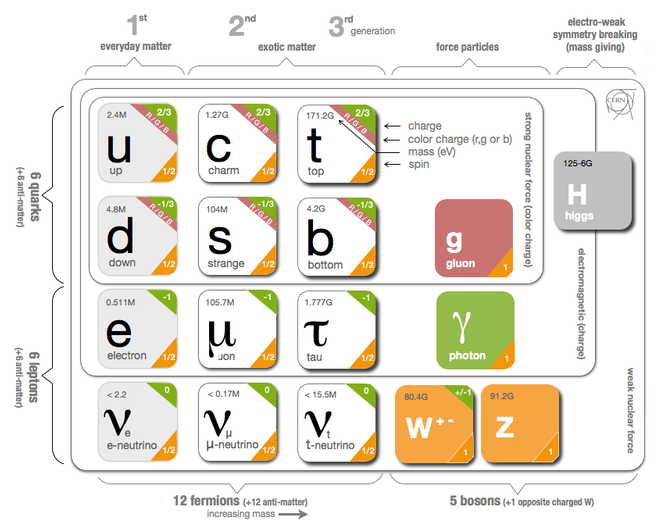
\includegraphics[width=0.95\textwidth]{Figures/HiggsPairProduction/sm.png}
\caption[Standard Model of elementary particles and interactions]{Standard model of elementary particles and interactions~\cite{Purcell:1473657}.}
\label{fig:sm}
\end{figure}

\subsection{The Fermion and Gauge Sectors}
In QFT, the requirement of gauge invariance or symmetry of the Lagrangian density under local phase transformations of a mathematical group introduces the presence of massless boson fields, which are interpreted as the quanta mediating the interaction. One example of a gauge QFT is quantum electrodynamics (QED). The predictions of QED have been successfully tested by very high-precision experiments~\cite{Karshenboim:2005iy}. The Lagrangian density of the electron field ($\Psi$) interacting with an electromagnetic field is defined as $\mathrm{\mathcal{L}_{QED}=-\frac{1}{4}F_{\mu\nu}F^{\mu\nu} + i\overline{\Psi} D_{\mu} \gamma^{\mu} \Psi - m_{e}\overline{\Psi}\Psi }$, where $\mathrm{F_{\mu\nu}=\partial_{\mu}A_{\nu}-\partial_{\nu}A_{\mu} }$ is the electromagnetic field strength, $\mathrm{A_{\mu}}$ is the photon field introduced by gauge invariance, $\mathrm{ D_{\mu}=\partial_{\mu}-iqA_{\mu} }$ is the covariant derivative, and q is the absolute value of electron electric charge. The $\mathrm{\mathcal{L}_{QED}}$ Lagrangian density is invariant under the $\mathrm{U(1)_{Q}}$ group local transformations of the electron and photon fields: $\mathrm{\Psi^{'}(x)=e^{iq\alpha(x)}\Psi(x)}$ and $\mathrm{A^{'}_{\mu} = A_{\mu} - \frac{1}{q}\partial_{\mu}\alpha(x)}$, respectively. Note that $\mathrm{\mathcal{L}_{QED}}$ is not invariant if there is mass term associated to the photon field is imposed (e.g. $\frac{1}{2}m_{A}^{2}~A^{\mu}A_{\mu}$)~\cite{peskin,costa,pdg}.

The SM is a generalization of the fundamental interactions under the $\mathrm{SU(3)_{C} \bigotimes SU(2)_{L}\bigotimes U(1)_{Y} }$ group. The strong interaction is studied by quantum chromodynamics (QCD) based on the $\mathrm{SU(3)_{C}}$ color group. In QCD, colored fermion fields (quarks) represented by SU(3) color triplets $\mathrm{q=\icol{q_{1}\\q_{2}\\q_{3}}}$ interact via 8 massless gauge boson fields (gluons) corresponding to the $\mathrm{SU(3)_{C}}$ generators. Both quarks and gluons have three possible color charges: red (r), blue (b) and green (g). The strength of the interaction is quantified by the strong coupling constant $\mathrm{g_{s}}$ (or $\mathrm{\alpha_{s} = \frac{g_{s}}{4\pi}}$). An important result of the QCD formulation is a phenomenon known as asymptotic freedom. At low-energy scales ($Q^{2}$), the value of the $\alpha_{s}$ strength increases, dictating the confinement of quarks and gluons within color-neutral composite particles named as hadrons (e.g. the proton). At high energies scales, the $\alpha_{s}$ strength decreases ($\mathrm{\alpha_{s}<<1}$), allowing the experimental study of the hadron constituents often named partons. The inner structure of hadrons are made of valence quarks, gluons and quark-antiquark pairs, which are described by the Parton Distribution Function (PDF). There are no free quarks observed in nature because they almost instantaneously ($10^{-24}-10^{-23}$s) become part of hadrons within a collimated shower of particles (hadronic jets) through a process named hadronization (except the top quark which decays at $\sim10^{-25}$ s)~\cite{costa,pdg}. 

The electromagnetic and weak interactions are studied in a unified manner by the electroweak (EW) theory based on the $\mathrm{SU(2)_{L}\bigotimes U(1)_{Y} }$ group~\cite{Weinberg:1967tq,Salam:1968rm,Glashow:1961tr}. Experimental measurements show that only fermions with left-handed chirality interact via charged weak interactions. The right-handed (R) and left-handed (L) chirality components of a fermion field $\Psi$ are obtained using projection operators as  $\mathrm{\Psi_{R/L}}=\frac{1\pm\gamma^{5}}{2} \Psi$. In the EW formalism, the massless gauge bosons are $\mathrm{W_{\mu}^{i}(i=1,2,3)}$ and $\mathrm{B_{\mu}}$. They mediate interactions for fermions with non-zero isospin I and hypercharge Y, respectively. The relation between electric charge (Q), third component of isospin ($\mathrm{I_{3}}$) and hypercharge (Y) is $\mathrm{Q=I_{3} + \frac{Y}{2} }$. The left-handed fermions ($I\neq0$) are represented by the SU(2) doublets $\mathrm{\icol{\nu_{\ell} \\ \\ \ell^{-}}_{L}}$ and $\mathrm{\icol{u \\ \\ d }_{L}}$, respectively. The right-handed fermions ($I=0$) are represented by SU(2) singlets ($\mathrm{\ell^{-}_{R}}$, $\mathrm{u_{R}}$ and $\mathrm{d_{R}}$). 

The experimental short range nature of weak interactions implies the existence of massive vector bosons. Furthermore, observed fermions like the electron are massive particles. However, explicit mass terms associated to the gauge boson and fermion fields are forbidden in the EW Lagrangian density due to $\mathrm{SU(2)_{L}\bigotimes U(1)_{Y} }$ gauge symmetry. Therefore, the formulation needs a gauge invariant mechanism to generate these masses~\cite{costa,pdg}.

\subsection{The Scalar Sector}
The Brout-Englert-Higgs (BEH) mechanism solves elegantly the mass-generation paradigm without violating gauge symmetry~\cite{Higgs:1964ia,Englert:1964et,Guralnik:1964eu}. It adds a complex scalar doublet $\Phi$ with a Lagrangian density $\mathrm{\mathcal{L}_{BEH}=\mathcal{D}_{\mu}^{\dagger}\Phi \mathcal{D}^{\mu}\Phi-V(\Phi)}$ , where $\mathrm{V(\Phi) = - \mu^{2} (\Phi^{\dagger}\Phi ) + \lambda (\Phi^{\dagger}\Phi )^{2}  }$ and $\mu^{2},\lambda>0$~\cite{costa,pdg}.

In the BEH mechanism, $\Phi$ develops a vacuum expectation state ($\mathrm{\langle\Phi\rangle_{0}}$) that satisfies the condition: \hbox{$\mathrm{\langle\Phi^{\dagger}\Phi\rangle_{0} = \frac{\mu^{2}} {2\lambda} = \frac{\nu^{2}}{2}}$}, where $\nu$ is known as the vacuum expectation value (vev). This leads to a `spontaneous' breaking of the electroweak symmetry group $\mathrm{SU(2)_{L}\bigotimes U(1)_{Y}}$ (or EWSB) to the electromagnetic group $\mathrm{U(1)_{Q}}$ with a massless photon, and generating the masses to the charged- and neutral-current weak bosons W$^{\pm}$ and Z, respectively. Furthermore, a real scalar field named the Higgs field H is introduced with its massive particle, popularly known as the Higgs boson. Table~\ref{Tab:higgs} summarizes the BEH Lagrangian terms after EWSB. Finally, charged fermion fields acquire masses through Higgs-fermion Yukawa interactions seen Figure~\ref{fig:hinteractions}~E), where fermion masses are given by $\mathrm{m_{f}=\frac{y_{f}\nu}{\sqrt{2}}}$, and $\mathrm{y_{f}}$ is the associated Yukawa coupling. Neutrino fields remain massless in the theory~\cite{costa,pdg}.

One important prediction is the structure of the Higgs boson potential (See Table~\ref{Tab:higgs}) with the associated cubic and quartic Higgs self-interactions via the self-couplings $\mathrm{\lambda_{HHH}}$ and $\mathrm{\lambda_{HHHH}}$, respectively. These self-interactions are responsible for the Higgs boson mass $\mathrm{m_{H}}$. The Higgs self-couplings are connected to the Higgs boson mass and the vev by the relation $\mathrm{\lambda_{HHH} =\lambda_{HHHH} = \frac{m_{H}^{2}} { 2 {\nu}^{2}}}$. The experimental confirmation of this relation is crucial to our understanding of the BEH mechanism and a test of the internal consistency of the SM formulation. The Higgs boson interactions predicted by the SM are illustrated in Figure~\ref{fig:hinteractions}~\cite{costa,pdg}.

\begin{table}[!htb]
\centering
\caption[BEH Lagrangian terms after the spontaneous eletroweak symmetry breaking (EWSB)]{BEH Lagrangian terms after the spontaneous eletroweak symmetry breaking (EWSB). The following variables are used  where V = W, Z: Higgs boson mass ($\mathrm{m_{H}}$), W$^{\pm}$ boson mass ($\mathrm{m_{W}}$), Z boson mass ($\mathrm{m_{Z}}$), coupling $\mathrm{g_{HVV}=\frac{2m_{V}^{2}}{\nu} }$, coupling $\mathrm{g_{VVHH}=\frac{m_{V}^{2}}{\nu^{2}}}$, and coupling $\mathrm{\lambda=\lambda_{HHH} = \lambda_{HHHH} = \frac{m_{H}^{2}} { 2 {\nu}^{2}}}$.}\label{Tab:higgs}
\begin{tabularx}{\textwidth}{XXXX}
\hline
$\mathrm{\mathcal{L}_{BEH}}$ terms after EWSB & Meaning \\
\hline
$\mathrm{\frac{1}{2}(\partial_{\mu}H)(\partial^{\mu}H)}$ & Higgs kinematic term \\[1pt]
$\mathrm{-\frac{1}{2}m_{H}^{2}H^{2} -\nu\lambda_{HHH} H^{3} -\frac{1}{4}\lambda_{HHHH} H^{4} + \frac{1}{4}\lambda \nu^{4}}  $ & Higgs potential term and self-interactions  \\[1pt]
$\mathrm{+ m_{W}^{2} H W_{\mu}^{-} W^{+,\mu} + g_{HWW} H W_{\mu}^{-} W^{+,\mu} }$ & $W^{\pm}$ mass term and HWW interaction \\[1pt]
$\mathrm{+\frac{1}{2}m_{Z}^{2}Z_{\mu}Z^{\mu} + \frac{1}{2} g_{HZZ}H Z_{\mu}Z^{\mu}}$  & Z mass term and HZZ interaction\\[1pt]
$\mathrm{+g_{WWHH} H^{2} W_{\mu}^{-} W^{+,\mu} }$ & WWHH quartic interaction\\[1pt]
$\mathrm{+\frac{1}{2} g_{ZZHH}H^{2} Z_{\mu}Z^{\mu} }$ & ZZHH quartic interaction\\[1pt]
\hline
\end{tabularx}
\end{table}

\begin{figure}[htp!]
\captionsetup[subfigure]{justification=centering}
\centering
\subfloat[]{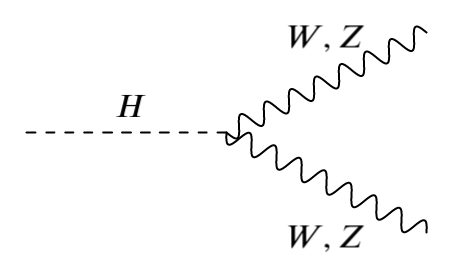
\includegraphics[width=0.30\textwidth]{Figures/HiggsPairProduction/ihvv.png}}
\subfloat[]{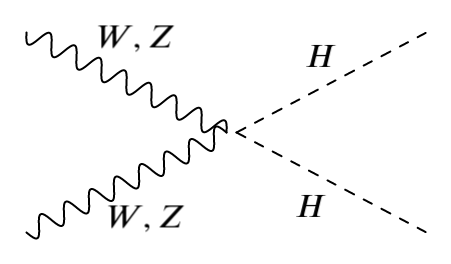
\includegraphics[width=0.30\textwidth]{Figures/HiggsPairProduction/ihhvv.png}}\\
\subfloat[]{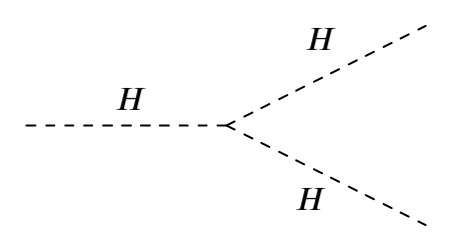
\includegraphics[width=0.30\textwidth]{Figures/HiggsPairProduction/ihhh.png}}
\subfloat[]{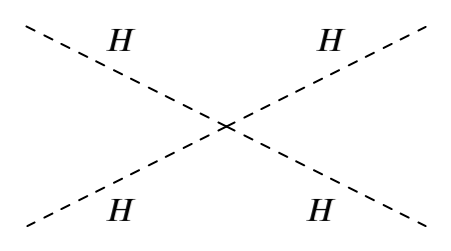
\includegraphics[width=0.30\textwidth]{Figures/HiggsPairProduction/ihhhh.png}}
\subfloat[]{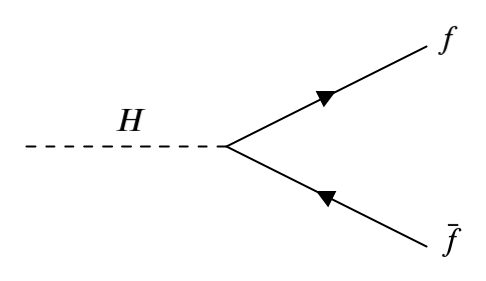
\includegraphics[width=0.30\textwidth]{Figures/HiggsPairProduction/ihf.png}}
\caption[Predicted interactions of the Higgs boson with fermions and vector bosons]{Predicted interactions of the Higgs boson (H) with fermions (f) and vector bosons (V): A) HVV interaction, B) HHVV interaction, C) HHH self-interaction, D) HHHH self-interaction, and E) Higgs-fermion Yukawa interaction.}
\label{fig:hinteractions}
\end{figure}

\subsection{The Higgs Boson}
On July $\mathrm{4^{th}}$ 2012, the CMS and ATLAS Collaborations at the LHC announced the observation of a new resonance with mass around $\hm=125$ GeV and properties compatible with the SM Higgs boson~\cite{atlashiggs,cmshiggs}.  Since then, both collaborations have performed associated precision measurements using 7, 8 and 13 TeV pp collision data, which continue to establish it as the fundamental scalar predicted by the SM. In what follows is presented a brief summary of the Higgs boson production phenomenology, decay channels, and experimental status. 

% Talk about the Higgs boson properties
\subsubsection{Production mechanisms and decay channels}
The value of $\hm$ was the only free parameter left to predict the Higgs boson phenomenology. Given that $\hm$ is known, then the production mechanisms and decays are fully determined. The Higgs boson has several production mechanisms. Gluon fusion (ggF-H) is the main production mode, and then the vector-boson fusion (VBF-H) follows it, with a production cross section of approximately one order of magnitude smaller. Then, the subdominant production modes are the following: associated production with a W or a Z boson (VH) and associated production with a top quark pair ($\mathrm{t\overline{t}H}$), among others. Examples of representative LO diagrams are shown in Figure~\ref{fig:hdiagrams}. In addition, Table~\ref{tab:higgsmodes} presents the theoretical production cross section for several modes. 

\begin{table}[htb]
\centering
\caption[Higgs boson production cross section and relative uncertainties]{\label{tab:higgsmodes} Higgs boson production cross section (in pb) and relative uncertainties (theory, PDF,$\alpha_{S}$) for several Higgs boson ($\mathrm{m_{H}=~125~GeV}$) production modes at $\sqrt{s}=$13 and 14 TeV proton-proton collisions~\cite{pdg}. The order of QCD (EW) calculation is N3LO (NLO) for ggF and NNLO (NLO) for the others.}
\begin{tabularx}{\textwidth}{XXXXXXX}
\hline
$\sqrt{s}$ [TeV] & ggF-H                          &      VBF-H                  & WH                         & ZH                         & $\mathrm{t\overline{t}H}$ & total \\
\hline
13 &  48.6$^{+4.4\%}_{-7.0\%}$ &  3.78$^{+2.2\%}_{-2.2\%}$ &  1.37$^{+2.6\%}_{-2.6\%}$  &  0.88$^{+4.1\%}_{-3.5\%}$  & 0.50$^{+6.8\%}_{-9.9\%}$ & 55.1 \\[0pt]
14 &  54.7$^{+4.4\%}_{-7.0\%}$ &  4.28$^{+2.2\%}_{-2.2\%}$ &  1.51$^{+1.9\%}_{-2.0\%}$  &  0.99$^{+4.1\%}_{-3.7\%}$  & 0.60$^{+6.9\%}_{-9.8\%}$ & 62.1 \\[0pt]
\hline
\end{tabularx}
\end{table}

\begin{figure}[ht!]
\captionsetup[subfigure]{justification=centering}
\centering
\subfloat[]{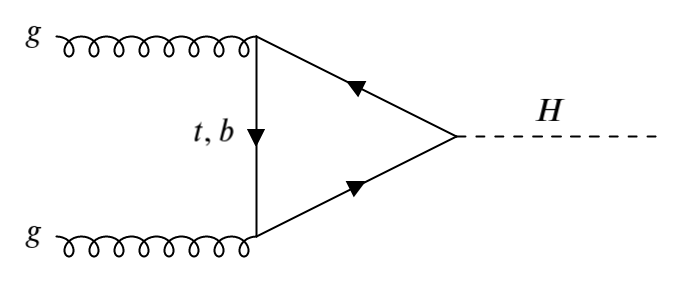
\includegraphics[width=0.33\textwidth]{Figures/HiggsPairProduction/ggfh.png}}
\subfloat[]{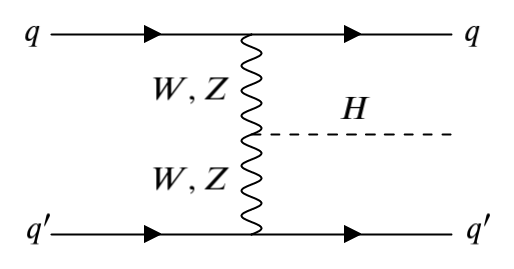
\includegraphics[width=0.25\textwidth]{Figures/HiggsPairProduction/vbfh.png}}\\
\subfloat[]{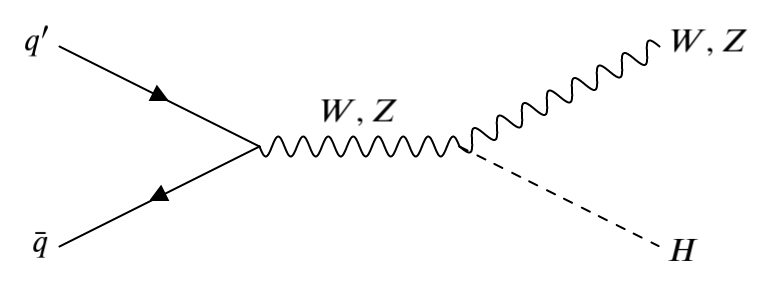
\includegraphics[width=0.33\textwidth]{Figures/HiggsPairProduction/vh.png}}
\subfloat[]{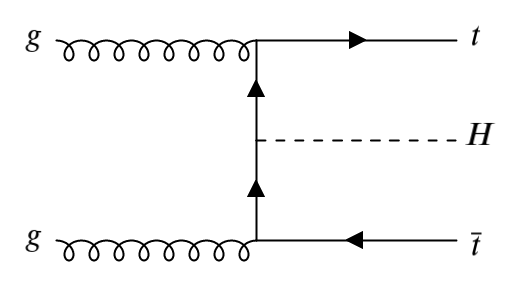
\includegraphics[width=0.25\textwidth]{Figures/HiggsPairProduction/tth.png}}\\
\caption[Examples of leading order diagrams contributing to the Higgs boson production]{Examples of leading order diagrams contributing to the Higgs boson production: A) Gluon fusion, B) Vector boson fusion, (C) Associate production with a W or Z boson, (D) Associate production with a top-quark pair.}
\label{fig:hdiagrams}
\end{figure}

The theoretical Higgs boson decay branching ratios to gauge bosons and to some fermions are presented in Table~\ref{tab:higgsbrs}. The Higgs boson decay to a bottom quark pair ($\mathrm{H\rightarrow~b\overline{b}}$) is the dominant decay channel, with around 58.2\% branching ratio. It is important to note that the Higgs boson can indirectly decay into massless particles via intermediate fermion loops: two photons ($\mathrm{H\rightarrow~\gamma\gamma}$), a Z boson and a photon ($\mathrm{H\rightarrow~Z\gamma}$), and two gluons ($\mathrm{H\rightarrow~gg}$).
\begin{table}[ht!]
\centering
\caption[Higgs boson branching ratios and relative uncertainties for several Higgs boson ($\mathrm{m_{H}=~125~GeV}$) decay modes]{\label{tab:higgsbrs} Higgs boson branching ratios and relative uncertainties for several Higgs boson ($\mathrm{m_{H}=~125~GeV}$) decay modes~\cite{pdg}.}
\begin{tabularx}{\textwidth}{XXXX}
\hline
Decay mode                                    & Branching ratio  & Relative uncertainty      \\
\hline
$\mathrm{H\rightarrow\gamma\gamma}$           & 2.22 x $10^{-3}$ & $\pm$2.1\%            \\[0pt]
$\mathrm{H\rightarrow ZZ}$                    & 2.62 x $10^{-2}$ & $\pm$1.5\%            \\[0pt]
$\mathrm{H\rightarrow W^{+}W^{-}}$            & 2.14 x $10^{-1}$ & $\pm$1.5\%            \\[0pt]
$\mathrm{H\rightarrow \tau^{+}\tau^{-}}$      & 6.27 x $10^{-2}$ & $\pm$1.6\%            \\[0pt]
$\mathrm{H\rightarrow b\overline{b}}$         & 5.82 x $10^{-1}$ & $^{+1.2\%}_{-1.3\%}$  \\[0pt]
$\mathrm{H\rightarrow c\overline{c}}$         & 2.89 x $10^{-2}$ & $^{+5.5\%}_{-2.0\%}$  \\[0pt]
$\mathrm{H\rightarrow Z\gamma}$               & 1.53 x $10^{-3}$ & $\pm$5.8\%            \\[0pt]
$\mathrm{H\rightarrow \mu^{+}\mu^{-}}$        & 2.18 x $10^{-4}$ & $\pm$1.7\%            \\[0pt]
\hline
\end{tabularx}
\end{table}

\subsubsection{Experimental Status}
The LHC exploration of the Higgs boson is carried out analyzing a broad range of production mechanisms and decay channels. The most sensitive decay channels for studying the Higgs boson are as follows. The $\mathrm{H\rightarrow~ZZ\rightarrow 4\ell~(\ell=e,\mu)}$ and $\mathrm{H\rightarrow~\gamma\gamma}$ channels have low expected rates but benefit from small background processes and have the best mass resolution ($\sim$1-2\%) due to well-reconstructed final state products. The $\mathrm{H\rightarrow~W^{+}W^{-}\rightarrow\ell^{+}\nu_{\ell}{\ell}^{\prime-}\overline{\nu}_{\ell\prime}}$ channel has relatively better rates, but the unmeasured energy from neutrinos has an impact on the resolution of the mass-related observables, e.g. the transverse mass resolution is $\sim20\%$. The $\mathrm{b\overline{b}}$ ($\tau^{+}\tau^{-}$) decay channel benefits from high rates and intermediate mass resolutions 10\% (15\%), but is affected by large and irreducible background contamination~\cite{pdg}. Challenging channels due to low very rates or large background levels are $\mathrm{H\rightarrow\mu^{+}\mu^{-}}$ and $\mathrm{H\rightarrow c\overline{c}}$, respectively.

In the LHC Run-1 (2009-2012), the ATLAS and CMS collaborations analyzed the pp collision datasets at $\sqrt{s}=7$ and 8~TeV to discover the Higgs boson~\cite{atlashiggs,cmshiggs}. The decay channels involving gauge bosons, $\mathrm{H\rightarrow~ZZ\rightarrow 4\ell~(\ell=e,\mu)}$ and $\mathrm{H\rightarrow\gamma\gamma}$ , contributed with the most significant excesses.  The $\mathrm{H\rightarrow~W^{+}W^{-}\rightarrow~\ell^{+}\nu_{\ell}{\ell}^{\prime-}\overline{\nu}_{\ell\prime}}$, $\mathrm{H\rightarrow\mathrm{b\overline{b}}}$ and $\mathrm{H\rightarrow\tau^{+}\tau^{-}}$ channels were also included but contributed with lower significance~\cite{atlashiggs,cmshiggs}. After that, studies of the spin-parity ($\mathrm{J^{P}}$) quantum numbers revealed the scalar and even-parity nature ($\mathrm{J^{P}=O^{+}}$) of the discovered particle as predicted by the SM~\cite{atlasrun1_hspinparity,cmsrun1_hmassparityspin}. The Run-1 Combined ATLAS and CMS Higgs boson mass measurement yields a value of $\mathrm{m_{H}=125.09\pm~0.24~GeV}$ using $\mathrm{H\rightarrow~ZZ\rightarrow 4\ell~(\ell=e,\mu)}$ and $\mathrm{H\rightarrow\gamma\gamma}$, benefiting from their excellent mass resolution~\cite{atlascmsrun1hmass}.

In the LHC Run-2 (2015-2018), ATLAS and CMS experiments had an excellent operation performance collecting high-quality data at $\sqrt{s}=13$~TeV, corresponding to approximately 6 times the LHC Run-1 dataset integrated luminosity. Measurements of the mass, couplings, differential and fiducial cross sections have been performed with the partial and full dataset by ATLAS~\cite{atlasrun2mes,atlasrun2hmass} and CMS~\cite{cmsrun2mes,cmsbesthmassrun2}. The Higgs boson mass measurement has been performed using the $\mathrm{H\rightarrow~ZZ\rightarrow 4\ell~(\ell=e,\mu)}$ and $\mathrm{H\rightarrow\gamma\gamma}$ decay channels. The distribution of the di-photon invariant mass in the 2016 data is presented in Figure~\ref{fig:LHCHiggsmeasurements}~A). The best mass measurement yields a value of $\mathrm{m_{H}=125.38\pm0.14~GeV}$ from the CMS combination of Run-1 and 2016 datasets~\cite{cmsbesthmassrun2}. 

Both experiments have presented the observation of the Higgs coupling to third generation fermions studying the $\mathrm{H\rightarrow~b\overline{b}}$~\cite{atlasrun2_hbb,cmsrun2_hbb} and $\mathrm{H\rightarrow\tau^{+}\tau^{-}}$~\cite{atlasrun2_htautau,cmsrun2_htautau} decays, and the $\mathrm{ttH}$ production mode~\cite{atlasrun2_tth,cmsrun2_tth}. In particular, the measurement of $\mathrm{H\rightarrow~b\overline{b}}$ decays was believed to be impossible to achieve due to the large multi-jet background and intermediate mass resolution. However, novel analysis methods based on machine learning (ML) were developed for object identification, reconstruction and signal identification, to maximize the search sensitivity. Figure~\ref{fig:LHCHiggsmeasurements} B) illustrates the distribution signal-to-background ratio bins in the $\mathrm{H\rightarrow~b\overline{b}}$ measurement. The CMS experiment found the first evidence for the Higgs coupling to the second generation fermions in the analysis of the $\mathrm{H\rightarrow\mu^{+}\mu^{-}}$ decay channel~\cite{cmsrun2_hmumu}. ATLAS show the first evidence for the $\mathrm{H\rightarrow~(\gamma/Z)^{*}\gamma~\rightarrow\ell\ell\gamma}$ decay channel~\cite{atlasrun2_h_zgamma}. Lastly, both experiments are currently developing methods to measure the $\mathrm{H\rightarrow c\overline{c}}$ decay but the development of more sophisticated methods and more data are needed to measure it in the future~\cite{atlasrun2_hcc,cmsrun2_hcc}. The Figure~\ref{fig:LHCHiggsmeasurements} C) shows the Higgs coupling measurements using CMS Run-2 data.
%Most of the signal significance comes from the analysis of the VH production mode with vector bosons decaying into 0, 1, 2 charged leptons ($\mu$ or e).
\begin{figure}[ht!]
\captionsetup[subfigure]{justification=centering}
\centering
\subfloat[]{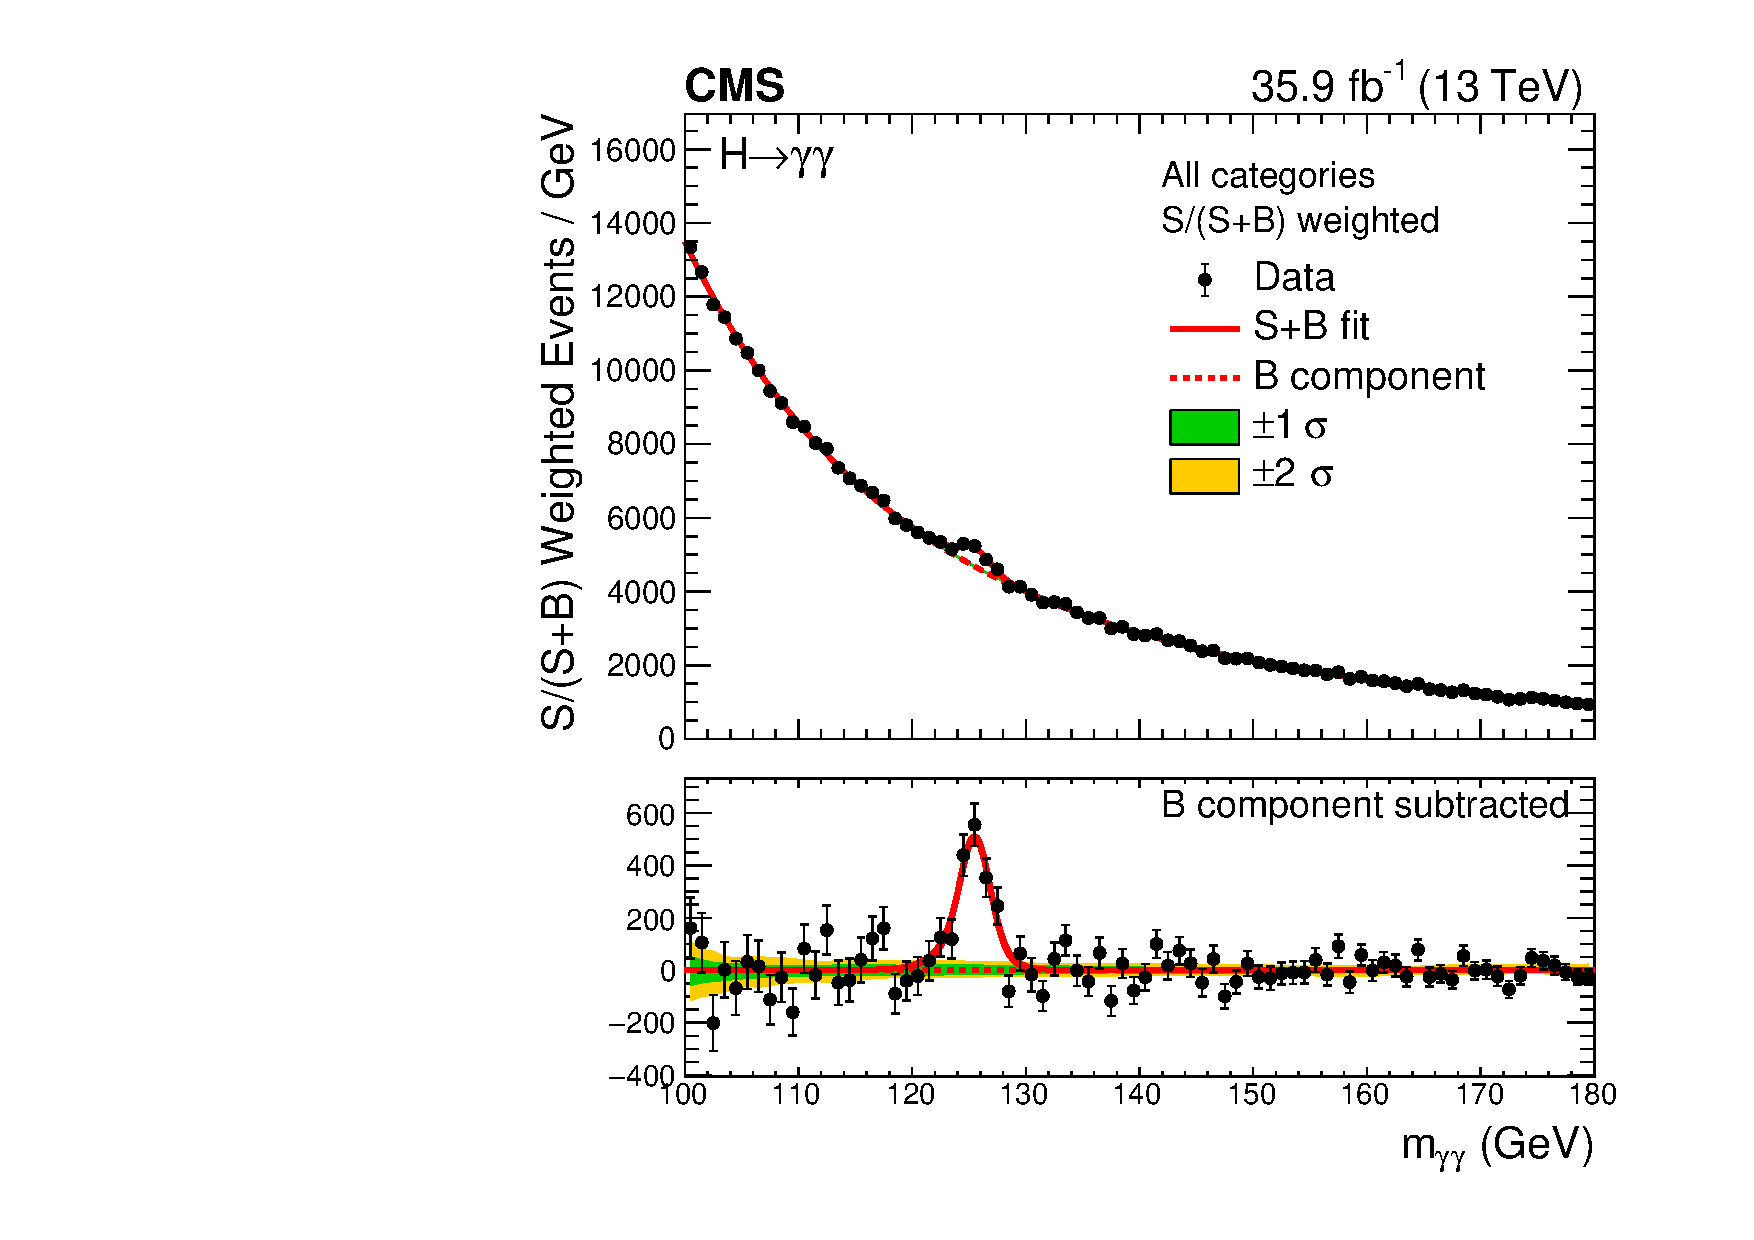
\includegraphics[width=0.32\textwidth]{Figures/HiggsPairProduction/2016higgsggmass.pdf}}
\subfloat[]{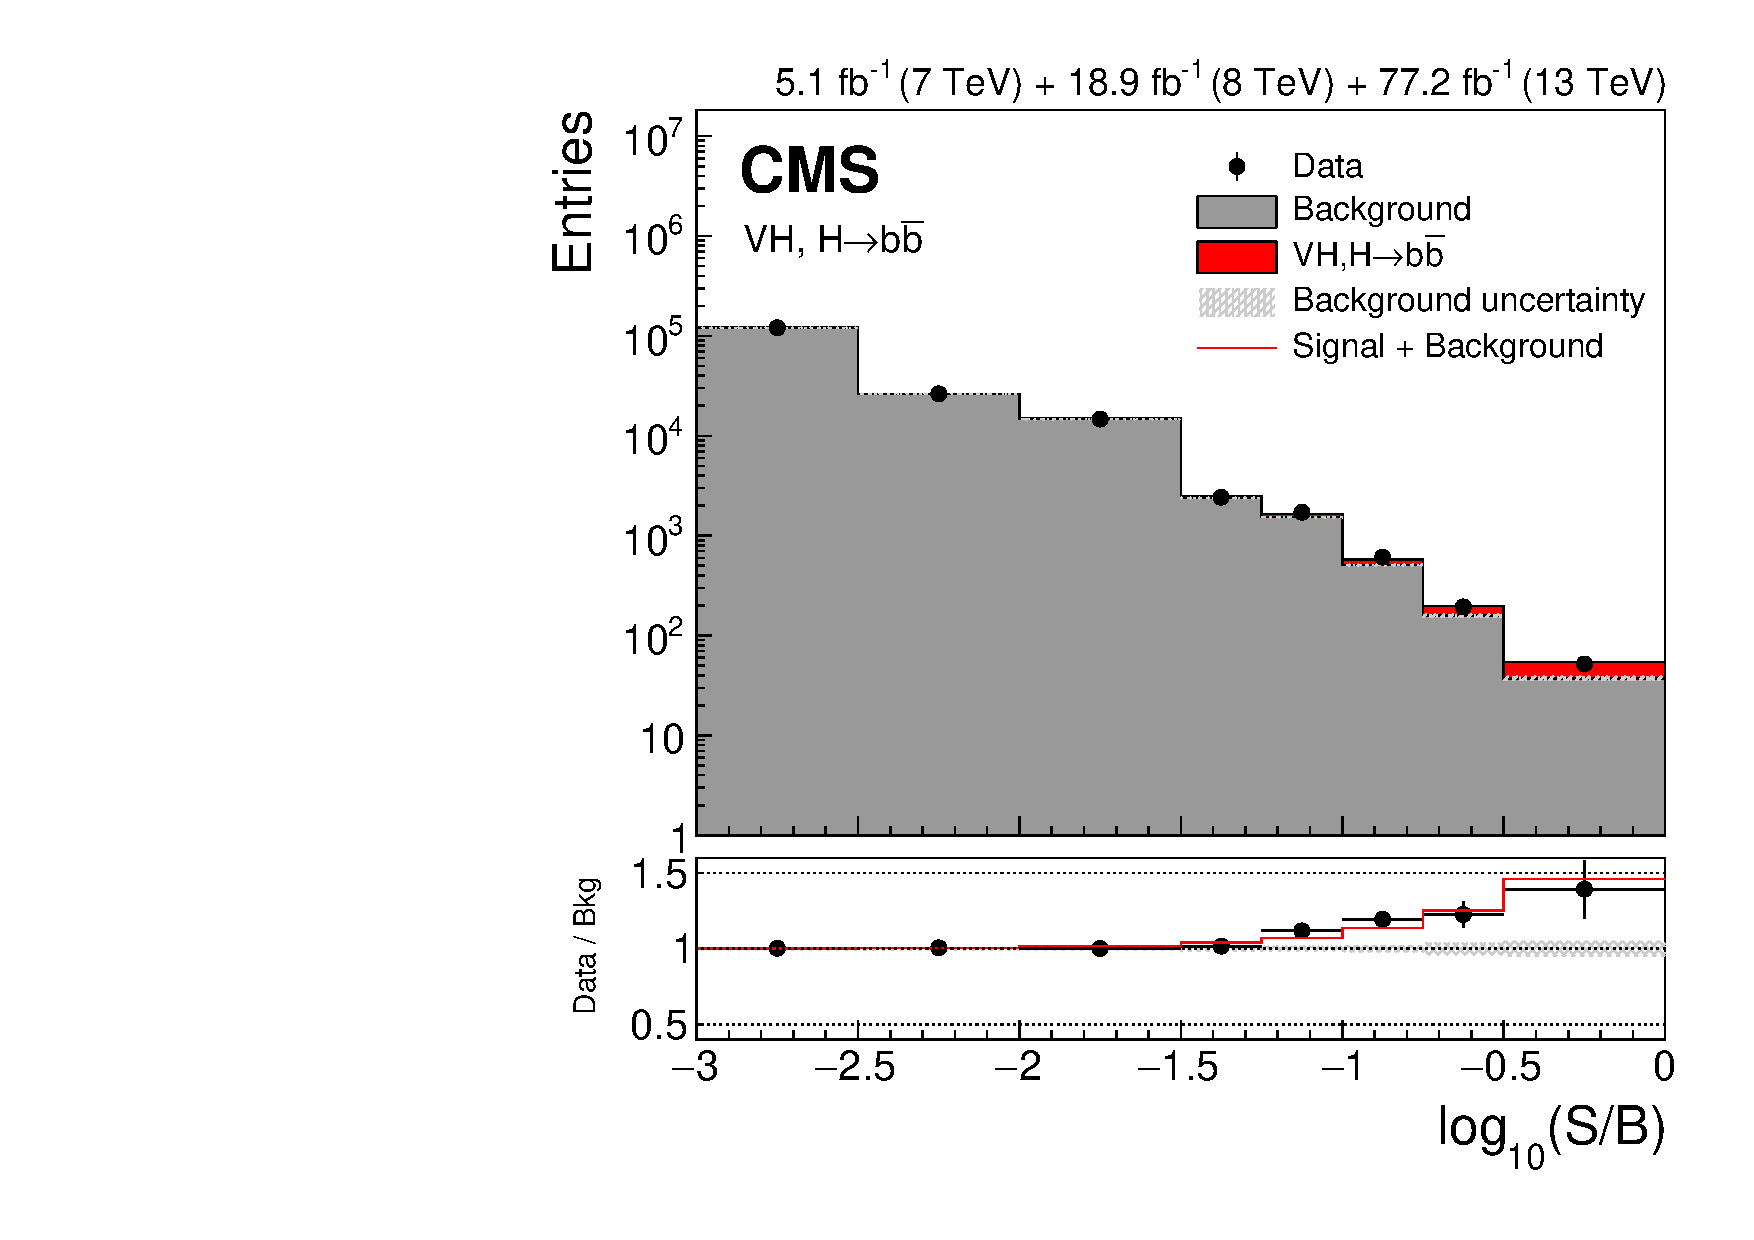
\includegraphics[width=0.32\textwidth]{Figures/HiggsPairProduction/higgsbbsb.pdf}}\\
\subfloat[]{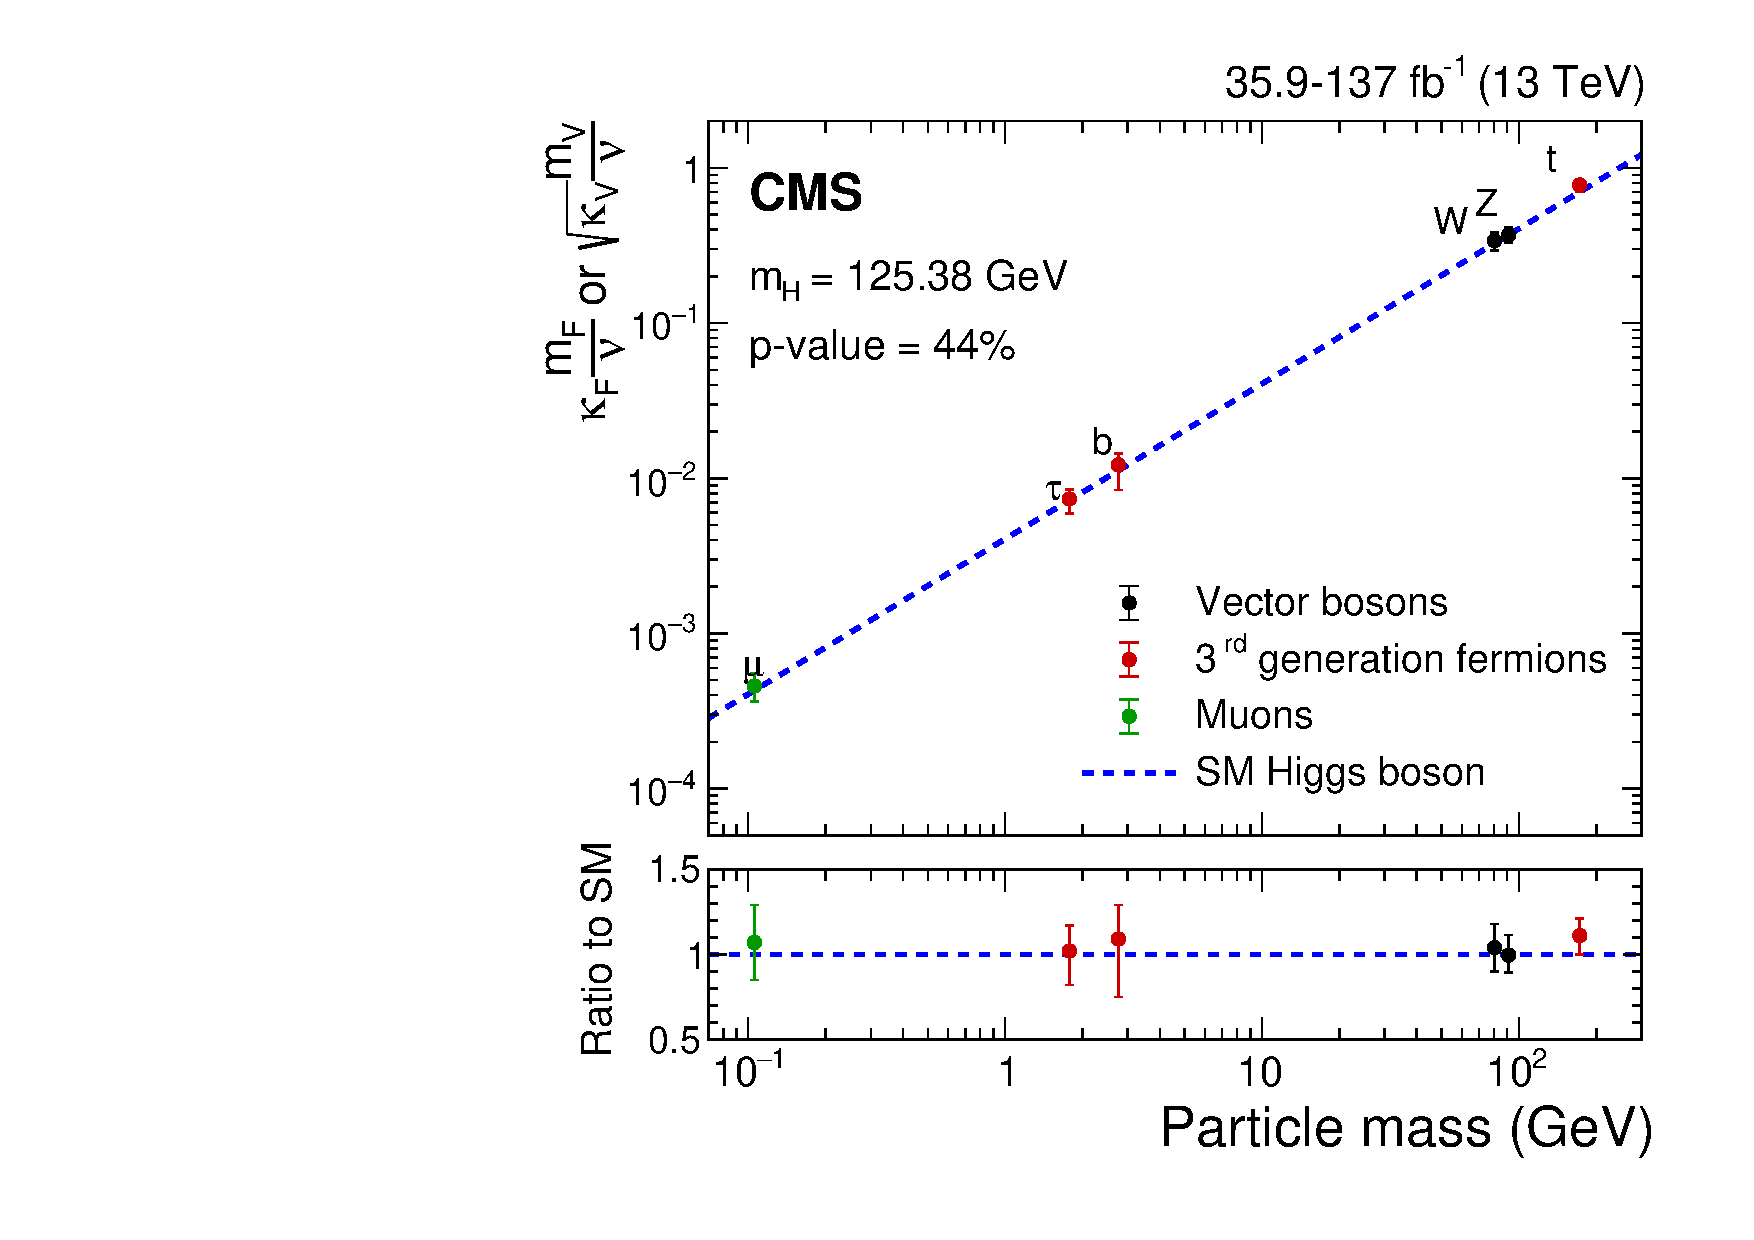
\includegraphics[width=0.32\textwidth]{Figures/HiggsPairProduction/higgscouplingsrun2.pdf}}
\caption[Selected CMS Higgs physics results in Run-2]{Selected CMS Higgs physics results in Run-2. A) Di-photon mass distribution from the 2016 dataset mass measurement~\cite{cmsbesthmassrun2}, B) Distribution of event yields sorted into bins of similar signal-to-background ratio in the observation of Higgs coupling to two bottom-quarks~\cite{cmsrun2_hbb}, C) Measurement of the Higgs couplings~\cite{cmsrun2_hmumu}.}
\label{fig:LHCHiggsmeasurements}
\end{figure}
   
\clearpage
\section{Higgs Boson Pair Production}
This section is a review of the theoretical aspects and phenomenology associated to the Higgs boson pair (HH) production. First, the physics of SM HH production is discussed. Then, the motivation and characteristics of the BSM HH production are summarized. 

\subsection{Standard Model Production}
From the precise measurement of the Higgs boson mass, the value of the Higgs self-couplings are fully predicted. The Higgs trilinear coupling or self-coupling $\mathrm{\lambda_{HHH} = \frac{m_{H}^{2}} { 2 {\nu}^{2}}\sim0.13}$, where, $\nu$ is around 246 GeV from measurements of the Fermi constant $G_{F}$. Non-resonant HH production is the only SM process with direct access to measure $\mathrm{\lambda_{HHH}}$ at the LHC. The main production mechanisms are the following, ordered by their cross section (see Table~\ref{tab:hhxs}): Gluon fusion production (ggF), vector boson fusion production (VBF), associated production with a Z or W boson (VHH) and top quark pairs associated production ($\mathrm{t\overline{t}HH}$). Some representative LO Feynman diagrams for each mode are illustrated in Figure~\ref{fig:hhdiagrams}. Note that single Higgs production has indirect access to the $\mathrm{\lambda_{HHH}}$ coupling via NLO EW corrections~\cite{Degrassi:2016wml,Maltoni:2017ims}.

\begin{table}[htb]
\centering
\caption[Higgs boson pair production cross section (in pb) and relative uncertainties]{\label{tab:hhxs} Higgs boson pair production cross section (in fb) and relative uncertainties for several Higgs boson ($\mathrm{m_{H}=~125~GeV}$) production modes at $\sqrt{s}=$13 and 14 TeV proton-proton collisions~\cite{DiMicco:2019ngk}.}
\begin{tabularx}{\textwidth}{XXX}
\hline
$\sqrt{s}$                  & 13 TeV                               & 14 TeV                                 \\
\hline
$\mathrm{ggF}$              & 31.05$^{+6.0\%}_{-23.0\%}\pm3.0\%$   &  36.69$^{+6.0\%}_{-23.0\%}\pm3.0\%$     \\[0pt]
$\mathrm{VBF}$              &   1.73$^{+0.03\%}_{-0.04\%}\pm2.1\%$ &  2.05$^{+0.03\%}_{-0.04\%}\pm2.1\%$    \\[0pt]
$\mathrm{ZHH}$              &  0.363$^{+3.4\%}_{-2.7\%}\pm1.9\%$   &  0.415$^{+3.5\%}_{-2.7\%}\pm1.8\%$     \\[0pt]
$\mathrm{W^{+}HH}$          &  0.329$^{+0.32\%}_{-0.41\%}\pm2.2\%$ &  0.369$^{+0.33\%}_{-0.39\%}\pm2.1\%$   \\[0pt]
$\mathrm{W^{-}HH}$          &  0.173$^{+1.2\%}_{-1.3\%}\pm2.8\%$   &  0.198$^{+1.2\%}_{-1.3\%}\pm2.7\%$     \\[0pt]
$\mathrm{t\overline{t}HH}$  &  0.773$^{+1.5\%}_{-4.3\%}\pm3.2\%$   &  0.949$^{+1.7\%}_{-4.5\%}\pm3.1\%$     \\[0pt]
\hline
\end{tabularx}
\end{table}

In the dominant mode, gluon fusion, Higgs boson pairs proceed from quantum loops involving mainly top-quarks (and a small b-quark contribution). At LO, a triangle-loop diagram and a box-loop diagram contribute to the ggF mode physics (see Figure~\ref{fig:hhdiagrams}~A)). The triangle-loop diagram contains the Higgs self-coupling $\mathrm{\lambda_{HHH}}$, while the box diagram contains the top quark Yukawa coupling ($\mathrm{y_{t}}$). There is a large negative interference between the two loop diagrams, resulting in a very small production cross section. The individual contributions to the cross section from the box, triangle and their interference are illustrated as function HH invariant mass in Figure~\ref{fig:hhmcont}. The triangle or self-interaction diagram contribution is mostly located at low HH mass values (i.e. soft spectrum) and is largely suppressed by the interference contribution.

\begin{figure}[htp!]
\centering
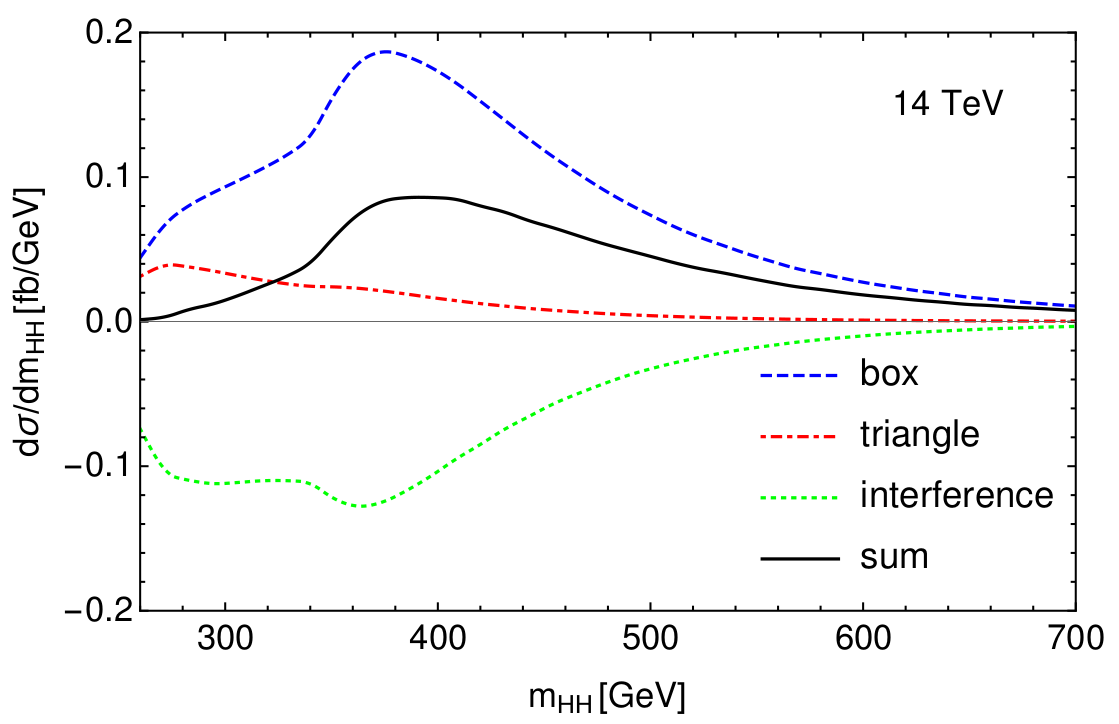
\includegraphics[width=1.0\textwidth]{Figures/HiggsPairProduction/mhhcont.png}
\caption[Differential cross section distribution as a function of the Higgs boson invariant mass]{Differential cross section distribution as a function of the Higgs boson invariant mass at leading order~\cite{DiMicco:2019ngk}. The contributions to the gluon fusion production cross section (black line) are presented: box (dashed blue), triangle (dashed red), interference (dashed green).}
\label{fig:hhmcont}
\end{figure}

The secondary production mode, vector boson fusion (VBF), has three LO contributing diagrams shown in Figure~\ref{fig:hhdiagrams}~B). The VBF production cross section is approximately one order of magnitude smaller than the ggF one but has a very characteristic signature with two quark hadronic jets with large invariant mass and separation in the final state. Besides having an extra handle on the $\mathrm{\lambda_{HHH}}$ coupling, this process has a unique access to study the interaction between two vector bosons and two Higgs bosons through the $\mathrm{g_{HHVV}}$ coupling. Moreover, this mode has access to the interaction between the Higgs boson and two vector bosons via the $\mathrm{g_{HVV}}$ coupling. 

\begin{figure}[ht]
\captionsetup[subfigure]{justification=centering}
    \centering
      \begin{subfigure}{\textwidth}
  \centering
          \caption{}
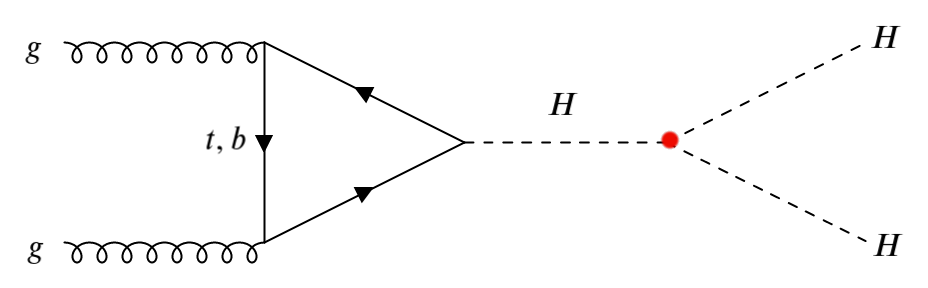
\includegraphics[width=0.40\textwidth]{Figures/HiggsPairProduction/ggf1.png}
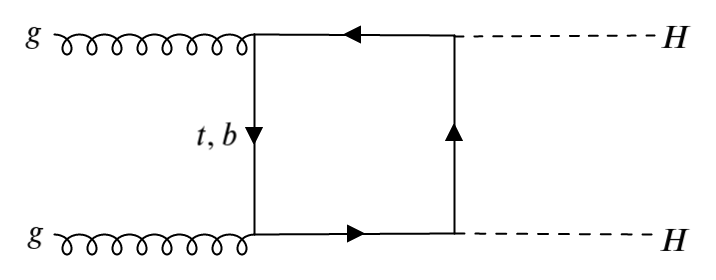
\includegraphics[width=0.30\textwidth]{Figures/HiggsPairProduction/ggf2.png}\\
      \end{subfigure}
      \begin{subfigure}{\textwidth}
  \centering
          \caption{}
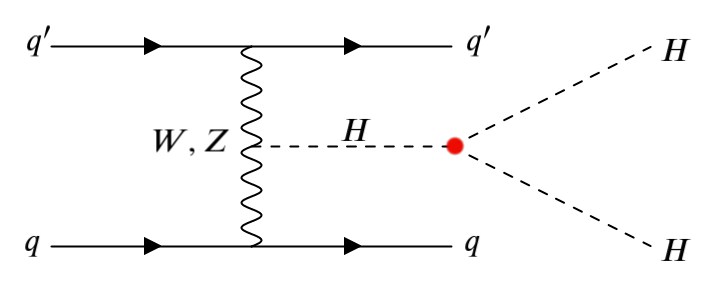
\includegraphics[width=0.32\textwidth]{Figures/HiggsPairProduction/vbf2.png}
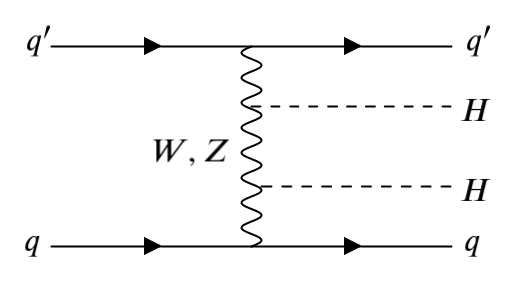
\includegraphics[width=0.23\textwidth]{Figures/HiggsPairProduction/vbf1.png}
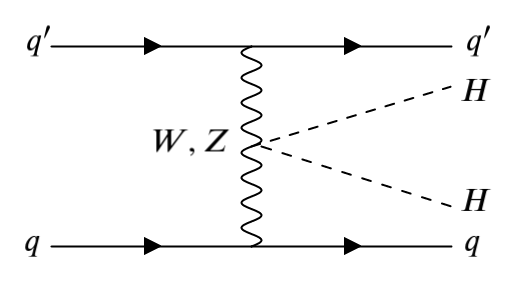
\includegraphics[width=0.23\textwidth]{Figures/HiggsPairProduction/vbf3.png}\\
      \end{subfigure}
      \begin{subfigure}{\textwidth}
  \centering
          \caption{}
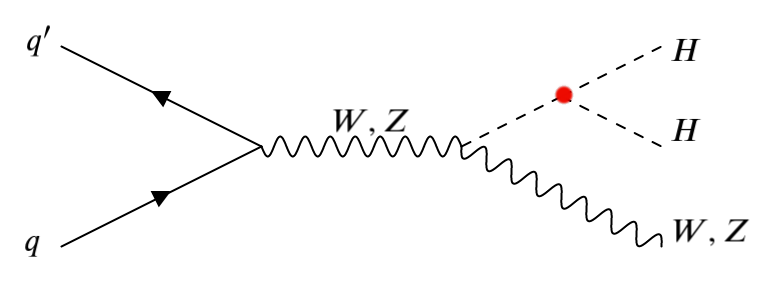
\includegraphics[width=0.32\textwidth]{Figures/HiggsPairProduction/vhh1.png}
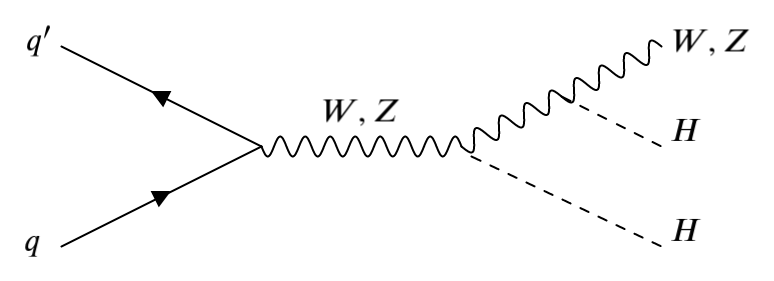
\includegraphics[width=0.32\textwidth]{Figures/HiggsPairProduction/vhh2.png}
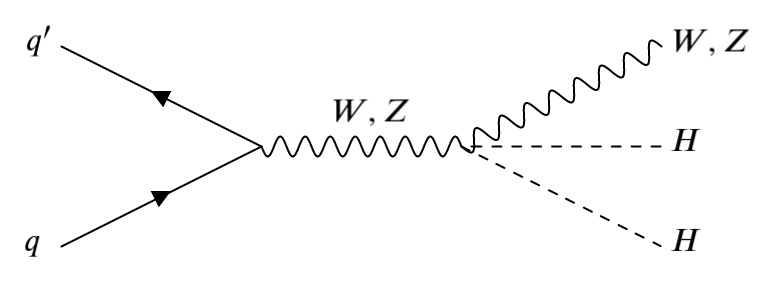
\includegraphics[width=0.32\textwidth]{Figures/HiggsPairProduction/vhh3.png}\\
      \end{subfigure}
      \begin{subfigure}{\textwidth}
  \centering
          \caption{}
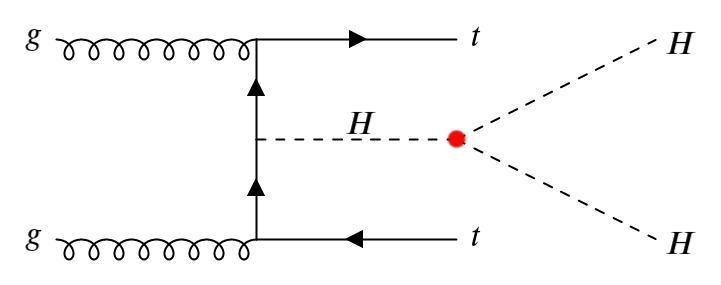
\includegraphics[width=0.30\textwidth]{Figures/HiggsPairProduction/tthh1.png}
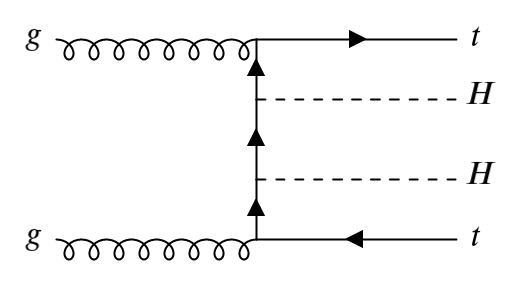
\includegraphics[width=0.22\textwidth]{Figures/HiggsPairProduction/tthh2.png}\\
      \end{subfigure}
\caption[Examples of leading order (LO) diagrams contributing to the Higgs boson pair production mode mechanisms]{Examples of leading order (LO) diagrams contributing to the Higgs boson pair production mode mechanisms. A) Gluon fusion, B) Vector boson fusion C) Associate production with a W or Z boson, D) Associate production with top-quark pair. The red circle represents the Higgs self-coupling $\mathrm{\lambda_{HHH}}$.}
\label{fig:hhdiagrams}
\end{figure}

\subsection{Beyond the Standard Model Production} \label{hh:BSMcouplings}
Although the SM have been successfully in predicting the measurements at particle colliders, it does not provide explanations to many experimental and theoretical aspects about nature. Many of them are connected to the scalar sector, which hints that BSM physics is hidden there. From the theoretical point of view, there is no fundamental symmetry to protect the Higgs boson mass from quadratically divergent radiative corrections~\cite{pdg}. Furthermore, a metastable scalar potential appears to be favored based on the measured Higgs boson and top-quark masses, challenging the long-term stability of the Universe~\cite{Elias-Miro:2011sqh}.

Many BSM physics scenarios are able to regulate the shortcomings of the SM. Some of these models have extra singlets~\cite{Robens,Dawson:2015haa}, extra doublets inspired by the next-to-minimal supersymmetric extension of the SM(NMSSM)~\cite{Ellwanger:2009dp,Djouadi}, or warped extra-dimensions with a new scalar or a graviton~\cite{RandallSundrum,Oliveira:2014kla}.  A broad class of these models predict the production of new particles (X) that can subsequently decay in a sizeable branching fraction to a pair of Higgs boson ($\mathrm{X\rightarrow~HH}$)~as illustrated in the diagrams in Figure~\ref{fig:resonances}. At the LHC, one can probe these BSM models using a common experimental signature consisting of an enhancement of the cross section at the X mass ($\mathrm{m_{X}}$). The studied masses range from 250 GeV ($\mathrm{m_{X}>2~m_{H}}$) to a few TeVs. Recent theoretical work has also highlighted the possibility of spectacular multi-scalar resonant decays into a new scalar (Y) and a Higgs boson ($\mathrm{X\rightarrow YH}$), and a Higgs boson triplet ($\mathrm{X\rightarrow YH\rightarrow HHH}$) ~\cite{Ellwanger:2017skc,Robens:2019kga}.

\begin{figure}[htp!]
\centering
\captionsetup[subfigure]{justification=centering}
\subfloat[]{\centering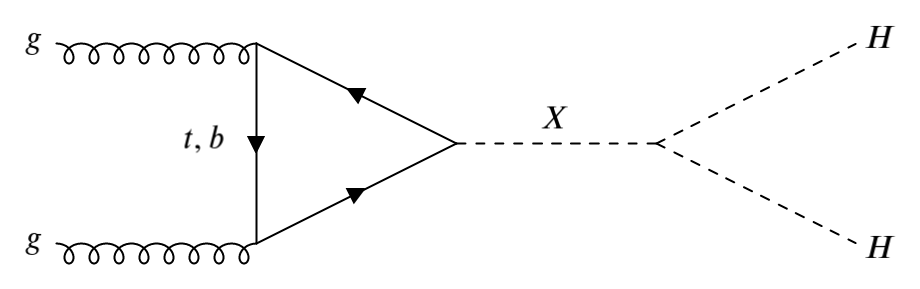
\includegraphics[width=0.50\textwidth]{Figures/HiggsPairProduction/xggf.png}}
\subfloat[]{\centering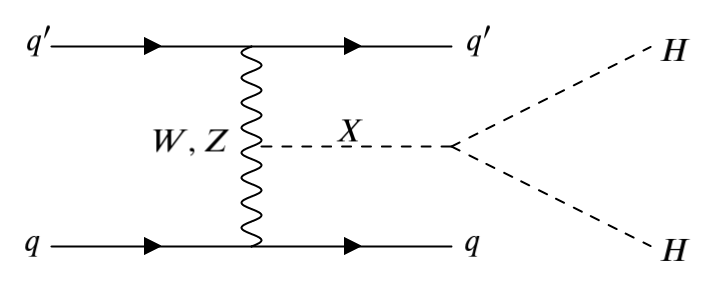
\includegraphics[width=0.43\textwidth]{Figures/HiggsPairProduction/xvbf.png}}\\
\caption[Diagrams of production of a new resonances decaying to a Higgs boson pair at the LHC]{Diagrams of production of a new resonances decaying to a Higgs boson pair at the LHC: A) Gluon fusion production mode, and B) Vector boson production mode.}
\label{fig:resonances}
\end{figure}

If the scale of the new physics is beyond the direct reach of the LHC, the effects of the new particles and their interactions within quantum loops may result in modifications of the HH production cross section and kinematics. These modifications can be parametrized with respect to the SM value through coupling modifiers($\kappa$). For instance, anomalous Higgs self-coupling, $\mathrm{g_{HVV}}$ coupling and  $\mathrm{g_{VVHH}}$ coupling have the modifiers $\mathrm{\kappa_{\lambda}=\lambda_{HHH}/\lambda^{SM}_{HHH}}$, $\mathrm{\kappa_{V}}$, and $\mathrm{\kappa_{2V}}$ , respectively. Figure~\ref{fig:klambdaxs} presents the dependence of the cross section for different production modes as a function of the $\mathrm{\kappa_{\lambda}}$ modifier (assuming other couplings are set to their SM values). The ggF mode cross section has a quadratic $\mathrm{\kappa_{\lambda}}$-dependence, with a minimum at around 2.45 (maximal interference effect). 

\begin{figure}[ht]
\centering
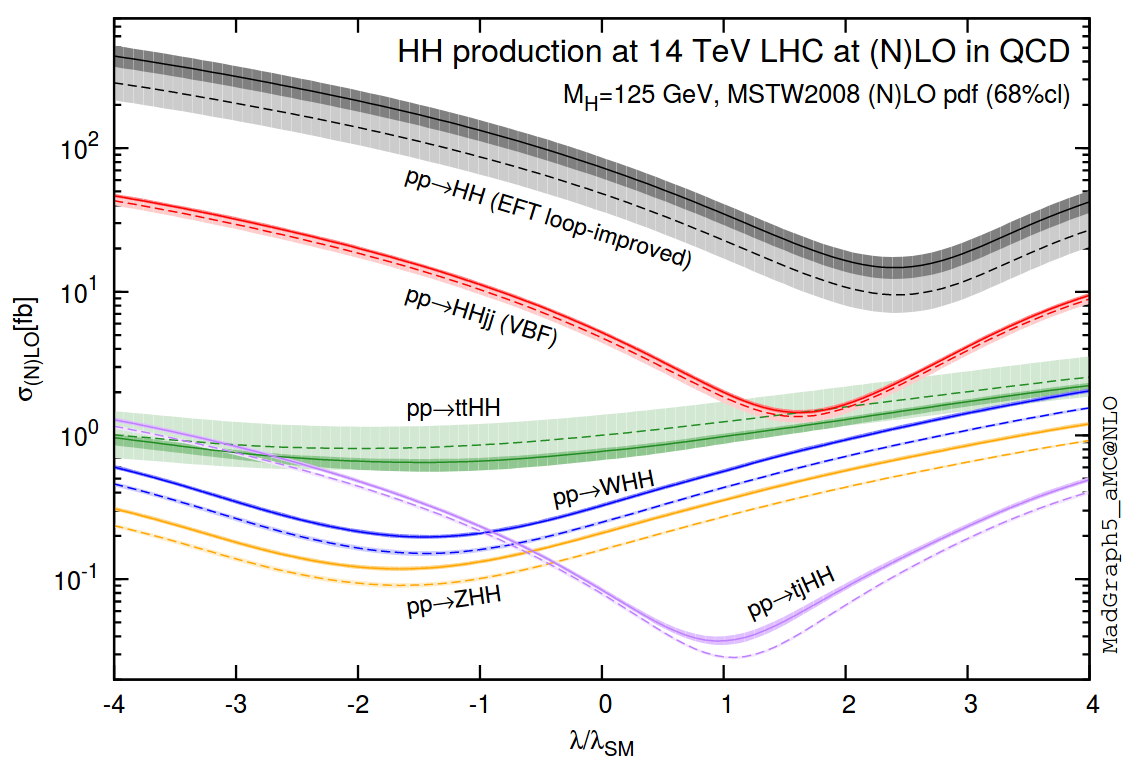
\includegraphics[width=0.9\textwidth]{Figures/HiggsPairProduction/klambdaxs.png}
\caption[Higgs boson pair production cross section at $\sqrt{s}=14$ TeV LHC proton-proton collisions for various modes]{Higgs boson pair production cross section at $\sqrt{s}=14$ TeV LHC proton-proton collisions for various modes calculated at the LO and NLO precision in QCD, as a function of the Higgs self-coupling with respect to the SM ($\mathrm{\lambda/\lambda_{SM}}$)~\cite{Frederix:2014hta}. The dashed (solid) lines and light- (dark-)color bands correspond to the LO (NLO) results and to the scale and PDF uncertainties added linearly.}
\label{fig:klambdaxs}
\end{figure}

BSM $\mathrm{\kappa_{\lambda}}$ values ($\mathrm{\kappa_{\lambda}\neq1}$)  modify the kinematic properties of the Higgs boson pair. This effect is illustrated on Figure~\ref{fig:mhhvariation} A), where the HH invariant mass spectrum for different values of the $\mathrm{\kappa_{\lambda}}$ modifier in the ggf mode is shown. The softest spectrum (experimentally challenging due to event selection thresholds), corresponds to $\mathrm{\kappa_{\lambda}=5}$. Note that the case where mostly the triangle diagram contributes to the HH production cross section ($\mathrm{\kappa_{\lambda}=20}$) has a soft spectrum, whereas the case of box diagram ($\mathrm{\kappa_{\lambda}=20}$) has an intermediate mass spectrum. For the $\mathrm{\kappa_{\lambda}=2.45}$ case, a spectrum with a low mass peak and intermediate mass peak is seen.

In the VBF mode, the amplitude of the longitudinal scattering of vector bosons contributing to the production cross section depends on the center-of-mass energy ($\mathrm{\hat{s}}$) and $\mathrm{\kappa_{V}}$, and $\mathrm{\kappa_{2V}}$ as $\mathcal{A}(\mathrm{V_{L}V_{L}\rightarrow~HH)}\simeq \frac{\mathrm{\hat{s}}}{v^{2}}(\kappa_{2V}-\kappa_{V}^{2})$. Note that this amplitude is suppressed in the SM ($\mathrm{\kappa_{2V}=\kappa_{V}=1}$), but is present for cases when $\mathrm{\kappa_{2V}\neq\kappa_{V}^{2}}$. Consequently, the effect of BSM physics may manifest as an enhancement at high HH masses, illustrated in Figure~\ref{fig:mhhvariation} B) for anomalous $\mathrm{\kappa_{2V}}$ values 0 (no VVHH interaction) and 2 (enhanced VVHH interaction).

\begin{figure}[htp!]
\centering
\captionsetup[subfigure]{justification=centering}
\subfloat[]{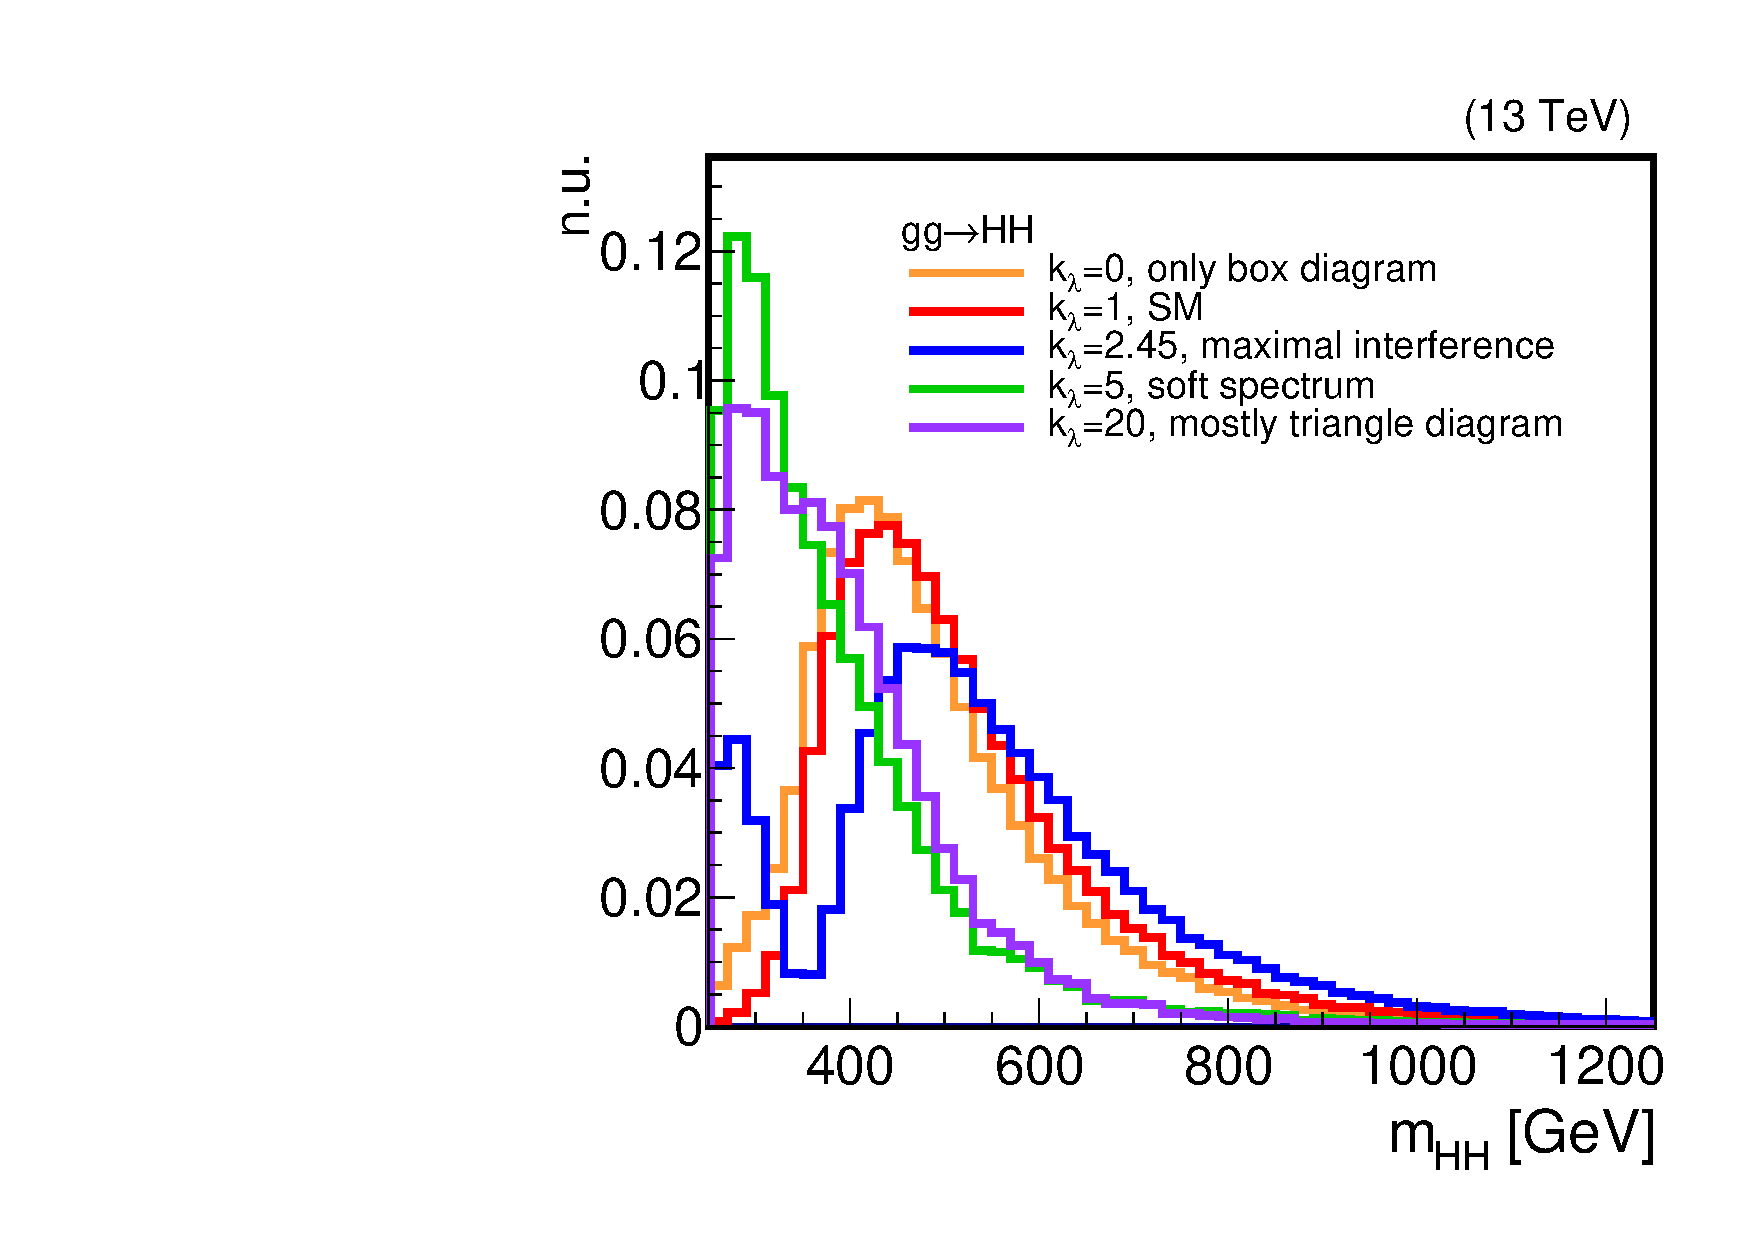
\includegraphics[width=0.50\textwidth]{Figures/HiggsPairProduction/h_gen_hh_m_ggf.pdf}}
\subfloat[]{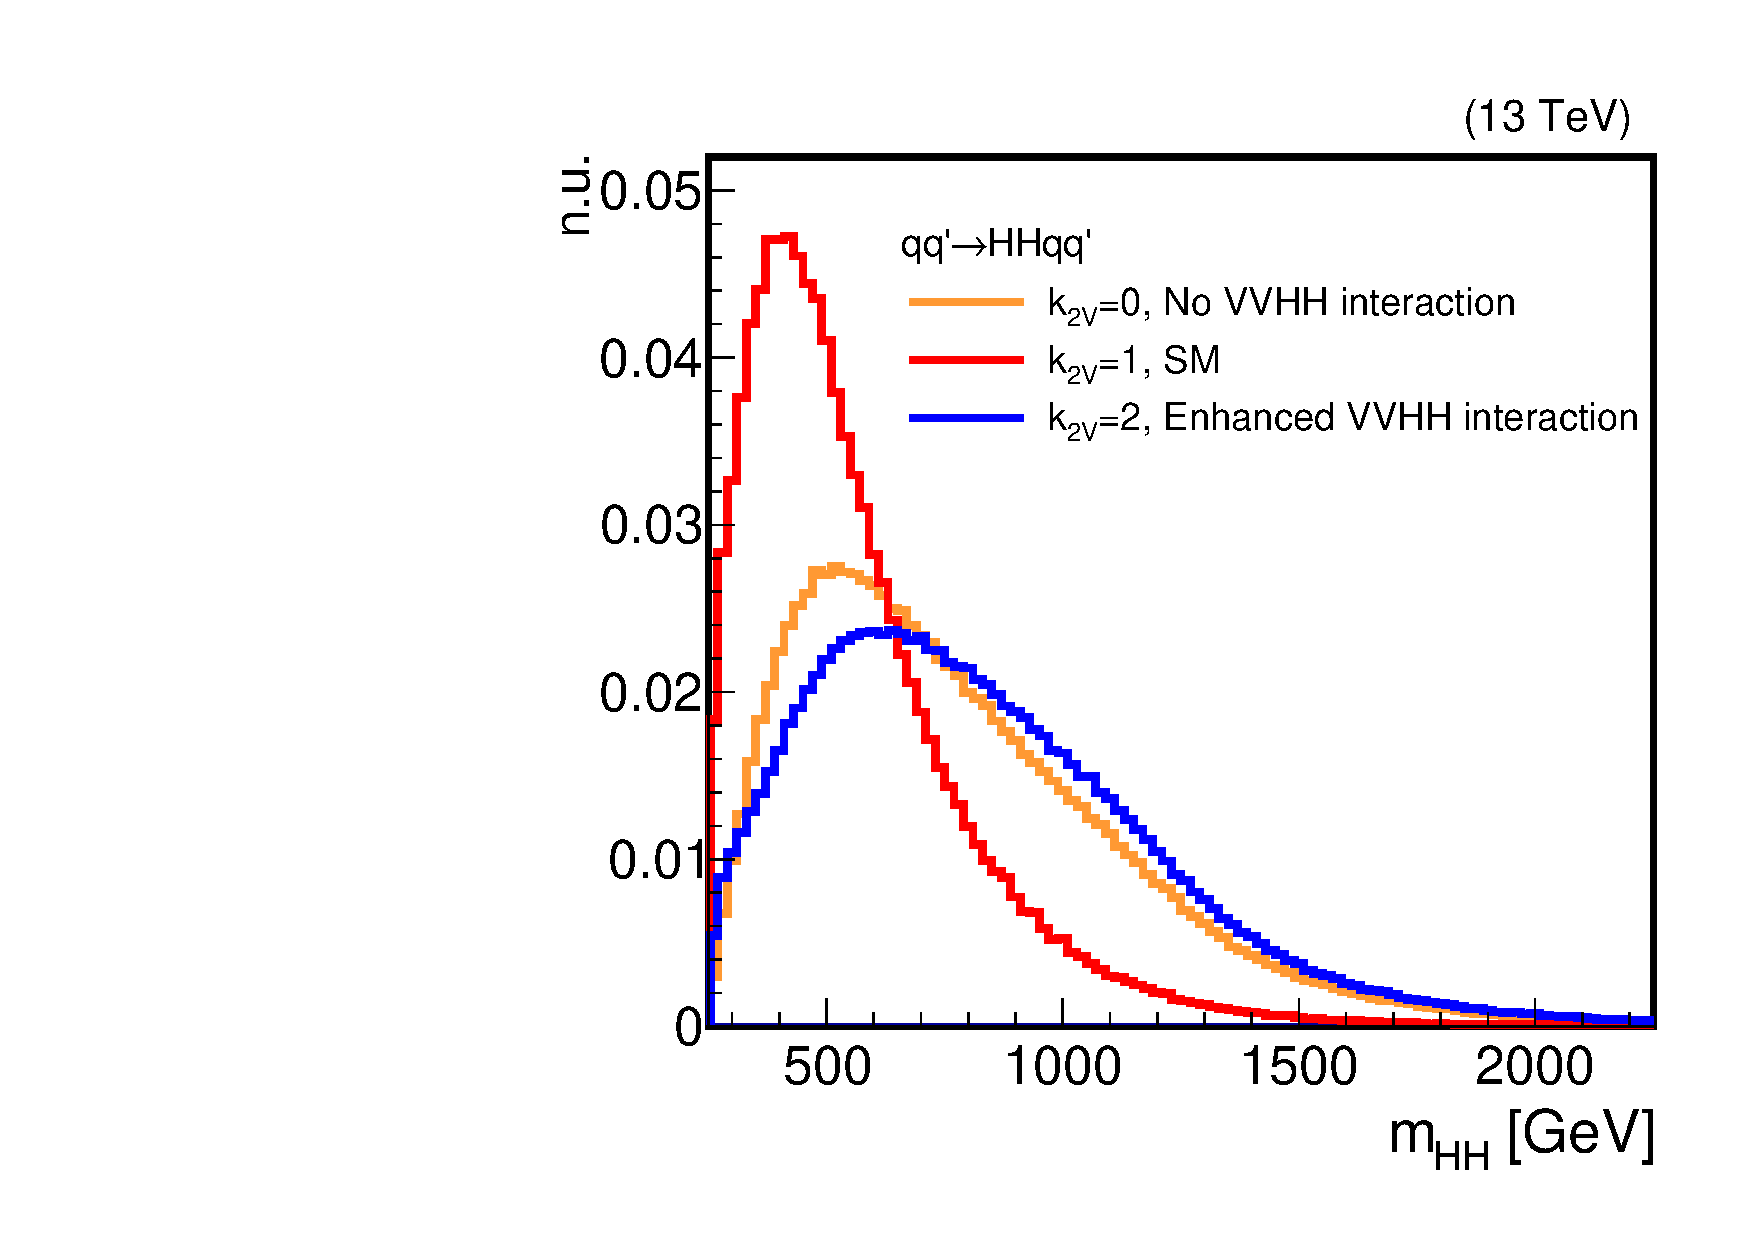
\includegraphics[width=0.50\textwidth]{Figures/HiggsPairProduction/h_gen_hh_m_vbf.pdf}}
\caption[Normalized Higgs boson pair invariant mass for different values of the coupling modifiers]{Normalized Higgs boson pair invariant mass for different values of the coupling modifiers: A) $\mathrm{\kappa_{\lambda}}$ variations in the ggF mode, and B) $\mathrm{\kappa_{2V}}$ in the VBF mode. Other Higgs couplings are set to their SM values.}
\label{fig:mhhvariation}
\end{figure}

A generalization of the BSM effects on the ggF HH production is achieved in the context of an effective field theory (EFT), where the SM Lagrangian (dimension$\leq 4$) is extended with new terms associated to dimension-6 operators~\cite{Goertz:2014qta}. The effects of these new operators represent modifications of the SM $\mathrm{y_{t}}$ and $\mathrm{\lambda_{HHH}}$ couplings with strength $\mathrm{\kappa_{\lambda}}$ and $\mathrm{\kappa_{t}=y_{t}/y_{t}^{SM}}$, and three new vertices associated to contact interactions gHH, ggHH and ttHH with coupling strengths denoted as $\mathrm{c_{g}}$, $\mathrm{c_{2g}}$ and $\mathrm{c_{2}}$, respectively. Figure~\ref{fig:cinteractions} illustrates the LO diagrams of the three EFT contact interactions. The EFT NLO accuracy model is presented in Ref.~\cite{Buchalla:2018yce}. 

\begin{figure}[htp!]
\centering
\captionsetup[subfigure]{justification=centering}
\subfloat[]{\centering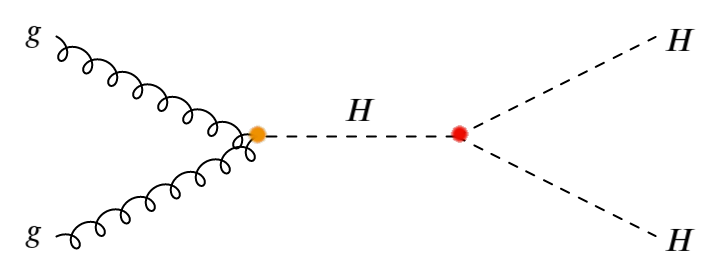
\includegraphics[width=0.35\textwidth]{Figures/HiggsPairProduction/cg.png}}
\subfloat[]{\centering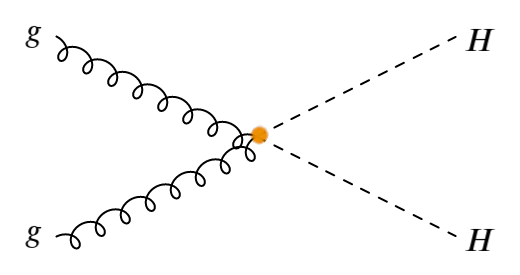
\includegraphics[width=0.29\textwidth]{Figures/HiggsPairProduction/c2g.png}}
\subfloat[]{\centering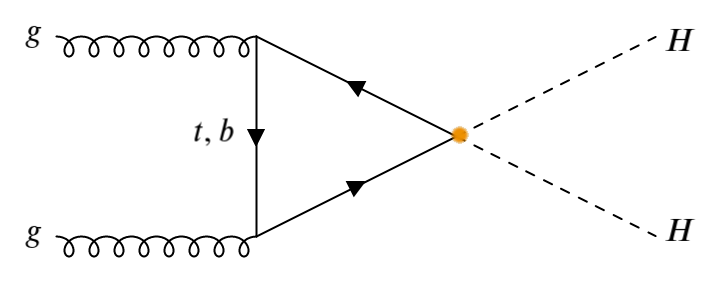
\includegraphics[width=0.35\textwidth]{Figures/HiggsPairProduction/c2.png}}
\caption[Leading order diagrams of contact interactions]{Leading order diagrams of contact interactions: A) gHH, B) ggHH and C) ttHH. The orange (red) circle represents the vertices absent in the SM (Higgs self-coupling).}
\label{fig:cinteractions}
\end{figure}

Given that is not feasible to experimentally study all possible combinations of the five EFT couplings, 12 shape benchmarks are chosen to target characteristic kinematic properties of large regions of the five-dimensional phase space by the clustering method presented in Ref.~\cite{Carvalho:2015ttv}. The coupling combination of the benchmarks are listed in Table~\ref{tab:eftcouplings} and their $\mathrm{m_{HH}}$ shapes are illustrated in Figure~\ref{fig:eftshapes}. Note that the softest spectrum corresponds to benchmark 7, whereas the hardest spectrum corresponds to benchmark 2. 

\begin{figure}[ht]
\centering
\captionsetup[subfigure]{justification=centering}
\subfloat[]{\centering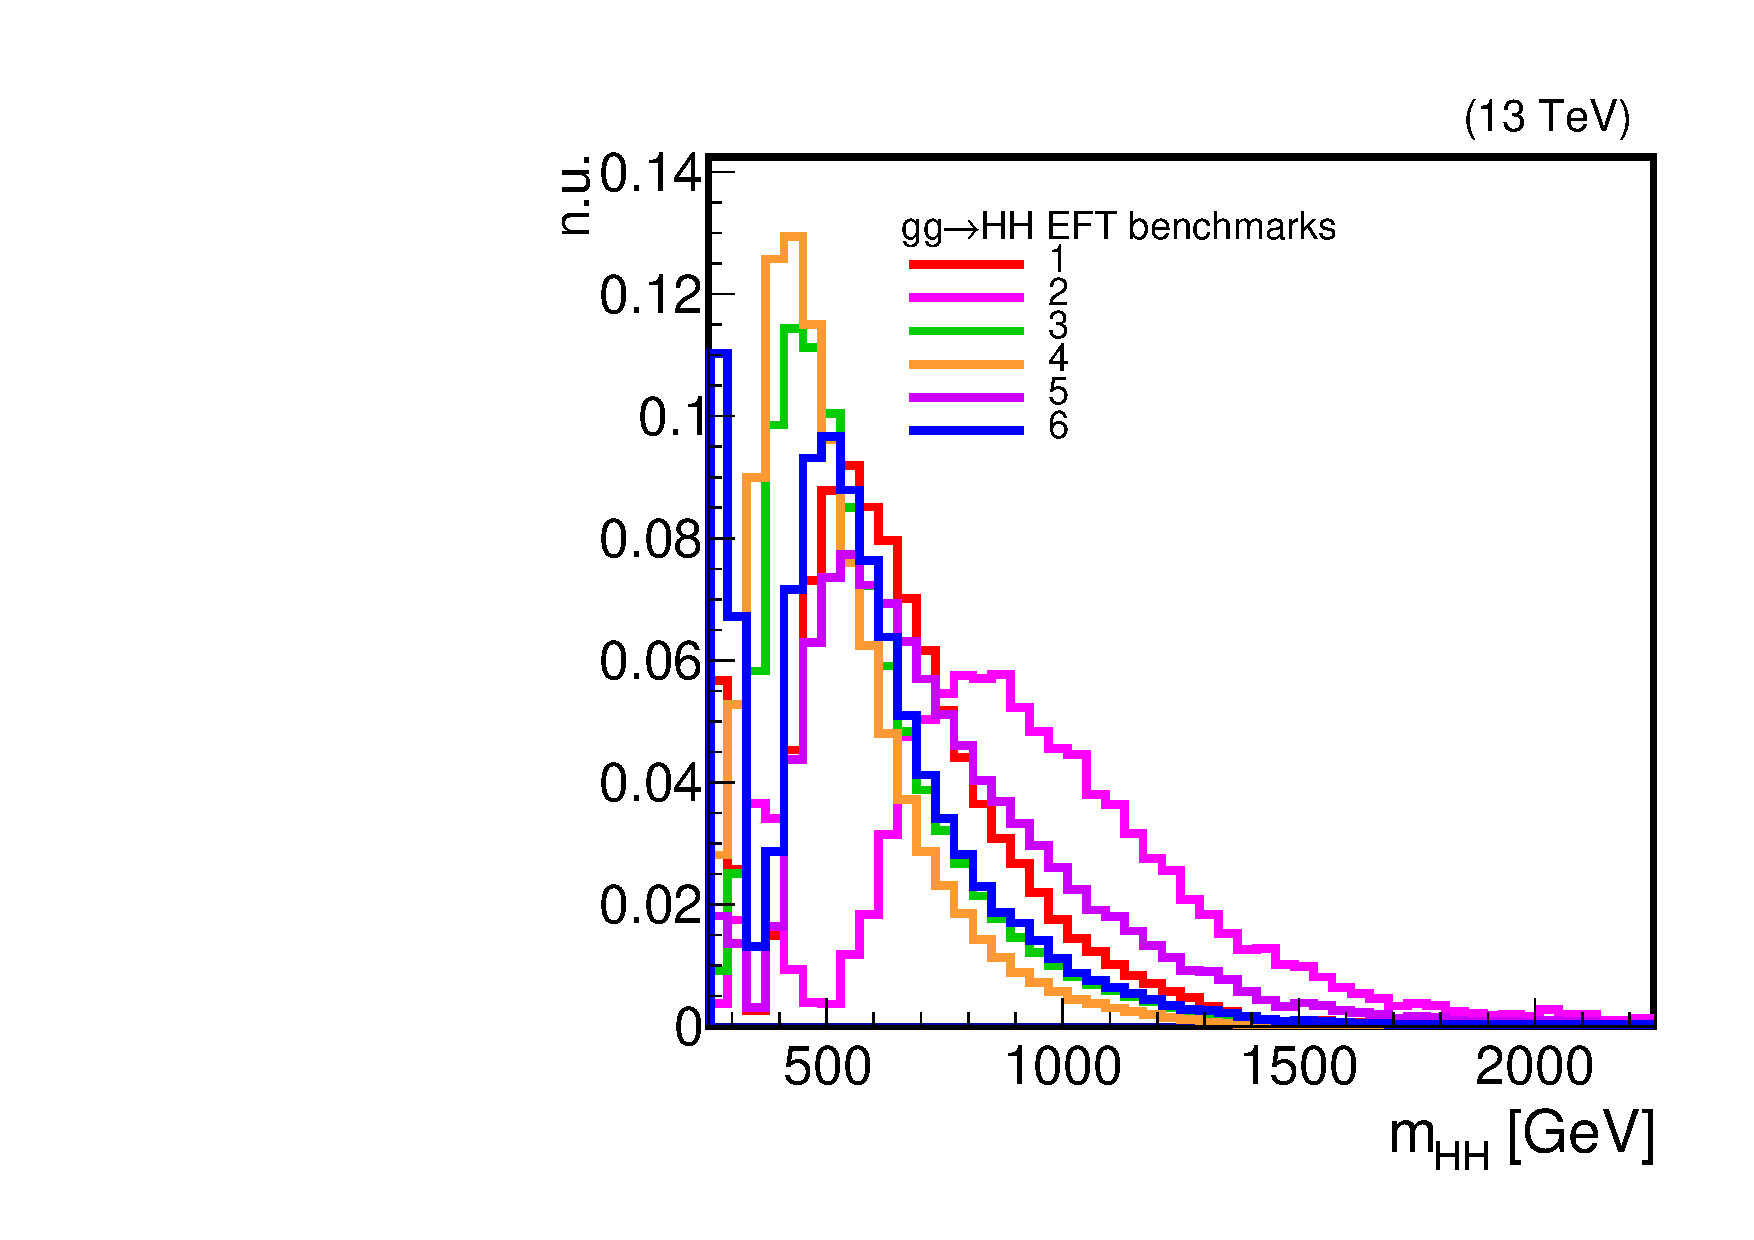
\includegraphics[width=0.42\textwidth]{Figures/HiggsPairProduction/h_gen_hh_m_eft1.pdf}}
\subfloat[]{\centering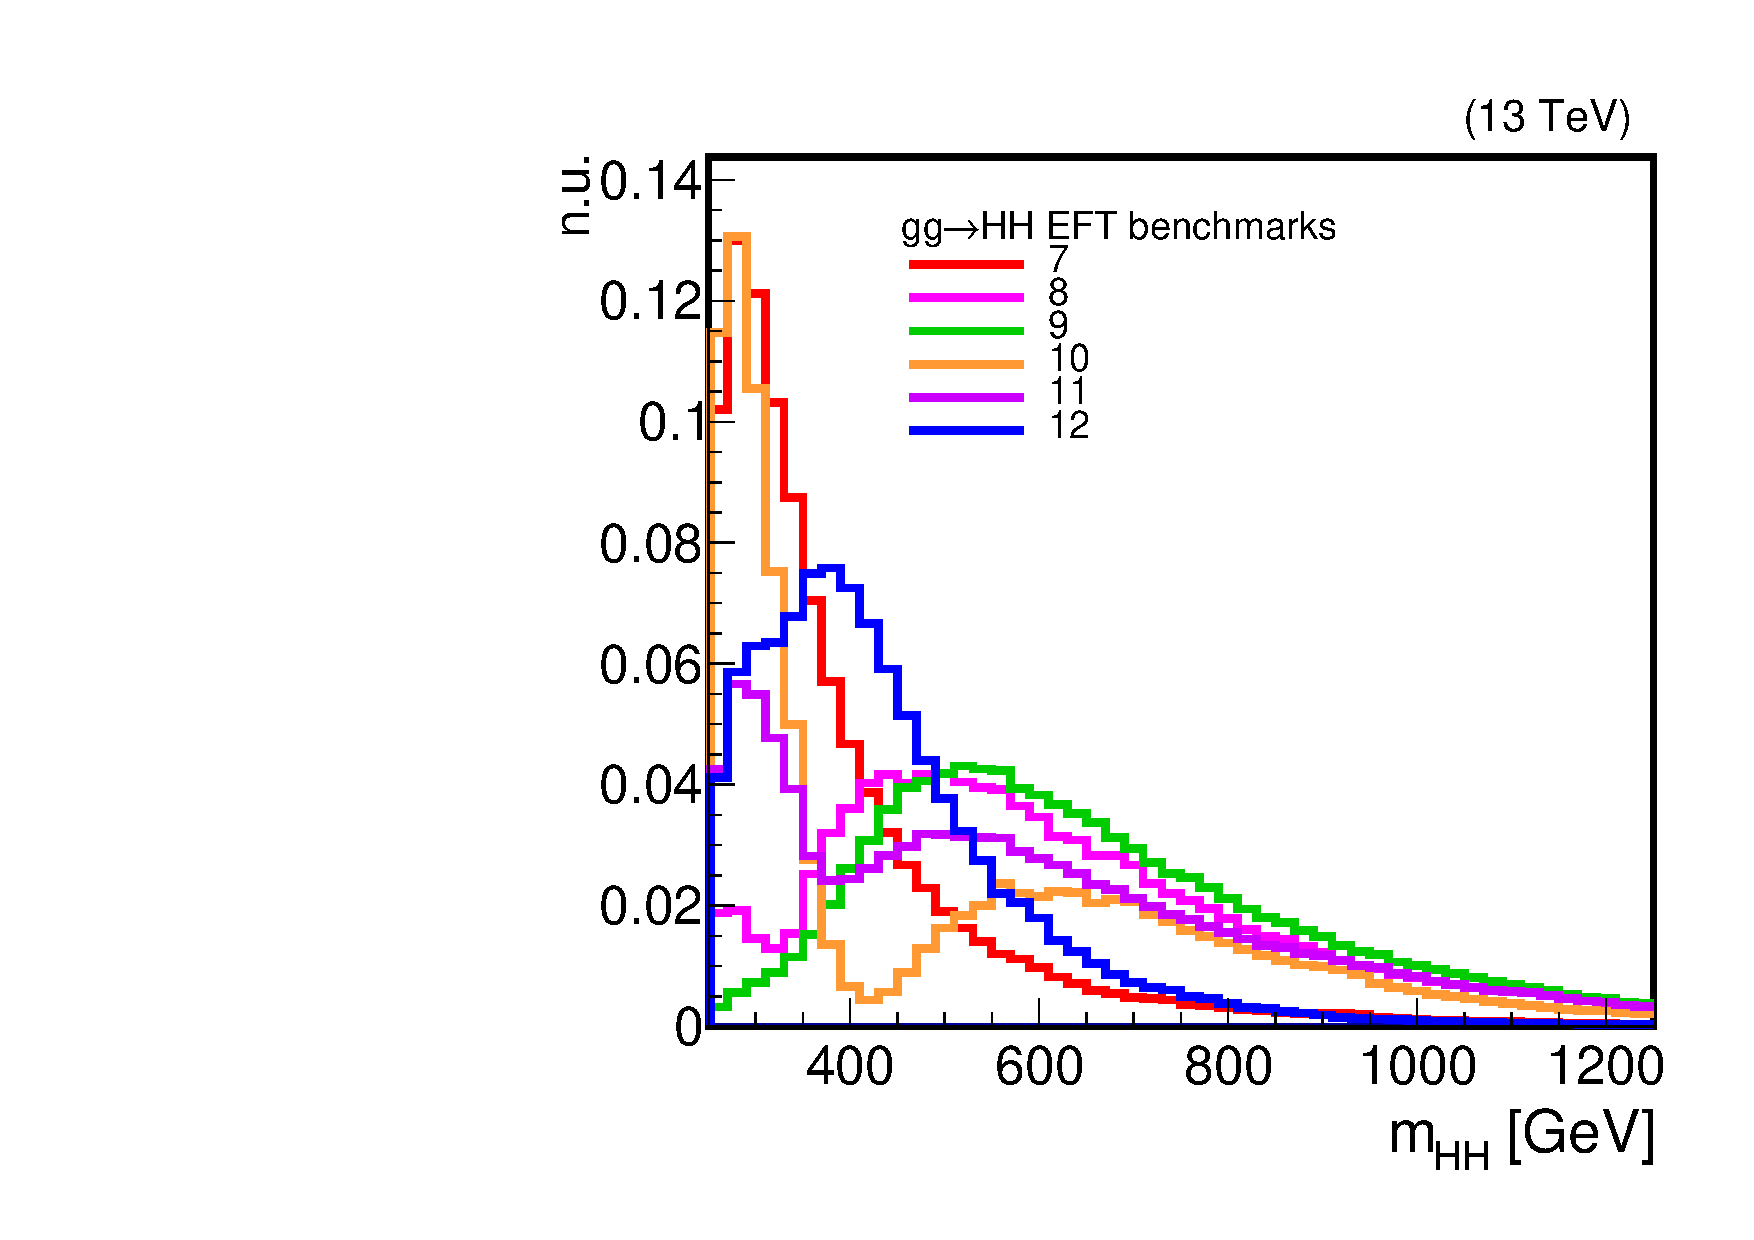
\includegraphics[width=0.42\textwidth]{Figures/HiggsPairProduction/h_gen_hh_m_eft2.pdf}}
\caption{Higgs boson pair invariant mass distribution for different leading order effective field theory (EFT) shape benchmarks: A) Nodes 1 to 6, and B) Nodes 7 to 12.}
\label{fig:eftshapes}
\end{figure}

\begin{table}[ht]
\centering
\caption[Effective field theory benchmarks for LHC searches for non-resonant Higgs boson pair production]{\label{tab:eftcouplings} Effective field theory benchmarks for LHC searches for non-resonant Higgs boson pair production via the gluon-fusion mode~\cite{Carvalho:2015ttv}.}
\begin{tabularx}{\textwidth}{XXXXXX}
\hline
Benchmark  & $\mathrm{\kappa_{\lambda}}$ &  $\mathrm{\kappa_{t}}$ &   $\mathrm{c_{2}}$ & $\mathrm{c_{g}}$  & $\mathrm{c_{g}}$ \\
\hline
1   &7.5   & 1.0  & -1.0 &  0.0 & 0.0  \\[0pt]
2   &1.0   & 1.0  &  0.5 & -0.8 & 0.6  \\[0pt]
3   &1.0   & 1.0  & -1.5 &  0.0 &-0.8  \\[0pt]
4   &-3.5  & 1.5  & -3.0 &  0.0 & 0.0  \\[0pt]
5   &1.0   & 1.0  &  0.0 &  0.8 &-1.0  \\[0pt]
6   &2.4   & 1.0  &  0.0 &  0.2 &-0.2  \\[0pt]
7   &5.0   & 1.0  &  0.0 &  0.2 &-0.2  \\[0pt]
8   &15.0  & 1.0  &  0.0 & -1.0 & 1.0  \\[0pt]
9   &1.0   & 1.0  &  1.0 & -0.6 & 0.6  \\[0pt]
10  &10.0  & 1.5  & -1.0 &  0.0 & 0.0  \\[0pt]
11  &2.4   & 1.0  &  0.0 &  1.0 &-1.0  \\[0pt]
12  &15.0  & 1.0  &  1.0 &  0.0 & 0.0  \\[0pt]
\hline
\end{tabularx}
\end{table}


\clearpage

\section{Searches for Higgs Boson Pair Production}
This section reviews the phenomenology and experimental aspects of the ongoing HH program at the LHC. First, the HH decay channels and their properties are discussed. Then, the results of the searches performed using LHC pp collision data are summarized. It ends with the most recent projections for the SM HH production at the High Luminosity LHC (HL-LHC), which were prepared in the context of the European Strategy for Particle Physics before the development of this dissertation~\cite{deBlas:2019rxi}.

\subsection{Decay Channels}
SM HH production is an elusive process to measure due to the low expected rates at the LHC. However, as mentioned before, rates and kinematics can be modified by BSM effects and potentially discovered with the current datasets. The HH signature has a rich variety of decay channels with different branching fractions depending on the two Higgs boson decays as seen in Figure~\ref{fig:hhbr}. The $\mathrm{b\overline{b}b\overline{b}}$ is the dominant decay channel with $\sim33\%$ branching fraction. Decay channels with at least one $\mathrm{H\rightarrow~bb}$ are used in searches to maintain a sizeable branching fraction.

\begin{figure}[ht!]
\centering
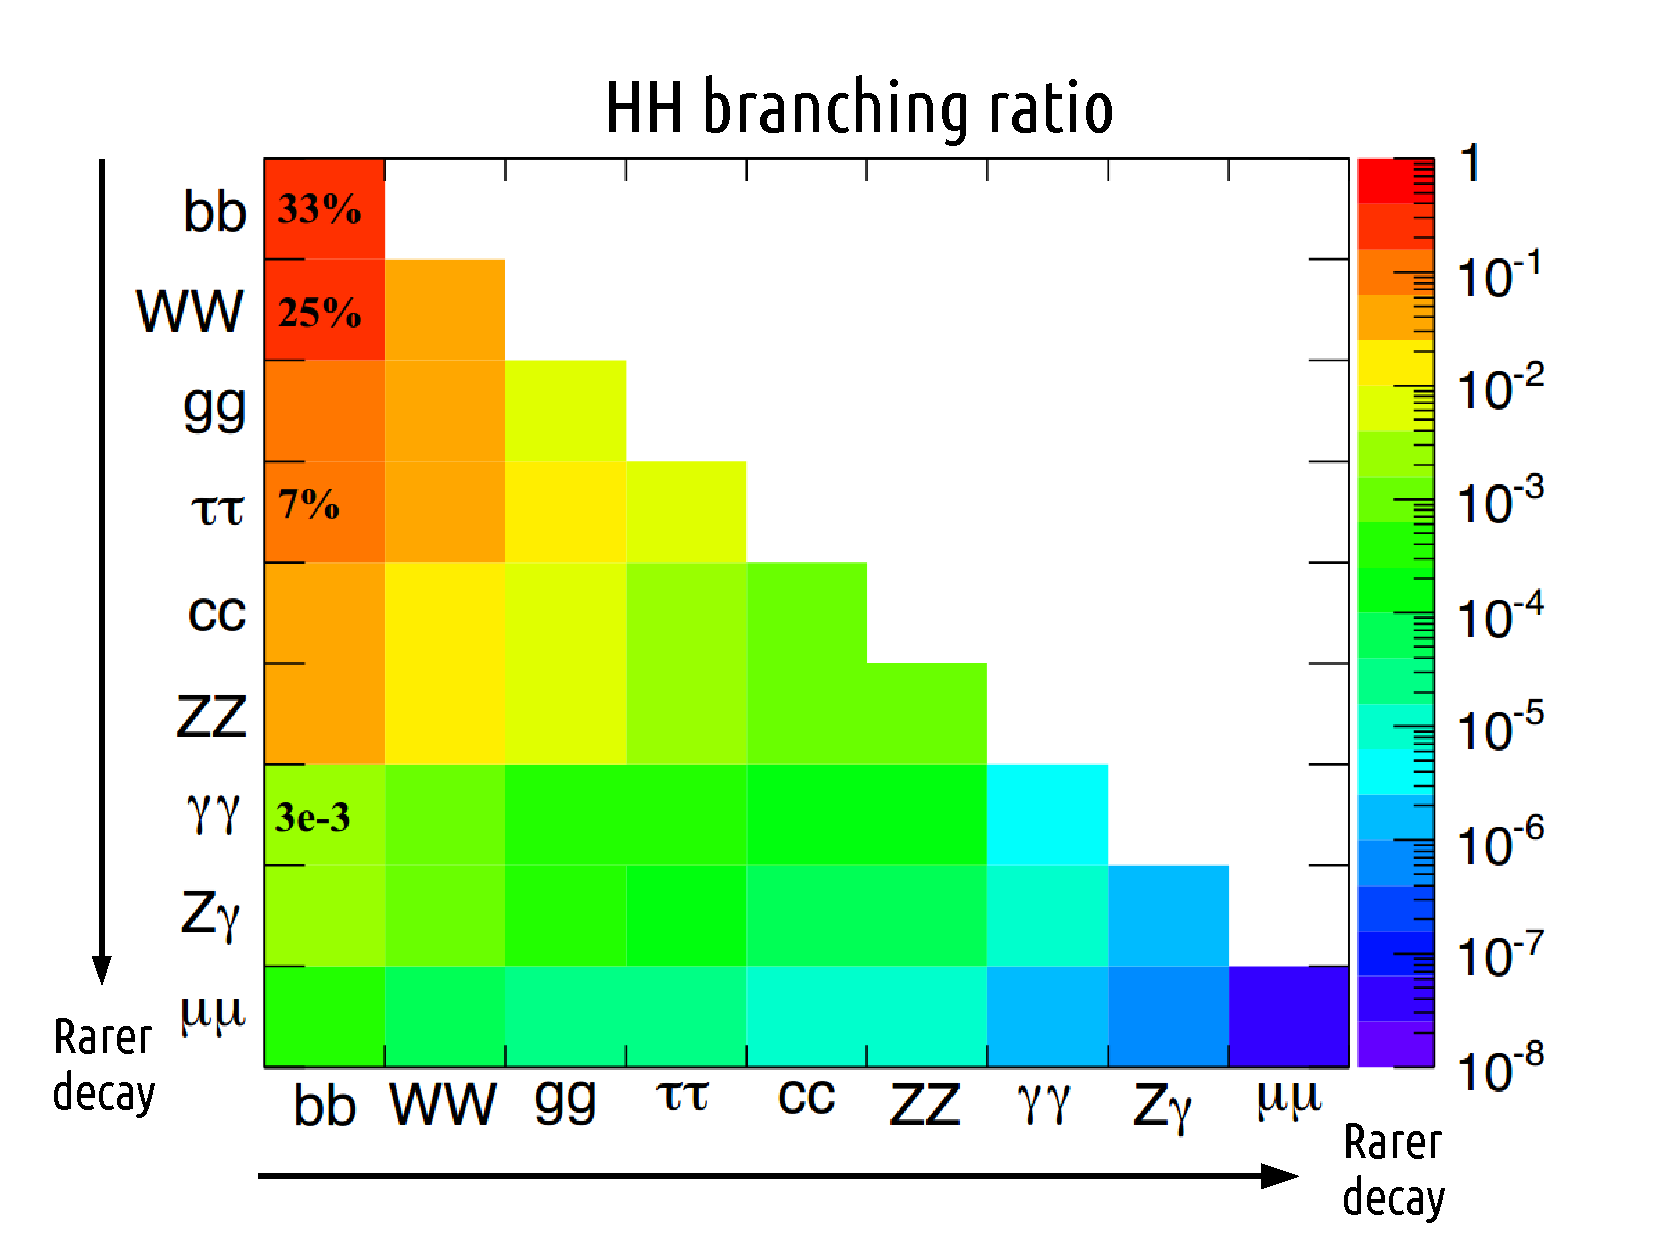
\includegraphics[width=0.63\textwidth]{Figures/HiggsPairProduction/brhh.pdf}
\caption[Higgs boson pair branching fractions assuming a Higgs mass $\mathrm{m_{H}=125~GeV}$]{Higgs boson pair branching fractions assuming a Higgs mass $\mathrm{m_{H}=125~GeV}$. The Higgs decays considered in the figure are: two bottom quarks ($\mathrm{b\overline{b}}$), two W bosons ($W^{+}W^{-}$), two gluons (gg), two tau leptons ($\tau^{+}\tau^{-}$), two charm quarks (cc), two Z bosons (ZZ), two photons ($\gamma\gamma$), a Z boson and a photon (Z$\gamma$), and two muons ($\mu\mu$).}
\label{fig:hhbr}
\end{figure}

\subsection{Experimental Status at the LHC}
The LHC has a broad experimental program exploring resonant and non-resonant HH production in multiple channels and production modes. The first results were obtained analyzing the Run-1 collision data at 8 TeV, corresponding to around 20$\mathrm{fb^{-1}}$ of integrated luminosity. ATLAS (CMS) studied the gluon fusion HH production in the  $\mathrm{b\overline{b}\gamma\gamma}$, $\mathrm{b\overline{b}\tau^{+}\tau^{-}}$, $\mathrm{b\overline{b}b\overline{b}}$ and $\gamma\gamma~W^{+}W^{-}$ ($\mathrm{b\overline{b}\gamma\gamma}$, $\mathrm{b\overline{b}\tau^{+}\tau^{-}}$ and $\mathrm{b\overline{b}b\overline{b}}$). The Run-1 ATLAS (CMS) observed combined upper limits on the SM-like HH production cross section corresponds to 70 (43) times the SM prediction, respectively. Other results in the context of BSM $\kappa_{\lambda}$ couplings and resonances were presented, but no significant excess of signal was observed~\cite{atlashhrun1comb,cmshhrun1comb}.

At the present time, CMS and ATLAS experts are exploring searches with more production modes and new decay channels by analyzing the full Run-2 dataset collected at 13 TeV. While those results are being finished, both experiments already released a very comprehensive study of direct searches via the ggF mode by combining the results obtained in several channels using partial Run-2 dataset~\cite{atlascomb,cmscomb}. The ATLAS (CMS) dataset was collected during the 2015-2016 (2016) operations with an integrated luminosity of 27.1--36.1 (35.9) $\mathrm{fb^{-1}}$. The ATLAS (CMS) channels used in the combination are the following: $\mathrm{b\overline{b}\gamma\gamma}$~\cite{bbggatlas}, $\mathrm{b\overline{b}\tau^{+}\tau^{-}}$~\cite{bbttatlas1}, $\mathrm{b\overline{b}b\overline{b}}$~\cite{bbbbatlas}, $\mathrm{W^{+}W^{-}W^{+}W^{-}}$~\cite{atlaswwww} and $\gamma\gamma\mathrm{W^{+}W^{-}}$~\cite{atlasggww} ($\mathrm{b\overline{b}b\overline{b}}$ boosted~\cite{bbbbcmsr2} and resolved~\cite{bbbbcmsnr,bbbbcmsr1}, $\mathrm{b\overline{b}}\gamma\gamma$~\cite{bbggcms}, $\mathrm{b\overline{b}}\tau^{+}\tau^{-}$~\cite{bbttcms1,bbttcms2}, $\mathrm{b\overline{b}VV}$~\cite{cmsbbvv}). In addition, both experiments studied indirect $\kappa_{\lambda}$ constraints from single Higgs searches~\cite{cmsrun2mes,atlasindirecthh}.

The ATLAS (CMS) combination set an observed limit on the SM production cross section at 6.9 (22) times the SM prediction. The observed allowed $\kappa_{\lambda}$ interval at 95\% CL ranges from -5.0 (-11.8) to 12.0 (18.8). Results on EFT benchmarks were also presented. Furthermore, both experiments presented results on resonant searches for new particles with Spin-0 and Spin-2 in the mass range between 250 GeV and 3 TeV. However, no statistically significant excess of resonant events were observed, and 95\% CL limits on the production cross section of new resonances decaying into Higgs pairs were provided. In addition, the ATLAS (CMS) results from single Higgs searches presented the 95\% CL allowed $\kappa_{\lambda}$ interval from -3.2 (-3.5) to 11.9 (14.5).

Excluding the results of this dissertation, several Run-2 HH non-resonant analyses have been performed. The ATLAS experiment has presented the study of the ggF production mode in the $\mathrm{b\overline{b}\gamma\gamma}$~\cite{atlasfullrun2bbgg}, $\mathrm{b\overline{b}\tau^{+}\tau^{-}}$~\cite{atlasrun2bbtt},  and $\mathrm{b\overline{b}W^{+}W^{-}(\ell\nu\ell\nu)}$~\cite{atlasfullrun2bbwwdilep} channels, whereas the CMS experiment has explored the same mode in the $\mathrm{b\overline{b}\gamma\gamma}$~\cite{cmsfullrun2bbgg} and $\mathrm{b\overline{b}ZZ(4\ell)}$~\cite{cmsbbzz4l} channels. Moreover, the VBF production mode has been explored by the ATLAS experiment in the $\mathrm{b\overline{b}b\overline{b}}$~\cite{atlasfullrun2vbf4b}, whereas CMS experiment has done it in the $\mathrm{b\overline{b}\gamma\gamma}$~\cite{cmsfullrun2bbgg} channel, and the $\mathrm{b\overline{b}b\overline{b}}$ channel studying highly Lorentz-boosted Higgs bosons~\cite{cmsrun2boostedbbbb}.  Once the main decay channels are analyzed, then a full Run-2 HH combination will be performed. In addition, full Run-2 resonant searches have also been performed in ATLAS~\cite{atlasfullrun2bbgg,atlasrun2bbtt,atlasfullrun2vbf4b} and CMS~\cite{cmsrun2resboostbbbb,cmsrun2resboostbbww}. 

The best LHC results on non-resonant HH production are obtained from the currently finalized full Run-2 analyses. From the ATLAS combination of the results of the $\mathrm{b\overline{b}\gamma\gamma}$ and $\mathrm{b\overline{b}\tau^{+}\tau^{-}}$ channels, the current observed limit on the SM-like HH production cross section is 3.1 times the SM expectation, and the observed allowed $\kappa_{\lambda}$ interval at 95\% CL is from -1.0 to 6.6 as presented in Figure~\ref{fig:hhbestresults} A)~\cite{ATLAS-CONF-2021-052}. Furthermore, the current observed limit on VBF production cross section is 225 times the SM prediction by the CMS search in the $\mathrm{b\overline{b}\gamma\gamma}$ channel. Finally, the observed allowed interval of the $\kappa_{2V}$ modifier is from 0.6 to 1.4, corresponding to the search in the $\mathrm{b\overline{b}b\overline{b}}$ channel with highly Lorentz-boosted Higgs bosons (illustrated in Figure~\ref{fig:hhbestresults}~B))~\cite{cmsrun2boostedbbbb}.

The search sensitivity of the HH searches depends on the rates (production cross section and branching ratio), selection efficiencies, level of background contamination and mass resolution. The HH signal is reconstructed by the ATLAS and detectors from objects associated to the final state particles. These objects are b-quark hadronic jets (b) or `b-jets', light-quark jets (j), hadronic or leptonic $\tau$ leptons, muons and electrons ($\ell$), photons ($\gamma$), and missing transverse energy (MET) if neutrinos ($\nu$) are present. As the quality of the object reconstruction has a direct impact on the HH signal identification, ATLAS and CMS have developed algorithms to improve it. For instance, there are dedicated jet identification algorithms based on machine learning to improve the reconstruction of the $\mathrm{H\rightarrow~b\overline{b}}$ decay from two small-radius b-jets or a large-radius jet (if H has a large Lorentz boost)~in CMS~\cite{cmsbtag1,cmsbtag2} and ATLAS~\cite{atlasbtag1,atlasbtag2}. Moreover, there are multivariate regression algorithms to correct the reconstructed b-jet energy from the unmeasured energy associated neutrinos inside the b-jet from semileptonic B hadron decays~(e.g. see Ref.\cite{cmsbreg}).

\begin{figure}[ht!]
\centering
\captionsetup[subfigure]{justification=centering}
\subfloat[]{\centering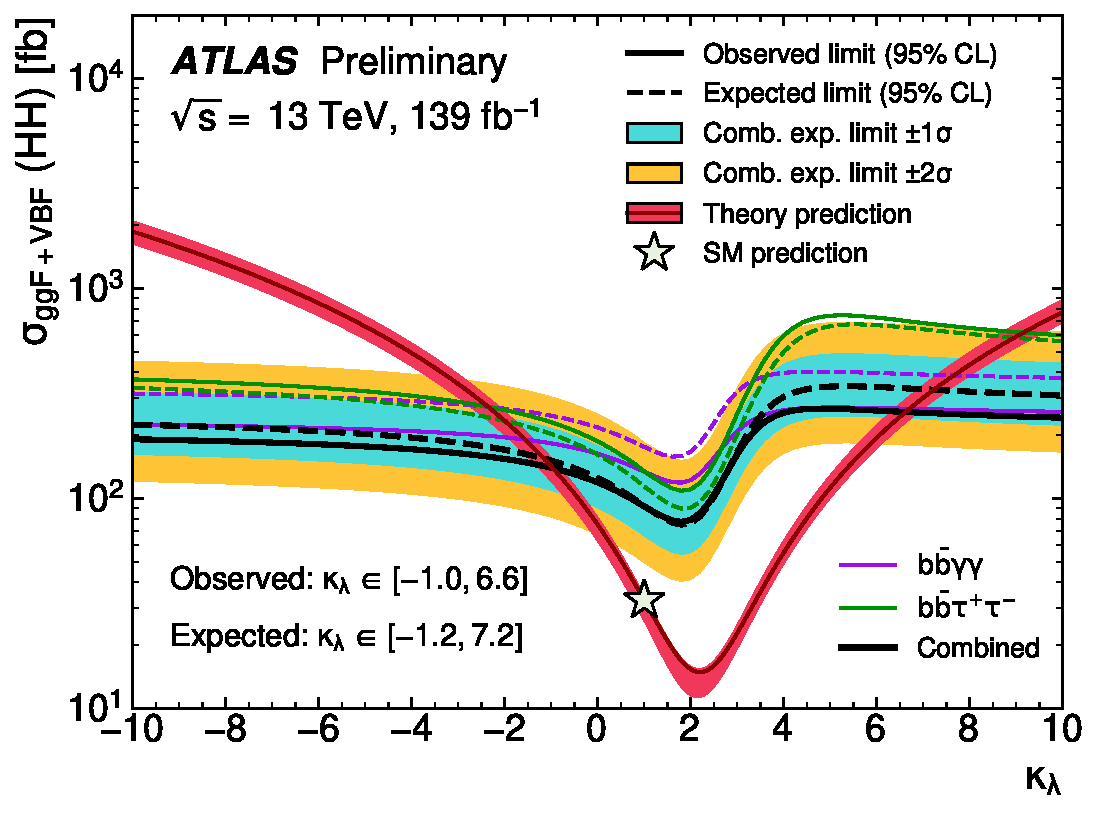
\includegraphics[width=0.45\textwidth]{Figures/HiggsPairProduction/bestatlashh.pdf}}
\subfloat[]{\centering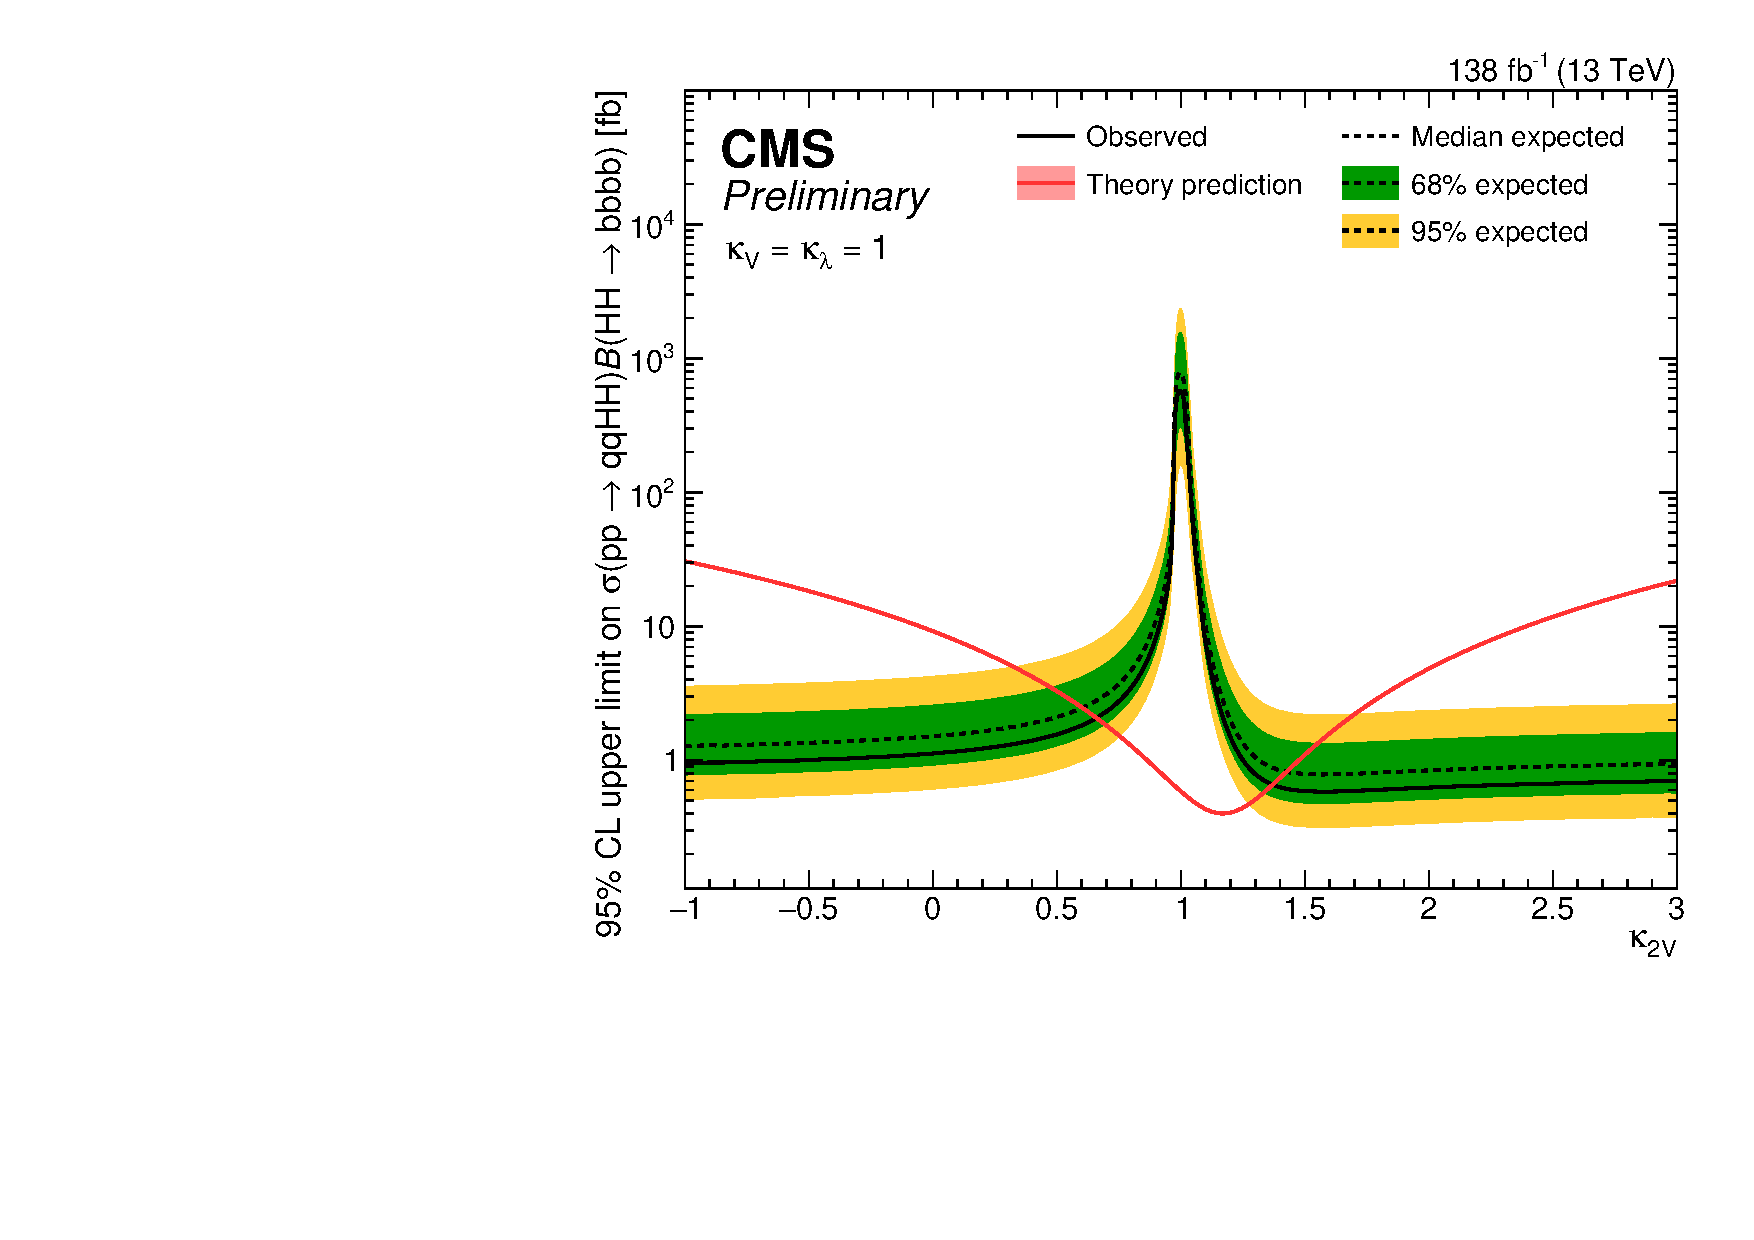
\includegraphics[width=0.42\textwidth]{Figures/HiggsPairProduction/bestk2vresult.pdf}}
\caption[95\% CL observed and expected upper limits on the Higgs boson pair production cross section as function of the coupling modifiers]{95 \% CL observed and expected upper limits on the Higgs boson pair production cross section as function of the coupling modifiers. A) Gluon fusion and vector boson fusion production cross section as a function of $\kappa_{\lambda}$~\cite{ATLAS-CONF-2021-052}, B) Vector boson fusion cross section as a function of $\kappa_{2V}$~\cite{cmsrun2boostedbbbb}.}
\label{fig:hhbestresults}
\end{figure}

There are three crucial HH decay channels based on the experience gained in the Run-1 and 2016 analyses: $\mathrm{b\overline{b}\gamma\gamma}$, $\mathrm{b\overline{b}\tau^{+}\tau^{-}}$ and $\mathrm{b\overline{b}b\overline{b}}$. Their properties and experimental aspects are summarized in the following points:
\begin{itemize}
\item $\mathrm{b\overline{b}\gamma\gamma}$: This channel has a small branching ratio ($\sim0.3\%$) but a resonant signature over smoothly falling small background from multi-jet + photons ($\mathrm{N\gamma + jets,~N=1,2}$) processes. There is also a background contribution from single Higgs production ($\mathrm{H\rightarrow\gamma\gamma + jets}$) production. It is very sensitive for searches at low $\mathrm{m_{HH}}$ mass. The observables used for signal identification are based on the reconstructed masses of the two Higgs bosons taking advantage of the excellent di-photon mass resolution, as illustrated in Figure~\ref{fig:hhsearchobservables} A).
\item $\mathrm{b\overline{b}\tau^{+}\tau^{-}}$: This decay channel has an intermediate branching ratio but challenging background from top-quark pair, Drell-Yan (Z/$\gamma$ + jets) and multi-jet production. Searches are performed using the $\mathrm{H\rightarrow~\tau^{+}\tau^{-}}$ final states with two hadronic decays ($\tau_{had}\tau_{had}$), one hadronic and one leptonic decays ($\mathrm{\tau_{had}\tau_{\ell=e,\mu}}$). The signal identification is performed using observables based on Higgs pair mass and machine learning algorithms, as seen in Figure~\ref{fig:hhsearchobservables} B).
\item $\mathrm{b\overline{b}b\overline{b}}$: This channel is the focus of this dissertation. It benefits from the largest branching fraction. However, there is an overwhelming amount of multi-jet background processes, which make it very hard to measure it. Consequently, these searches relies on the good performance of the jet flavor tagging algorithms and a precise measurement of the background from data. The signal identification discriminants are based on machine learning and the Higgs pair mass, e.g. in Figure~\ref{fig:hhsearchobservables} C). This is the most sensitive channel for searches at high $\mathrm{m_{HH}}$ mass. 
\end{itemize}

\begin{figure}[ht!]
\centering
\captionsetup[subfigure]{justification=centering}
\subfloat[]{\centering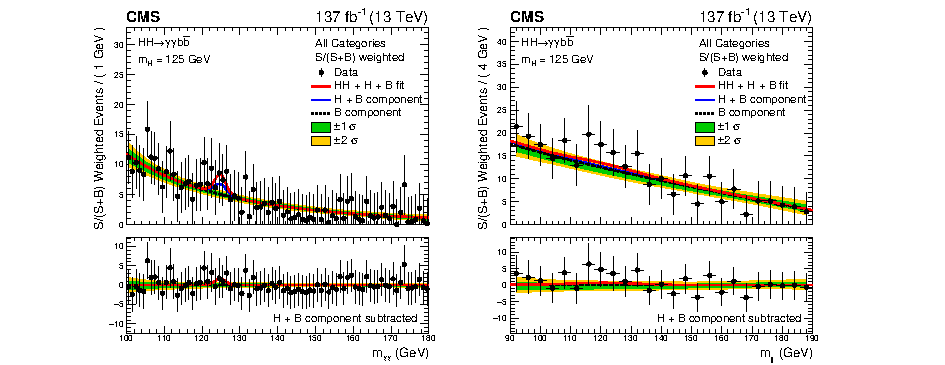
\includegraphics[width=1.0\textwidth]{Figures/HiggsPairProduction/bbggobservables.pdf}}\\
\subfloat[]{\centering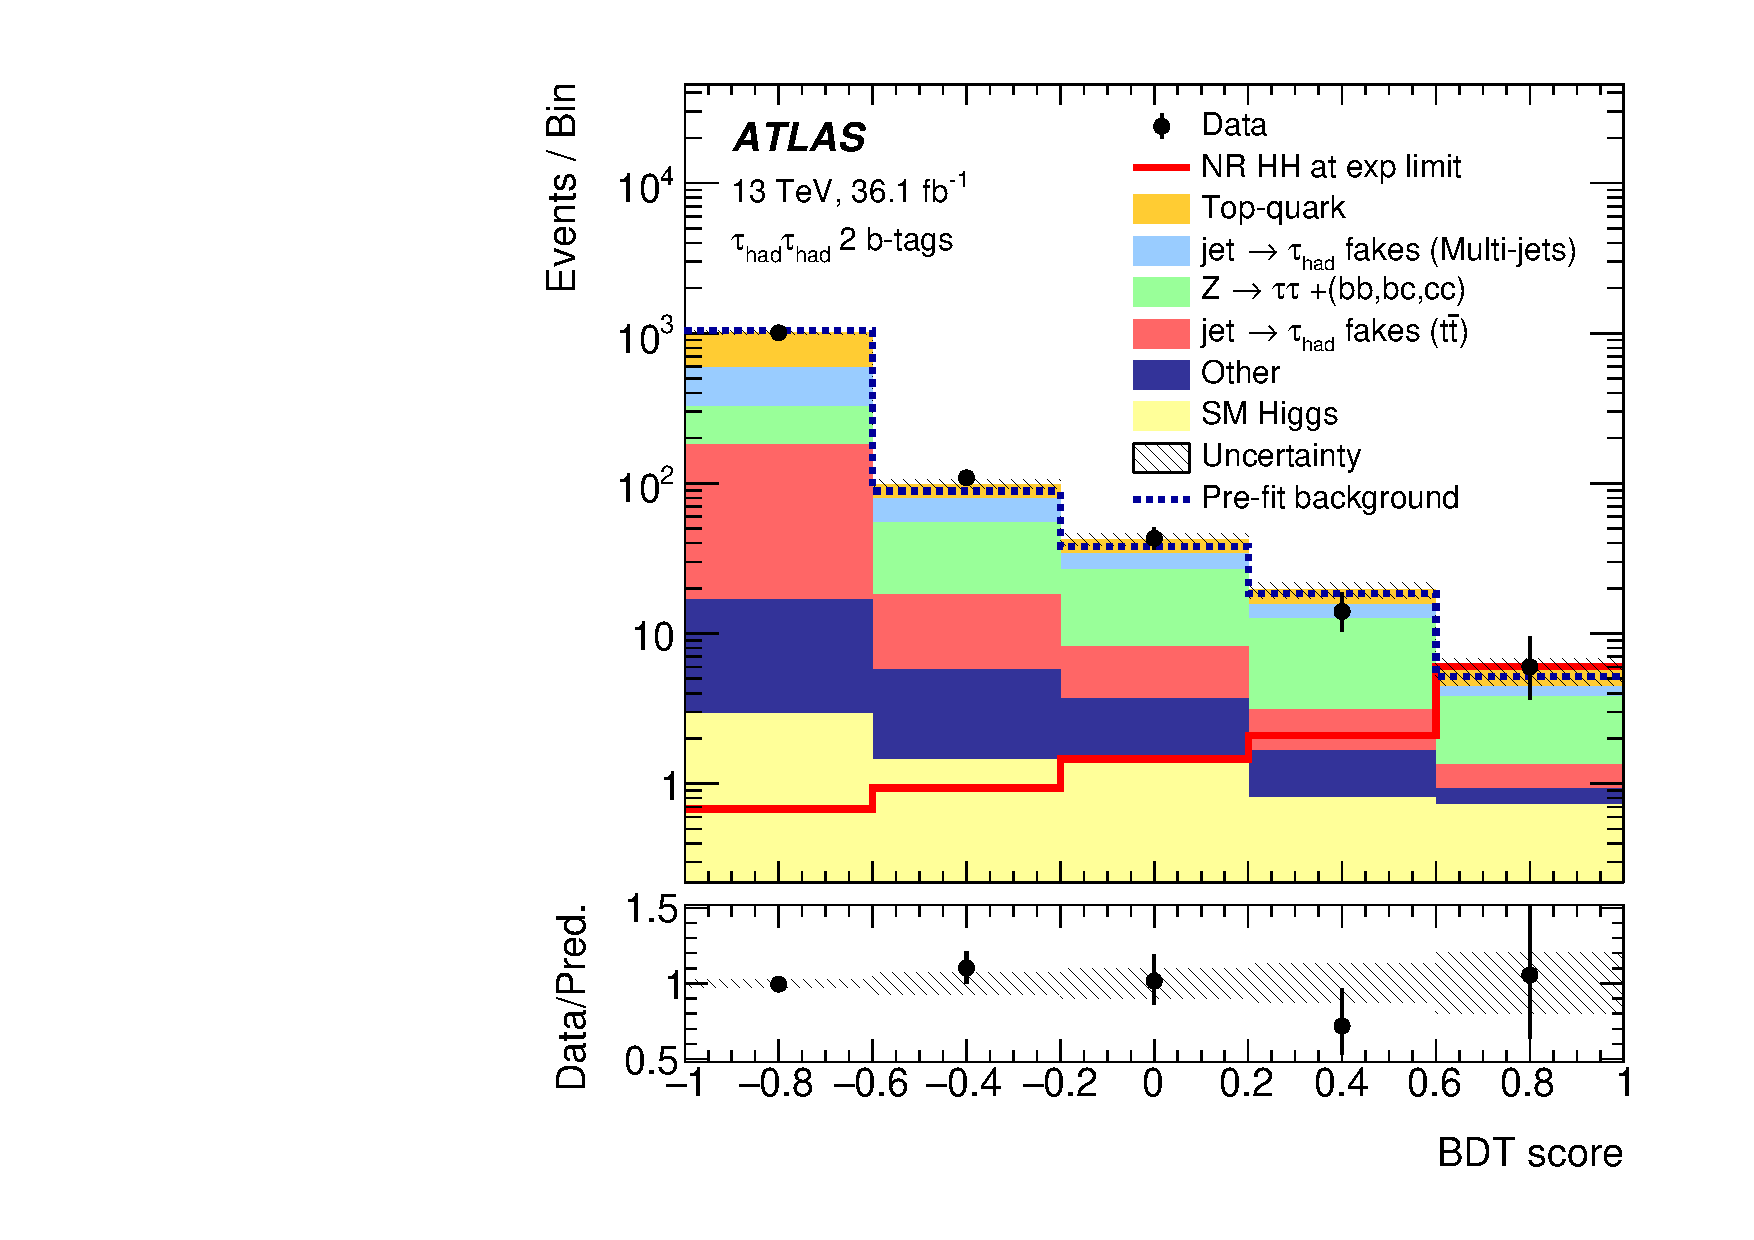
\includegraphics[width=0.40\textwidth]{Figures/HiggsPairProduction/bbtautauobservable.pdf}}
\subfloat[]{\centering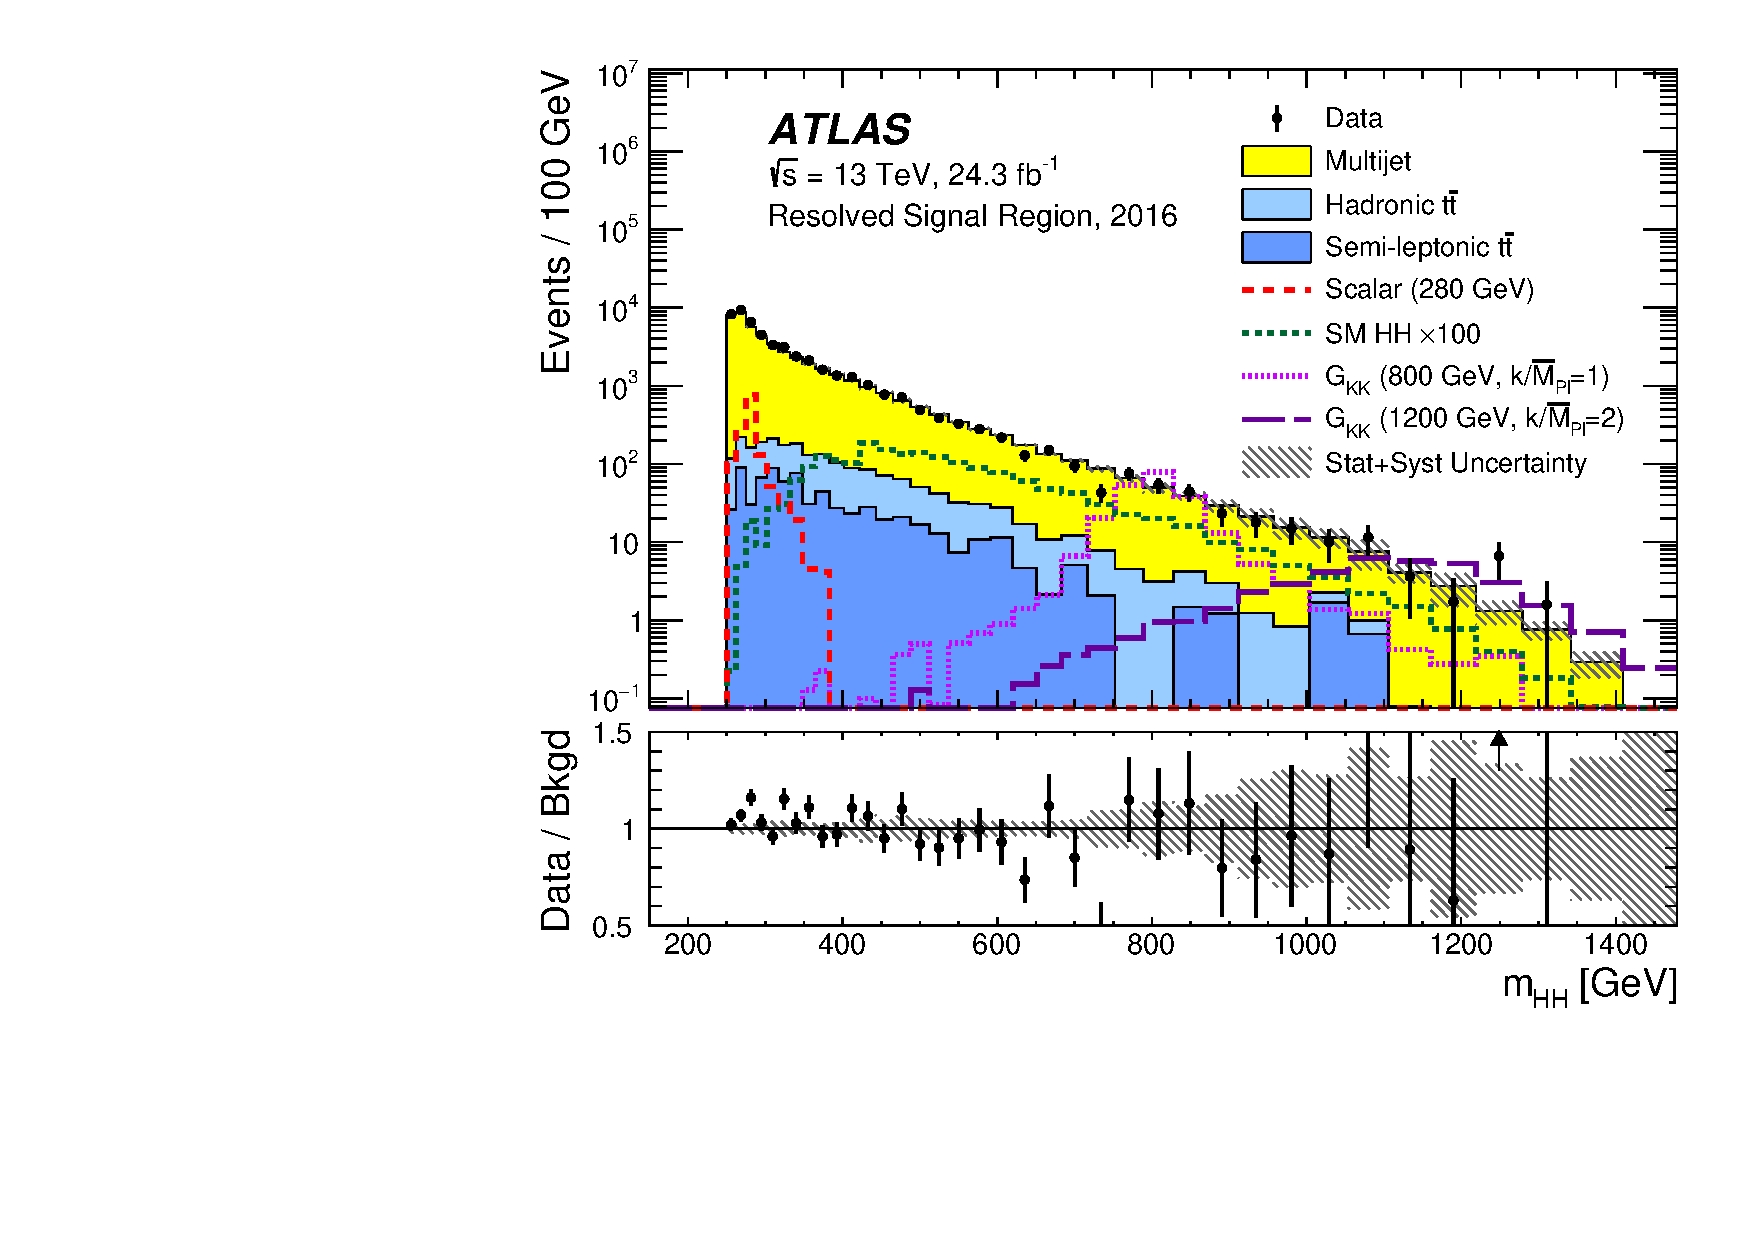
\includegraphics[width=0.46\textwidth]{Figures/HiggsPairProduction/bbbbobservable.pdf}}
\caption[Signal observables used in searches for HH production]{Signal observables used in searches for HH production. A) di-photon and bottom-quark pair distributions used in the last search for $\mathrm{HH\rightarrow~b\overline{b}\gamma\gamma}$ by CMS~\cite{cmsfullrun2bbgg}, B) Boosted decision trees (BDT) distribution used in the last search for $\mathrm{HH\rightarrow~b\overline{b}\tau^{+}\tau^{-}}$ by ATLAS~\cite{bbttatlas1}, C) Higgs boson pair mass distribution used in the last search for $\mathrm{HH\rightarrow~b\overline{b}b\overline{b}}$ by ATLAS~\cite{bbbbatlas}.}
\label{fig:hhsearchobservables}
\end{figure}

\subsection{Future Prospects at the High Luminosity LHC}
The LHC is currently under its second long shutdown (LS2) and preparing for the Run-3 data-taking program (2022-2025). Next, CMS and ATLAS will upgrade their detectors, trigger and data acquisition systems during a third long shutdown (LS3) to prepare themselves for the ultimate configuration of the LHC, the so-called High Luminosity LHC (HL-LHC). Each experiment is expected to collect a dataset of pp collisions at 14 TeV of center-of-mass energy within 10 years of the HL-LHC operation, corresponding to 3000--4000 $\mathrm{fb^{-1}}$ of integrated luminosity ($\sim20$ times more than in Run-2). More details are discussed in Chapter~\ref{chapter:apparatus}.  

The analysis of these large dataset will be crucial for a potential measurement of the SM HH production and the Higgs boson self-coupling $\mathrm{\lambda_{HHH}}$. In consequence, ATLAS and CMS experiments have already started to study what the challenges and developments needed are to reach that goal in the future. Both have presented the most recent projections of the searches for this elusive process at the HL-LHC based on the current analysis strategies on the gluon fusion mode and assuming an expected integrated luminosity of 3000 $\mathrm{fb^{-1}}$~\cite{atlasprojections,cmsprojections}. In these studies, the channels considered by ATLAS (CMS) are  $\mathrm{b\overline{b}\gamma\gamma}$, $\mathrm{b\overline{b}\tau^{+}\tau^{-}}$ and  $\mathrm{b\overline{b}b\overline{b}}$  ($\mathrm{b\overline{b}\gamma\gamma}$, $\mathrm{b\overline{b}\tau^{+}\tau^{-}}$, $\mathrm{b\overline{b}b\overline{b}}$, $\mathrm{b\overline{b}VV(\ell\ell\nu\nu)}$ and $\mathrm{b\overline{b}ZZ(4\ell)}$). In particular, the $\mathrm{b\overline{b}b\overline{b}}$ channel studies show that its main challenges will be our capability to have online triggers with high signal selection efficiency and model the multi-jet background events with high precision. 
\begin{table}[htb]
\centering
\caption[ATLAS and CMS expected significance (in standard deviation) for SM Higgs pair production in different channels at the HL-LHC]{\label{tab:significance} ATLAS and CMS expected significance (in standard deviation) for SM Higgs pair production in different channels at the HL-LHC~\cite{yellowreport}. }
\begin{tabularx}{\textwidth}{XXXX}
\hline
Channel                                     & ATLAS  &      CMS  \\
\hline
$\mathrm{b\overline{b}b\overline{b}}$       & 0.61   &  0.95     \\[0pt]
$\mathrm{b\overline{b}\tau^{+}\tau^{-}}$            & 2.1    &  1.4      \\[0pt]
$\mathrm{b\overline{b}\gamma\gamma}$        & 2.0    &  1.8      \\[0pt]
$\mathrm{b\overline{b}VV(\ell\ell\nu\nu)}$  & --     &  0.56     \\[0pt]
 $\mathrm{b\overline{b}ZZ(4\ell)}$          & --     &  0.37     \\[0pt]
Combination                                 & 3.0    &  2.6      \\[0pt]
\hline
\end{tabularx}
\end{table}

According to the projections, the ATLAS (CMS) expected significance yields a value of 3.0 (2.6) standard deviations from the combination of its individual channels.  The expected significance per channel and per experiment are summarized in Table~\ref{tab:significance}. In particular, for the $\mathrm{b\overline{b}b\overline{b}}$ channel, the ATLAS (CMS) expected significance is around 0.61 (0.95) standard deviations. Furthermore, the measurement of negative-log-likelihood as a function of the $\kappa_{\lambda}$ coupling modifier, assuming that the SM process occurs, is presented by channel in Figure~\ref{fig:coklprojection} A). From the combination of the likelihood scans in different channels, the ATLAS (CMS) $\kappa_{\lambda}$ measurement is expected to be $1^{+0.90}_{-0.75}$ ($1^{+0.90}_{-0.65}$) at 68\% CL.

The combination of the ATLAS and CMS HL-LHC projections is reported in ref.~\cite{yellowreport}. The combined significance yields a value of 4.0 standard deviations. The combined likelihood scan is presented in Figure~\ref{fig:coklprojection} B). From combined likelihood, the expected coupling measurement is $\kappa_{\lambda}=1^{+0.50}_{-0.48}$ at 68\% CL. The results of these projections show that we may achieve evidence for the SM HH production process and measure the Higgs self-coupling at around 50\% level precision. However, further detector and algorithm developments (e.g. triggering) are expected. These projections are conservative because larger datasets would enable more sophisticated analyses, which can boost the performance. Therefore, the actual results may be better than this projection. Dedicated future colliders will be needed to push further the precision of these measurements, e.g. $e^{+}e^{-}$ colliders (ILC and FCC-ee) at center-of-mass energies above 0.5 TeV~\cite{deBlas:2019rxi}.
\begin{figure}[ht!]
\centering
\captionsetup[subfigure]{justification=centering}
\subfloat[]{\centering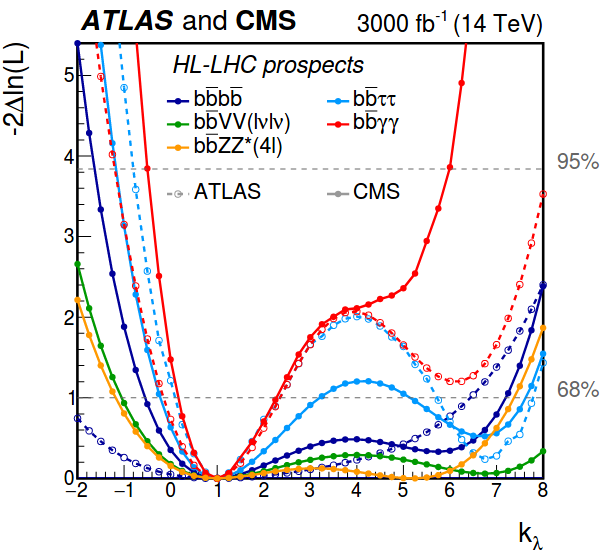
\includegraphics[width=0.46\textwidth]{Figures/HiggsPairProduction/projection2.png}}
\subfloat[]{\centering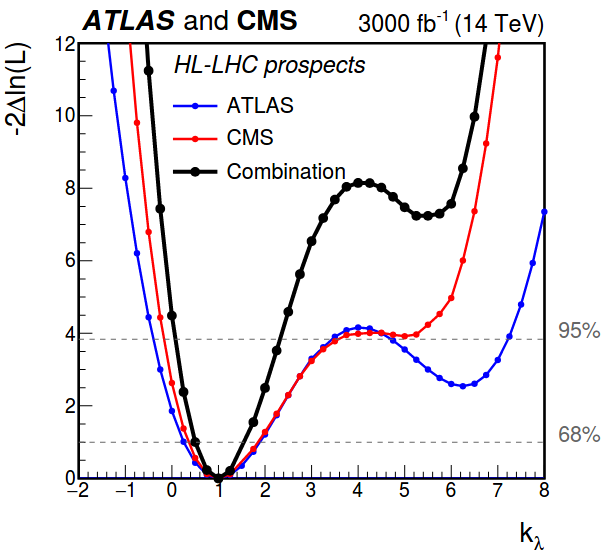
\includegraphics[width=0.46\textwidth]{Figures/HiggsPairProduction/projection1.png}}
\caption[Minimum negative-log-likelihood as a function of the $\kappa_{\lambda}$ modifier obtained by performing a fit to the expected background and SM signal]{Minimum negative-log-likelihood as a function of the $\kappa_{\lambda}$ modifier obtained by performing a fit to the expected background and SM signal~\cite{yellowreport}. A) Contours for different channels in the ATLAS and CMS projections, represented in dashed and solid lines, respectively. B) Combined results (black) from the CMS (red) and ATLAS (blue) projections.}
\label{fig:coklprojection}
\end{figure}

\chapter{Experimental Apparatus} 
\label{chapter:apparatus}
\section{The Large Hadron Collider}
European Center for Nuclear Research, or CERN, is the host of several experimental facilities. The CERN flagship experimental project is the Large Hadron Collider (LHC).  The CERN accelerator complex, located at the French-Swiss border, consists of a chain of machines that accelerate particles (e.g. protons and heavy ions) in various steps until the nominal energy for collisions is achieved. The accelerator complex is illustrated in Figure~\ref{fig:cernaccelerator}. 

\begin{figure}[ht]
\centering
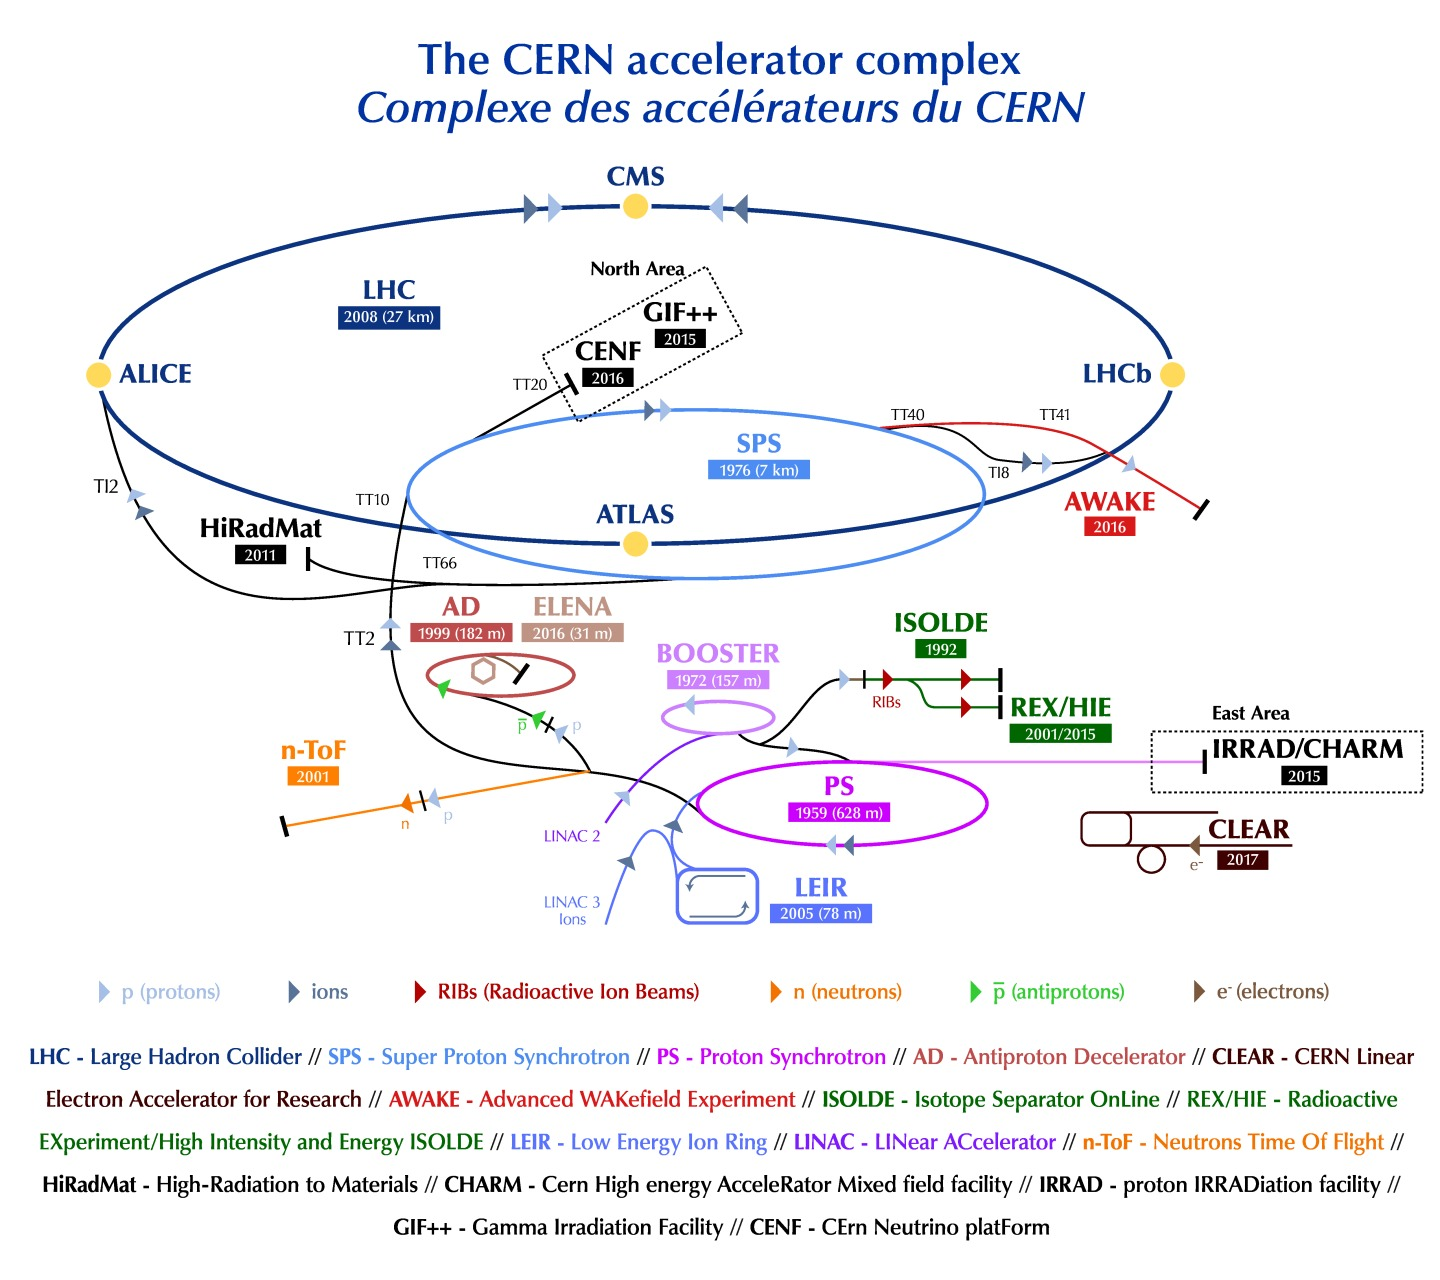
\includegraphics[width=0.9\textwidth]{Figures/Apparatus/cernmachines.jpg}
\caption[The CERN Accelerator Complex]{The CERN Accelerator Complex~\cite{Mobs:2197559}.}
\label{fig:cernaccelerator}
\end{figure}

The acceleration of protons starts by stripping the electrons on hydrogen atoms originally contained in a hydrogen bottle via a duoplasmatron proton source. Next, those protons are injected and accelerated successively by the LINAC-II, Booster, PS and SPS machines. The SPS output is a beam of protons organized in bunches with energy of 450 GeV, which is injected to the two LHC rings (one in clockwise and other in counter-clockwise direction). The two LHC beams are circulated in opposite directions and accelerated until they achieve an energy of around 6.5 TeV. Once the beams are stable, proton bunches with around $10^{11}$ protons each are collided. 

The LHC is a powerful tool that is capable to achieve high energy to probe the behavior of matter and its interactions. It is a circular superconducting accelerator and collider with 26.7 km of circumference, which is designed to produce pp collisions at up to 14 TeV of center-of-mass energy ($\sqrt{s}$) by colliding proton bunches every 25 nanoseconds in four interaction points (IPs) along the ring. There are experiments located at each of these points: ATLAS (A Toroidal LHC ApparatuS) and CMS (Compact Muon Solenoid) are general-purpose experiments that concentrate on measurements of SM processes and BSM physics searches at the TeV scale, the LHCb (LHC-beauty) experiment focuses on B-hadron physics, and ALICE (A Large Ion Collider Experiment) studies heavy-ion collisions phenomena (e.g. quark-gluon plasma). 

A key parameter to describe the collider operation is the instantaneous luminosity ($\mathcal{L}$), which depends on the beam properties as described in equation~\ref{eq:luminosity} and listed in Table~\ref{tab:lumiparameters}. The LHC operation was originally designed to achieve an instantaneous luminosity of around $\mathrm{10^{34}}$ $\mathrm{cm^{-2}~s^{-1}}$. High luminosities are important because they increase the production rate of interesting physics process, and thus our potential and sensitivity for physics discoveries. However, high luminosities imply the increase of the number of pp interactions per bunch crossing or pile-up (UP), which poses challenges to the experiments for reconstruction and radiation harness.
\begin{equation}
\label{eq:luminosity}
\mathcal{L}=\frac{ N_{b}^{2}~n_{b}~f~\gamma}{4\pi\epsilon\beta\sqrt{1 + (\frac{\theta_{c} \sigma_{z}} {2\sigma^{*}} )^{2} } }    
\end{equation}

The expected number of produced events of a particular process during the LHC collisions (without taking into account the detector acceptance) is predicted as $\mathrm{N=\sigma\cdot~L}$, where $\sigma$ is the theoretical production cross section ($\sigma$), and L is the integrated luminosity (L) defined as the integral of the instantaneous luminosity over the LHC operation time. The units of integrated luminosity are the inverse barn (b$^{-1})$, where $\mathrm{1~b^{-1} = 10^{24}~cm^{-2}}$.

\begin{table}[htb]
\centering
\caption[Parameters used in the calculation of the instantaneous luminosity at the Large Hadron Collider proton-proton collisions]{\label{tab:lumiparameters} Parameters used in the calculation of the instantaneous luminosity at the Large Hadron Collider proton-proton collisions~\cite{Bruning:782076}.}
\begin{tabularx}{\textwidth}{XX}
\hline
LHC design experimental parameters                      & Design or nominal values     \\
\hline
$f$, revolution frequency                               & 11.245 kHz        \\[0pt]
$n_{b}$, number of proton bunches per beam              & 2808              \\[0pt]
$N_{b}$, number of proton per bunch                     & 1.15 x $10^{11}$  \\[0pt]
$\beta$, optical beta function at the IP                & 55 cm             \\[0pt]
$\sigma_{Z}$,  RMS bunch length                         & 7.55 cm           \\[0pt]
$\sigma_{*}$,  transverse RMS beam size                 & 16.7 $\mu$m       \\[0pt]
$\gamma$, relativistic gamma factor                     & 7461              \\[0pt]
$\epsilon$, normalized transverse beam emittance        & 3.75 $\mu$m rad   \\[0pt]
$\theta_{c}$, crossing angle at the IP                  & 285  $\mu$rad     \\[0pt]
\hline
\end{tabularx}
\end{table}

The baseline plan of the LHC at past, present and future operations is presented in Figure~\ref{fig:lhcschedule}. The LHC particle beams were circulated for the first time in September 2008 but days later a failure of an electrical connection produced led to severe damage to the superconducting magnets, their connections and the vacuum pipe. After investigating the problem and over a year of repairing, the LHC beams were circulated back again in November 2009, and the first run of the LHC (Run-I) started at the beginning of 2010.
\begin{figure}[htp!]
\centering
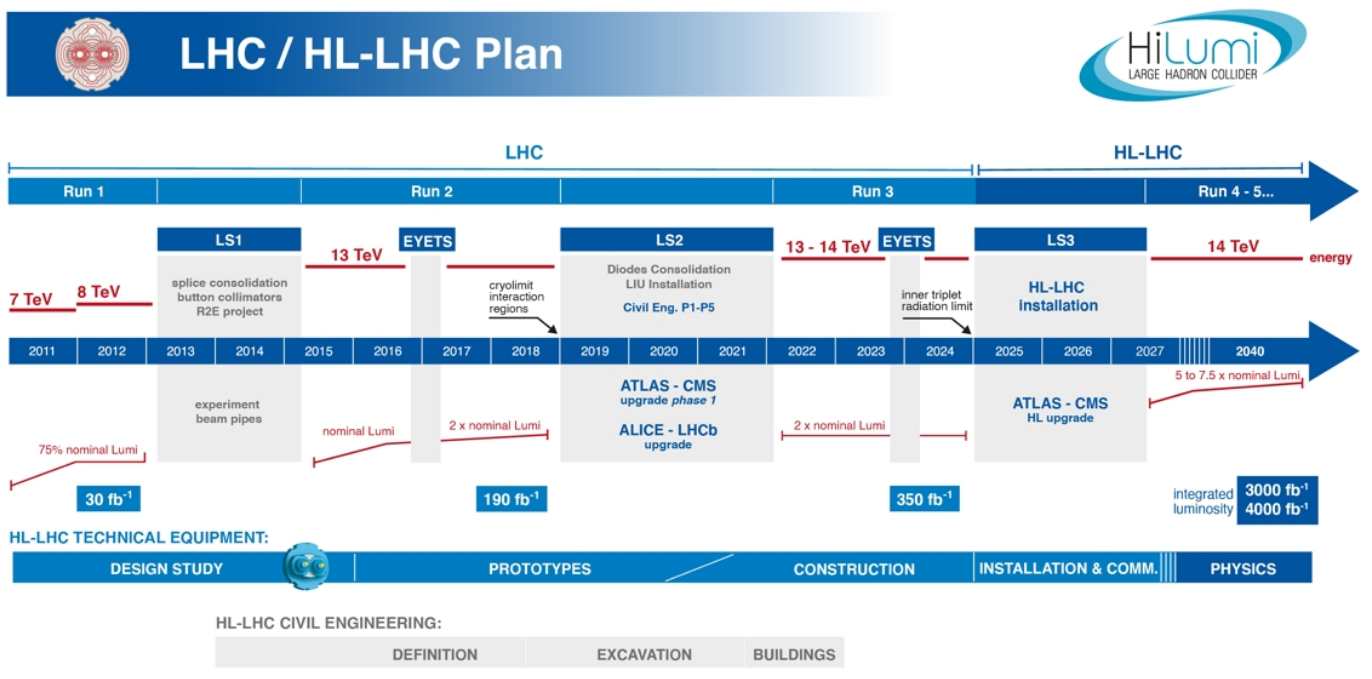
\includegraphics[width=1.0\textwidth]{Figures/Apparatus/lhcschedule.png}
\caption[The Large Hadron Hadron Collider schedule starting from Run-1 operations (2011) to the next decades and beyond.]{The Large Hadron Collider schedule starting from Run-1 operations (2011) to the next decades and beyond. In red, it is presented the expected proton-proton collision center-of-mass energy and the instantaneous luminosity.}
\label{fig:lhcschedule}
\end{figure}

%The LHC Run-1
In the LHC Run-1 (2010-2012), pp collision data was collected at $\sqrt{s}=$ 7 and 8 TeV with bunches crossing every 50 nanoseconds. The collected Run-1 dataset was analyzed for the discovery of the Higgs boson. Then, during the first long shutdown (LS1), 2013-2014, the LHC superconducting magnets were trained for the operation with 6.5 TeV proton beams, thus pp collisions at 13 TeV of center-of-mass energy. Moreover, detector upgrades took place. For instance, the CMS experiment performed the upgrade of its Level-1 trigger (hardware and architecture), in preparation for the Run-2 conditions.

%The LHC Run-2
The Run-2 operation of the LHC took place from 2015-2018, with 13 TeV pp collisions. The LHC reached a record instantaneous luminosity of $\mathrm{2.1~x~10^{34}}$ $\mathrm{cm^{-2}~s^{-1}}$, corresponding to an average of $55$ PU interactions. In CMS, the measured Run-2 average of PU interactions was around 34 as presented in Figure~\ref{fig:cmspileuprun2} A). The total integrated luminosity delivered by the LHC during the Run-2 operations was around 164 $\mathrm{fb^{-1}}$, as presented versus time in Figure~\ref{fig:cmspileuprun2} B). 

\begin{figure}[htp!]
\centering
\captionsetup[subfigure]{justification=centering}
\subfloat[]{\centering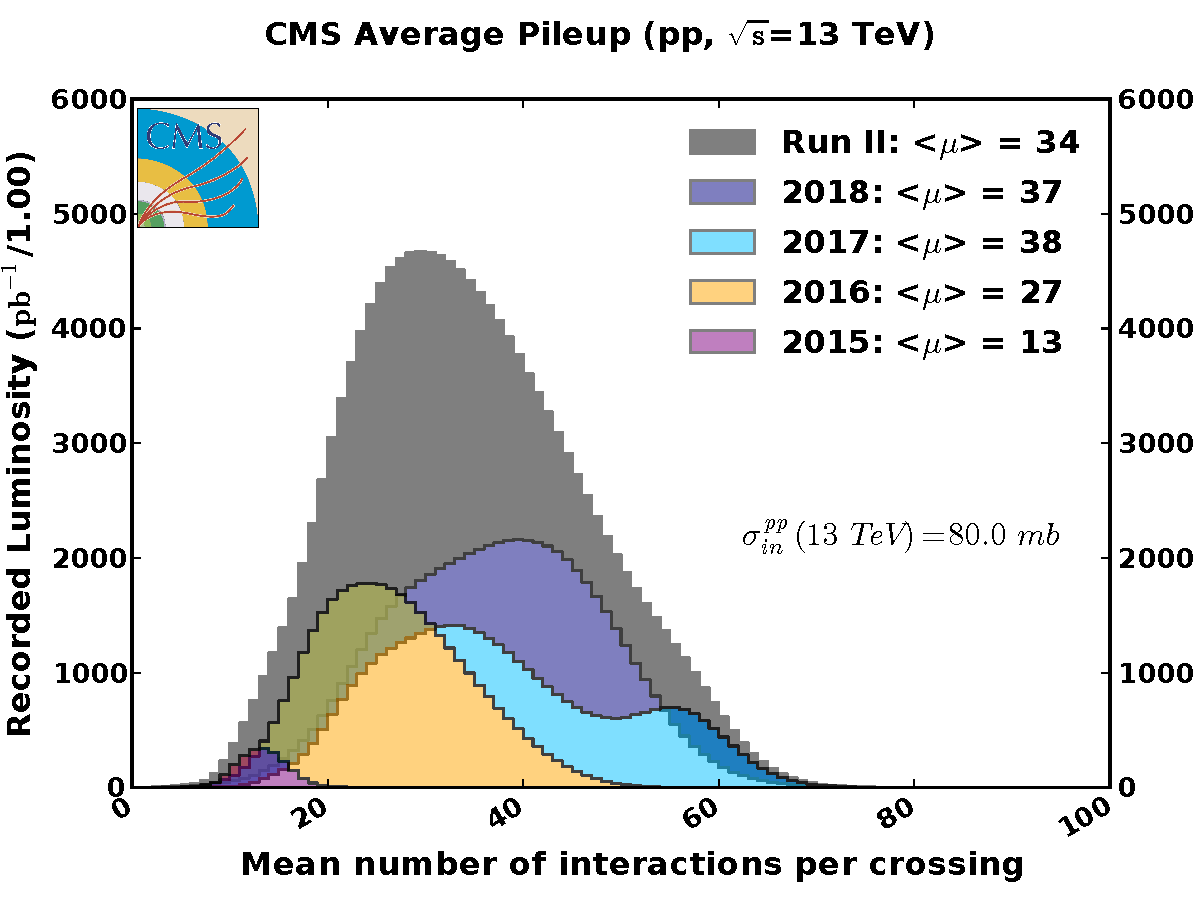
\includegraphics[width=0.45\textwidth]{Figures/Apparatus/pileup_allYears_run2.pdf}}
\subfloat[]{\centering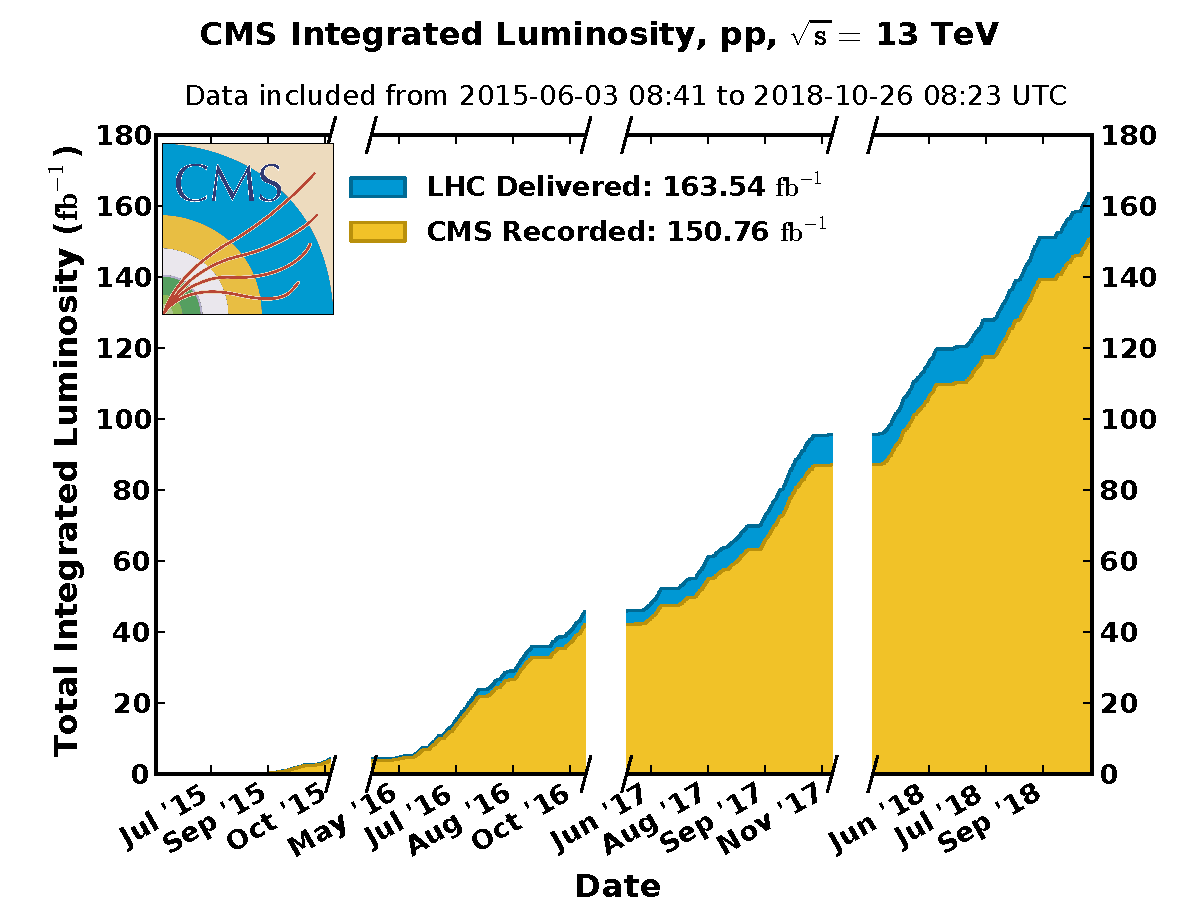
\includegraphics[width=0.45\textwidth]{Figures/Apparatus/int_lumi_allcumulative_pp_run2_cutout.pdf}}
\caption[CMS operation conditions in proton-proton collisions during the LHC Run-2 data-taking]{CMS operation conditions in proton-proton collisions during the LHC Run-2 data-taking. A) Distribution of pile-up average versus recorded luminosity, B) Total integrated luminosity versus time.}
\label{fig:cmspileuprun2}
\end{figure}

%Run-3 and the HL-LHC
At the time of writing this dissertation, the LHC is going under the second long-shutdown (LS2), 2019--2021, in preparation for the Run-3 operations. Due to the current Covid-19 pandemic, the LHC schedule has been delayed. Run-3 is expected to start at the beginning of 2022, and to last until 2024 or 2025. Then, after the third long shutdown (LS3) of 2--3 years, the LHC will operate at its ultimate high luminosity configuration, the HL-LHC. 

The HL-LHC operation period, expected to last for about a decade, is known as the LHC Phase-2. Phase-1 is the current operation until the end of Run-3. The HL-LHC accelerator is expected to produce 14 TeV pp collisions and to reach an instantaneous luminosity of 5--7.5 $\mathrm{x~10^{34}}$ $\mathrm{cm^{-2}~s^{-1}}$, corresponding to 200--300 average PU interactions. The expected dataset corresponds to 3000-4000 $\mathrm{fb^{-1}}$ of integrated luminosity (roughly 20-27 times more data than the one used in this dissertation). Major consolidation and upgrades of the LHC accelerator are ongoing in preparation for the HL-LHC era. The LHC experiments will undergo an important upgrade program to successfully operate in the challenging collision conditions (more in Section~\ref{subsec:cmsupgrades}).

\section{The CMS Experiment}
\subsection{Description}
The Compact Muon Solenoid (CMS) experiment is a general-purpose experimental apparatus located 100 meters underground within a cavern at the LHC Point 5 (P5) in Cessy, France~\cite{CMS:2008xjf}. The CMS detector surrounds the LHC IP with dedicated particle detector layers (or subsystems) to reconstruct the collisions products (electron, muons, photons, charged and neutral hadrons) and study the underlying physics phenomena. This detector has a cylindrical symmetry and is uniquely characterized by a high magnetic field superconducting solenoid. More details on the detector layers are presented by the next subsection.

\begin{figure}[htp!]
\centering
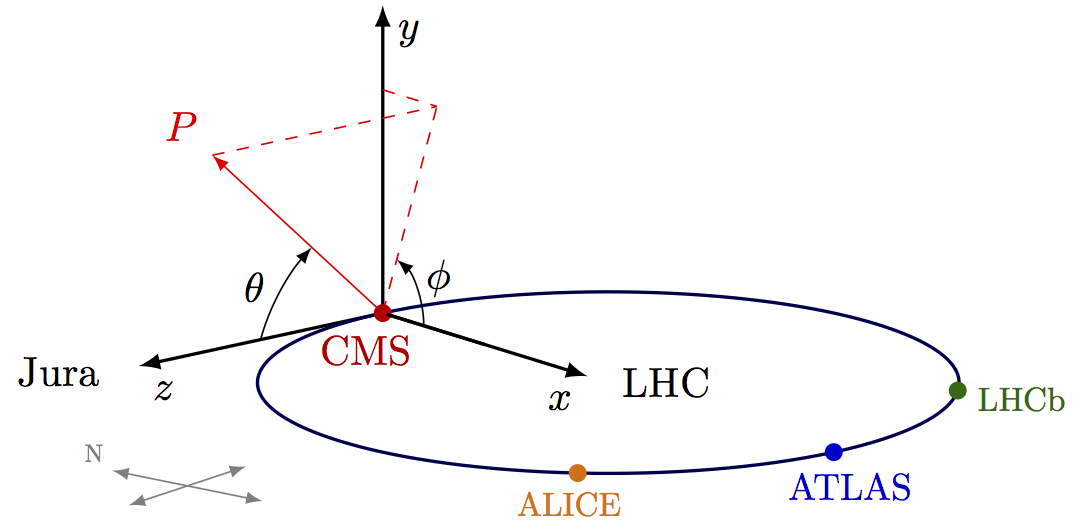
\includegraphics[width=0.95\textwidth]{Figures/Apparatus/cms_coordinate_system.png}
\caption[The CMS conventional coordinate system]{The CMS conventional coordinate system.}
\label{fig:coordinates}
\end{figure}

The conventional coordinate system used by CMS is illustrated in Figure~\ref{fig:coordinates}. The origin is fixed at the interaction point inside the detector. The X-axis points towards the center of the LHC, the Y-axis is perpendicular to the plane defined by the LHC ring, and the Z-axis is parallel to the beam line following the anticlockwise direction. The azimuthal angle $\phi$ is measured with respect to the X-axis over the X-Y plane. The polar angle $\theta$ is defined with respect to the Z-axis over the Y-Z plane.  The
$\theta$ angle is converted to the variable pseudorapidity $\eta$ by the relation $\eta=-\ln{[\tan{(\frac{\theta}{2}) }]}$. The angular distance between two points is measured in units of $\mathrm{\Delta R=\sqrt{ (\Delta\phi)^{2} + (\Delta\eta)^{2} }}$. The transverse component of vectorial properties such as the momentum are defined as the projection of the vector in the X-Y plane (e.g. transverse momentum $\mathrm{p_{T}}$). 

\subsection{Detector Layers}
At the LHC design luminosity, an average of 20 pile-up interactions are expected to occur simultaneously at the interaction point every 25 nanoseconds. Consequently, detectors with large number of channels and good timing resolution are needed to reconstruct and identify the products of the interaction under study with respect to the other interactions in the same bunch crossing. Moreover, the high-particle multiplicity environment ($\sim$1000 charged particles per bunch crossing) produce high radiation levels which can cause detector damage and thus, radiation-hard detectors/electronics are needed.

The CMS detector was designed to conduct a successful physics program involving diverse final states under the aforementioned data-taking constraints by satisfying the following detector requirements~\cite{CMS:2008xjf}:
\begin{itemize}
    \item Muon identification with good reconstructed momentum resolution ($<10\%$ at P$\sim$1 TeV)
    \item High momentum resolution and reconstruction efficiency of charged-particles
    \item Efficient triggering of $\tau$ leptons and b-quark hadronic jets
    \item Good resolution and efficient leptons and photons energy and isolation measurements
    \item Good missing-transverse energy measurement and dijet-mass through a hermetic, granular and angular coverage 
\end{itemize}

\begin{figure}[ht!]
\centering
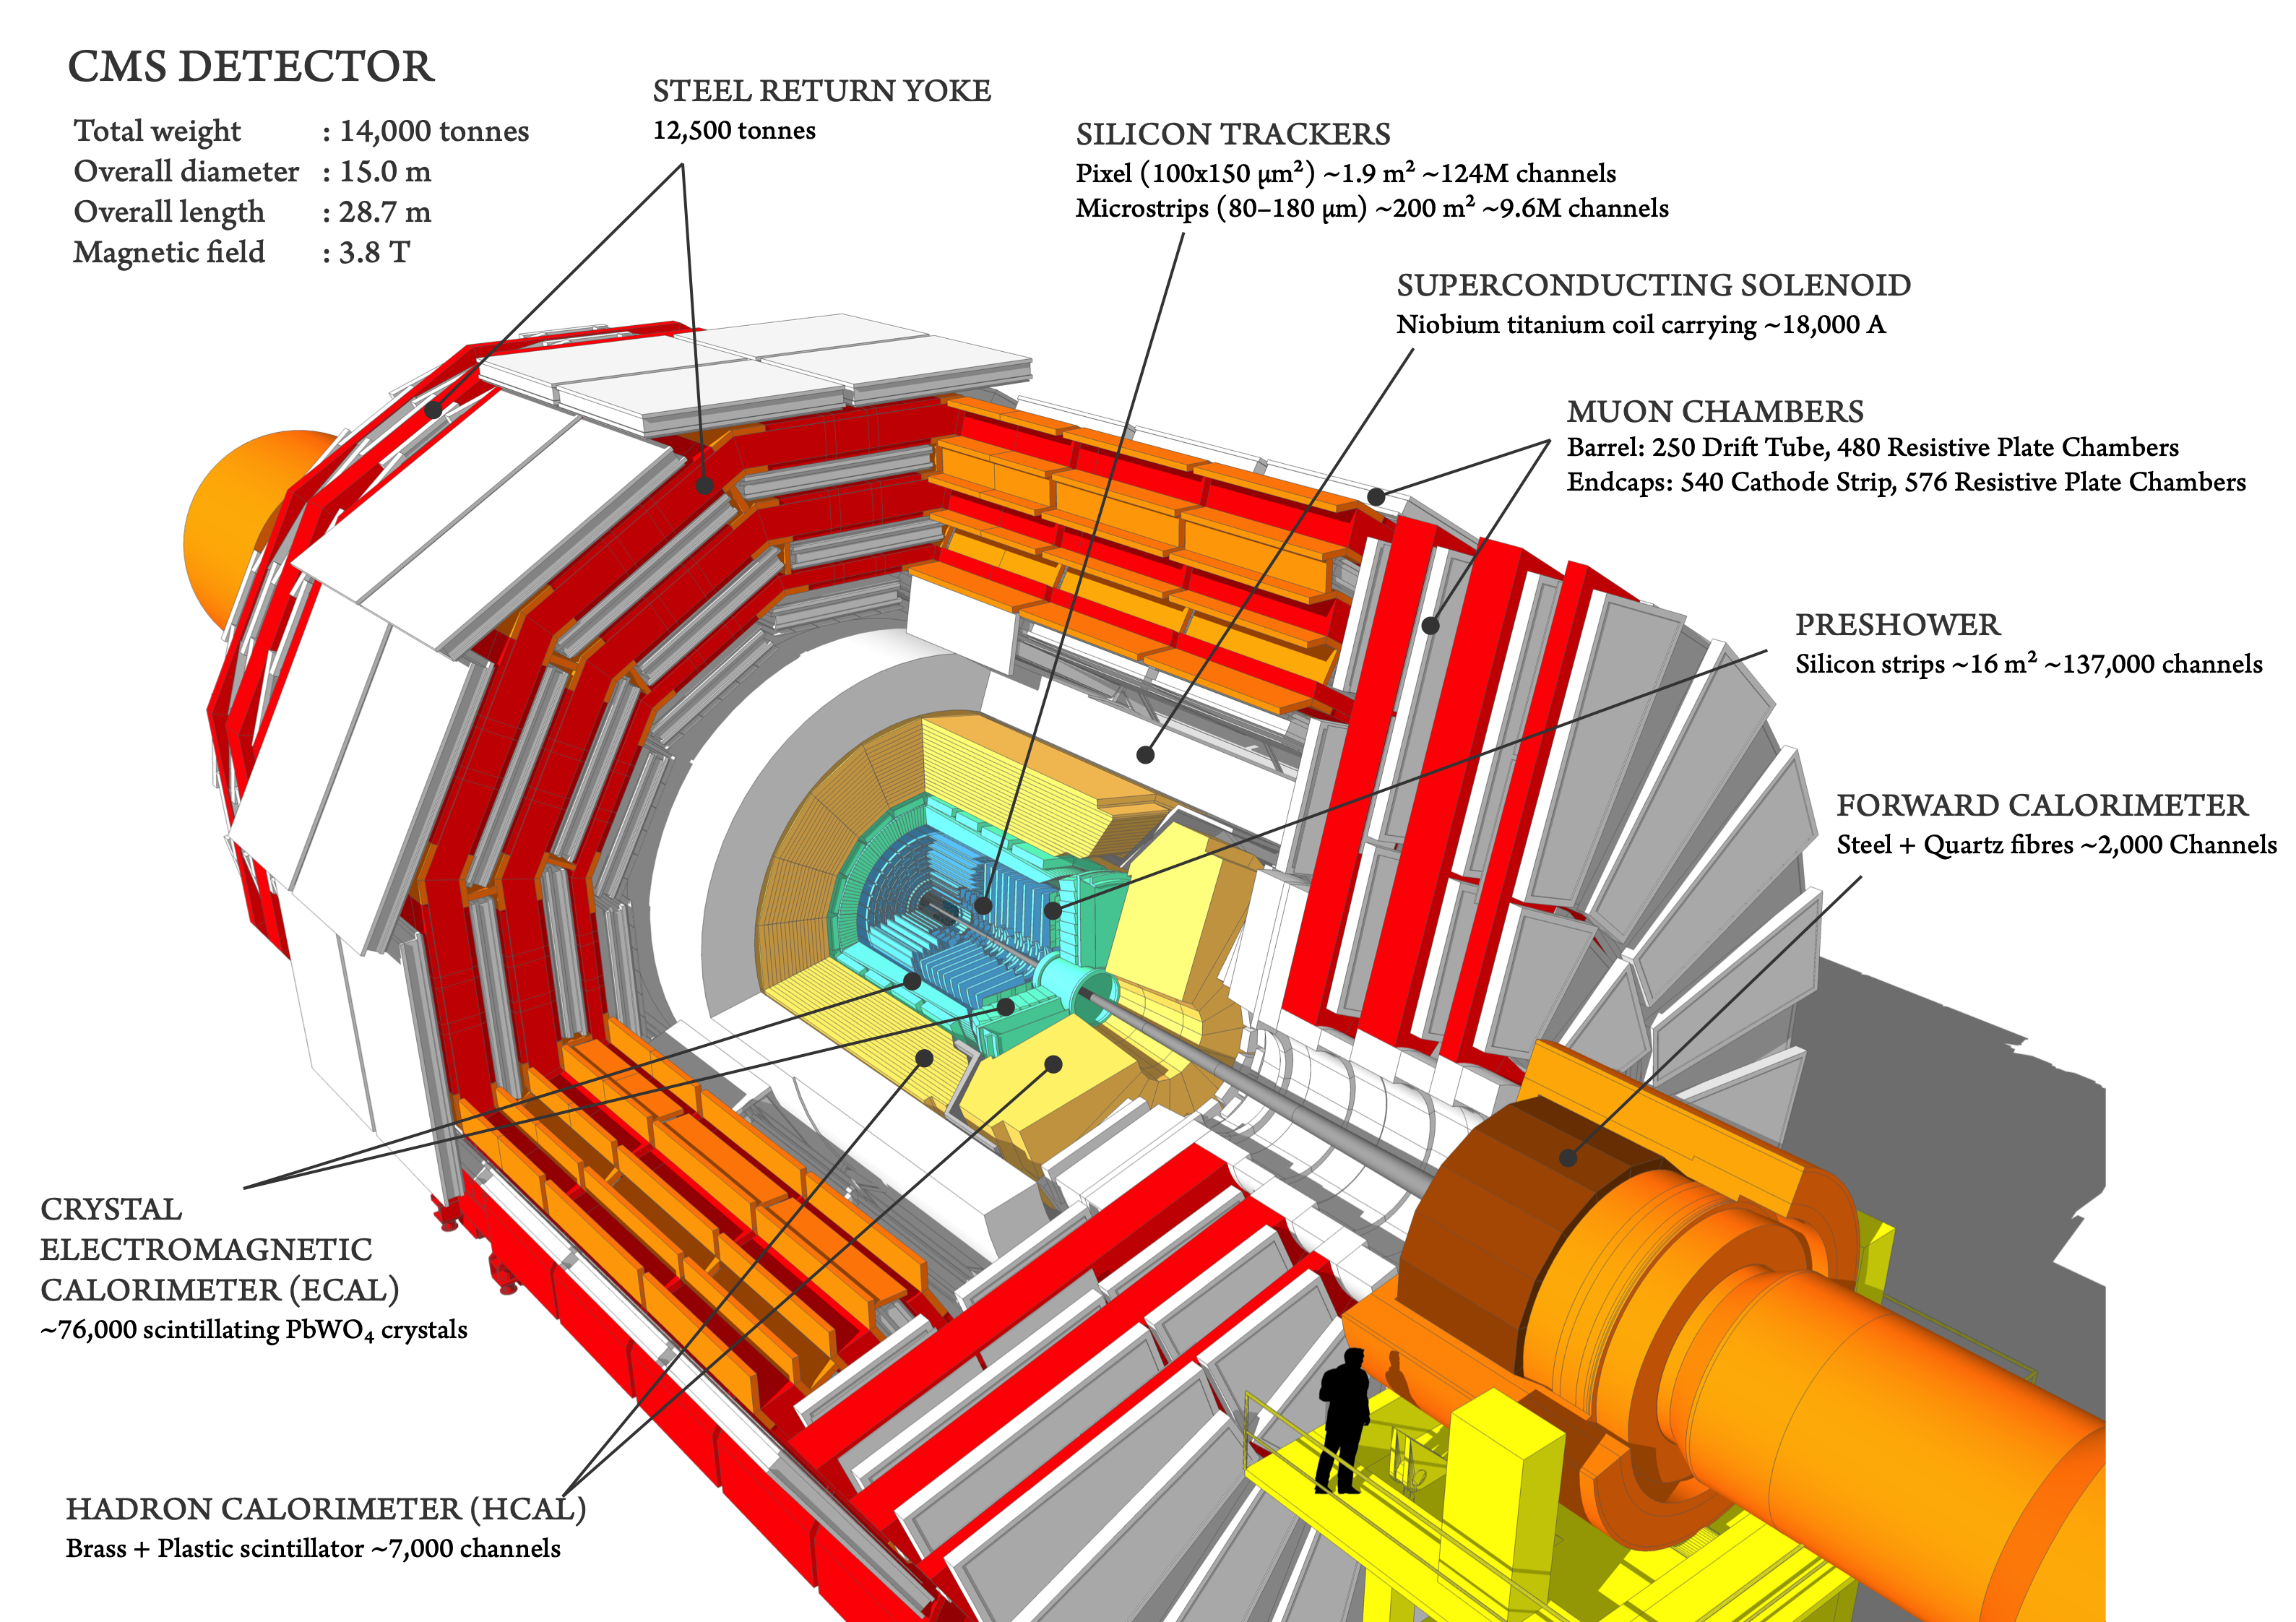
\includegraphics[width=1.0\textwidth]{Figures/Apparatus/cmsdetector.png}
\caption[Three-dimensional view of the subdetectors of the CMS experiment]{Three-dimensional view of the subdetectors of the CMS experiment.}
\label{fig:cmsdetector}
\end{figure}

The CMS detector layout and dimensions are presented in Figure~\ref{fig:cmsdetector}. A tracker, an electromagnetic and a hadron calorimeter are contained within the superconducting solenoid volume. The first detector layer is a full silicon-based inner tracking system composed of pixels and strip trackers, which information is processed to detect the interaction of charged particles and measure their trajectory and momentum. The energy of electromagnetic particles (photon and electrons) is measured from their energy deposits in a hermetic and homogeneous electromagnetic calorimeter layer made of lead tungstate (PbWO$_{4}$) crystals. Then, a hadronic calorimeter layer with a wide and hermetic coverage measures the energy of deposits from charged and neutral hadrons (e.g. pions). Then, the solenoid is surrounded by the muon system, which embedded in a steel flux-return yoke~\cite{CMS:2008xjf}.

\subsubsection{Inner tracking systems}
%motivation, purpose and capacity
The purpose of the inner tracking system is to provide an efficient and precise measurement of the trajectories of charged particles ($|
\eta|<2.5$), and to reconstruct the points of interactions of protons, referred to as vertices. This system has a primary importance to reconstruct the points of decay of B hadrons away from the beam line, or secondary vertices, which provide the main input to the jet flavor identification. Furthermore, it brings information for high-level triggers. The detector design has a high granularity, fast response, radiation hardness and as minimum material as possible (to reduce the impact on the momentum resolution from multiple scattering) to operate successfully under high collision rates, high particle flux and radiation levels. 

\begin{figure}[ht!]
\centering
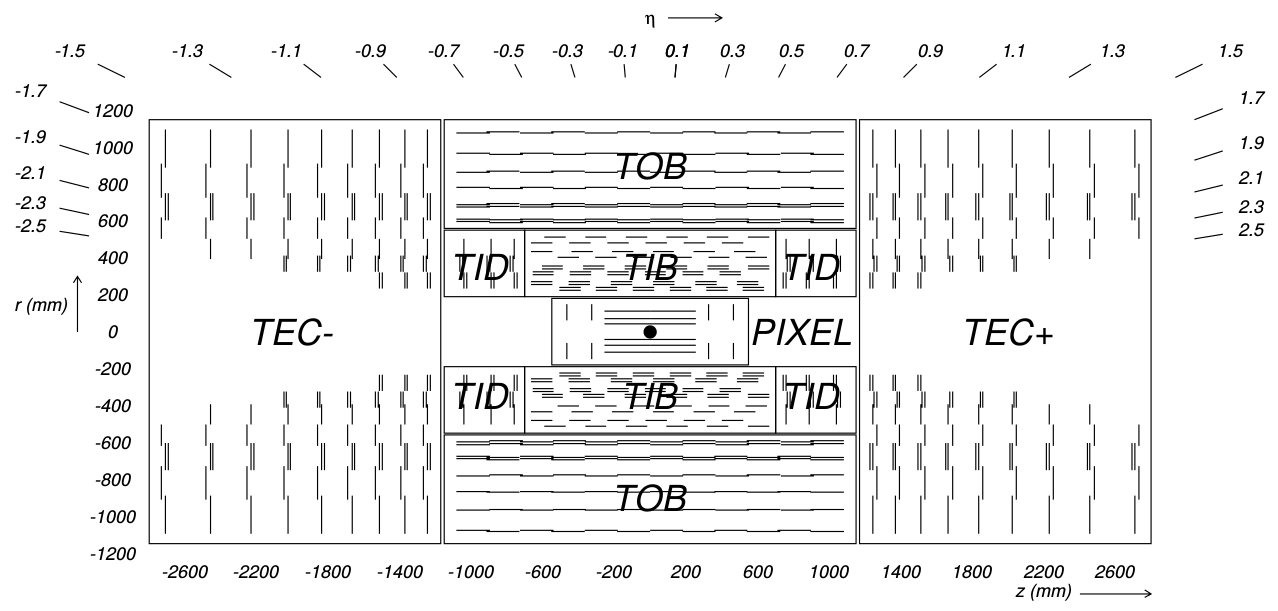
\includegraphics[width=0.9\textwidth]{Figures/Apparatus/cmstrackingsystem.png}
\caption[Layout of the CMS tracking system in the longitudinal direction]{Layout of the CMS tracking system in the longitudinal direction~\cite{CMS:2008xjf}. Note: This layout illustrates the Pixel detector before its upgrade.}
\label{fig:cmstrackingsystem}
\end{figure}
%layout
The layout of tracking system modules is illustrated in Figure~\ref{fig:cmstrackingsystem}. The Pixel tracking detector is the innermost part of the tracking system and thus the closest to the IP. The previous Pixel detector, used until 2016 data-taking, comprised of pixel detector modules organized in three cylindrical layers (BPIX) and two forward/backward disks (FPIX), covering an area of about 1 m$^{2}$ and 66 million pixels with hit resolution between 10-20 $\mathrm{\mu m}$. In the outermost tracking system is the Tracker detector. It comprises detector strip sensors with a total of 9.3 million strips covering 198 m$^{2}$ of area. The strips are organized in three subsystems: Tracker Inner Barrel and Disks (TIB/TID), Tracker outer barrel (TOB), and Track Endcap (TEC). The Tracker covers a pseudorapidity region up to $|\eta|=2.5$~\cite{CMS:2008xjf}.

The new or (upgrade) pixel detector was installed during the 2016/2017 shutdown in preparation for the 2017 data-taking, to maintain and improve the tracking performance under high luminosity conditions (up to $\mathrm{2~x~10^{34}}$ $\mathrm{cm^{-2}~s^{-1}}$ and exceeding an average of 50 pile-up interactions). The new detector consists of four cylindrical layers and three disks~\cite{cmspixelupgrade}. A comparison between the original and new pixel detector organization is illustrated in Figure~\ref{fig:cmstrackingsystemphase1}.

\begin{figure}[ht!]
\centering
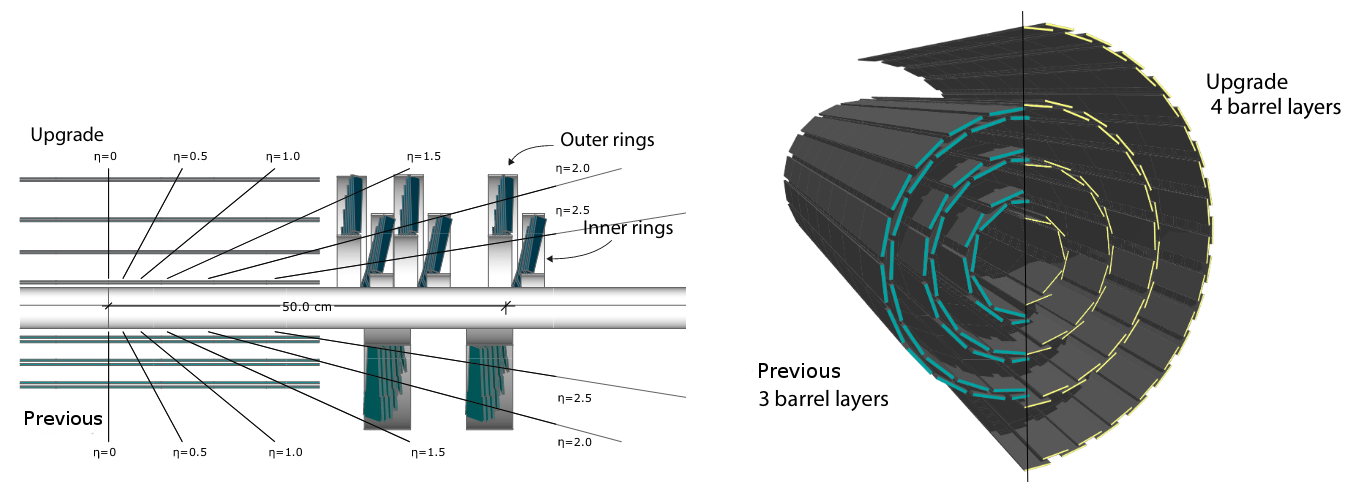
\includegraphics[width=0.9\textwidth]{Figures/Apparatus/cmstrackingsystemphase1.png}
\caption[The CMS pixel detector]{The CMS pixel detector~\cite{cmspixelupgrade}. Left: Half longitudinal section of the pixel detector layout previously (bottom) and after the upgrade (top). Right: Pixel barrel layers geometry previously (left) and after the upgrade (right).}
\label{fig:cmstrackingsystemphase1}
\end{figure}

\subsubsection{Electromagnetic calorimeter}
The electromagnetic calorimeter (ECAL) design was motivated in part by the goal of identifying two photons from the postulated Higgs boson. ECAL is a calorimeter based PbWO$_{4}$ crystals satisfying the requirements to operate under the LHC environment: hermetic, homogeneous, fast, fine granularity and radiation resistant. The radiation length ($X_{0}$) is the average length to reduce the energy of an incident electron by a factor of 1/e. The thickness of ECAL is larger than 25 $X_{0}$. The energy of the electromagnetic showers produced from incident photons/electrons is measured from associated scintillation light as is proportional to the incident particle energy. The scintillation light is collected by avalanche photodiodes (APDs) in the ECAL barrel region (EB, $|\eta|<1.48$), and vacuum phototriodes (VPTs) in the ECAL endcaps (EE, $1.48<|\eta|<3.0$). In addition, a preshower sampling calorimeter (ES) is located in front of the EE section covering $1.65<|\eta|<2.6$, as illustrated in Figure~\ref{fig:cmsecal} A), to help to initiate the electromagnetic showers from incoming photons/electrons, and to identify neutral pion decays into two photons.

The ECAL layout is presented in Figure~\ref{fig:cmsecal} B). A total of 61200 (7234) crystals of front-face cross section of around $\mathrm{22~x~22~mm^{2}}$ ($\mathrm{28.6~x~28.6 mm^{2}}$) and length of 230 (220) mm, are mounted on the EB (EE) region. The EB part is organized in 36 `supermodules', each covering half of the barrel region and divided in four modules. The crystals of the EE region are structured in 2 dees and grouped in units of 5x5 crystals denominated as `supercrystals'~\cite{CMS:2008xjf}.

\begin{figure}[htp!]
\centering
%\includegraphics[width=0.9\textwidth]{Figures/Apparatus/cmsecal.png}
\captionsetup[subfigure]{justification=centering}
\subfloat[]{\centering\includegraphics[width=0.43\textwidth]{Figures/Apparatus/cmsecalong.png}}
\subfloat[]{\centering\includegraphics[width=0.43\textwidth]{Figures/Apparatus/cmsecal.png}}
\caption[The CMS electrognetic calorimeter (ECAL)]{The CMS electromagnetic calorimeter (ECAL)~\cite{CMS:2008xjf,CMS:2006myw}. A) Longitudinal section of the geometrical configuration, B) Barrel and endcap configuration layout.}
\label{fig:cmsecal}
\end{figure}

The performance of the ECAL detector was studied through test beam measurements on a barrel supermodule using electron beams of energies between 20 and 250 GeV. The energy resolution ($\mathrm{ \frac{\sigma}{E} }$) can be parametrized as a function of the energy (E) using eq.~\ref{eq:energyresolution}, where S is the stochastic term, N is the noise and C is the constant term. The test beams measured the coefficients to be S=$2.8\%$, N=0.12 and C=$0.30\%$~\cite{CMS:2008xjf}. Then, the energy resolution of the was measured using ${Z\rightarrow e^{+}e^{-}}$ events in the 2010-2011 collision data. The measured resolution of the electrons with $\mathrm{E_{T}}\approx45$ GeV was around 2\% (2-5\%) in $|\eta|<0.8$ (elsewhere)~\cite{cmsecalrun1}. The excellent ECAL calibration and resolution performance were key for the 2012 Higgs boson discovery.
\begin{equation}
\mathrm{\left(\frac{\sigma}{E}\right)^{2} = \left(\frac{S}{\sqrt{E}}\right)^{2} + \left(\frac{N}{E}\right)^{2} + C^{2}}
\label{eq:energyresolution}
\end{equation}

\subsubsection{Hadronic calorimeter}
The hadronic calorimeter (HCAL) is an absorber/scintillator sampling calorimeter surrounding ECAL. It measures the energy of charged and neutral hadrons, which is crucial for the reconstruction of hadronic jets and the missing transverse energy from neutrinos (or exotic particles). Incident hadrons interact with the absorber via nuclear force and generate hadronic showers in the absorber and scintillator. Then, the associated scintillator light is collected by wavelenghth-shifting fibres (WLS) and channeled to photodetectors for readout. The interaction length ($\mathrm{\lambda_{I}}$) of a material is the average distance a hadron travels before an inelastic nuclear interaction. Depending on $\eta$, the HCAL thickness varies within 10-15 $\mathrm{\lambda_{I}}$, and thus a good containment of the hadronic shower~\cite{CMS:2008xjf,CMS:2006myw}. HCAL is divided by four subdetectors: Hadron barrel (HB, $|\eta|<1.4$), Hadron outer (HO), Hadron Endcap (HE, $1.3<|\eta|<3.0$) and Hadron forward (HF, $3.0<|\eta|<5.0$). The layout of the HCAL detector is presented in Figure~\ref{fig:cmshcal}.

\begin{figure}[ht!]
\centering
\includegraphics[width=0.8\textwidth]{Figures/Apparatus/cmshcal.png}
\caption[Longitudinal layout of the CMS hadronic calorimeter (HCAL)]{Longitudinal layout of the CMS hadronic calorimeter (HCAL)~\cite{CMS:2008xjf}.}
\label{fig:cmshcal}
\end{figure}

The HB and HE are brass/plastic scintillator tiles sampling calorimeters located inside the solenoid. In the HB and HE sections, there are a total of 2304 readout `towers' formed from the scintillator tiles with a  segmentation of $\mathrm{(\Delta\eta,\Delta\phi)=(0.087,0.087)}$ and $\mathrm{(\Delta\eta,\Delta\phi)=(0.17,0.17)}$, respectively. The HCAL photodetectors are multichannel hybrid photodiodes (HPDs). HO and HF subdetectors are located outside the solenoid. The HO subdetector provides additional layers of scintillator to sample the energy of hadron showers leaking from the rear of the calorimeters, improving the $\mathrm{E_{T}}$ resolution. The HF calorimeters, located at around 11 meters from the interaction point, consist of steel absorber and quartz-fiber layers. Signals come from the Cerenkov light emitted from the quartz fibers, which is collected by photomultipliers (PMTs). The HF materials were chosen in order to contain hadronic showers from energetic forward jets in the intense radiation levels in the forward region~\cite{CMS:2008xjf,CMS:2006myw}.

%Maybe here write about the HCAL+ECAL performance in jet energy or MET resolution
\subsubsection{Superconducting solenoid}
The CMS superconducting solenoid (or magnet) plays a key role in bending the trajectories of charged particles to perform a precise measurement of their transverse momentum using the tracking and muon systems.  An artistic illustration of the CMS magnet is presented in Figure~\ref{fig:cmsmagnet}. It is design to reach a 4 T magnetic field and 2.6 GJ of stored magnetic energy within a cylindrical region with 6 m of diameter and 12.5 m of length. The magnet `cold mass' consist of a 4-layer winding of a reinforced NbTi conductor within a cryostat operating at 1.2 K~\cite{CMS:2008xjf,CMS:2006myw}. 

\begin{figure}[htp!]
\centering
\includegraphics[width=0.8\textwidth]{Figures/Apparatus/cmsmagnet.png}
\caption[Three-dimensional artistic view of the CMS magnet]{Three-dimensional artistic view of the CMS magnet~\cite{CMS:2008xjf}.}
\label{fig:cmsmagnet}
\end{figure}

The magnetic flux is returned through an iron yoke, which comprises 5 wheels (-2,-1,0,1,2) in the barrel region, and two endcaps, as seen in Figure~\ref{fig:cmsdetector}. The iron yoke holds the detectors of the muon system, and it serves as hadron absorber.

\subsubsection{Muon system}
The precise measurement of muons is crucial in the CMS experiment because those particles are produced in many interesting signatures. One example is the Higgs boson decay into a Z boson pair with four muons in the final state ($\mathrm{H\rightarrow ZZ\rightarrow4\mu}$), which was the golden channel in the Higgs boson discovery due to the excellent mass resolution. The muon system is designed for muon identification, precise momentum and charge reconstruction, and triggering over the kinematic range of the LHC. In Figure~\ref{fig:cmsmuonsystem} is illustrated the layout of the CMS muon system and its three types gaseous chambers: Drift tubes (DTs)~\cite{cmsdtscosmicrays}, Cathode strip chambers (CSCs)~\cite{cmscscscosmicrays} and Resistive Plate Chambers(RPCs)~\cite{cmsrpcscosmicrays}. Depending on $\eta$, different detector types are mounted to achieve an efficient detector response in the full region of $|\eta|<2.4$~\cite{CMS:2008xjf,CMS:2006myw}. 

\begin{figure}[ht!]
\centering
\includegraphics[width=0.9\textwidth]{Figures/Apparatus/cmsmuonsystem.pdf}
\caption[One quadrant of the CMS muon system in the longitudinal direction]{One quadrant of the CMS muon system in the longitudinal direction. Drift tubes (DTs), Cathode strip chambers (CSCs) and Resistive Plate Chambers are presented in orange, green and blue color, respectively.}
\label{fig:cmsmuonsystem}
\end{figure}

In the barrel region, the neutron-induced background is small, the muon rate is low, and the magnetic field is approximately constant. Consequently, a total of 250 DT chambers are used in the $|\eta|<1.2$ region. They are organized in 4 stations (or radial layers) and embedded in the flux-return yoke wheels. In the endcap region, the muon rates and background levels are high, and the magnetic field is not uniform. Therefore, CSCs are used in the $0.9<|\eta|<2.4$ region due to their fast timing, fine segmentation and radiation hardness. A total of 468 CSCs are positioned in the two endcaps. RPCs are characterized by a fast response, good time resolution, but have lower space resolution than CSCs and DTs chambers. A set of RPCs is added in both barrel and endcap regions covering $|\eta|<1.6$, to identify the correct bunch crossing, increase muon hit redundancy to reduce background, and resolve ambiguities from multiple hits in the same chamber~\cite{CMS:2008xjf,CMS:2006myw}. 

\subsection{Event Reconstruction}

A global description of the collision event, where all stable particles are identified, can be achieved by the correlating and combining the detector information associated to their interaction with the different subdetectors (illustrated in Figure~\ref{fig:cmspfslice}). This type of approach is denominated as Particle-Flow (PF) reconstruction, and first was used by the ALEP experiment at the LEP $\mathrm{e^{+}e^{-}}$ collider~\cite{alephpf}. The CMS design properties (e.g. fine-granularity of the detectors) enable the use of the PF reconstruction. Since the first implementation of it for physics analysis in 2009 and triggering in 2010, all physics analyses use PF reconstruction. 

\begin{figure}[ht!]
\centering
\includegraphics[width=0.95\textwidth]{Figures/Apparatus/cmspfslice.png}
\caption[A transverse slice of the CMS detector representing the interaction of stable particles]{A transverse slice of the CMS detector representing the interaction of stable particles (electron, muon, photon, charged and neutral hadrons) with each of the subsystems.}
\label{fig:cmspfslice}
\end{figure}

The basic PF elements are tracks and calorimeter clusters. Then, they are used for PF identification and reconstruction to produce PF objects/candidates associated to muons, electrons, photons, charged and neutral hadrons. The PF candidates are used after for building more complex physics objects such as hadronic jets, tau leptons, and missing transverse momentum. The PF candidates are the objects used for physics analysis. In what follows it is summarized the CMS methods use to reconstruct all event objects in the context of the PF algorithm. More detailed information is found in Ref.~\cite{cmspfalgo}.

\subsubsection{Tracks and calorimeter clusters}
Experimentalists use track-finder algorithms to find a set of detector hits/stubs compatible with a charged particle track. Then, a fit is performed to obtain the track properties (origin, momentum, direction, etc.). The trajectories of charged particles crossing the CMS inner tracking system (inner track) are reconstructed from hits using an iterative tracking method. In this approach, a combinatorial track finder based on Kalman Filtering (KL) is applied in ten successive iterations. Each iteration has a dedicated seeding and type of track target. The hits associated with built tracks are masked in the next iteration. The reconstruction efficiency surpasses the one from single iteration methods and keeps misreconstruction rates at similar levels~\cite{cmspfalgo}.

The muon system tracking is performed with high efficiency over the different regions of the detector, and independent of the tracker-based or PF reconstruction. There are three possible types of muons:
\begin{itemize}
    \item Standalone muon: The muon track is reconstructed from the information of the CSC, DT and RPC hits using a pattern recognition algorithm for hit selection and a fit method for getting the track properties
    \item Tracker muon: It is an inner track with $\mathrm{p_{T}>0.5~GeV}$ and $\mathrm{p>2.5~GeV}$, which matches with at least one muon hit when extrapolated to the muon system.
    \item Global muon: Standalone muon tracks are matched to inner tracks. Then, for each match that is found, all associated hits are used to fit a global muon track. 
\end{itemize}
A dedicated clustering algorithm is used to generate clusters from the energy deposits in the calorimeters. The clustering method is performed independently by ECAL, HCAL and preshower detectors. In essence, the clustering is as follows. First, cluster seeds are found based on cells passing a seed threshold and larger energy with respect to their neighbors. These neighbors can be the four cells sharing a side (HCAL) or eight cells sharing corners and sides (ECAL and preshower). Then, topological clusters are formed by adding to the seed cluster more cells with at least a common corner and energy twice the noise level. Lastly, an algorithm based on a Gaussian-mixture model reconstruct the clusters with position and energy from the topological cluster. This clustering method applied at HF because the electromagnetic or hadronic component of a cell can be separated into HF EM cluster and HF HAD cluster, respectively~\cite{cmspfalgo}. 

\subsubsection{Particle-flow identification and reconstruction}

In the PF algorithm, the process starts with an algorithm that links PF elements based on the nearest neighbors obtained with a k-dimensional tree across the $(\eta,\phi)$ plane. The link conditions depend on the PF elements involved. The output is called PF blocks, consisting of PF elements with a direct or indirect (via common elements) links. Then, the next step is to identify and reconstruct the particles in each PF block~\cite{cmspfalgo}. 

%Muons
Muons are the first identified particles in the PF block. The muon identification is performed based on the global-muon and tracker-muon properties. The identification minimizes the muon misidentification of charged hadrons. Isolated global muons are identified by taking into account the characteristics of the surrounding tracks and calorimeter deposits within $\mathrm{\Delta R}=0.3$. Non-isolated global muons are identified using tight-muon requirements, at least three muon station segments, and calorimeter deposits compatible with muons, reducing the muon misidentification of high-$\mathrm{p_{T}}$ hadrons. The momentum of the muon is the one from the inner track if $\mathrm{p_{T}}<200$ GeV. Otherwise, the $\mathrm{p_{T}}$ associated to the track fit minimizing the $\chi^{2}$ is chosen. Once the PF muon candidates are found, their PF elements are masked against further processing~\cite{cmspfalgo}.

%Electrons and isolated photons
Electrons are the second objects that are studied in the PF block. When electrons propagate in the inner tracker materials, they often emit bremsstrahlung photons before reaching ECAL. These photons can also produce $e^{+}e^{-}$ pairs, they can emit more photons, and so on. The PF algorithm combines the track and calorimeter information for identification and reconstruction, collecting the energy of soft and energetic radiated photons. Isolated photon identification and reconstruction are performed in the same step~\cite{cmspfalgo}

The ECAL-based seeding of electrons uses the information of ECAL clusters ($\mathrm{E_{T}>4~GeV}$), to infer the position of the hits associated to well isolated and energetic electrons. The energy is determined by grouping clusters into superclusters within a small $\eta$ window and extended $\phi$ window, compatible with the electron magnetic bending. The performance of this method relies on gathering all emitted photons, and thus, this approach is not efficient for non-isolated electrons in jets or soft-$\mathrm{p_{T}}$ electrons. Therefore, a tracker-based seeding for electrons is performed to complement the ECAL-based seeding. First, all inner tracks passing a dedicated preselection ($\mathrm{p_{T}>2~GeV}$, number of hits and the fit $\chi^{2}$ cuts) are fitted again with a Gaussian-sum filter (GSF). These GSF tracks are more compatible with the electron hypothesis as account for the large energy losses along the trajectory~\cite{cmspfalgo}. 

In the PF block, the electron candidate is seeded from a GSF track linked to an ECAL cluster with no more than three additional track links, whereas a photon candidate is seeded from a ECAL cluster with $\mathrm{E_{T}>10~GeV}$ and without GSF track link. All ECAL clusters linked to the superclusters or the GSF track are associated to the candidates. Tracks linked to these ECAL clusters are associated to the candidate if the track momentum and the energy of the linked HCAL cluster is compatible with the electron hypothesis. The photon energy is obtained from the total energy of the associated ECAL clusters, which is corrected as a function of energy and $\eta$, to account for any misses during the association process. The photon direction is the one of the supercluster. The electron energy is assigned from corrected ECAL energy and GSF track momentum information, while the electron direction is taken from the GSF track~\cite{cmspfalgo}.  

Non-isolated and isolated PF electron candidates must satisfy a threshold on a multivariate score based on dedicated BDTs trained with up to 14 variables. If photons are isolated from tracks and calorimeter clusters, and the HCAL - ECAL ratio is compatible with the electron hypothesis, then they are classified as PF photons. All tracks and ECAL or preshower clusters associated to the PF electrons and isolated photons are excluded from further processing~\cite{cmspfalgo}.

%Hadrons and non-isolated photons
The last candidates classified in the PF block are charged hadrons (e.g. $\pi^{\pm}$ and protons), neutral hadrons (e.g. neutrons), and non-isolated and soft photons (e.g. $\pi^{0}\rightarrow\gamma\gamma$), typically produced in hadronic processes (e.g. jets). Within the tracker acceptance ($|\eta|<2.4$), all isolated ECAL (HCAL) clusters without a track link are identified as photons (neutral hadrons), while charged hadron candidates are identified from the HCAL clusters with track link. However, beyond the tracker acceptance, there is no distinction between charged and neutral hadrons. In this case, ECAL clusters with a HCAL-link are assumed to be hadron candidates, otherwise, if there is no such link, they are classified as photon candidates. Then, photon and hadron energies are calibrated from their raw calorimeter energies. HF EM and HF HAD clusters are classified as HF photons and HF hadrons, respectively~\cite{cmspfalgo}.

\subsubsection{Jet reconstruction and flavor identification}

The quark or gluon hadronization generates a collimated shower of particles, which experimental signature is known as hadronic jet or jet. The jet is reconstructed using physical objects such as calorimeter towers or clusters (Calo jets), PF candidates (PF jets) or simulated/generated particles (Gen/Ref jets). A jet clustering algorithm determines which objects are included in the jet. A good jet algorithm is infrared and collinear safe, i.e. the set of jets should be unchanged by soft gluon emission and collinear splitting. Typically, the jet algorithms iteratively find two objects in the event which are closest based on a defined metric and combines them. Then, the jet 4-vector is obtained from the sum of all constituent particle 4-vectors. 

In the CMS experiment, the most used jet clustering algorithm is the $\mathrm{anti-k_{T}}$~\cite{Cacciari:2008gp,Cacciari:2011ma}. A radius parameter of R = 0.4 (0.8) is used to reconstruct small-cone jets (large-cone) jets, known as AK4 (AK8) jets. The AK4 PF (Calo) jets are typically used requiring $\mathrm{p_{T}>15 (20)~GeV}$, otherwise they are considered unreliable. The reconstruction of a di-jet simulated event is illustrated in Figure~\ref{fig:recojets}, where it is observed the good performance of PF jets with respect to Calo jets. Note that tracks and clusters produced from PU interactions can impact the performance of the jet reconstruction. This is mitigated with the charged-hadron subtraction (CHS) method, which excludes any charged particles pointing towards reconstructed PU vertices from the jet clustering and assigns the jet 4-momenta correction from the impact of neutral PU particles~\cite{cmspfalgo}.

\begin{figure}[ht!]
\centering
\includegraphics[width=0.6\textwidth]{Figures/Apparatus/dijetreco.png}
\caption[Reconstruction of a di-jet in a simulated event without pile-up]{Reconstruction of a di-jet in a simulated event without pile-up. The jet reconstruction is performed using calorimeter (Calo) jets, PF jets, and generated (Ref) jets. No jet corrections are applied~\cite{cmspfalgo}.}
\label{fig:recojets}
\end{figure}

%JET CORRECTIONS
The reconstructed jets are calibrated to correct their jet energy scale (JES). Jet energy corrections (JEC) as function of $\mathrm{p_{T}}$ and $\eta$ are derived from several dedicated measurements performed using data and simulated events. They address sequentially the impact of pile-up, uniformity of the detector response, and residual data-simulation differences. Furthermore, the jet energy resolution is measured using di-jet and photon+jet events to derive correction for differences between data and simulation. The energy resolution (JER) of central jets is around 15--20\%, 10\% and 5\% for a jet $\mathrm{p_{T} = 30}$ GeV, 100 GeV and 1 TeV, respectively~\cite{CMS:2016lmd}. 
%Jet ID and PU ID
There are jet algorithms developed to reject non-physical jets. Noise jets, originating from calorimeter noise or misreconstruction of electron/muon candidates, are rejected using the PF jet identification criteria, known as PF Jet ID. Moreover, the identification of jets formed from PU particles (PU jets) is performed via the PU ID technique, which permits rejecting those type of jets using a BDT score~\cite{CMS:2017wyc}. 

%Jet b-tagging
Several SM and BSM physics processes have a final state containing heavy-flavor hadronic jets, i.e. jets from b quark (b jets) and c quark hadronization (c jets). Therefore, it is crucial to develop dedicated algorithms for jet flavor assignment or `tagging', to efficiently reconstruct those processes, and reject background associated to light-flavor jets from light-quark and gluon hadronization. Heavy flavor tagging algorithms exploit the physical properties and correlations of the reconstructed jet and its constituents. For instance, one distinctive heavy-flavor jet characteristic is the production of a displaced secondary vertex. As b (c) hadrons (produced during b quark hadronization) have a lifetime of around 1.5 (1) ps, consequently, they have a flight distance a few mm - cm with respect to the primary vertex before decaying into other particles (e.g. charged lepton). The experimental signature is a displaced secondary vertex formed from displaced tracks within the jet. This is illustrated in Figure~\ref{fig:bjet}.

\begin{figure}[htp!]
\centering
\includegraphics[width=0.5\textwidth]{Figures/Apparatus/bjet.png}
\caption[Heavy-flavour (b quark or c quark) jet kinematic properties]{Heavy-flavor (b quark or c quark) jet kinematic properties~\cite{cmsbtagging13tev}.}
\label{fig:bjet}
\end{figure}

CMS analysts have used heavy-flavor tagging algorithm in data analysis since Run-1~\cite{cmsbtagging8tev}. For Run-2 data analysis, new and more sophisticated algorithms based on deep learning methods have been developed~\cite{cmsbtagging13tev,cmsbtagging13tev2}. The DeepJet algorithm for AK4 jets is the best to date in CMS~\cite{cmsdeepjet}. It is based on a sophisticated deep neural network with a total of 650 inputs from four categories: PF charged candidates, PF neutral candidates, secondary vertex features, and global event variables. The DeepJet multi-output layer is integrated into a multiclassifier which performs b-tagging, c-tagging, and quark/gluon tagging. The performance of this algorithm surpasses significantly the previous algorithms~\cite{cmsbtag1} as illustrated in Figure~\ref{fig:deepjet}. This dissertation uses the DeepJet for b-tagging. 

\begin{figure}[ht!]
\centering
\captionsetup[subfigure]{justification=centering}
\includegraphics[width=1.0\textwidth]{Figures/Apparatus/deepjet.png}
\caption[Performance of the DeepJet algorithm with respect to the DeepCSV algorithm]{Performance of the DeepJet algorithm with respect to the DeepCSV algorithm in simulated hadronic top quark pair ($\mathrm{t\overline{t}}$) events~\cite{cmsdeepjet}. Mis-id rates vs b-tagging efficiency for jets with $\mathrm{p_{T} > 30 GeV}$.}
\label{fig:deepjet}
\end{figure}

\subsubsection{Tau reconstruction}
The $\tau$ leptons are the most massive charged leptons in Nature (m$_{\tau}\sim1.77$ GeV). The $\tau$-leptonic decays (e.g. $\tau^{-}\rightarrow e^{-} \overline{\nu_{e}}\nu_{\tau}$ ) have a 35.2\% branching fraction. Moreover, $\tau$ leptons are massive enough to have almost all remaining decays involving hadrons (charged hadrons and neutral pions), known as $\tau$-hadronic decays ($\tau_{h}$).

As the two neutrinos escape detection, the $\tau_{l}$ decays are identified through the involved electron or muon candidate. On the other hand, $\tau_{h}$ decays are identified and reconstructed using the Hadron-Plus-Strip (HPS) algorithm since Run-1 data. This method reconstructs the $\tau_{h}$ decay by combining the information from charged hadrons and $\pi^{0}$ candidates. The $\pi^{0}$ candidate is reconstructed by clustering electrons and photons involved in photon conversions within rectangular $\eta~\mathrm{x}~\phi$ regions named `strips'. The main $\tau_{h}$ backgrounds are quark and gluon jets, electrons, and muons candidates. Isolation requirements and a dedicated MVA-based discriminants are used to separate $\tau_{h}$ from jets, electron, and muons. For Run-2 data, the HPS algorithm was modified to have dynamic-size regions to collect more effectively $\pi^{0}$ decay products. Studies on $\tau$ reconstruction using 13 TeV data are presented in Ref.~\cite{cmstau13tev}

\subsubsection{Missing transverse momentum reconstruction}
In a collision event, the presence of particles that do not interact with the detector (e.g. neutrinos) is indirectly inferred from an apparent missing transverse momentum ($\vec{p}_{T}^{miss}$). The precise measurement of $\vec{p}_{T}^{miss}$ is crucial for the study of processes involving neutrinos. A method to determine the uncorrected missing transverse momentum ($\vec{p}_{T}^{miss,raw}$) is defined as the negative sum of the transverse momentum vector of all PF candidates in the event. Some mismeasurement sources are non-linear calorimeter response to hadrons, thresholds on calorimeter energy and track transverse momentum, detector inefficiencies, and pile-up. This is improved by adding the calibrated corrections applied to the PF jets as shown in equation~\ref{eq:met}~\cite{cmspfalgo}. The study of the reconstruction performance of this object at 13 TeV pp collision data is found in Ref.\cite{cmsmet13tev}.
\begin{equation}
\vec{p}_{T}^{miss} = \vec{p}_{T}^{miss,raw} - \sum_{jets} (\vec{p}_{T,jet}^{corr} - \vec{p}_{T,jet}) 
\label{eq:met}
\end{equation}

\subsection{Trigger System}
The LHC proton beams cross at high collision rates (up to 40 MHz). As the detector data payload from a bunch crossing or `event' is around 1 megabyte (MB), the potential data bandwidth is at the order of 100 Terabytes per second (TB/s). There are not currently the resources to store and process this huge amount of information, and consequently, the event rate has to be reduced by a factor of $\approx10^{5}$. At the same time, particle physicists know that there is no need to store all events as most of them are low energy multi-jet events and the interesting events are rare (e.g. the Higgs boson production rate is $\sim1$ Hz).

The trigger is the online filtering system that reduces the event rate to manageable levels and constitutes the first step of the event selection. It only keeps/accepts events with interesting for the CMS physics analyses, reducing the event rate to around 1 kHz. There are two steps (or levels) in which the rate is reduced: (1) Level-1 (L1), and (2) High Level Trigger (HLT)~\cite{CMS:2008xjf,CMS:2006myw}. 

The trigger menu is the set of selection criteria used to cover the physics program with the highest selection efficiency under the trigger rate budget. For instance, a selection criterion (sometimes called trigger path) is to require 2 muons of opposite sign and one with $\mathrm{p_{T}>17}$~GeV and other $\mathrm{p_{T}>10}$~GeV. The L1 and HLT systems have separate menus with typically 300 and 600 trigger paths, respectively. 

Events collected by the trigger then send to the Tier-0 at CERN for tape archival, organization and processing. They are split to one or more primary datasets (PDs) based on the HLT path results, and promptly fully reconstructed for offline physics analysis. Examples of PDs used for this analysis or for associated measurements are: \verb|SingleMuon|, \verb|BTagCSV|, and \verb|JetHT|. 

\subsubsection{The Level-1 Trigger}
The L1 is hardware based subsystem comprising custom designed $\mu$TCA boards using field-programmable gate arrays (FPGAs). This allows a flexible and modular design of algorithms for filtering. The L1 does a fast readout of the event information with a coarse granularity using only the information from calorimeters and muon detectors. However, the L1 system capabilities are constrained by the detector readout electronics. It has up to 4 $\mu$s to make a decision and is limited to a 100 kHz of output rate. The front-end buffers store the full event waiting for the trigger decision from the L1 global trigger~\cite{CMS:2008xjf,CMS:2006myw}.

The current L1 system is not the one used in the LHC Run-1, which was replaced during the year-end technical stop between 2015 and 2016. This upgrade replaced all the hardware, electronic boards, optical links, firmware and software to maintain a high performance for the data-taking condition of the LHC Run-2 and Run-3. The Run-2 performance was excellent and allowed to pursue rich physics program despite the challenges such as increased luminosity, PU, and aging of the subdetectors~\cite{cmsphase1per}. The L1 trigger architecture used during the 2016-2018 operations is illustrated in Figure~\ref{fig:cmsl1triggerarch} and briefly described below: 
\begin{itemize}
    \item Calorimeter (calo) trigger: It combines the inputs from ECAL and HCAL into trigger towers with their corresponding calibrated position and energy at the calo layer 1. Then, hadronic jets, $e/\gamma$ and $\tau$ candidates are formed at the calo layer 2. In each of the objects pile-up subtraction, isolation and calibrations are applied. Then, global quantities such as $\mathrm{E_{T}}$ and MET are computed.
    \item  Muon trigger: It combines the information from the three muon detectors in regional track finders (or Muon Track Finder Layer), where muon tracks are built from the muon segments with $p_{T}$,$\eta$,$\phi$ and quality assignment. There are three independent track finders, each covering specific $\eta$ regions: Barrel Muon Track Finder (BMTF, $|\eta|<0.9$), Overlap Muon Track Finder (OMTF, $0.9<|\eta|<1.2$), and Endcap Muon Track Finder (EMTF, $1.2<|\eta|<2.4$). Then, the Global Muon Trigger ($\mu$GMT) ranks the track finder muons, looks for duplicates and checks for isolation from calo layer 2 trigger towers. Lastly, the best muons are sent to the Global trigger.
    \item Global trigger: It collects all objects from the calo layer 2 and $\mu$GMT. Then, it computes complex properties from those objects and used them in about 500 algorithms called L1 trigger paths. Events satisfying the trigger menu are accepted and sent from the readout buffers to the HLT. 
\end{itemize}

\begin{figure}[ht!]
\centering
\includegraphics[width=1.0\textwidth]{Figures/Apparatus/cmsl1triggerarchp1.png}
\caption[The CMS Level-1 trigger architecture during the 2016-2018 operations]{The CMS Level-1 trigger architecture during the 2016-2018 operations.}
\label{fig:cmsl1triggerarch}
\end{figure}

\subsubsection{The High Level Trigger}
The HLT is a software based system which algorithms run on a farm of around 26000 commercial CPUs. The HLT algorithms work with higher precision data relative to L1 ones, because it accesses all the event information to perform complex calculations similar to the ones performed during the offline reconstruction. It further reduces the event rate to around 1 kHz. The data bandwidth output is at the order of gigabytes per second (GB/s). The HLT average latency is about 0.3 seconds~\cite{CMS:2008xjf,CMS:2006myw}. 

\subsection{Upgrades in Preparation for the HL-LHC}
\label{subsec:cmsupgrades}
%Write about the HL-LHC
The HL-LHC is the ultimate configuration of the LHC. It is expected to reach an instantaneous luminosity of up to $\mathrm{7.5~x~10^{34}}$ $\mathrm{cm^{-2}~s^{-1}}$. Consequently, over a decade of operation has the potential to delivery an integrated luminosity of 4000~$\mathrm{fb^{-1}}$ to each experiment. To maintain a good data-taking performance and extend the physics selectivity, the CMS experiment will upgrade its subdetectors, electronics, trigger and data acquisition systems. The Phase-2 upgrade will allow for the exploration of a
broad physics program (e.g. scalar sector characterization) to be pursued.     

%write about the phase2 upgrade of detectors
The upgrade of the CMS subdetectors are planned to take place after the Run-3 operations~\cite{cmsphase2proposal}. The preparation is key to achieve an excellent detector response (high granularity, fast readout, radiation hardness) and event object reconstruction under the high particle multiplicity and radiation levels at the HL-LHC~\cite{hllhc}. These upgrades are summarized in the following points:
\begin{itemize}
    \item The inner tracking system will be replaced featuring small size pixel sensors and an Outer Tracker consisting of strip and macro pixel sensors. The extended coverage is up to $|\eta|=3.8$. It will allow reconstructing track candidates for the L1 trigger (L1 tracks) with $|\eta|<2.4$~\cite{cmsphase2tracker}. 
    \item New readout electronics will be installed in the barrel calorimeters. It will provide higher granularity and timing information~\cite{cmsphase2barrelcal}.
    \item The endcap calorimeters will be replaced by a new high granularity calorimeter (HGCAL). This new detector will provide shower separation and identification. It will have both timing and finely segmented energy information~\cite{cmsphase2endcapcal}
    \item The current detectors of the muon system will be kept, but their electronics will be upgraded to provide more accurate information to the L1 trigger. New muon detectors will be installed to improve the coverage (from $|\eta|$ up to 2.4 to 2.8) and redundancy in the forward region. The new detectors are additional improved RPC (iRPC) and gas electron multiplier (GEM) chambers~\cite{cmsphase2muons}. The Phase-2 muon system layout is presented in Figure~\ref{fig:cmsp2upgrade}.
    \item A new timing detector (MTD) will be installed in front of the calorimeters to provide timing measurement of charged tracks with a resolution of about 30-45 picoseconds~\cite{cmsphase2mtd}.
\end{itemize}

%Write about the phase2 upgrade of the trigger the new capabilities
The CMS experiment will keep a trigger with a two-tier strategy at the HL-LHC. The corresponding Phase-2 upgrade of the L1 and HLT systems is currently under design and testing. The first studies of the Phase-2 L1 system capabilities are presented and summarized in the corresponding technical design report (L1TDR)~\cite{cmsphase2l1tdr}, whereas the HLT TDR is under preparation.

\begin{figure}[ht!]
\centering
\includegraphics[width=0.9\textwidth]{Figures/Apparatus/cmsphase2upgrade.pdf}
\caption[The Phase-2 CMS muon system]{The Phase-2 CMS muon system~\cite{cmsphase2muons}.}
\label{fig:cmsp2upgrade}
\end{figure}

The Phase-2 L1 system will have a new and flexible architecture (presented in Figure~\ref{fig:cmsl1triggerarchphase2}) to adapt to the HL-LHC data-taking challenges.  The L1 maximum output rate and latency will be increased to 750 kHz and to 12.5 $\mu$s, respectively. Furthermore, these new capabilities will allow for the introduction of a new correlator layer, which will combine inputs from the various trigger systems (muon detectors, calorimeters, tracking detectors) to perform a particle-flow like reconstruction of the event at the hardware trigger level. The L1 system will continue to use state-of-the-art FPGAs equipped with 28 Gb/s transceivers and high-speed optical links, following the successful performance of these technologies during Run-2~\cite{cmsphase1per}.

\begin{figure}[ht!]
\centering
\includegraphics[width=0.9\textwidth]{Figures/Apparatus/cmsl1triggerarchp2.png}
\caption[The Phase-2 Upgrade of the CMS Level-1 trigger architecture]{The Phase-2 Upgrade of the CMS Level-1 trigger architecture~\cite{cmsphase2l1tdr}.}
\label{fig:cmsl1triggerarchphase2}
\end{figure}
\chapter{Analysis Strategy} \label{strategy}

\section{Challenges and Methods}
This dissertation investigates the production of Higgs boson pairs through gluon fusion and vector boson fusion mechanisms at the LHC, focusing on the four b quarks decay channel ($\hhtobbbb$). The analysis is performed using the full CMS Run-2 dataset, which is further described in Section~\ref{sec:dataset}. The signal events must contain two Higgs boson candidates, whose decay into b quark pairs are reconstructed as two jets of 0.4 radius, commonly named as the fully `resolved' Higgs pair topology. It provides the maximal significance for HH production for the SM and the BSM hypotheses with low and medium HH masses (i.e. $\mathrm{\hhm<1~TeV}$). However, the signal identification is very challenging due to the copious production of QCD multi-jet background events. Consequently, several innovative techniques in these areas of object identification, event categorization, signal identification, and background modeling have been included for the maximization of the search sensitivity.

The first set of event preselection requirements is the CMS online trigger system during data-taking, where L1 multijet triggers and HLT triggers select events with four jets and at least three of them identified as b jets, as detailed in Section~\ref{sec:trigger}. Then, the offline event preselection is applied to find events containing at least four jets identified as b jets (Section~\ref{sec:preselection}). A dedicated jet pairing method is developed to identify correctly the jet combination that reconstructs each Higgs boson candidate, as described in Subsection~\ref{subsec:hhpair}. If preselected events contain two additional jets satisfying basic kinematic and VBF topological criteria, these jets are tagged as coming from the hadronization of the outgoing partons in a VBF process or VBF jets. 

The data analysis is carried out using the event categories and subcategories presented in Sections~\ref{sec:categories} and~\ref{sec:subcategories}. Events that do not contain VBF jet candidates are classified as ggF events. Events that contain the two VBF jet candidates are further classified as VBF events, or reassigned to the ggF category, using a multivariate Boosted Decision Tree (BDT) score named ggFKiller, that is trained to separate the two main HH production modes. Events in the ggF category are further classified into a low and a high $\hhm$ subcategories, while events in the VBF category are further divided into SM and BSM subcategories based on the output of the ggFKiller score. This further subcategorization aims at better capturing the changes in the signal kinematics for different hypotheses of anomalous HH couplings production. The event selections are carried out independently but in similar fashion for the 2016, 2017 and 2018 datasets. 

One of the biggest challenges of this analysis is the accurate model of the background events, which are expected to be predominantly composed of QCD multi-jet ($\sim$90-95\%) and top-quark pair ($\ttbar$) ($\sim$5-10\%) production. Other minor background processes are single Higgs boson (mostly $\ttbarh$($\mathrm{b\overline{b}}$) mechanism) and ZZ production. The $\ttbar$, single H, and ZZ production processes are well-modeled with MC simulations. The simulation of QCD multi-jet is a very complex process that is only simulated at the LO accuracy with the available generators, leading to an inaccurate modeling of final states with multiple heavy-flavor jets. Furthermore, the kinematic phase space enriched with the signal process is very small compared to the inclusive QCD multijet production, resulting in a very low selection efficiency of the simulated QCD events and consequently a low statistics despite millions of generated events. This poses a serious limitation to have an accurate background model. For this reason, an innovative, multidimensional and fully data-driven technique based on a machine learning algorithm is applied to accurately model the background shape and event yields, as presented in Chapter~\ref{chapter:modeling}.

The kinematic properties, object features and correlations among the various reconstructed objects in the final state (b-jets, VBF-jets, Higgs bosons) are exploited to search for the HH signature in both SM and BSM scenarios. In each ggF subcategory, an MVA discriminant is trained to separate the SM ggF signal from background events, and is used as the observable for signal extraction. In VBF subcategories, the observable for signal extraction is the invariant mass of the reconstructed Higgs boson pair ($\hhm$) in the SM subcategory, whereas a counting-experiment is performed in the BSM subcategory. The results for both SM and BSM couplings are reported in Chapter~\ref{chapter:results}. For the statistical analysis, the 2017 and 2018 datasets are merged into a single 2017-2018 data analysis with a common background model and two independent signal contributions and their corresponding uncertainties. The final Run-2 result is obtained by the statistical combination of the results in the 2016 and the 2017-2018 analyses.

\section{Dataset}\label{sec:dataset}
The results presented in this dissertation are derived using a dataset of 13 TeV pp collisions, collected by the CMS experiment during the LHC operation in 2016, 2017 and 2018. This is known as the `full Run-2' dataset. Each of the datasets is divided in run periods (denoted by a letter) consisting of set of collision runs (run range), as presented in Table~\ref{tab:dataperrun}. The primary datasets used in 2016, 2017 and 2018 are $\verb|BTagCSV|$, $\verb|BTagCSV|$ and $\verb|JetHT|$, respectively. They contain events passing the HLT trigger paths used in the data analysis, discussed Section~\ref{sec:trigger}.

The 2016, 2017 and 2018 datasets are certified independently through a data quality evaluation performed by a team of experts in detector and physics objects. The lumisection is a subsection of a run in which the instantaneous luminosity is approximately constant (approximately 23 seconds). Experts select only the lumisections of data which are considered good for physics analysis. The certified total integrated luminosity and its uncertainty per dataset is presented in Table~\ref{tab:datasamples}. The Run-2 dataset has a total integrated luminosity of around 138 $\fbinv$


%correct 2016 values with new luminosity 
\begin{table}[htb]
\centering
\small
\caption[Summary details of the datasets used for analysis]{\label{tab:dataperrun}Summary details of the datasets used for analysis corresponding to the 2016 (top block), 2017 (center block), and 2018 (bottom block) proton-proton collisions, of the corresponding run range, and integrated luminosity ($\mathrm{L_{int}}$).}
\begin{tabularx}{\textwidth}{XXXXX}
\hline
Dataset               & Primary dataset & Run Period  & Run range & $\mathrm{L_{int}}$ $[\fbinv]$\\
\hline
2016              & BTagCSV & B & 273150--275376 & 5.82\\
                  & BTagCSV & C & 275656--276283 & 2.61\\
                  & BTagCSV & D & 276315--276811 & 4.29\\
                  & BTagCSV & E & 276831--277420 & 4.07\\
                  & BTagCSV & F & 277932--278808 & 3.14\\
                  & BTagCSV & G & 278820--280385 & 7.65\\
                  & BTagCSV & H & 281613--284044 & 8.74\\
2017              & BTagCSV & B & 297047--299329 & 4.79 \\
                  & BTagCSV & C & 299368--302029 & 9.63 \\
                  & BTagCSV & D & 302031--302663 & 4.25 \\
                  & BTagCSV & E & 303824--304797 & 9.31 \\
                  & BTagCSV & F & 305040--306460 & 13.54\\
2018              & BTagCSV & A & 315257--316995 & 14.03\\
                  & BTagCSV & B & 317080--319310 & 7.07 \\
                  & BTagCSV & C & 319337--320065 & 6.90 \\
                  & BTagCSV & D & 320500--325175 & 31.75\\
\hline
\end{tabularx}
\end{table}

\begin{table}[htb]
\centering
\caption[The full Run-2 dataset per year and its integrated luminosity and uncertainty]{\label{tab:datasamples} The full Run-2 dataset per year and its integrated luminosity and uncertainty. The integrated luminosity ($\mathrm{L_{int}}$) corresponds to the data certified as good for physics and used in the analysis.}
\begin{tabularx}{\textwidth}{XXX}
\hline
    Year & $\mathrm{L_{int}}$ $[\fbinv]$ & Uncertainty    \\
    \hline
    2016 &  $36.33$                         &  1.2\%         \\
    2017 &  $41.53$                         &  2.3\%         \\
    2018 &  $59.74$                         &  2.5\%         \\
    Total & $137.60$                        &  1.6\%         \\
\hline
\end{tabularx}
\end{table}

\section{Trigger} \label{sec:trigger}
\subsection{Requirements}

The events of interest are characterized by four jets arising from the b-quark hadronization. At the LHC, QCD multijet events are produced approximately 10$^6$ times more often than the signal events. Consequently, the trigger strategy is to start the multijet background rejection at trigger level using HLT trigger paths featuring an online b-tagging algorithm (CSV in 2016, and DeepCSV from 2017 to 2018). Table~\ref{trigger:tab:paths} lists the trigger paths chosen and found optimal for this analysis. They were active and unprescaled during the Run 2 data-taking period. Note that the trigger paths consists of a list of filters applied in sequence during data-taking. The list of filters can be found in Appendix~\ref{appendix:triggerefficiency}. 
\begin{table}[htb]
\centering
\caption[HLT Trigger Paths used in the analysis by year]{\label{trigger:tab:paths} HLT Trigger Paths used in the analysis by year. The trigger efficiency for SM signals produced via gluon and vector boson fusion are also presented.}
\begin{tabularx}{\textwidth}{lX}
\hline
Dataset                & HLT Trigger Path Name\\
\hline
2016                   & HLT\_QuadJet45\_TripleBTagCSV   \\  
                   & HLT\_DoubleJet90\_Double30\_TripleBTagCSV  \\                 
2017                   & HLT\_PFHT300PT30\_QuadPFJet\_75\_60\_45\_40\_TriplePFBTagCSV \\ 
2018                   & HLT\_PFHT330PT30\_QuadPFJet\_75\_60\_45\_40\_TriplePFBTagDeepCSV \\ 
\hline
\end{tabularx}
\end{table}
The analysis HLT paths require three jets tagged by the corresponding b-tagging algorithm. For 2016, a logical-OR of two triggers is used, with one path requiring four jets with a $\pt$ threshold of 45 GeV, and the other requiring two jets above 30 GeV and two jets above 90 GeV. For 2017 and 2018, a single path is used with four $\pt$-thresholds of 40, 45, 60, and 75 GeV and a minimal $\HT$ requirement of 300 (330) GeV for 2017 (2018). The same trigger paths are modeled and applied to the simulated events. The efficiency for SM ggF HH signal in 2016, 2017 and 2018 is 35\%, 21\% and 22\%, respectively.

\subsection{Efficiency Measurement}
The difference in trigger performance between data and MC simulation is studied through the measurement of trigger efficiency in each year. This is carried out in an unbiased sample of events passing a single muon trigger ($\verb|HLT_IsoMu24|$ trigger). The samples used for the efficiency measurement are the $\verb|SingleMuon|$ for data and top-quark pair production ($\ttbar$) MC simulated events (inclusive for 2016, full leptonic samples for 2017 and 2018) for MC. A dedicated set of preselection requirements are applied to find a sample of events enriched with $\ttbar$ production in the electron-muon channel. These events are chosen for the measurement due to the relative high statistics and the presence of two real b-quarks for the b-tagging online efficiency evaluation. 

The trigger efficiency in the selected data and simulated events is evaluated by measuring the efficiency of each of the trigger filters associated to the trigger paths over a sample of events that have passed all the previous filters of the path. Some examples of the measured trigger efficiencies of three filters corresponding to the full Run-2 triggers are illustrated in Figure~\ref{fig:run2triggerefficiency}. As it can be seen from the filter efficiency distributions, the simulation of the trigger is not perfect in simulated events, and thus it has to be corrected in the analysis. Finally, filter efficiency fits associated to the data and $\ttbar$ simulation measurement are obtained by fitting them with dedicated functions. More details on the efficiency measurement and fits is in Appendix~\ref{appendix:triggerefficiency}. 

Any trigger efficiency differences of the simulation with respect to the data are addressed through event-by-event correction scale factors (SFs) based on the aforementioned measurements. First, the total efficiencies are evaluated event by event as the product of the filter efficiencies obtained evaluating the data and $\ttbar$ MC simulation fits. Then, the event-by-event SF factor is computed as the ratio between the total data efficiency (from data fits) and the total MC efficiency (from $\ttbar$ MC fits). The fit uncertainties are propagated through the SF calculator to provide systematic variations of the SFs, which are used to compute the trigger systematic uncertainties. The trigger SFs derived for signal events are illustrated as a function of $\hhm$ in Figure~\ref{fig:triggersfs}.

\begin{figure}[htp!]
\captionsetup[subfigure]{justification=centering}
    \centering
      \begin{subfigure}{\textwidth}
  \centering
          \caption{}
\includegraphics[width=0.3\textwidth]{Figures/AnalysisStrategy/triggereff/plots_2016/Quad45_Efficiency_L1filterHT.pdf}
\includegraphics[width=0.3\textwidth]{Figures/AnalysisStrategy/triggereff/plots_2016/Quad45_Efficiency_QuadPFCentralJetLooseID45.pdf}
\includegraphics[width=0.3\textwidth]{Figures/AnalysisStrategy/triggereff/plots_2016/Quad45_Efficiency_BTagCaloCSVp087Triple.pdf}\\
      \end{subfigure}
      \begin{subfigure}{\textwidth}
  \centering
          \caption{}
\includegraphics[width=0.3\textwidth]{Figures/AnalysisStrategy/triggereff/plots_2017/Quad_75_60_45_40_3b_Efficiency_4PFCentralJetLooseID40.pdf}
\includegraphics[width=0.3\textwidth]{Figures/AnalysisStrategy/triggereff/plots_2017/Quad_75_60_45_40_3b_Efficiency_PFCentralJetsLooseIDQuad30HT300.pdf}
\includegraphics[width=0.3\textwidth]{Figures/AnalysisStrategy/triggereff/plots_2017/Quad_75_60_45_40_3b_Efficiency_BTagPFCSVp070Triple.pdf}\\
      \end{subfigure}
      \begin{subfigure}{\textwidth}
  \centering
            \caption{}
\includegraphics[width=0.3\textwidth]{Figures/AnalysisStrategy/triggereff/plots_2018/Quad_75_60_45_40_3b_Efficiency_4PFCentralJetLooseID40.pdf}
\includegraphics[width=0.3\textwidth]{Figures/AnalysisStrategy/triggereff/plots_2018/Quad_75_60_45_40_3b_Efficiency_PFCentralJetsLooseIDQuad30HT330.pdf}
\includegraphics[width=0.3\textwidth]{Figures/AnalysisStrategy/triggereff/plots_2018/Quad_75_60_45_40_3b_Efficiency_BTagPFDeepCSV4p5Triple.pdf}
      \end{subfigure}
\caption[Examples of the measured trigger filter efficiency in single muon ($\mu$) data and top-quark pair ($\ttbar$) MC simulation events]{\label{fig:run2triggerefficiency}Examples of the measured trigger filter efficiency in single muon ($\mu$) data (black) and top-quark pair ($\ttbar$) MC simulation (red) events. A) HLT\_QuadJet45\_TripleBTagCSV filters used in 2016, B) HLT\_PFHT300PT30\_QuadPFJet\_75\_60\_45\_40\_TriplePFBTagCSV filters used in 2017, C) HLT\_PFHT330PT30\_QuadPFJet\_75\_60\_45\_40\_TriplePFBTagDeepCSV filters used in 2018.}
\end{figure}


\clearpage

\begin{figure}[htp!]%toupdate
\centering
\captionsetup[subfigure]{justification=centering}
\subfloat[]{\includegraphics[width=0.32\textwidth]{Figures/AnalysisStrategy/triggersfclosure/plot_2016_SFvsmHH.png}}
\subfloat[]{\includegraphics[width=0.32\textwidth]{Figures/AnalysisStrategy/triggersfclosure/plot_2017_SFvsmHH.png}}
\subfloat[]{\includegraphics[width=0.32\textwidth]{Figures/AnalysisStrategy/triggersfclosure/plot_2018_SFvsmHH.png}}
\caption[Fraction of SM ggF signal events that are attribute a specific value of the trigger scale factor as function of the Higgs boson pair mass.]{Fraction of SM ggF signal events (z-axis) that are attributed a specific value of the trigger scale factor (y-axis) as a function of Higgs boson pair mass (x-axis). A) 2016 trigger, B) 2017 trigger and C) 2018 trigger.}
\label{fig:triggersfs}
\end{figure}

The validation of the trigger MC efficiency measurement is carried out by a closure test performed in $\ttbar$ and signal simulated events passing the event preselection requirements presented in Section~\ref{sec:preselection}. The test consists of comparing the total MC efficiency obtained from the MC fits, and the one obtained from the simulated trigger bits. A very good agreement was found between the two estimations within the uncertainties in $\ttbar$ and signal closure tests. This validates the trigger MC measurement and also by proxy the usage of the trigger SFs. The closure test  for SM ggF signal events is illustrated in Figure~\ref{fig:triggermcclosure}.


\begin{figure}[htp!]%toupdate
\centering
\captionsetup[subfigure]{justification=centering}
\subfloat[]{\includegraphics[width=0.33\textwidth]{Figures/AnalysisStrategy/triggersfclosure/plot_2016_mcclosure_mhh_SM-ggF.png}}
\subfloat[]{\includegraphics[width=0.33\textwidth]{Figures/AnalysisStrategy/triggersfclosure/plot_2017_mcclosure_mhh_SM-ggF.png}}
\subfloat[]{\includegraphics[width=0.33\textwidth]{Figures/AnalysisStrategy/triggersfclosure/plot_2018_mcclosure_mhh_SM-ggF.png}}
\caption[Closure test of the trigger simulated efficiency in the SM ggF signal events]{Closure test of the trigger simulated efficiency in the SM ggF signal events. A) 2016 trigger, B) 2017 trigger, C) 2018 trigger.}
\label{fig:triggermcclosure}
\end{figure}

\clearpage %friday
\section{Event Preselection} \label{sec:preselection}
The `offline' event preselection presented in this section is the following step after applying the online requirements of the triggers listed in Section~\ref{sec:trigger}. The preselection starts by vetoing events containing isolated muons or electrons satisfying the requirements in Subsection~\ref{subsec:leptonveto} are excluded from further analysis. Then, jet preselection criteria in Subsections \ref{subsec:hhpair} and \ref{subsec:vbfpair} aim at reconstructing the Higgs boson pair (HH) candidate and the VBF-jet pair (jj) candidate (if existent) from the collection of reconstructed jets in the event.

\subsection{Isolated Lepton Veto} \label{subsec:leptonveto}
The signal events of interest do not contain isolated leptons (muons and electrons). Therefore, we require the absence of isolated muons and electron in the event. This veto mainly rejects top-quark production events with one or two isolated leptons in the final state. Furthermore, it makes this analysis orthogonal with respect to searches for HH in other final states containing isolated leptons (muons or electrons) in the final state, e.g. the $\mathrm{HH}\rightarrow\mathrm{b\overline{b}W^{+}W^{-}}$ channel. The criteria used per year to identify isolated muons and electrons is listed in Table~\ref{event_selection:tab:veto}.

\begin{table}[htb]
\caption[Summary of requirements for isolated electrons and muons]{\label{event_selection:tab:veto} Summary of requirements for isolated electrons and muons.}
\centering
\begin{tabularx}{\textwidth}{XXX}
	\hline
	Requirement & Isolated Electron & Isolated Muon\\
	\hline
	Min. $\pt$ [GeV]            & 15   &  10  \\
	Max. $|\eta|$               & 2.4  &  2.4 \\
	Particle Id                 & Loose&Loose \\
	Max. PFIso                  & 0.15 & 0.15 \\
	Max. BarrelDxy [cm]         & 0.05 & 0.05 \\
	Max. BarrelDz  [cm]         & 0.10 & 0.10 \\
	Max. EndcapDxy [cm]         & 0.10 & 0.10 \\
	Max. EndcapDz  [cm]         & 0.20 & 0.20 \\
	\hline
\end{tabularx}
\end{table}

\subsection{Higgs Boson Pair Candidate} \label{subsec:hhpair}
To identify the four b jet candidate from the Higgs boson pair, the jet collection is filtered event-by-event using the requirements listed in Table~\ref{eventselection:tab:bjetreq}. The high-performing DeepJet b-tagging algorithm is used to identify b-jets using the medium working point, corresponding approximately $75\%$ b-tagging efficiency and 1$\%$ mis-id rate. Then, the four jets with the highest DeepJet score are chosen as the four b-jet candidates in the event. The usage of the DeepJet algorithm improves the sensitivity to SM HH production by about 16-18\% compared to the previous algorithms (e.g. DeepCSV). In addition, the four selected b-jet candidates are required to match the trigger objects that `fired' the trigger based on the angular distance $\dr<0.5$.

\begin{table}[htb]
\caption[Summary of jet properties required for b-jet candidates]{\label{eventselection:tab:bjetreq} Summary of jet properties required for b-jet candidates. The pile-up identification (PUID) requirement is only applied to jets with $\pt<50$GeV.}
\centering
\begin{tabularx}{\textwidth}{XXXXXX}
	\hline
	Dataset & $\mathrm{p_{T}}$ [GeV] & $|\eta|$ & PUID & JetID & DeepJet\\
	\hline
	2016 & $> 30$ & $<2.4$ & Medium & Tight & Medium \\
	2017 & $> 40$ & $<2.5$ & Medium & Tight & Medium \\ 
	2018 & $> 40$ & $<2.5$ & Medium & Tight & Medium \\ 
	\hline
\end{tabularx}
\end{table}

A B-hadron decay into a final state including a neutrino is around 35$\%$ of the time. Then, this neutrino results in a mismeasurement of the b jet energy during the PF reconstruction, and produces a worsening of the resolution of the reconstructed Higgs boson di-jet mass ($\bbm$), which is a crucial variable for signal and background separation. CMS experts developed a technique that helps to correct the b jet energy and by proxy improves the $\bbm$ resolution. This method is based on a multivariate regression based on deep neural networks (DNNs) targeting the generator level b-quark $\pt$~\cite{cmsbreg} using real b jets from top-quark pair events. The DNN output provides b jets with a correction factor to the jet $\pt$ and energy, and an estimation of the jet energy resolution. The correction factor is applied to the four selected b-jet candidates in the event.

One key part of the signal identification is the reconstruction of the two Higgs boson candidates. 
As there are four b jet candidates (say b1, b2, b3, and b4 without specific ordering), there are three ways to pair them into two di-jets or Higgs candidates: \hbox{$\mathrm{A=[H(b1,b2)~;~H(b3,b4)]}$}, \hbox{$\mathrm{B=[H(b1,b3)~;~H(b2,b4)]}$} and \hbox{$\mathrm{C=[H(b1,b3)~;~H(b2,b4)]}$}. The pairing method should avoid the accumulation of background events in phase space regions with high signal concentration, e.g. near the Higgs boson mass ($\hm=125$ GeV). For instance, a method for selecting the pairings with masses closest to the Higgs boson mass ($\sim 125$ GeV) is not optimal because increases the background population near the largest population of the signal events (the mass peak).

A pairing method is developed to find the correct pairing that reconstruct the two Higgs boson candidates without any significant background sculpting near the signal-enriched region centered at the reconstructed Higgs boson masses. The pairing method was studied in preselected 4b events matched at generator level using the following four signal benchmarks: SM ggF, SM VBF, BSM ggF ($\kl=5$) and BSM VBF ($\kvv=2$).

As the first step of the pairing method, in each of the three pairing possibilities (i=A, B, C), we order the two reconstructed Higgs boson candidates, so that $\mathrm{H_1^{i}}$ is the highest-$\pt$ candidate and $\mathrm{H_2^{i}}$ the lowest $\pt$ candidate. Note that each of the pairing possibilities can be represented as a point in the plane defined by the reconstructed mass of $\hfst$ ($\hfstm$) and of $\hsnd$ ($\hsndm$) or $\hfstm-\hsndm$ plane, as illustrated in the Figure~\ref{event_selection:fig:pairing} sketch. 

\begin{figure}[htb]
\begin{center}
\includegraphics[width=0.5\linewidth]{Figures/AnalysisStrategy/eventselection/pairing/new.png}\\
\end{center}
\vspace{-0.5cm}
\caption[Sketch of the pairing method using the two-dimensional plane of the two reconstructed Higgs boson masses]{Sketch of the pairing method using the two-dimensional plane of the two reconstructed Higgs boson masses (m), where $\hfst$ is leading-$\pt$ di-jet and  $\hsnd$ is subleading-$\pt$ di-jet.}
\label{event_selection:fig:pairing}
\end{figure}

A possible good pairing method is the `closest to the diagonal' or $\dhhfst$-pairing method. In this method, the selected pairing is the one that minimizes the distance from its associated point to the diagonal line passing through the points (0,0) and ($\mathrm{X_{0},Y_{0}}$) using equation~\ref{eq:dhh} (where $\mathrm{k=X_{0}/Y_{0}}$) as illustrated with the green point and $\dhhfst$ distance in Figure~\ref{event_selection:fig:pairing}. By defining k equal to the ratio of the reconstructed Higgs boson average peak positions ($\mathrm{k}=125/120\sim1.04$), the $\dhhfst$-pairing success for the signal benchmarks is the following: 83\% for SM VBF, 89\% for BSM VBF, 82\% SM ggF and 76\% for BSM ggF. 
\begin{equation}
\label{eq:dhh}
\mathrm{ d = \frac{ | \hfstm - k~\hsndm | }{ \sqrt{ 1 + k ^{2} } }}
\end{equation}

The correct pairing properties were studied further in the signal benchmarks in order to improve the $\dhhfst$-based method. The findings are summarized as follows: (1) When the $\dhhfst$-pairing method fails, the correct pairing mostly corresponds to the one with second-closest distance from the associated point to the diagonal line or the $\dhhsnd$-pairing (orange point in Figure~\ref{event_selection:fig:pairing}), (2) the $\dhhfst$-pairing method begins to fail when $|\dhhfst-\dhhsnd|<30$GeV, (3) when the $\dhhfst$-pairing method fails, the reconstructed Higgs tranverse momentum in the center of mass reference frame ($\pt^{*}$(H)) associated to the $\dhhsnd$-pairing tends to be larger than the one from the $\dhhfst$-method. 


From this aforementioned findings, a better pairing algorithm is developed and described as follows: (1) If $\mathrm{|\dhhfst-\dhhsnd|>30~GeV}$, the pairing is obtained from the $\dhhfst$-method (2) otherwise, the pairing is obtained from the method ($\dhhfst$ or $\dhhsnd$) with the largest $\pt^{*}$(H). Figure~\ref{fig:bjetreg} illustrates the distributions of the reconstructed $\hsnd$ and $\hfst$ invariant mass in the SM ggF signal simulation without (blue) and with (red) the application of the b-jet energy regression. The improved pairing success is the following: 91\% for SM VBF, 98\% for BSM VBF, 96\% SM ggF and 82\% BSM ggF. %Furthermore, the pairing method does not sculpt the background events near the signal peak as illustrated later in Figure~\ref{fig:pairingsculpting}.

\begin{figure}[htp!]
\centering
\captionsetup[subfigure]{justification=centering}
\subfloat[]{\centering\includegraphics[width=0.5\textwidth]{Figures/AnalysisStrategy/eventselection/bjetenergy/plot_2016_GluGluToHHTo4B_node_cHHH1_TuneCUETP8M1_PSWeights_13TeV-powheg-pythia8_h_H1_m_VS_h_H1unregressed_m.pdf}}
\subfloat[]{\centering\includegraphics[width=0.5\textwidth]{Figures/AnalysisStrategy/eventselection/bjetenergy/plot_2016_GluGluToHHTo4B_node_cHHH1_TuneCUETP8M1_PSWeights_13TeV-powheg-pythia8_h_H2_m_VS_h_H2unregressed_m.pdf}}
\caption[Invariant mass of the two reconstructed Higgs bosons in SM ggF HH simulated events]{Invariant mass of the two reconstructed Higgs bosons in SM ggF HH simulated events of the 2016 data-taking conditions: A) Highest-$\pt$ di-jet ($\hfst$), B) Lowest-$\pt$ di-jet ($\hsnd$). The distributions are illustrated without (blue) and with (red) the application of the b-jet energy regression.}
\label{fig:bjetreg}
\end{figure}

\subsection{Vector Boson Fusion Jet Pair Candidate} \label{subsec:vbfpair}

To identify whether the HH events are coming from a ggF or a VBF production process, we examine the remaining jets in the collection that have not been selected for the HH reconstruction step to search for the two VBF-jet candidates. The first step is to apply the jet kinematic and quality requirements listed in Table~\ref{event_selection:tab:qjetreq} to obtain the list of VBF jet candidates.

It is important to mention that during 2017 data collection was observed a large ECAL Endcap (EE) noise in the forward region. This EE noise increased the jet multiplicity with `noise-jets' characterized by a raw $\pt<50$ GeV and $2.6<|\eta|<3.1$. In the 2017 preselection, we require the tightest working point of the PUID algorithm on jets located at that $\eta$ region.

\begin{table}[htb]
\caption[Summary of jet kinematic and quality requirements for VBF-jet candidates]{\label{event_selection:tab:qjetreq} Summary of jet kinematic and quality requirements for VBF-jet candidates. The PileupID requirement is only applied to jets with $\pt<50$ GeV.}
\centering
\begin{tabularx}{\textwidth}{XXXXX}
	\hline
	Dataset & $\pt$ [GeV] &$|\eta|$  & PileupID & JetID\\ 
	\hline
	2016    & $>25$        & $<4.7$  & Medium   & Tight\\ 
	2017    & $>25$        & $<4.7$  & Medium   & Tight\\ 
	2018    & $>25$        & $<4.7$  & Medium   & Tight\\
	\hline
\end{tabularx}
\end{table}

Simulation studies show that preselected VBF signal events with at least two VBF jet candidates (where the four b quarks from the HH decay and the two outgoing patrons from the VBF process are all reconstructed as six jets) have the following properties: (1) The VBF outgoing partons (q1 and q2) have opposite $\eta$-sign  ($\mathrm{\eta_{q1}~x~\eta_{q2}<0}$) in 94-98\% of the cases depending on c2v coupling, and (2) the highest-$\pt$ VBF-jet candidate is one of the real VBF jets in ~93-94\% of the cases. Based on this information, the VBF-jet candidate with the highest-$\pt$ is chosen as the highest-$\pt$ VBF jet (j1). Then, we check all the opposite $\eta$-sign VBF-jet candidates to select the lowest-$\pt$ VBF-jet (j2). If multiple jets with opposite $\eta$-sign jet are found (around 30\% of the time), then the one with the largest $\pt$ is chosen to be j2. It is important to mention here that we tested different ways to make the j2-choice: largest $\pt$ (nominal), largest VBF pair pseudorapidity separation, largest VBF pair mass. We found that the three options have similar VBF purity as seen in Figure~\ref{fig:vbfj2purity} for VBF signal with $\kvv=2$. However, we expect that nominal choice to have better signal and background separation because it would not sculpt the distributions of $\mathrm{m_{j1j2}}$ and $\Delta\eta$(j1,j2) at high values (signal-enriched regions). 

Preselected events with a fully reconstructed VBF-jet pair are classified to the `Pre-VBF' region and denominated as `pre-VBF' events, otherwise are denominated classified to the `Pre-ggF' region and denominated as `pre-ggF' events. The event yields in data and MC simulated events is presented in Table~\ref{event_selection:tab:presel}.

\begin{figure}[htb]
\begin{center}
\includegraphics[width=0.50\linewidth]{Figures/AnalysisStrategy/eventselection/pairing/purityBSMvbf2016.pdf}\\
\end{center}
\vspace{-0.5cm}
\caption[Purity of the lowest tranverse momentum VBF jet candidate]{Purity of the lowest transverse momentum VBF jet candidate (j2) using three different methods in events with multiple opposite $\eta$-sign jets: (green) largest $\pt$, (red) largest VBF pair pseudorapidity separation, (blue) largest VBF pair mass. The simulated events correspond to VBF signal with $\kvv=2$ in the 2016 data-taking conditions.}
\label{fig:vbfj2purity}
\end{figure}

\begin{table}[htb]
\caption[Event yields of data and MC simulation after preselection requirements]{\label{event_selection:tab:presel} Event yields of data and MC simulation after preselection requirements. The processes ggF, VBF and VBF$(\kvv=2)$ are multiplied by a factor of $10^{2}$.}
\centering
\begin{tabularx}{\textwidth}{lrrrrrr}
	\hline
	Dataset/Presel.           & 2016/ggF  & 2016/VBF & 2017/ggF  & 2017/VBF & 2018/ggF & 2018/VBF \\
	\hline
    ggF                       &   1174.3 &  443.0  &    763.9 &  270.6  &   1338.9 &  527.1  \\ 
    VBF                       &      8.8 &   18.4  &      6.6 &   12.2  &     11.8 &   25.1  \\ 
    VBF ($\kvv=2$)            &    607.7 &  976.3  &    444.9 &  580.3  &    910.7 &  1300.8 \\ 
    QCD multijet              & 121147.7 & 52818.2 &  52149.2 & 25017.0 &  86381.0 & 39741.9 \\ 
    $\ttbar$                  &   4614.0 &  6761.0 &   2611.5 &  3973.1 &   5369.2 &  8648.7 \\ 
    Single Higgs              &    296.4 &  441.7  &    208.1 &  302.1  &    392.4 &  601.4  \\ 
    ZZ$\rightarrow$4b         &     30.5 &   7.1   &     17.3 &   4.7   &     29.9 &   8.7   \\  
    Total MC Bkg.             & 126088.6 & 60028.0 &  54986.1 & 29296.9 &  92172.5 & 49000.7 \\ 
    Data                      & 153170 & 69702 & 110500 & 57594 & 164307 & 96274 \\ 
	\hline
\end{tabularx}
\end{table}

\clearpage
\section{Event Categorization} \label{sec:categories} 
\subsection{Motivation}
The HH search aims at having production mode (ggF and VBF) event categories with the highest signal purity possible to maximize the measurement of both the ggF and VBF signals.  As observed in Table~\ref{event_selection:tab:presel}, there is about 26-28\% of the SM ggF signal events are classified in the pre-VBF event region. Furthermore, the ratio between the SM ggF and SM VBF signals in Pre-VBF events is approximately 21.0-24.1, and the ratio between SM ggF and VBF (c2v=2) signals in pre-VBF events is 0.41-0.47. Consequently, pre-ggF and pre-VBF regions do not have a good production mode purity. As a next step, the strategy is to use a production mode discriminant or score, to reduce ggF signal assigned to the pre-VBF event region and re-assign it back to the ggF signal-enriched region, thus creating higher purity ggF and VBF categories. 

\subsection{Production Mode Score: ggFKiller} \label{subsection:ggfkiller}
The production mode score discussed above is named `ggFKiller'. It is trained and used in the kinematic phase space of the pre-VBF region. The ggFKiller aims to maximize the following: (1) the efficiency of the assignment of SM ggF signal events to the ggF signal-enriched region, (2) the sensitivity to measure both SM VBF signal and VBF signal with anomalous $\kvv$ couplings. 

The chosen multivariate analysis (MVA) algorithm is a Boosted Decision Tree (BDT) implemented in the XGBoost package~\cite{xgboost}. The VBF signal with the $\kvv = 2$ and SM ggF signal models are defined as the `signal' events and `background' events in the training, respectively. The specific choice of $\kvv$ is motivated by the largest BSM kinematic enhancement among the available VBF signal simulated samples.  The ggFKiller is built using 14 kinematic variables and correlations among the reconstructed Higgs bosons and the VBF-jets. The list of variables is presented in Table~\ref{tab:ggfkillervars}. Three independent trainings are performed depending on the simulation year. For illustration, the signal (VBF with $\kvv=2$) and background (SM ggF) input variable distributions of the 2016 simulated data-taking conditions are presented in Figure~\ref{event_selection:fig:bdtvariables2016}. More information regarding the ggFKiller training and optimization is presented in Appendix~\ref{appendix:ggfkiller}.

\clearpage

\begin{figure}[htbp!]
\begin{center}
\includegraphics[width=0.27\linewidth]{Figures/AnalysisStrategy/eventselection/ggfkiller/2016ggfkiller/plot_2016_h_H1_pt.pdf}
\includegraphics[width=0.27\linewidth]{Figures/AnalysisStrategy/eventselection/ggfkiller/2016ggfkiller/plot_2016_h_H2_pt.pdf}
\includegraphics[width=0.27\linewidth]{Figures/AnalysisStrategy/eventselection/ggfkiller/2016ggfkiller/plot_2016_h_JJ_j1_pt.pdf} \\
\includegraphics[width=0.27\linewidth]{Figures/AnalysisStrategy/eventselection/ggfkiller/2016ggfkiller/plot_2016_h_JJ_j2_pt.pdf}
\includegraphics[width=0.27\linewidth]{Figures/AnalysisStrategy/eventselection/ggfkiller/2016ggfkiller/plot_2016_h_abs_costh_JJ_j1_vbfcm.pdf}
\includegraphics[width=0.27\linewidth]{Figures/AnalysisStrategy/eventselection/ggfkiller/2016ggfkiller/plot_2016_h_abs_costh_JJ_j2_vbfcm.pdf}
\includegraphics[width=0.27\linewidth]{Figures/AnalysisStrategy/eventselection/ggfkiller/2016ggfkiller/plot_2016_h_JJ_m.pdf}
\includegraphics[width=0.27\linewidth]{Figures/AnalysisStrategy/eventselection/ggfkiller/2016ggfkiller/plot_2016_h_H1H2_centrality.pdf}
\includegraphics[width=0.27\linewidth]{Figures/AnalysisStrategy/eventselection/ggfkiller/2016ggfkiller/plot_2016_h_JJ_eta.pdf}\\
\includegraphics[width=0.27\linewidth]{Figures/AnalysisStrategy/eventselection/ggfkiller/2016ggfkiller/plot_2016_h_h1h2_deltaR.pdf}
\includegraphics[width=0.27\linewidth]{Figures/AnalysisStrategy/eventselection/ggfkiller/2016ggfkiller/plot_2016_h_h1j1_deltaR.pdf}
\includegraphics[width=0.27\linewidth]{Figures/AnalysisStrategy/eventselection/ggfkiller/2016ggfkiller/plot_2016_h_h1j2_deltaR.pdf}\\
\includegraphics[width=0.27\linewidth]{Figures/AnalysisStrategy/eventselection/ggfkiller/2016ggfkiller/plot_2016_h_h2j1_deltaR.pdf}
\includegraphics[width=0.27\linewidth]{Figures/AnalysisStrategy/eventselection/ggfkiller/2016ggfkiller/plot_2016_h_h2j2_deltaR.pdf}
\end{center}
\caption[Distribution of the ggFKiller input  variables in 2016 simulation]{Distribution of the ggFKiller input  variables in 2016 simulation. The VBF with $\kvv=2$ (signal) is in solid blue, whereas SM ggF (background) is in solid red.}
\label{event_selection:fig:bdtvariables2016}
\end{figure}

\clearpage

\begin{table}[htb]
\caption[Variables used to train the ggFKiller score]{\label{tab:ggfkillervars}Variables used to train the ggFKiller score. The product of Higgs centralities is defined as $\exp[-(\frac{\eta(H_{1})-\eta_{avg}}{\Delta\eta})^{2} - (\frac{\eta(H_{2})-\eta_{avg}}{\Delta\eta})^{2}]$, where \hbox{$\eta_{avg}=\frac{\eta(j_1)+\eta(j_2)}{2}$} and $\Delta\eta=\eta(j_1)-\eta(j_2)$.}
\centering
\begin{tabularx}{\textwidth}{l X}
	\hline
	Variable                                   & Meaning \\
	\hline
	$\mathrm{p_{T}(H_1)}$ ($\mathrm{p_{T}(H_2)}$)      & Transverse momentum of the $\hfst$ ($\hsnd$) candidate \\
	$\mathrm{p_{T}(j_1)}$ ($\mathrm{p_{T}(j_2)}$)      & Transverse momentum of the $\jfst$ ($\jsnd$) candidate \\
	$|\eta(\mathrm{jj})|$                      & VBF-jet pair pseudorapity   \\
	$\mathrm{M(jj)}$                           & VBF-jet pair invariant mass \\
	$\Delta\mathrm{R(H_1,H_2)}$	               & $\Delta\mathrm{R}$ distance between two Higgs bosons    \\
	$\Delta\mathrm{R(H_1,j_1)}$	               & $\Delta\mathrm{R}$ distance between $\hfst$ and $\jfst$ \\
	$\Delta\mathrm{R(H_1,j_2)}$	               & $\Delta\mathrm{R}$ distance between $\hfst$ and $\jsnd$ \\
	$\Delta\mathrm{R(H_2,j_1)}$	               & $\Delta\mathrm{R}$ distance between $\hsnd$ and $\jfst$ \\
	$\Delta\mathrm{R(H_2,j_2)}$	               & $\Delta\mathrm{R}$ distance between $\hsnd$ and $\jsnd$ \\
	$|\mathrm{\cos}(\theta)\mathrm{^{*}(j1)}|$ & $|\cos(\theta)|$ of $\jfst$ in the six-jet center of mass frame \\	
	$|\mathrm{\cos}(\theta)\mathrm{^{*}(j2)}|$ & $|\cos(\theta)|$ of $\jsnd$ in the six-jet center of mass frame \\ 	
    H1-centrality $\cdot$ H2-centrality        & Product of the Higgs boson centralities                         \\
	\hline
\end{tabularx}
\end{table}

The Figure~\ref{event_selection:fig:ggfkillershape} illustrates the distributions of the ggFKiller response of three signal simulated events in the pre-VBF event region: for VBF ($\kvv=2$), SM VBF and SM ggF. The observed response shows that VBF signal with anomalous $\kvv$ couplings have a high score, whereas the SM ggF signals a low score. It is important to note that the SM VBF signal tends to have a flat distribution and an enhancement at high ggFKiller values. 

\begin{figure}[htbp!]
\captionsetup[subfigure]{justification=centering}
\begin{center}
\subfloat[]{\includegraphics[width=0.325\linewidth]{Figures/AnalysisStrategy/eventselection/ggfkiller/shapes/plot_2016_h_GGFKiller.pdf}}
\subfloat[]{\includegraphics[width=0.325\linewidth]{Figures/AnalysisStrategy/eventselection/ggfkiller/shapes/plot_2017_h_GGFKiller.pdf}}
\subfloat[]{\includegraphics[width=0.325\linewidth]{Figures/AnalysisStrategy/eventselection/ggfkiller/shapes/plot_2018_h_GGFKiller.pdf}}
\end{center}
\caption[The ggFKiller output distributions]{The ggFKiller output distributions for VBF (c2v=2) (solid blue), SM VBF (dashed blue), SM ggF (solid red) signals in pre-VBF events. The simulated data-taking conditions correspond to A) 2016, B) 2017, C) 2018.}
\label{event_selection:fig:ggfkillershape}
\end{figure}

\subsection{Performance of the Production Mode Categorization}
The ggFKiller score is used to reduce the ggF signal leakage into pre-VBF events and to create a more pure production mode categories. For this search, a score of ggFKiller=0.5 is found to be the optimal to further categorize events by production mode. The choice of this boundary is discussed in Subsection~\ref{subsec:optimization}. The ggF Category combines two groups: Pre-ggF events, and Pre-VBF events with ggFKiller between 0 and 0.5, whereas the VBF Category is composed of Pre-VBF events with ggFKiller between 0.5 and 1. 
 
Event yields of the ggF and VBF categories are reported in Table~\ref{event_selection:tab:categorization}. Depending on the year, we observe that the ggF category contains around 96-97.0\% of the SM ggF signal. Furthermore, the categorization has improved the relative ratios between SM ggF with respect to the VBF signals in the table: (1) SM ggF / SM VBF is around 4.5-5.3, and (2) SM ggF / VBF ($\kvv=2$) is 0.03-0.07.

\begin{table}[htb]
\caption[Event yields of data and MC simulation after categorization into ggF and VBF categories]{\label{event_selection:tab:categorization}Event yields of data and MC simulation after categorization into ggF and VBF categories. The processes ggF, VBF and VBF$(\kvv=2)$ are multiplied by a factor of $10^{2}$.}
\centering
\begin{tabularx}{\textwidth}{l r r r r r r}
   	\hline
	Dataset/Categ.            & 2016/ggF       &   2016/VBF     &    2017/ggF    & 2017/VBF       & 2018/ggF       &  2018/VBF     \\
	\hline
	ggF             &    1559.4 &      58.0 &    1003.3 &      31.2 &    1798.0 &      67.9 \\
	VBF              &      16.5 &      10.8 &      11.9 &       6.9 &      22.2 &      14.7 \\
	VBF($\kvv=2$)   &     805.1 &     778.9 &     558.5 &     466.6 &    1152.6 &    1058.8 \\
	QCD                       &  165189.0 &    8776.9 &   74259.5 &    2906.6 &  120202.3 &    5920.5 \\
	$\ttbar$                  &   10458.8 &     916.1 &    6121.9 &     462.7 &   12928.2 &    1089.8 \\
	Single Higgs              &     684.4 &      53.6 &     483.5 &      26.7 &     936.7 &      57.1 \\
	ZZ$\rightarrow$4b         &      36.7 &       0.9 &      21.4 &       0.6 &      37.6 &       1.0 \\
	Total MC Bkg.             &  176368.9 &    9747.5 &   80886.3 &    3396.6 &  134104.8 &    7068.4 \\
	Data                      &  211586 &   11286 &  159965 &    8129 &  245374 &   15207 \\
	\hline
\end{tabularx}
\end{table}

The production mode classification has a very good performance. For ggF signals, we observe that the fraction of events classified in the ggF categories as a function of the $\kl$ coupling is at least $\sim95\%$ and has a more or less flat $\kl$-dependency, as presented in Figure~\ref{event_selection:fig:fractionggfvbfcategs_vs_kl}~A).  Due to the training conditions, the VBF signal efficiency after the ggFKiller cut is the most optimal for $\kvv$ anomalous couplings. For VBF signals, we observe a good efficiency of signal events passing the ggFKiller cut as a function of the $\kvv$ and $\kv$ couplings, as illustrated Figure~\ref{event_selection:fig:fractionggfvbfcategs_vs_kl}~(B-D).

\begin{figure}[htbp!]
\captionsetup[subfigure]{justification=centering}
\begin{center}
\subfloat[]{\includegraphics[width=0.45\linewidth]{Figures/AnalysisStrategy/eventselection/efficiencies/frac_categ_2018_GGFvsVBF_vs_kl.pdf}} 
\subfloat[]{\includegraphics[width=0.45\linewidth]{Figures/AnalysisStrategy/eventselection/efficiencies/frac_categ_2018_GGFvsVBF_ForVBFEvts_VFBsignal_vs_C2V.pdf}} \\
\subfloat[]{\includegraphics[width=0.45\linewidth]{Figures/AnalysisStrategy/eventselection/efficiencies/frac_categ_2018_GGFvsVBF_ForVBFEvts_VFBsignal_vs_CV.pdf}} 
\subfloat[]{\includegraphics[width=0.45\linewidth]{Figures/AnalysisStrategy/eventselection/efficiencies/frac_categ_2018_GGFvsVBF_ForVBFEvts_VFBsignal_vs_kl.pdf}} \\
\end{center}
\caption[Performance of the ggFKiller in the production mode classification as a function of the couplings]{Performance of the ggFKiller in the production mode classification as a function of the couplings.  A) Fraction of inclusive ggF signal events that are classified in the ggF and VBF cat-
egories as a function of $\kl$. B/C/D) Fraction of VBF signal events from the pre-VBF region classified in the ggF category and VBF categories as function of the $\kvv/\kv/\kl$ coupling. The crosses indicate the values obtained directly from the simulated samples, serving as cross-check to the values computed with the signal modeling procedure represented by the full
circles. The simulated data-taking conditions correspond to 2018.}

\label{event_selection:fig:fractionggfvbfcategs_vs_kl}
\end{figure}

\clearpage

\section{Event Regions} \label{sec:regions}
The analysis strategy demands the definition of regions of the phase space, which events are used  to perform dedicated tasks such as background modeling and signal strength measurement. In this work, the set of preselected events are defined depending on the b-tagging multiplicity and the invariant masses of the two reconstructed Higgs boson candidates ($\hfstm$ and $\hsndm$). The definition and purpose of these regions are explained in this section.

\subsection{The `4b' and `3b' Regions} \label{sec:btagregions}

All events passing the trigger and preselection requirements presented in Section~\ref{sec:preselection} are denominated as `4b' events. On the other hand, events passing the trigger in which the fourth jet by b-tagging score fails the preselection b-tagging cut (Table~\ref{eventselection:tab:bjetreq}) are denominated as the `3b' events. Event yields for data and MC simulation are presented in Table~\ref{event_selection:tab:presel} for the `3b' region. 

\begin{table}[htb]
\caption[Event yields of data and MC simulation after categorization requirements in the 3b region]{\label{event_selection:tab:3bdatamc}Event yields of data and MC simulation after categorization requirements in the 3b region. The processes ggF, VBF and VBF$(\kvv=2)$ are multiplied by a factor of $10^{2}$.}
\centering
\begin{tabularx}{\textwidth}{l r r r r r r}
	\hline
	Dataset/Categ.          & 2016/ggF  & 2016/VBF  & 2017/ggF  & 2017/VBF  & 2018/ggF   & 2018/VBF \\
	\hline
	ggF            &    2419.2 &      77.8 &    1188.9 &      32.0 &     2404.3 &      78.7 \\ 
	VBF            &      48.9 &      16.2 &      29.3 &       7.2 &       62.0 &      18.9 \\ 
	VBF$(\kvv=2)$  &    1424.8 &     880.0 &     719.7 &     343.0 &     1689.9 &     886.7 \\
	QCD                     & 1725011.0 &   68994.7 &  532655.1 &   16344.5 &  1058750.0 &   43059.3 \\ 
	$\mathrm{t\overline{t}}$&  100496.2 &    5819.9 &   50288.3 &    2489.5 &   111774.6 &    6518.1 \\ 
	Single Higgs            &    1657.5 &     106.9 &     973.8 &      45.8 &     2053.0 &     107.3 \\ 
	ZZ$\rightarrow$4b       &      90.9 &       2.0 &      41.6 &       1.0 &       85.3 &       2.1 \\
	Total MC Bkg.           & 1827255.6 &   74923.5 &  583958.8 &   18880.8 &  1172662.9 &   49686.8 \\
	Data                    &   2285706 &   86800 & 1263243&   49416 &  2273811 &  107918 \\
	\hline
\end{tabularx}
\end{table}

Depending on the production mode category, there are 7-10 times more data events in the 3b region than in the 4b region. While this signal contamination in the 3b region cannot be avoided and is due to the limited efficiency of the b tag algorithm, the signal to background ratio in the 3b region is significantly small compared to the 4b region. For instance, for 2016 SM ggF signal, the corresponding signal/background at the ggF 3b region is about 15\% the one in the ggF 4b region. Therefore, the `3b' region data events are suitable as input for a data-driven background model and further explained in Chapter~\ref{chapter:modeling}.

\clearpage

\subsection{Analysis and Validation Regions} \label{sec:analysisregions}
The ultimate goal of the dissertation is to extract a possible signal from the collected data. A key step is then to define a signal-enriched region with large signal-to-background ratio for the main data analysis, denominated analysis signal region ($\mathrm{A_{SR}}$). At the same time, we have to define a region with low signal-to-background ratio and close to the SR to construct the background model, named analysis control region ($\mathrm{A_{CR}}$). 

In the two-dimensional phase space of the two reconstructed Higgs boson masses or $\hfstm$-$\hsndm$ plane, the HH signal events populate the region surrounding the peak located around $\hfstm$=125 GeV and $\hsndm$=120 GeV. Note that the difference between $\hfstm$ and $\hsndm$ arises from the $\pt$ ordering imposed to the Higgs boson candidates. For this search, the optimal choice of the $\mathrm{A_{SR}}$ and $\mathrm{A_{CR}}$ regions is a circle (eq. \ref{eq:sr}) and a ring (eq. \ref{eq:cr}) centered at the coordinates (C1,C2)=(125 GeV,120 GeV) in the $\hfstm$-$\hsndm$ plane. The $\mathrm{A_{SR}}$ and $\mathrm{A_{CR}}$ regions are sketched in the Figure~\ref{event_selection:fig:vsrcr}.
\begin{equation}\label{eq:sr}
\sqrt{ \left(\hfstm-C_1\right)^{2} +   \left(\hsndm-C_2\right)^{2}   } < 25~\mathrm{GeV} 
\end{equation}
\begin{equation}\label{eq:cr}
25~\mathrm{GeV} \leq \sqrt{ \left(\hfstm-C_1\right)^{2} + \left(\hsndm-C_2\right)^{2}   } < 50~\mathrm{GeV}\end{equation}
\begin{figure}[ht!]
\centering
\includegraphics[width=0.4\linewidth]{Figures/AnalysisStrategy/eventselection/regions/vsrcrcircle.png}
\caption[Definition of signal and control regions for the analysis and validation regions]{Definition of signal and control regions for the analysis and validation regions.}
\label{event_selection:fig:vsrcr}
\end{figure}

As will be detailed in Chapter~\ref{chapter:modeling}, events from a phase space orthogonal to $\mathrm{A_{SR}}$ is needed to fully validate the background model. To that end, we define the validation signal region circle ($\mathrm{V_{SR}}$) and validation control regions ring ($\mathrm{V_{CR}}$) also in the $\hfstm$-$\hsndm$ plane but shifting their center along the pairing diagonal line to (C1,C2)=(179 GeV,172 GeV). The analysis and validation regions used in this dissertation are illustrated in the sketch in Figure~\ref{event_selection:fig:vsrcr}. Furthermore, the distribution of the SM ggF and VBF ($\kvv=2$) signal simulated events across the regions are shown in Figure~\ref{event_selection:fig:vsrcrsignal}.
\begin{figure}[htbp!]
\captionsetup[subfigure]{justification=centering}
\centering
\subfloat[]{\includegraphics[width=0.45\linewidth]{Figures/AnalysisStrategy/eventselection/regions/CMS-PAS-HIG-20-005_Figure-aux_002-a.pdf}}
\subfloat[]{\includegraphics[width=0.45\linewidth]{Figures/AnalysisStrategy/eventselection/regions/CMS-PAS-HIG-20-005_Figure-aux_002-b.pdf}}\\
\subfloat[]{\includegraphics[width=0.45\linewidth]{Figures/AnalysisStrategy/eventselection/regions/CMS-PAS-HIG-20-005_Figure-aux_002-c.pdf}}
\subfloat[]{\includegraphics[width=0.45\linewidth]{Figures/AnalysisStrategy/eventselection/regions/CMS-PAS-HIG-20-005_Figure-aux_002-d.pdf}}
\caption[Distribution of the preselected signal events in the $\hfstm$-$\hsndm$ plane]{\label{event_selection:fig:vsrcrsignal}Distribution of the preselected signal events in the $\hfstm$-$\hsndm$ plane for A) SM ggF in 2016 conditions,  B) SM ggF in 2017-2018 conditions,  C) VBF with $\kvv=2$ in 2016 conditions, D) VBF with $\kvv=2$ in 2017-2018 conditions. The simulated events are normalized to their theoretical cross section and integrated luminosity. The definition of signal and control region in the analysis and validation region are presented.}
\end{figure}

A summary of the efficiencies to select ggF and VBF signals as a function of their coupling values is given in Figure~\ref{fig:eff_sel_ggf_vbf_2018} for the 2018 data-taking conditions. The efficiency lines illustrate the application of event requirements going from the online trigger to the analysis signal region. The 2016 and 2017 efficiencies have a similar behavior, as seen in Appendix~\ref{appendix:efficiencies}

\begin{figure}[htbp!]
\captionsetup[subfigure]{justification=centering}
\centering
\subfloat[]{\includegraphics[width=0.45\linewidth]{Figures/AnalysisStrategy/eventselection/efficiencies/eff_2018_vs_klambda.pdf}}
\subfloat[]{\includegraphics[width=0.45\linewidth]{Figures/AnalysisStrategy/eventselection/efficiencies/eff_2018_VBF_vs_kl.pdf}}\\
\subfloat[]{\includegraphics[width=0.45\linewidth]{Figures/AnalysisStrategy/eventselection/efficiencies/eff_2018_VBF_vs_C2V.pdf}}
\subfloat[]{\includegraphics[width=0.45\linewidth]{Figures/AnalysisStrategy/eventselection/efficiencies/eff_2018_VBF_vs_CV.pdf}}
\caption[Selection efficiency ($\epsilon$) of the 2018 selections versus the ggF and VBF couplings]{Selection efficiency ($\epsilon$) of the 2018 selections versus the ggF and VBF couplings. $\epsilon$ vs $\kl$ for the A) ggF and B) VBF signals, C) $\epsilon$ versus $\kvv$ and D) $\epsilon$ versus $\kv$ for the VBF signals. In all figures, the couplings that are not displayed on the x-axis are assumed to be fixed to the SM value. The crosses indicate the values obtained directly from the simulated samples, serving as cross-check to the values computed with the signal modeling procedure (denoted by the full circles).}
\label{fig:eff_sel_ggf_vbf_2018}
\end{figure}


\clearpage

\section{Event Subcategorization}\label{sec:subcategories}

\subsection{Subcategory Boundaries} \label{subsec:optimization}
As seen in Chapter~\ref{hhproduction}, the coupling values can change the spectrum of the properties of the HH system. For this purpose, after events are classified into either the ggF or VBF categories, the next step is to split the categories into subcategories. This is to optimize further the analysis by targeting specific ggF and VBF signatures. The ggF and VBF analysis subcategories are defined based on $\hhm$ and ggFKiller score, respectively. The four subcategories are defined in Table~\ref{tab:subcategories}. The associated efficiencies as function of the couplings are illustrated in Figure~\ref{fig:eff_2016_subcategorization}.
\begin{table}[ht!]
\caption[Selection requirements used to define the event subcategorization]{\label{tab:subcategories}Selection requirements used to define the event subcategorization.}
\centering
\begin{tabularx}{\textwidth}{XX}
	\hline
	Subcategories                            & Selection requirements\\ [0.2em]
	\hline
	ggF Category 1 or 'Low-mass' ggF         & ggF category events, $\hhm<450$ GeV    \\ [0.2em]
	ggF Category 2 or 'High-mass' ggF        & ggF category events, $\hhm\geq450$ GeV \\ [0.2em]
	VBF Category 1 or 'SM-like' VBF          & VBF category events, 0.5$\leq$ggFKiller$<$0.970  \\ [0.2em]
	VBF Category 2 or 'Anomalous-$\kvv$' VBF & VBF category events, 0.970$\leq$ggFKiller$\leq$1 \\ [0.2em]
	\hline
\end{tabularx}
\end{table}

Two ggF subcategories are defined depending on the $\hhm$ kinematics. The boundary for the ggF categories is set at $\hhm=450$ GeV. This choice is driven by the ggF signal properties and the capability to validate the background model detailed in Section~\ref{sec:backgroundmodel}. For $\hhm>450$ GeV, ggF signals have similar distributions under the various $\kl$ hypotheses, as illustrated in Figure~\ref{event_selection:fig:obssubcategory} A), and where we expect their ratio to the SM curve to be flat. Consequently, we can train an optimal BDT output observable for $\kl$~hypotheses, and there is no gain in increasing further the threshold. Inversely, lowering the threshold much below 450 GeV poses a constraint on the $\hfstm$ and $\hsndm$ values in the low $\hhm$ category (or cat. 1) for background events, biasing them towards lower values. This effect impact how well `3b' and `4b' control region events populate the top-right corner of the ($\hfstm$, $\hsndm$) plane, reducing the statistical power to validate and trained a good validation background model. This effect is illustrated by different boundaries in Figure~\ref{event_selection:fig:ggfmasseffect}.

Two VBF subcategories are defined based on the SM-like and anomalous-$\kvv$ signatures. The VBF signal properties depending on the $\kvv$ are captured by the ggFKiller score, as seen in Figure~\ref{event_selection:fig:obssubcategory} B), and therefore, it is used to set the boundaries. There are two boundaries defined using the VBF couplings sensitivity as figure of merit: ($\beta_{1}$) The transition between ggF and VBF categories, and ($\beta_{2}$) the transition from SM-like and BSM-like kinematics. Here sensitivity means the upper limits on the signal strength parameter ($\mu$) using the background model and observables described in Section~\ref{sec:backgroundmodel} and Subsection~\ref{subsec:ggfvbfobservales}, respectively. The procedure is the following:
\begin{itemize}
    \item The value of $\beta_{2}$ is defined by studying the $\kvv = 2$ sensitivity in the VBF cat. 2 (a counting experiment) for thresholds starting from 0.900 in steps of 0.005. The boundary $\beta_{2}=0.97$ is found optimal for this analysis. 
    \item The value of the $\beta_{1}$ is found by testing ggFKiller points: 0.3, 0.4, 0.5, 0.6, 0.7. Most of the expected anomalous $\kvv = 2$ sensitivity is at high ggFKiller scores, thus the choice of the $\beta_{1}$ boundary only impacts the SM sensitivity. Consequently, the figure of merit is the SM VBF sensitivity in the SM-like subcategory. The tests showed the sensitivity improves by a few percent when increasing the thresholds. However, there is a significant amount of control region data loss affects our capability to build the data-driven background model. For example, the 2016 SM sensitivity improvements to up to 2\% (5\%) by requiring a value of 0.6 (0.7) instead of 0.5, but the loss of CR events is around 23\% (55\%). Therefore, ggFKiller=0.5 is the optimal boundary.
\end{itemize}

\begin{figure}[ht!]
\captionsetup[subfigure]{justification=centering}
\centering
\begin{center}
\subfloat[]{\includegraphics[width=0.45\linewidth]{Figures/AnalysisStrategy/eventselection/categorization/ggfcategories/plot_2016_h_HH_m.pdf}}
\subfloat[]{\includegraphics[width=0.45\linewidth]{Figures/AnalysisStrategy/eventselection/categorization/vbfcategories/plot_2016_h_GGFKiller_bins.pdf}}
\end{center}
\caption[Variables used to create ggF and VBF subcategories in the ggF and VBF signal region]{Variables used to create ggF and VBF subcategories in the ggF and VBF signal region. A) Invariant mass of the Higgs boson pair for ggF $\kl=0,1,2.45,5$ signals, B) ggFKiller score for VBF $\kvv=1,2$ signals. The simulated data-taking conditions correspond to 2016.}
\label{event_selection:fig:obssubcategory}
\end{figure}

\begin{figure}[ht!]
\captionsetup[subfigure]{justification=centering}
\centering
\begin{center}
\subfloat[]{\includegraphics[width=0.5\linewidth]{Figures/AnalysisStrategy/eventsubcategories/2dplot_ggf1_val_3b_375.pdf}}
\subfloat[]{\includegraphics[width=0.5\linewidth]{Figures/AnalysisStrategy/eventsubcategories/2dplot_ggf1_val_3b_400.pdf}}\\
\subfloat[]{\includegraphics[width=0.5\linewidth]{Figures/AnalysisStrategy/eventsubcategories/2dplot_ggf1_val_3b_425.pdf}}
\subfloat[]{\includegraphics[width=0.5\linewidth]{Figures/AnalysisStrategy/eventsubcategories/2dplot_ggf1_val_3b_450.pdf}}
\end{center}
\caption[Distribution of data events in the ggF category 1 in the ($\hfstm$, $\hsndm$) plane for the $\mathrm{V_{CR}(3b)}$ region using different $\hhm$ thresholds]{Distribution of data events in the ggF category 1 in the ($\hfstm$, $\hsndm$) plane for the $\mathrm{V_{CR}(3b)}$ region using different mass thresholds (in GeV). A) 375, B) 400, C) 425, and D) 450.}
\label{event_selection:fig:ggfmasseffect}
\end{figure}

\begin{figure}[ht!]
\captionsetup[subfigure]{justification=centering}
\begin{center}
\subfloat[]{\includegraphics[width=0.5\linewidth]{Figures/AnalysisStrategy/eventselection/efficiencies/frac_categ_2016_GGF_vs_kl.pdf}} 
\subfloat[]{\includegraphics[width=0.5\linewidth]{Figures/AnalysisStrategy/eventselection/efficiencies/frac_categ_2016_VBF_vs_C2V.pdf}} \\
\subfloat[]{\includegraphics[width=0.5\linewidth]{Figures/AnalysisStrategy/eventselection/efficiencies/frac_categ_2016_VBF_vs_CV.pdf}} 
\subfloat[]{\includegraphics[width=0.5\linewidth]{Figures/AnalysisStrategy/eventselection/efficiencies/frac_categ_2016_VBF_vs_kl.pdf}} \\
\end{center}
\caption[Performance of the production mode subcategorization as function of the ggF and VBF couplings]{Performance of the production mode subcategorization versus the ggF and VBF couplings. A) Fraction of ggF signal events from the ggF Category in the low-mass ggF subcategory and high-mass subcategory as a function of $\kl$. D/C/D) Fraction of VBF signal events from the VBF category classified in the SM-like subcategory and anomalous-$\kvv$ (BSM) subcategory as function of the $\kvv/\kv/\kl$ coupling. The crosses indicate the values obtained directly from the simulated samples, serving as cross-check to the values computed with the signal modeling procedure (denoted by the full circles). The simulated data-taking conditions correspond to 2016.}
\label{fig:eff_2016_subcategorization}
\end{figure}

\clearpage
\subsection{Signal Extraction Observables}~\label{subsec:ggfvbfobservales}
Optimal observables are chosen for each subcategory of the data analysis to obtain the final results presented in Chapter~\ref{chapter:results}. For ggF categories, the observable is the distribution of a multidimensional variable that aims at separating the signal and background events by combining the information of angular correlations, object kinematic properties, and object quality variables. The chosen multivariate analysis (MVA) algorithm is a Boosted Decision Tree (BDT) implemented in the XGBoost package~\cite{xgboost}. The training of these BDTs is possible due to rich variable information and the large number of data-driven background events (presented in Chapter~\ref{chapter:modeling}). 

The BDT outputs are trained per category and per datasets. The signal and background samples are the SM ggF model and the data-driven background model, respectively. The BDT is built using the  16 input variables listed in Table~\ref{strategy:bdtinputs}. Furthermore, Figures~\ref{discriminant:fig:bdt1variables20172018} and \ref{discriminant:fig:bdt2variables20172018} show the distributions of the signal and background for 2017-2018 ggF category 1 and ggF category 2, respectively. The equivalent distributions for 2016 are presented in Appendix~\ref{appendix:signalobs}.

\begin{table}[htbp!]
\caption[BDT input variables in ggF Category 1 and ggF Category 2]{\label{strategy:bdtinputs}BDT input variables in ggF Category 1 and ggF Category 2. $\mathrm{H_{1}}$ is the highest-$\pt$ Higgs candidate and $\mathrm{H_{2}}$ is the lowest-$\pt$ Higgs candidate.}
\centering
\begin{tabularx}{\textwidth}{X}
    \hline
    BDT input variables                          \\    
    \hline
    Mass of the $\mathrm{H_{1}}$ candidate, $\mathrm{M(H_{1})}$ \\
    Mass of the $\mathrm{H_{2}}$ candidate, $\mathrm{M(H_{2})}$  \\
    Mass of the Higgs pair system, $\hhm$  \\
    Transverse momentum of the $\mathrm{H_{1}}$ candidate, $\mathrm{P_{T}(H_{1})}$ \\
    Transverse momentum of the $\mathrm{H_{2}}$ candidate, $\mathrm{P_{T}(H_{2})}$ \\
    Pseudorapidity separation between the two Higgs candidates, $\Delta\eta\mathrm{(H_1,H_2)}$              \\   
    $\Delta R$ distance between two b jets of the $\mathrm{H_{1}}$ candidate, $\Delta\mathrm{R(H_{1}(bb))}$ \\
    $\Delta R$ distance between two b jets of the $\mathrm{H_{2}}$ candidate, $\Delta\mathrm{R(H_{2}(bb))}$ \\
    $|\mathrm{\cos}(\theta)\mathrm{^{*}~(H)}|$ in HH frame                               \\      
    $|\mathrm{\cos}(\theta)\mathrm{^{*}~(b)}|$ in $\mathrm{H_{1}}$ frame                 \\
    Sum of four b jets' regressed $\pt$                                                  \\
    Transverse momentum of the HH system, $\mathrm{\pt(HH)}$                             \\
    Number of tight b-tags in 3 highest b-tags                                          \\
    Sum of 3b's resolution scores                                                        \\
    Minimal $\Delta R$ distance between two b jets, Min$|\Delta\mathrm{R(bb)}|$          \\
    Maximum pseudorapidity separation between two b jets, Max$|\Delta\eta\mathrm{(bb)}|$ \\
    \hline
\end{tabularx}
\end{table}

\clearpage

\begin{figure}[ht!]
\caption[Input variables for the BDT output training in the 2017-2018 ggF Category 1.]{Input variables for the BDT output training in the 2017-2018 ggF Category 1. The SM ggF (signal) is in solid red, whereas the data-driven background modeling is in solid blue.}
\label{discriminant:fig:bdt1variables20172018}
\begin{center}
\includegraphics[width=0.24\linewidth]{Figures/AnalysisStrategy/signalobservables/ggfcategories//20172018ggfmva1/plot_20172018_h_abs_costh_H1_ggfcm.pdf}
\includegraphics[width=0.24\linewidth]{Figures/AnalysisStrategy/signalobservables/ggfcategories//20172018ggfmva1/plot_20172018_h_H1_bb_deltaR.pdf}
\includegraphics[width=0.24\linewidth]{Figures/AnalysisStrategy/signalobservables/ggfcategories//20172018ggfmva1/plot_20172018_h_h1h2_deltaEta.pdf}
\includegraphics[width=0.24\linewidth]{Figures/AnalysisStrategy/signalobservables/ggfcategories//20172018ggfmva1/plot_20172018_h_H1_m.pdf}\\
\includegraphics[width=0.24\linewidth]{Figures/AnalysisStrategy/signalobservables/ggfcategories//20172018ggfmva1/plot_20172018_h_H1_pt.pdf}
\includegraphics[width=0.24\linewidth]{Figures/AnalysisStrategy/signalobservables/ggfcategories//20172018ggfmva1/plot_20172018_h_H2_bb_deltaR.pdf}
\includegraphics[width=0.24\linewidth]{Figures/AnalysisStrategy/signalobservables/ggfcategories//20172018ggfmva1/plot_20172018_h_H2_m.pdf}
\includegraphics[width=0.24\linewidth]{Figures/AnalysisStrategy/signalobservables/ggfcategories//20172018ggfmva1/plot_20172018_h_H2_pt.pdf}\\
\includegraphics[width=0.24\linewidth]{Figures/AnalysisStrategy/signalobservables/ggfcategories//20172018ggfmva1/plot_20172018_h_HH_m.pdf}
\includegraphics[width=0.24\linewidth]{Figures/AnalysisStrategy/signalobservables/ggfcategories//20172018ggfmva1/plot_20172018_h_HH_pt.pdf}
\includegraphics[width=0.24\linewidth]{Figures/AnalysisStrategy/signalobservables/ggfcategories//20172018ggfmva1/plot_20172018_h_sum_3b_bres.pdf}
\includegraphics[width=0.24\linewidth]{Figures/AnalysisStrategy/signalobservables/ggfcategories//20172018ggfmva1/plot_20172018_h_sum_4b_pt.pdf}\\
\includegraphics[width=0.24\linewidth]{Figures/AnalysisStrategy/signalobservables/ggfcategories//20172018ggfmva1/plot_20172018_h_abs_costh_H1_b1_h1cm.pdf}
\includegraphics[width=0.24\linewidth]{Figures/AnalysisStrategy/signalobservables/ggfcategories//20172018ggfmva1/plot_20172018_h_min_4b_deltaR.pdf}
\includegraphics[width=0.24\linewidth]{Figures/AnalysisStrategy/signalobservables/ggfcategories//20172018ggfmva1/plot_20172018_h_max_4b_deltaEta.pdf}
\includegraphics[width=0.24\linewidth]{Figures/AnalysisStrategy/signalobservables/ggfcategories//20172018ggfmva1/plot_20172018_h_nBtagTight.pdf}
\end{center}
\end{figure}

\clearpage

\begin{figure}[ht!]
\caption[Input variables for the BDT output training in the 2017-2018 ggF Category 2]{Input variables for the BDT output training in the 2017-2018 ggF Category 2. The SM ggF (signal) is in solid red, whereas the data-driven background modeling is in solid blue.}
\label{discriminant:fig:bdt2variables20172018}
\begin{center}
\includegraphics[width=0.24\linewidth]{Figures/AnalysisStrategy/signalobservables/ggfcategories//20172018ggfmva2/plot_20172018_h_abs_costh_H1_ggfcm.pdf}
\includegraphics[width=0.24\linewidth]{Figures/AnalysisStrategy/signalobservables/ggfcategories//20172018ggfmva2/plot_20172018_h_H1_bb_deltaR.pdf}
\includegraphics[width=0.24\linewidth]{Figures/AnalysisStrategy/signalobservables/ggfcategories//20172018ggfmva2/plot_20172018_h_h1h2_deltaEta.pdf}
\includegraphics[width=0.24\linewidth]{Figures/AnalysisStrategy/signalobservables/ggfcategories//20172018ggfmva2/plot_20172018_h_H1_m.pdf}\\
\includegraphics[width=0.24\linewidth]{Figures/AnalysisStrategy/signalobservables/ggfcategories//20172018ggfmva2/plot_20172018_h_H1_pt.pdf}
\includegraphics[width=0.24\linewidth]{Figures/AnalysisStrategy/signalobservables/ggfcategories//20172018ggfmva2/plot_20172018_h_H2_bb_deltaR.pdf}
\includegraphics[width=0.24\linewidth]{Figures/AnalysisStrategy/signalobservables/ggfcategories//20172018ggfmva2/plot_20172018_h_H2_m.pdf}
\includegraphics[width=0.24\linewidth]{Figures/AnalysisStrategy/signalobservables/ggfcategories//20172018ggfmva2/plot_20172018_h_H2_pt.pdf}\\
\includegraphics[width=0.24\linewidth]{Figures/AnalysisStrategy/signalobservables/ggfcategories//20172018ggfmva2/plot_20172018_h_HH_m.pdf}
\includegraphics[width=0.24\linewidth]{Figures/AnalysisStrategy/signalobservables/ggfcategories//20172018ggfmva2/plot_20172018_h_HH_pt.pdf}
\includegraphics[width=0.24\linewidth]{Figures/AnalysisStrategy/signalobservables/ggfcategories//20172018ggfmva2/plot_20172018_h_sum_3b_bres.pdf}
\includegraphics[width=0.24\linewidth]{Figures/AnalysisStrategy/signalobservables/ggfcategories//20172018ggfmva2/plot_20172018_h_sum_4b_pt.pdf}\\
\includegraphics[width=0.24\linewidth]{Figures/AnalysisStrategy/signalobservables/ggfcategories//20172018ggfmva2/plot_20172018_h_abs_costh_H1_b1_h1cm.pdf}
\includegraphics[width=0.24\linewidth]{Figures/AnalysisStrategy/signalobservables/ggfcategories//20172018ggfmva2/plot_20172018_h_min_4b_deltaR.pdf}
\includegraphics[width=0.24\linewidth]{Figures/AnalysisStrategy/signalobservables/ggfcategories//20172018ggfmva2/plot_20172018_h_max_4b_deltaEta.pdf}
\includegraphics[width=0.24\linewidth]{Figures/AnalysisStrategy/signalobservables/ggfcategories//20172018ggfmva2/plot_20172018_h_nBtagTight.pdf}
\end{center}
\end{figure}


\clearpage

A good practice is to avoid the introduction of a bias on the BDT distribution for background events by reusing the same training/test samples to evaluate the final results.  As it will be seen in Chapter~\ref{chapter:modeling}, the analysis sensitivity is dominated by the background model uncertainties. If the background event samples are reduced due to the BDT training, then the statistical uncertainty on the background model will increase, and there will be direct impact on the final result. For this reason, a special training method is designed to allow for the 100\% of the background model to be used for the signal extraction. The procedure is summarized as follows:
\begin{enumerate}
  \item Prepare the expected signal (S) and background model (B) samples in the signal region
  \item Split the background model into two halves, denoted as B1 and B2 samples.
  \item A first classifier (C1) is trained using the signal S and the background B1 sample using the hyperparameter optimization procedure used for the ggFKiller score with nine grids. %(subsection~\ref{subsection:ggfkiller}) 
  \item A second classifier (C2) is trained with the signal (S) and the background model B2 samples using the exact same resulting hyperparameters of the classifier C1. 
\end{enumerate}

Detailed information of the training results of the C1 and C2 classifiers is presented in Appendix~\ref{appendix:signalobs}. Next, compatibility checks are performed to ensure that the C1 and C2 will give the same performance in any event sample: (1) The ROC-AUC curves associated to the evaluation of the classifier C1 in the S and B1 samples and the evaluation of the classifier C2 in the S and B2 samples are compatible; (2) The ROC-AUC curves associated to the evaluation of the classifier C1 in the S and B2 samples and the evaluation of the classifier C2 in the S and B1 samples are compatible; (3) The distributions have similar shapes when evaluating the S (B1) samples using classifier C2 versus the S (B2) samples using classifier C1.

The compatibility checks show that the two classifiers are compatible and give the same results. This is illustrated for the 2017-2018 dataset in Figure~\ref{discriminant:fig:c1c2_checks_20172018}. Lastly, for each ggF category and dataset, the BDT output used for the final results is built by evaluating the C1 and C2 classifiers using the following recipe: 
\begin{itemize}
  \item Background model events in sample B1: 100\% uses classifier C2 
  \item Background model events in sample B2: 100\% uses classifier C1
  \item Simulated events: A 50\% uses classifier C1 and the other 50\% uses classifier C2
  \item Observed data events: A 50\% uses classifier C1 and the other 50\% uses classifier C2
\end{itemize}

\begin{figure}[ht!]
\caption[Compatibility checks on the classifiers used for the 2017-2018 ggF observables]{Compatibility checks on the classifiers used for the 2017-2018 ggF observables. A) Category 1 and B) Category 2. The left figure shows the ROC-AUC curves performance checks. The right figure illustrates the distributions for signal S and background model B1 (B2) samples using the C2 (C1) classifier.}
\label{discriminant:fig:c1c2_checks_20172018}
\captionsetup[subfigure]{justification=centering}
\begin{center}
\subfloat[]{
\includegraphics[width=0.33\linewidth]{Figures/AnalysisStrategy/signalobservables/ggfcomparisons/20172018/cat1_20172018MVA1B1_VS_20172018MVA1B2_roc.png}
\includegraphics[width=0.33\linewidth]{Figures/AnalysisStrategy/signalobservables/ggfcomparisons/20172018/ggfmva1_20172018MVA1B1VS20172018MVA1B2_score_output.png}}\\
\subfloat[]{\includegraphics[width=0.33\linewidth]{Figures/AnalysisStrategy/signalobservables/ggfcomparisons/20172018/cat2_20172018MVA2B1_VS_20172018MVA2B2_roc.png}
\includegraphics[width=0.33\linewidth]{Figures/AnalysisStrategy/signalobservables/ggfcomparisons/20172018/ggfmva2_20172018MVA2B1VS20172018MVA2B2_score_output.png}}\\
\end{center}
\end{figure}


For VBF categories, data-driven background model statistics is small when compared to the one of the ggF categories. This makes it challenging to prepare a BDT output, and consequently, a different strategy is followed. For VBF category 1, mass variables associated to the Higgs boson pairs are expected to have similar separation performance. The chosen variable is the invariant mass of the Higgs boson pair system ($\hhm$). For the VBF category 2, the expected number of background events is at the order of 5-20 events, depending on the dataset. Therefore, the observable is a single bin used to perform a counting experiment.
\chapter{Modeling of Physics Processes} 
\label{chapter:modeling}

\section{Monte Carlo Simulation}
\subsection{Motivation} \label{subsection:simulation}

An accurate modeling of the physics processes occurring in collisions is needed in order to search for a specific signal process in the experimental data. The physics of pp collisions is modeled numerically based on existing theoretical predictions by solving complex integrals and equations over a multidimensional space of involved particles, kinematic properties, and theoretical parameters. For modeling purposes, their analytical or numerical evaluation is impractical. However, the Monte Carlo (MC) method was formally developed by John Von Neumann and Stanislaw Ulam (1940s), to study the distance that neutrons will likely travel in a material. This method is able to randomly sample predictions of important system variables, assuming they are fully described by probability density functions. Particle physicists have developed MC simulation tools to model physics processes.

%Event generators
MC event generators are used to model the physics phenomena in high-energy collisions. An example of the physics phenomena described by an event generator is seen in Figure~\ref{fig:collisionproducts}. These generators provide a description of the different regimes of the collision event: hard parton scattering, parton showering, hadron formation or hadronization, and unstable hadron decays. These tools generate events with a theoretical precision that can include higher orders in the perturbative calculations beyond “tree-level” Feynman diagrams (e.g. NLO). Some well-established tools are the matrix element and parton scattering generator MadGraph~\cite{Alwall:2014hca}, and PYTHIA~\cite{Sjostrand:2014zea} which evolves the parton-level event to the final state. 

%Geant4 or FLUKA
To search for events of interest in the experimental data, we need to know how the detector layers will respond to them and reconstructs them. This information is obtained via MC detector simulation using programs such as GEANT4~\cite{Agostinelli:2002hh} or FLUKA~\cite{Ferrari:2005zk}. The general procedure is to implement a detailed detector model (geometry, materials, alignment, etc.). Then, the program models the propagation of the event generated particles through the detector layers and their interaction with the materials. The detector interactions are translated into realistic signals (digitization) as well, and then the same event reconstruction used in real data is applied.

\clearpage

\begin{figure}[htbp!]
\centering
\includegraphics[width=0.85\linewidth]{Figures/Modeling/Signal/collision.png}
\caption[Sketch of processes involved in a proton-proton collision]{Sketch of processes involved in a proton-proton collision~\cite{Gleisberg:2008ta}. The hard scattering process (big red circle) corresponds to the production of a Higgs boson in association with two top-quarks or $\ttbarh$ (three small red circles). The secondary interaction or underlying event (big purple ellipse) is also shown. Before hadron formation (green light ellipses), parton showering and radiation takes place (red). Hadron decays (dark green circles) and photon emission (yellow) are shown as well.}
\label{fig:collisionproducts}
\end{figure}

\subsection{Simulated Samples}
%Simulated samples
The production of signal and backgrounds processes in pp collisions are simulated using Monte Carlo (MC) simulations. The full simulation is carried out independently per year or `campaign', considering the detector and data-taking conditions (i.e. PU profile and luminosity). 

For ggF anomalous coupling modeling, signals with $\kl=0,~1,~2,~2.45,~5$ are simulated at NLO precision in QCD using the POWHEG generator~\cite{Alioli:2008gx, Nason:2004rx, Frixione:2007vw} with the NNPDF3 parton distribution function set at the NNLO precision. For VBF anomalous coupling modeling, signals with seven different combination of $(\kv, \kvv, \kl)$ couplings are generated at LO precision using the MadGraph5\_aMC@NLO generator. In addition, ggF signals are simulated at LO accuracy in the MadGraph5\_aMC@NLO generator, and used for BSM EFT benchmark modeling (Table~\ref{tab:eftcouplings}).

Background events are simulated to study the background event properties, but they are not used in the nominal background model. The dominant background events, QCD multijet production, are generated using MadGraph5\_aMC@NLO at LO accuracy and by regions of the scalar sum of the transverse momentum (or HT) of scattering partons at matrix element. The $\ttbar$ production is generated at NLO accuracy using the POWHEG generator and normalized to the NNLO theoretical cross section~\cite{Czakon:2011xx}. Other minor backgrounds (Single Higgs production, ZZ$\rightarrow$4b) are also simulated. The list of samples and their normalization cross sections are presented in Tables~\ref{samples:tab:MC2016}, \ref{samples:tab:MC2017} and \ref{samples:tab:MC2018}  in the Appendix~\ref{appendix:samples}.

All generated events are interfaced with PYTHIA8~\cite{Sjostrand:2014zea} for parton showering, hadronization, and decays. Additional pp collisions are superimposed on the main event to simulate the PU particle environment. Then, the CMS detector response simulation is carried out using GEANT4~\cite{Agostinelli:2002hh}. Lastly, the CMS event reconstruction is performed as if the simulated events were data. 
 
Several corrections are applied to the simulated events to better model the recorded data. Object-level corrections correspond to jet energy scale and resolution corrections, and to b-tag efficiency scale factor. An additional event-level correction is applied to the simulated events to better model the pileup distribution measured in the data. An event weight is applied and corresponds to the ratio of the normalized distributions of pileup interactions in simulation and in data. The pileup weights are normalized to a total sum of one for every sample processed, ensuring that the total normalization of each simulated process is not altered. A weight to correct for differences in the trigger efficiency between data and simulation is applied (see Section~\ref{sec:trigger}).

\subsection{HH Signal Model}
A generalized signal HH model is used to compute the total cross section and kinematic distributions as function of arbitrary values of ggF and VBF couplings.
Moreover, a dedicated ggF EFT signal model is implemented. The HH model initially developed in the context of the analysis presented here is used in all the other non-resonant HH analyses prepared or under preparation by the CMS Collaboration.

For the ggF signal, a linear combination of three NLO ggF signal samples is used to model the total and differential cross sections (i.e. kinematic variables)  for an arbitrary $\kl$ and $\kt$ coupling values. The linear combination coefficients are computed using polynomial functions of the $\kl$ and $\kt$ couplings derived from the known dependence on the production cross section. The concepts behind the method are described in Section~\ref{sec:ggfsignalmodel} of the Appendix~\ref{appendix:hhsignalmodel}. The signal yields are scaled to match the cross section at NNLO accuracy taking into account the $\kl$-dependency, as illustrated in Figure~\ref{fig:xsvbf} A). The optimal combination of ggF samples optimal is the one corresponding to $\kl$=1, 2.45 and 5 samples. 

The VBF signal modeling follows a similar approach to the one in the ggF signal modeling. However, the linear combination is carried out using six VBF simulated signals. The parametrization of the coefficients is further described in Section~\ref{sec:vbfsignalmodel} of the Appendix~\ref{appendix:hhsignalmodel}. Using the expected LO cross section dependence on the coupling values and the SM $\mathrm{N^{3}LO}$ prediction, the total signal yields are scaled to match the $\mathrm{N^{3}LO}$ accuracy. The optimal choice of signal samples is presented in Table~\ref{tab:hhsignalsamples}. The resulting VBF HH production cross section dependency on the three individual couplings is illustrated in Figure~\ref{fig:xsvbf} B-D).

\begin{table}[htb!]
\caption[Couplings variations used for the ggF and VBF signal models]{Couplings variations used for the ggF and VBF signal models. The ggF (VBF) listed values of cross section times the branching fraction, $\mathrm{\sigma(pp\rightarrow HH) \cdot B(HH\rightarrow bbbb)}$, are taken from the generator and scaled to the $\mathrm{NNLOFTapprox}$ ($\mathrm{N^{3}LO}$) precision by a factor \hbox{$\mathrm{k=\sigma_{NNLOFTapprox}^{SM} / \sigma_{generator}^{SM}=1.16}$} (\hbox{$\mathrm{k=\sigma_{N^{3}LO}^{SM}/\sigma_{generator}^{SM}=1.04}$}). }
\label{tab:hhsignalsamples} 
\centering
\begin{tabularx}{\textwidth}{lXX}
	\hline
    Model                     & Coupling values  & $\mathrm{\sigma(pp\rightarrow HH) \cdot B(HH\rightarrow bbbb)}$[pb]\\
	\hline
ggF $(\kl,\kt)$          & 1,1     & 0.010517 \\	
ggF $(\kl,\kt)$          & 2.45,1  & 0.004455 \\
ggF $(\kl,\kt)$          & 5,1     & 0.031072 \\
VBF $(\kl,\kv,\kvv)$     & 1,1,1                  & 0.000585\\	
VBF $(\kl,\kv,\kvv)$     & 1,1,0                  & 0.009169\\
VBF $(\kl,\kv,\kvv)$     & 1,1,2                  & 0.004823\\
VBF $(\kl,\kv,\kvv)$     & 2,1,1                  & 0.000482\\
VBF $(\kl,\kv,\kvv)$     & 0,1,1                  & 0.001558\\
VBF $(\kl,\kv,\kvv)$     & 1.1.5,1                & 0.022412\\
	\hline
\end{tabularx}

\end{table}

\clearpage
An EFT ggF signal model is used to simulate the 12 benchmarks presented in Table~\ref{tab:eftcouplings} at NLO precision. First,  each benchmark signal follows the recipe of the ggF LO modeling detailed in Section~\ref{sec:ggfsignalmodel} in Appendix~\ref{appendix:hhsignalmodel}. Then, a reweighting procedure is applied to these events, in order to correct the $\hhm$ spectrum from LO to NLO accuracy in QCD following Ref.~\cite{Buchalla:2018yce}. 

\begin{figure}[htbp!]
\centering
\captionsetup[subfigure]{justification=centering}
\subfloat[]{\includegraphics[width=0.48\linewidth]{Figures/Modeling/Signal/kl_line.pdf}}
\subfloat[]{\includegraphics[width=0.48\linewidth]{Figures/Modeling/Signal/k2vline.pdf}}\\
\subfloat[]{\includegraphics[width=0.48\linewidth]{Figures/Modeling/Signal/k3line.pdf}}
\subfloat[]{\includegraphics[width=0.48\linewidth]{Figures/Modeling/Signal/kvline.pdf}}
\caption[Higgs boson pair production cross section times the branching fraction into four bottom quarks as a function of the couplings using the signal modeling]{Higgs boson pair production cross section times the branching fraction into four bottom quarks as a function of the couplings using the signal modeling. A) ggF mode vs $\kl$, B) VBF mode vs $\kvv$, C) VBF mode vs $\kl$,  D) VBF mode vs $\kv$.}
\label{fig:xsvbf}
\end{figure}

\section{Data-driven Background Model}
\label{sec:backgroundmodel}
\subsection{Motivation}
In LHC searches for $\mathrm{HH\rightarrow~bbbb}$, the dominant QCD multijet background events are not properly modeled by MC simulation. Consequently, a background model is typically derived using real collision data events. These kinds of methods are known as a `data-driven' methods.

In the published CMS 2016 data-only version of this search~\cite{bbbbcmsnr}, the background model strategy used a data-driven method. An artificial ensemble of background events (QCD, $\ttbar$ and others) are produced by mixing event hemispheres from real `4b' data events using a method called the `Hemisphere-mixing'. This technique has a good modeling when tested in QCD MC events. However, when applied to the data (containing other minor backgrounds), a systematic bias on the background shape is observed. The background shape and normalization uncertainties can affect the analysis sensitivity by ~30 and ~9\%, respectively. 

The published ATLAS 2015-2016 data-only analysis uses a background model that combines a QCD multijet data-driven estimation and $\mathrm{t\overline{t}}$ simulation~\cite{bbbbatlas}. The ATLAS data-driven multijet model part takes events from a `2b' region to model `4b' region events. There are kinematic differences between the two datasets, which are corrected with event-by-event correction weights or reweighting procedure. The weights are derived using an iterative method involving several 1D histograms. This method performs well within the uncertainties. However, being an iterative method based on 1D reweightings, it is hard to use it to model a multivariate discriminant that we can use to boost the signal separation from the background.

The background model presented in this dissertation is developed for the Run-2 result, replacing the one in the previous CMS 2016-only result. It uses a machine learning algorithm proposed to solve the problem of simultaneously reweighting of multiple distributions called the `Boosted Decision Tree reweighting' or BDT reweighting from here~\cite{Rogozhnikov:2016bdp}. It is the first time that is this method is applied in a CMS analysis. It has been applied in ATLAS~\cite{ATLAS:2018tti,ATLAS:2020qiz} and LHCb searches~\cite{LHCb:2016jrk} in the past. The machine learning algorithm is described in Subsection~\ref{subsec:bdtr}, and its implementation in the data analysis is presented in Subsection~\ref{subsec:imp}.

\subsection{Boosted Decision Tree Reweighting} \label{subsec:bdtr}

In high energy physics is very common to study a `base' dataset (e.g. MC simulated events) with discrepancies and imperfections among multiple variables with respect to a `target' dataset (e.g. collected data). A reweighting procedure is commonly introduced to improve the variables' agreement. Mathematically, a reweighting problem between two datasets is equivalent to find the density ratio function $\rho\mathrm{(x)=f_{target}(x)/f_{base}(x)}$, where x corresponds to an N-dimensional vector of the variables involved in the reweighting.

One approach to determine $\rho(x)$ is the `Reweighting with bins' method. In this method, the multivariable phase space is split into $k$ bins, and then each bin of base events are multiplied by a factor $\alpha\mathrm{_{k}= \frac{w_{k,target}}{w_{k,base}}}$, where $\mathrm{w_{k,base}}$ and $\mathrm{w_{k,target}}$ correspond to the total weight of events in the bin-$\kappa$ in the base and target dataset. In practice, the ratio of histograms representing the densities of events in this space. However, although the technique is very intuitive and simple, it has the following limitations: 
\begin{itemize}
    \item Only a few variables can be reweighted simultaneously with good performance
    \item Choosing what variables to re-weight is not simple as one variable often brings disagreement to others
    \item It can give an unstable reweighting rule for bins of the input density histograms that are scarcely populated because of the large statistical fluctuations
\end{itemize}

A machine learning algorithm to solve this exact problem is proposed in Ref.~\cite{Rogozhnikov:2016bdp}. In this algorithm, a decision tree is used to split the phase space into two regions (or leafs of the tree) with the largest event weight difference, i.e. find the regions that require more reweighting. To that end, the metric in equation~\ref{eq:chi2} is maximized, where $\mathrm{w_{leaf,base}}$ and $\mathrm{w_{leaf,target}}$ correspond to the total weight of events in the leaf of the base and target dataset.
\begin{equation}\label{eq:chi2}
\chi^{2} =  \sum_{ \mathrm{leaf}  }  \mathrm{ \frac{(w_{leaf,base} - w_{leaf,target})^{2} }{ w_{leaf,base} + w_{leaf,target} }   }  
\end{equation}

The BDT reweighter consists of a forest of N trees, each trained one by one with these steps:
\begin{enumerate}
\item Build the decision tree that maximizes the $\chi^{2}$ function. It determines the cut that maximizes the $\chi^{2}$ function for each variable. Then, the sample is sliced into two using the variable with maximal $\chi^{2}$. For each resulting slice, the same procedure is repeated until defined criteria (maximum depth, minimum events in the leaf, etc.) is satisfied.  
\item Compute the weight in a given leaf as $\mu\mathrm{_{leaf}= \log \left(\frac{ w_{leaf,base} }{ w_{leaf,target} }\right)  }$
\item Before training a new tree, the current tree weights are applied to the base sample as $\mathrm{w_{tree}=}\exp(\lambda\mu\mathrm{_{leaf}})$, where $\lambda$ is the learning rate.  
\end{enumerate}

In the last step, the event-by-event weight is determined as the product of the contributions from the individual trees  (i.e. boosting), $\mathrm{w=\displaystyle \prod_{i=1}^{ \mathrm{N} } w_{i}}$. By following this procedure, the BDT reweighter captures the differences between the base and the target datasets, taking into consideration multiple variables and their correlations. This method is expected to have better performance than algorithms such as bin-reweighting, re-used general-purpose classification scores based on boosted decision trees (BDTs) or artificial neural networks  (ANNs).

\subsection{Implementation} \label{subsec:imp}
\subsubsection{Overview} \label{subsub:bkgoverview}

The derivation of the data-driven background model begins selecting real data events from a high statistics region orthogonal to the `4b' real data. As seen in Subsection~\ref{sec:btagregions}, the `3b' region has around 7-10 times more data events than the `4b' region. In consequence, events from this region are chosen as the `base' dataset to model the background in the `target' 4b region. If CMS had a `2b' trigger during the data-taking, we could exploit data from an additional 2b region for the background modeling. 

The 3b and 4b data events are expected to differ in event yields and kinematic properties. The latter is due to differences in b-tagging efficiency and jet activity, among other effects. Furthermore, a multivariate model is needed to accurately and simultaneously model the input variables of the MVAs used in the ggF categories (described in Subsection~\ref{subsec:ggfvbfobservales}). Consequently, a multidimensional transfer model is built to transfer the event yield and event distributions from the 3b region to the 4b region. To this end, the analysis signal ($\mathrm{A_{SR}}$) region and analysis control ($\mathrm{A_{CR}}$) region defined in Subsection~\ref{sec:analysisregions} are note. Note that $\mathrm{A_{SR}}$(4b) is the target region for the search because it has the best signal-to-background ratio. The $\mathrm{A_{SR}}$(4b) background model is derived using information from the $\mathrm{A_{CR}}$(3b), $\mathrm{A_{CR}}$(4b) and $\mathrm{A_{SR}}$(3b) regions. 

The multidimensional transfer model is prepared using $\mathrm{A_{CR}}$ data events and then is applied to the $\mathrm{A_{SR}}$(3b) events to derive the $\mathrm{A_{SR}}$(4b) background estimate. It addresses the background shape and events yields separately. The background normalization is imposed in the background model template. It is computed correcting the $\mathrm{A_{SR}}$(3b) normalization, taking into consideration the yield differences seen in $\mathrm{A_{CR}}$(3b) and $\mathrm{A_{CR}}$(4b) data. For this purpose, a 3b-to-4b normalization transfer factor ($\alpha$) is derived. It can be a constant or a function of a sensitive variable. The shape component corrects any residual differences between 3b and 4b data on important analysis variables. To this end, a BDT reweighter is trained to learn the differences between $\mathrm{A_{CR}}$(3b) and $\mathrm{A_{CR}}$(4b) data events. It provides a reweighting function to reshape the variables from $\mathrm{A_{SR}}$(3b) events to better model $\mathrm{A_{SR}}$(4b) ones.

The background model method is fully validated in a separate region, where both the validation signal ($\mathrm{V_{SR}}$) and control ($\mathrm{V_{CR}}$) regions are redefined to be incompatible with the SM $\hm$ mass hypothesis. The requirements of the validation region are presented in Subsection~\ref{sec:analysisregions}. The validation tests are detailed in Subsection~\ref{sec:bkgvalidation}. Moreover, extra tests in Subsection~\ref{sec:additionalchecks} check the impact of SM HH signal and single Higgs production contamination in the modeling.  

Each event subcategory has its own $\mathrm{A_{SR}}$(4b) background estimate. Note that as the VBF category 2 signal extraction is defined as a single counting-experiment (see more in Chapter~\ref{chapter:results}), no shape correction is needed. To avoid any bias on the background model, the $\mathrm{A_{SR}}$(4b) region data are `blinded' until the method is finalized, reviewed, and the data unblinding is approved by CMS.

\subsubsection{Background normalization} \label{sec:bkgnorm}
The normalization transfer factor $\alpha$ can be calculated by taking the ratio of number of events in the $\mathrm{A_{CR}}$(4b) and $\mathrm{A_{CR}}$(3b) regions. Then, it is applied to the $\mathrm{A_{SR}}$(3b) normalization to predict the $\mathrm{A_{SR}}$(4b) background normalization using the following equation: \begin{equation}\label{eq:tfconstant}
\mathrm{N(A_{SR}^{4b})_{\alpha} =\frac{ N(A_{CR}^{4b}) }{ N(A_{CR}^{3b}) } \cdot N(A_{SR}^{3b})  = \alpha \cdot N(A_{SR}^{3b}) }
\end{equation}

The previous method assumes that $\alpha$ is a constant across the ($\hfstm,\hsndm$) plane. Within the $(\hfstm, \hsndm)$ plane, events are naturally described by two quantities defined by the projections of each point of the plane along the axes parallel and perpendicular to the diagonal used for the reconstruction of the two $\hfstm$ candidates ($\hfstm = 1.04 \times \hsndm$). We refer to these two quantities as the ``parallel`` and ``perpendicular`` masses, and denote them with $\mathrm{m_{paral}}$ and $\mathrm{m_{perp}}$, respectively. Events have a similar kinematics as function of $\mathrm{m_{perp}}$, since an increase in the mass of $\hfstm$ is compensated by a reduction of the mass of $\hsndm$. Inversely, smaller and larger values of $\mathrm{m_{paral}}$ correlate with softer and harder event kinematics, impacting the value of the $\alpha$ transfer factor. Since the number of events in the 3b region is not flat as a function of $\mathrm{m_{paral}}$, this can bias the determination of the background normalization. The effect magnitude is illustrated in Fig.~\ref{fig:bkg:mdep_SF}.  

\begin{figure}[htbp!]
\captionsetup[subfigure]{justification=centering}
\begin{center}
\subfloat[]{\includegraphics[width=0.50\linewidth]{Figures/Modeling/background/mdepTF/comparison_2016NonResonantAnalysis_Weight_AnaGGF2.pdf}}
\subfloat[]{\includegraphics[width=0.50\linewidth]{Figures/Modeling/background/mdepTF/comparison_20172018NonResonantAnalysis_Weight_AnaGGF2.pdf}}
\end{center}
\caption[Dependence of the normalization transfer factor on the $\mathrm{m_{\parallel}}$ variable]{Dependence of the normalization transfer factor on the $\mathrm{m_{\parallel}}$ variable, illustrated for the ggF category 2 in A) 2016 data and B) 2017-2018 data.}
\label{fig:bkg:mdep_SF}
\end{figure}

For ggF subcategories, the adopted strategy is to first divide the CR data in eight bins of $m_{\parallel}$, and compute the value of $\alpha$ in each of them. Then, this dependency is used on $\mathrm{A_{SR}}$(3b) events to derive an alternative estimation of the SR(4b) normalization following equation~\ref{eq:tfnoconstant}. For VBF subcategories, however, the number of events is too small and possible trends are covered by the statistical fluctuations of data and by their associated uncertainties. Consequently, for this case, the strategy is to apply the constant transfer factor following equation~\ref{eq:tfconstant}. 
\begin{equation}\label{eq:tfnoconstant}
\mathrm{N(A_{SR}^{4b})_{\alpha,\parallel} = \sum_{ibin}  \left(\frac{ N(A_{CR}^{4b}) }{ N(A_{CR}^{3b}) }\right)_{ibin} \cdot  \left(~N(A_{SR}^{3b})~\right)_{ibin}  = \sum_{ibin} (\alpha)_{ibin}  \cdot  (~N(A_{SR}^{3b})~)_{ibin}   }
\end{equation}

In Tables~\ref{bkg:tab:factor1} and \ref{bkg:tab:factor2} are shown the values of the SR(4b) background normalization predictions $\mathrm{N(A_{SR}^{4b})_{pred}}$ in all categories for the 2016 and 2017-2018 analyses, respectively. Note that there are two background normalization uncertainty sources of statistical nature: the one associated to the SR(3b) data statistical power, and the one associated to the CR statistical power.

\begin{table}[htb!]
\caption[Summary of the quantities involved in the estimation of the background normalization in the 2016 data analysis.]{\label{bkg:tab:factor1} Summary of the quantities involved in the estimation of the background normalization in the 2016 data analysis. The prediction used in the background model is denoted as $\mathrm{N(A_{SR}^{4b})_{pred}}$.}
\centering
\small
\begin{tabularx}{\textwidth}{l r r r r}
    \hline
    Subcategory                    & ggF Cat1                      & ggF Cat2                    & VBF Cat1                     & VBF Cat2                  \\
    \hline
    $\mathrm{N(A_{CR}^{3b})}$         & 94464$\pm$307.3          & 162022$\pm$402.5        & 7823$\pm$88.4            &    103$\pm$10.1       \\
    $\mathrm{N(A_{SR}^{3b})}$         & 34594$\pm$186.0          &  53129$\pm$230.5        & 2991$\pm$54.7            &     38$\pm$ 6.2       \\
    $\mathrm{N(A_{CR}^{4b})}$         &  9860$\pm$ 99.3          &  16643$\pm$129.0        & 1151$\pm$33.9            &     11$\pm$ 3.3       \\
    $\alpha$                                    & 0.10437$\pm$0.00110      &0.10272$\pm$0.00084      &0.14713$\pm$0.0046        &0.10680$\pm$0.03388    \\
    $\mathrm{N(A_{SR}^{4b})_{\alpha}}$          & 3610.9 $\pm$24.8$\pm$38.1& 5457.4$\pm$30.5$\pm$44.6     & 440.1 $\pm$8.9$\pm$13.8  &    4.1$\pm$0.7$\pm$1.3\\
    $\mathrm{N(A_{SR}^{4b})_{\alpha,\parallel}}$& 3394.8 $\pm$23.3$\pm$59.5& 5384.5$\pm$30.1$\pm$69.8     &          -               &         -             \\
    $\mathrm{N(A_{SR}^{4b})_{pred}}$            & 3394.8 $\pm$23.3$\pm$59.5& 5384.5$\pm$30.1$\pm$69.8     & 440.1 $\pm$8.9$\pm$13.8  &    4.1$\pm$0.7$\pm$1.3\\  
    \hline
\end{tabularx}
\end{table}

\begin{table}[htb!]
\caption[Summary of the quantities involved in the estimation of the background normalization in the 2017-2018 data analysis]{\label{bkg:tab:factor2} Summary of the quantities involved in the estimation of the background normalization in the 2017-2018 data analysis. The normalization used in the background model is denoted as $\mathrm{N(A_{SR}^{4b})_{pred}}$.}
\centering
\small
\begin{tabularx}{\textwidth}{l r r r r}
    \hline
    Subcategory                    & ggF Cat1                 & ggF Cat2                & ggF Cat1                  & ggF Cat2              \\
    \hline
    $\mathrm{N(A_{CR}^{3b})}$      & 101819$\pm$319.1         & 235074$\pm$484.8        & 13533$\pm$116.3           &    233$\pm$15.3       \\
    $\mathrm{N(A_{SR}^{3b})}$      &  38802$\pm$197.0         &  82715$\pm$287.6        &  5162$\pm$ 71.8           &    119$\pm$10.9       \\
    $\mathrm{N(A_{CR}^{4b})}$      &  15787$\pm$125.6         &  32222$\pm$179.5        &  2540$\pm$ 50.4           &     37$\pm$6.1        \\
    $\alpha$          & 0.15505$\pm$0.00133      &0.13707$\pm$0.00081      &0.18768$\pm$0.00406        &0.15880$\pm$0.02810    \\
    $\mathrm{N(A_{SR}^{4b})_{\alpha}}$          &  6016.2$\pm$37.5$\pm$51.6&11337.9$\pm$49.6$\pm$67.0  &  968.9$\pm$14.7$\pm$21.0  &   18.9$\pm$1.7$\pm$3.3\\
    $\mathrm{N(A_{SR}^{4b})_{\alpha,\parallel}}$&  5748.6$\pm$35.8$\pm$81.4&10998.2$\pm$48.2$\pm$104.2 &  -  & - \\
    $\mathrm{N(A_{SR}^{4b})_{pred}}$             &  5748.6$\pm$35.8$\pm$81.4&10998.2$\pm$48.2$\pm$104.2 &  968.9$\pm$14.7$\pm$21.0  &   18.9$\pm$1.7$\pm$3.3\\   
    \hline
\end{tabularx}
\end{table}

\subsubsection{Background shape} \label{sec:bkgreshape}

The background normalization procedure presented in Subsection~\ref{sec:bkgnorm} addresses the normalization of the SR(4b) background estimate. However, as explained in Subsection~\ref{subsub:bkgoverview}, there are residual differences between the `3b' and `4b' data that need to be corrected in the SR(3b) distributions to have an accurate description of the important variables of the analysis. They are corrected through a re-shaping or reweighting procedure using event-by-event weights obtained from a BDT reweighter.

The implementation of the BDT-reweighting method available in the $hep\_ml$ toolkit. The BDT reweighter is a multidimensional re-weighting rule, which training configuration is very similar to the one of any general-purpose BDT score. Therefore, the definition of the datasets, input variables, and hyperparameters is needed. The $\mathrm{A_{CR}}$(3b) and $\mathrm{A_{CR}}$(4b) data events are defined as the `model' and `target' datasets, respectively.

In ggF categories 1 and 2, the training variables are the ones used in the BDT output used for signal extraction in collision data which is further explained in Chapter~\ref{chapter:results}. In the VBF category 1, the training variables are kinematic properties of the reconstructed Higgs bosons, the VBF-jet system and the ggFKiller. In addition, all categories include the regressed $\pt$ of the four b jets as training variables. The complete list of BDT-reweighter input variables are summarized in the Table~\ref{tab:ggfvarsbdtr} and Table~~\ref{tab:vbfvarsbdtr} for ggF categories and VBF category 1, respectively. In order to obtain unbiased weights, the training is performed using a 2-fold cross-validation procedure also implemented in the python $\verb|hep_ml|$ toolkit. The re-shaping event-by-event weight is the average output of the two trained BDT-reweighters.

\begin{table}[htbp!]
\caption[BDT reweighter input variables in ggF Category 1 and ggF Category 2]{\label{tab:ggfvarsbdtr}BDT reweighter input variables in ggF Category 1 and ggF Category 2. $\mathrm{H_{1}}$ is the highest-$\pt$ Higgs candidate and $\mathrm{H_{2}}$ is the lowest-$\pt$ Higgs candidate.}
\centering
\begin{tabularx}{\textwidth}{X}
    \hline
    BDT Reweighter Input variables                          \\    
    \hline
    Regressed $\pt$ of the leading-$\pt$ b jet of the $\mathrm{H_{1}}$ candidate  \\
    Regressed $\pt$ of the trailing-$\pt$ b jet of the $\mathrm{H_{1}}$ candidate \\
    Regressed $\pt$ of the leading-$\pt$ b jet of the $\mathrm{H_{2}}$ candidate  \\
    Regressed $\pt$ of the trailing-$\pt$ b jet of the $\mathrm{H_{2}}$ candidate \\
    Mass of the $\mathrm{H_{1}}$ candidate, $\mathrm{M(H_{1})}$ \\
    Mass of the $\mathrm{H_{2}}$ candidate, $\mathrm{M(H_{2})}$  \\
    Mass of the Higgs pair system, $\hhm$  \\
    Transverse momentum of the $\mathrm{H_{1}}$ candidate, $\mathrm{P_{T}(H_{1})}$ \\
    Transverse momentum of the $\mathrm{H_{2}}$ candidate, $\mathrm{P_{T}(H_{2})}$ \\
    Pseudorapidity separation between the two Higgs candidates, $\Delta\eta\mathrm{(H_1,H_2)}$       \\   
    $\Delta R$ distance between two b jets of the $\mathrm{H_{1}}$ candidate, $\Delta\mathrm{R(H_{1}(bb))}$ \\
    $\Delta R$ distance between two b jets of the $\mathrm{H_{2}}$ candidate, $\Delta\mathrm{R(H_{2}(bb))}$  \\
    $|\mathrm{\cos}(\theta)\mathrm{^{*}~(H)}|$ in HH frame             \\      
    $|\mathrm{\cos}(\theta)\mathrm{^{*}~(b)}|$ in $\mathrm{H_{1}}$ frame        \\
    Sum of four b jets' regressed $\pt$                                        \\
    Transverse momentum of the HH system, $\mathrm{\pt(HH)}$           \\
    Number of tight b-tags in the 3 highest b-tagged jets                        \\
    The sum of resolution scores of the 3 highest b-tagged jets                  \\
    Minimal $\Delta R$ distance between two b jets, Min$|\Delta\mathrm{R(bb)}|$                               \\
    Maximum pseudorapidity separation between two b jets, Max$|\Delta\eta\mathrm{(bb)}|$             \\
    \hline
\end{tabularx}
\end{table}

\begin{table}[htbp!]
\caption[BDT reweighter input variables in VBF Category 1]{\label{tab:vbfvarsbdtr}BDT reweighter input variables in VBF Category 1. $\mathrm{H_{1}}$ is the highest-$\pt$ Higgs candidate and $\mathrm{H_{2}}$ is the lowest-$\pt$ Higgs candidate.}
\centering
\begin{tabularx}{\textwidth}{X}
    \hline
    BDT Reweighter Input variables                          \\    
    \hline
    Regressed $\pt$ of the leading-$\pt$ b jet of the $\mathrm{H_{1}}$ candidate  \\
    Regressed $\pt$ of the trailing-$\pt$ b jet of the $\mathrm{H_{1}}$ candidate \\
    Regressed $\pt$ of the leading-$\pt$ b jet of the $\mathrm{H_{2}}$ candidate  \\
    Regressed $\pt$ of the trailing-$\pt$ b jet of the $\mathrm{H_{2}}$ candidate \\
    Mass of the $\mathrm{H_{1}}$ candidate, $\mathrm{M(H_{1})}$ \\
    Mass of the $\mathrm{H_{2}}$ candidate, $\mathrm{M(H_{2})}$  \\
    Mass of the Higgs pair system, $\hhm$                   \\
    Transverse momentum of the $\mathrm{H_{1}}$ candidate, $\mathrm{P_{T}(H_{1})}$               \\
    Transverse momentum of the $\mathrm{H_{2}}$ candidate, $\mathrm{P_{T}(H_{2})}$               \\
    Pseudorapidity separation between the two Higgs candidates, $\Delta\eta\mathrm{(H_1,H_2)}$   \\
    Azimuthal angle separation between the two Higgs candidates, $\Delta\phi\mathrm{(H_1,H_2)}$  \\
    Mass of the VBF-jet pair system, $\mathrm{M(jj)}$                                            \\
    Pseudorapidity separation between the two VBF jets, $\Delta\eta(\mathrm{j1,j2})$             \\
    ggFKiller score                                                                              \\
    \hline
\end{tabularx}
\end{table}

A grid of points is tested for the hyperparameter optimization of each individual BDT-reweighter. The point contains a variation of the following hyperparameters: number of trees, maximum depth, minimum leaf samples, and learning rate. For each point of the grid, a BDT reweighter is trained, and then the re-weighting is tested by a two-step improvement check. 

In the first check, just like in Ref.~\cite{Rogozhnikov:2016bdp}, the Kolmogov-Smirnov (K-S) distance (or called statistic) between $\mathrm{A_{CR}}$(3b) and $\mathrm{A_{CR}}$(4b) datasets are computed for each variable and compared before and after the BDT-reweighting is applied. Then, we check that the K-S distances improve in all variables, i.e. the K-S distance is smaller after reweighting. In the second check, we quantify how good the reweighted/model events match the target events. This task can be challenging to quantify simultaneously in multiple variables. However, to this end, we train a general-purpose BDT discriminant score by a two-fold cross validation using scikit-learn~\cite{scikitlearn}. The discriminant aims at predicting if a given event is from the model dataset or the target dataset.

If the discriminant can not tell the difference between the model and target dataset, i.e. performs similar to a random guess or ROC-AUC$\sim0.5$, then the hyperparameters are good for the BDT-reweighting procedure. If multiple grid points are found to satisfy the aforementioned checks, then the chosen point is the one with ROC-AUC closest to 0.5. As an illustration, the classifier check of the 2017-2018 ggF category 2 is in Figure~\ref{fig:bkgclassfiercheck}. The optimized hyperparameters for all categories and years are presented in Tables~\ref{bkg:tab:bdtregparameters2016} and ~\ref{bkg:tab:bdtregparameters20172018} in Appendix~\ref{appendix:bkgmodel}. 

\begin{figure}[htbp!]
\begin{center}
\captionsetup[subfigure]{justification=centering}
\subfloat[]{\includegraphics[width=0.50\linewidth]{Figures/Modeling/background/bkgtraining/roc_curve_20172018NonResonantAnalysis_Weight_AnaGGF2_original.png}}
\subfloat[]{\includegraphics[width=0.50\linewidth]{Figures/Modeling/background/bkgtraining/roc_curve_20172018NonResonantAnalysis_Weight_AnaGGF2_model.png}}
\end{center}
\caption[Example of the discriminant check step in the model for analysis control region data]{Example of the discriminant check step before A) and after B) BDT reweighter weights are applied in the model in control region data. The model corresponds to the one used for the 2017-2018 ggF category 2.}
\label{fig:bkgclassfiercheck}
\end{figure}

Once the BDT-reweighters are trained, their associated weights are applied to re-shape the $\mathrm{A_{CR}}$(3b) distributions and compared to the data $\mathrm{A_{CR}}$(4b) as a closure test. An example of the closure achieved by the BDT reweighting in the control regions can be seen in Figure~\ref{fig:bdtreweightingexampleanalysiscr}. A good closure is observed between data and the background model is observed in all input variables. The distributions are presented in the following figures in Appendix~\ref{appendix:bkgmodel}: Figures~\ref{bkg:fig:bdtregvarggf1_2016} to \ref{bkg:fig:bdtregvarggf2_20172018} for the ggF categories 1 and 2, and the Figures~\ref{bkg:fig:bdtregvarvbf1_2016} to \ref{bkg:fig:bdtregvarvbf1_20172018} for the VBF category 1. 
\clearpage
The derived transfer factors and reweighting rules are applied in the $\mathrm{A_{SR}}$(3b) data to estimate the $\mathrm{A_{SR}}$(4b) background in the observables used for the signal extraction. It is important to emphasize that the methods presented here are optimized and settled without looking at the $\mathrm{A_{SR}}$(4b) data, i.e. a so-called blind analysis is performed. The methods followed a procedure of review within the CMS Collaboration before using the $\mathrm{A_{SR}}$(4b) data to derive the results. Before that, the method is validated in the validation region studies (see Subsection~\ref{sec:bkgvalidation}).

\begin{figure}[htbp!]
\begin{center}
\captionsetup[subfigure]{justification=centering}
\subfloat[]{\includegraphics[width=0.45\linewidth]{Figures/Modeling/background/plotsDatadrivenNoBDT/20172018/GGFcateg2_CR_110/Histogram/plot20172018_HH_pt_Btag4_GGFcateg2_CR_110_Histogram_log.pdf}}
\subfloat[]{\includegraphics[width=0.45\linewidth]{Figures/Modeling/background/plotsDatadrivenWithBDT/20172018/GGFcateg2_CR_110/Histogram/plot20172018_HH_pt_Btag4_GGFcateg2_CR_110_Histogram_log.pdf}}
\end{center}
\caption[Example of the data versus background modeling agreement in 20172018 ggF category 2]{Example of data versus background modeling agreement without A) and with B) BDT reweighting in the analysis control regions data of the 20172018 ggF category 2.}
\label{fig:bdtreweightingexampleanalysiscr}
\end{figure}

\subsection{Validation Studies} \label{sec:bkgvalidation}
The background model technique is fully validated by studying it in a region orthogonal to the $\mathrm{A_{SR}}$ region and with a comparable statistical power. In essence, a transfer model is derived using the validation control regions defined in Subsection~\ref{sec:analysisregions}: $\mathrm{V_{CR}}$(3b) and $\mathrm{V_{CR}}$(4b). Then, the transfer model is applied to the $\mathrm{V_{SR}}$(3b) data to model the background in the $\mathrm{V_{SR}}$(4b) data. First, the validation produce consists in checking the closure of the background normalization and reweighting with the observed data in the $\mathrm{V_{SR}}$(4b) region. Moreover, the closure of all observables used for the signal extraction is tested.

\subsubsection{Normalization validation test}

Tables~\ref{bkg:tab:valfactor1} and \ref{bkg:tab:valfactor2} present the observed data and expected background normalization values for all categories in the 2016 and 2017-2018 data. The sources of the $\mathrm{N(V_{SR}^{4b})_{pred}}$ uncertainty are: the statistical uncertainty from the SR(3b) data and the normalization transfer factor $\alpha$ from the control regions, respectively. One can see that the transfer factor model is able to predict correctly the normalization within the uncertainties. There are some categories with a residual difference at the order of up to two standard deviations, which are considered as a systematic uncertainty during the statistical analysis in the $\mathrm{A_{SR}}$(4b) region. 

\begin{table}[htb]
\caption[Summary of the transfer factor and normalization estimation in the 2016 validation test]{\label{bkg:tab:valfactor1}Summary of the transfer factor and normalization estimation in the 2016 validation study. The normalization used in the background model is denoted as $\mathrm{N(V_{SR}^{4b})_{pred}}$.}
\small
\centering
\begin{tabularx}{\textwidth}{l r r r r}
    \hline
    Subcategory                                 &   ggF Cat1               & ggF Cat2                & VBF Cat1                 & VBF Cat2              \\
    \hline
    $\mathrm{N(V_{CR}^{3b})}$                   &  58203$\pm$241.3         & 190979$\pm$437.0        &  6146$\pm$78.4           &     90$\pm$9.5        \\
    $\mathrm{N(V_{SR}^{3b})}$                   &  30703$\pm$175.2         &  70566$\pm$265.6        &  2257$\pm$47.5           &     30$\pm$5.5        \\
    $\mathrm{N(V_{CR}^{4b})}$                   &   6108$\pm$ 78.2         &  16775$\pm$129.5        &   857$\pm$29.3           &      9$\pm$3.0        \\
    $\mathrm{N(V_{SR}^{4b})}$                   &   3349$\pm$ 57.9         &   6062$\pm$77.8         &   317$\pm$17.8           &      1$\pm$1.0  \\
    $\alpha$                                    & 0.10494$\pm$0.00141      &0.08784$\pm$0.0007       &0.13944$\pm$0.00508       &    0.1$\pm$0.03496    \\
    $\mathrm{N(V_{SR}^{4b})_{\alpha}}$          &  3222.1$\pm$23.6$\pm$43.3& 6198.3$\pm$29.7$\pm$49.4&  314.7$\pm$6.8$\pm$11.5  &    3.0$\pm$0.5$\pm$1.0\\
    $\mathrm{N(V_{SR}^{4b})_{\alpha,\parallel}}$&  3207.6$\pm$23.5$\pm$73.1& 6088.8$\pm$29.2$\pm$77.4&         -                &  -                    \\
    $\mathrm{N(V_{SR}^{4b})_{pred}}$            &  3207.6$\pm$23.5$\pm$73.1& 6088.8$\pm$29.2$\pm$77.4&  314.7$\pm$6.8$\pm$11.5  &    3.0$\pm$0.5$\pm$1.0\\
    \hline
\end{tabularx}
\end{table}

\begin{table}[htb]
\caption[Summary of the transfer factor and normalization estimation in the 2017-2018 validation test]{\label{bkg:tab:valfactor2}Summary of the transfer factor and normalization estimation in the 2017-2018 validation study. The normalization used in the background model is denoted as $\mathrm{N(A_{SR}^{4b})_{pred}}$.}
\small
\centering
\begin{tabularx}{\textwidth}{l r r r r}
    \hline
    Subcategory                                  &   ggF Cat1               & ggF Cat2                & VBF Cat1                  & VBF Cat2              \\
    \hline
    $\mathrm{N(V_{CR}^{3b})}$                    &  72379$\pm$269.0         & 260855$\pm$510.7        & 11194$\pm$105.8           &    192$\pm$13.9       \\
    $\mathrm{N(V_{SR}^{3b})}$                    &  38387$\pm$195.9         &  88771$\pm$297.9        &  3980$\pm$ 63.1           &     51$\pm$7.1        \\
    $\mathrm{N(V_{CR}^{4b})}$                    &  10967$\pm$104.7         &  29842$\pm$172.7        &  1864$\pm$ 43.2           &     23$\pm$4.8        \\
    $\mathrm{N(V_{SR}^{4b})}$                    &   5981$\pm$77.3          &  10254$\pm$101.3        &   670$\pm$ 25.9           &      4$\pm$2.0        \\    
    $\alpha$                                     & 0.15152$\pm$0.00155      &0.11440$\pm$0.00070      &0.16652$\pm$0.00417        &0.11979$\pm$0.02643    \\
    $\mathrm{N(V_{SR}^{4b})_{\alpha}}$           &  5816.4$\pm$36.4$\pm$59.5&10155.5$\pm$41.4$\pm$62.1&  662.7$\pm$11.1$\pm$16.6  &    6.1$\pm$0.9$\pm$1.3\\
    $\mathrm{N(V_{SR}^{4b})_{\alpha,\parallel}}$ &  5683.3$\pm$35.6$\pm$95.5&10042.3$\pm$40.9$\pm$98.7&         -                 &         -             \\
    $\mathrm{N(V_{SR}^{4b})_{pred}}$             &  5683.3$\pm$35.6$\pm$95.5&10042.3$\pm$40.9$\pm$98.7&  662.7$\pm$11.1$\pm$16.6  &    6.1$\pm$0.9$\pm$1.3\\
    \hline
\end{tabularx}
\end{table}

\subsubsection{BDT reweighting validation test}
This test aims at checking that the BDT reweighting method derived in control regions performs well when is applied to the signal region. To this end, BDT-reweighters are trained using the same procedure as in the analysis region, but instead using the $\mathrm{V_{CR}}$ information. An example of the discriminant check of the validation training is shown in Figure~\ref{fig:bkgclassfiercheckval} for the 2017-2018 ggF category 2. The optimized hyperparameters are presented in Tables~\ref{bkg:tab:bdtregparametersval2016} and \ref{bkg:tab:bdtregparametersval20172018}  in Appendix~\ref{appendix:bkgmodel}.
\begin{figure}[htbp!]
\begin{center}
\captionsetup[subfigure]{justification=centering}
\subfloat[]{\includegraphics[width=0.47\linewidth]{Figures/Modeling/background/bkgtraining/roc_curve_20172018NonResonantAnalysis_Weight_ValGGF2_original.png}}
\subfloat[]{\includegraphics[width=0.47\linewidth]{Figures/Modeling/background/bkgtraining/roc_curve_20172018NonResonantAnalysis_Weight_ValGGF2_model.png}}
\end{center}
\caption[Example of the discriminant check step in the model for validation control region data]{Example of the discriminant check step before A) and after B) BDT reweighter weights are applied in the model in validation control region data. The model corresponds to the one used for the 2017-2018 ggF category 2.}
\label{fig:bkgclassfiercheckval}
\end{figure}

After the BDT-reweighters are trained, the weights are applied to the $\mathrm{V_{CR}}$(3b) events to model $\mathrm{V_{CR}}$(4b) ones. A very good agreement is observed between the data and the model in all variables involved in the $\mathrm{V_{CR}}$ reweighting. The reweighting variables distributions of data and the background model are illustrated for ggF categories in Figures~\ref{bkg:fig:valbdtregvarggf1_2016}-\ref{bkg:fig:valbdtregvarggf2_20172018} and for VBF category in Figures~\ref{bkg:fig:valbdtregvarvbf1_2016}-\ref{bkg:fig:valbdtregvarvbf1_20172018}. The improvement achieved from the BDT-reweighting in the $\mathrm{V_{CR}}$(4b) region is illustrated for one of the reweighting variables in Figure~\ref{fig:bdtreweightingexamplevalidationcr}.

The BDT reweighting method is then checked by studying the application of the method in the $\mathrm{V_{SR}}$ region. A good agreement between the observed data and  background model in all variables involved in the re-weighting is observed in the $\mathrm{V_{SR}}$(4b) region. Figures~\ref{bkg:fig:valsrbdtregvarggf1_2016} to \ref{bkg:fig:valsrbdtregvarggf2_20172018} present the performance of our background estimate in the ggF $\mathrm{V_{SR}}$ regions, whereas Figures~\ref{bkg:fig:valsrbdtregvarvbf1_2016} to \ref{bkg:fig:valsrbdtregvarvbf1_20172018} present the performance of our background estimate in the VBF $\mathrm{V_{SR}}$ regions. The improvement with respect to the case without reweighting is illustrated in Figure~\ref{fig:bdtreweightingexamplevalidationsr}. These results show that the data-driven technique is capable of accurately modeling the background in the signal regions of the analysis.

\begin{figure}[ht!]
\begin{center}
\captionsetup[subfigure]{justification=centering}
\subfloat[]{\includegraphics[width=0.48\linewidth]{Figures/Modeling/background/plotsDatadrivenNoBDT/20172018/GGFcateg2_CR_210/Histogram/plot20172018_HH_pt_Btag4_GGFcateg2_CR_210_Histogram_log.pdf}}
\subfloat[]{\includegraphics[width=0.48\linewidth]{Figures/Modeling/background/plotsDatadrivenWithBDT/20172018/GGFcateg2_CR_210/Histogram/plot20172018_HH_pt_Btag4_GGFcateg2_CR_210_Histogram_log.pdf}}
\end{center}
\caption[Example of the data versus background modeling agreement in 20172018 ggF category 2 validation control region]{Example of data versus background modeling agreement A) without and B) with BDT reweighting in the validation control region of the 20172018 ggF category 2.}
\label{fig:bdtreweightingexamplevalidationcr}
\end{figure}

\begin{figure}[ht!]
\begin{center}
\captionsetup[subfigure]{justification=centering}
\subfloat[]{\includegraphics[width=0.48\linewidth]{Figures/Modeling/background/plotsDatadrivenNoBDT/20172018/GGFcateg2_SR_210/Histogram/plot20172018_HH_pt_Btag4_GGFcateg2_SR_210_Histogram_log.pdf}}
\subfloat[]{\includegraphics[width=0.48\linewidth]{Figures/Modeling/background/plotsDatadrivenWithBDT/20172018/GGFcateg2_SR_210/Histogram/plot20172018_HH_pt_Btag4_GGFcateg2_SR_210_Histogram_log.pdf}}
\end{center}
\caption[Example of the data versus background modeling agreement in 20172018 ggF category 2 validation control region]{Example of data versus background modeling agreement without A) and with B) BDT reweighting in the validation signal region of the 2017-2018 ggF category 2.}
\label{fig:bdtreweightingexamplevalidationsr}
\end{figure}

\clearpage

\subsubsection{Statistical closure test in the validation region}
As presented in Chapter~\ref{chapter:results}, the signal extraction is performed in eight observables associated to four subcategories in two datasets. One crucial test is to confirm that the background estimate models well the data in all the observables. However, this is not possible to do this before $\mathrm{A_{SR}}$(4b)  unblinding approval. Consequently, this test is performed in the $\mathrm{V_{SR}}$(4b) region. 

The closure test consists on studying the observables by performing a background-only fit to the observed data by floating the background nuisance parameters and their uncertainties (more in~\ref{chapter:results}). For each observable, the post-fit background model is compared to the observed data in order to check that there are not any striking trends pointing to a mismodeling. The resulting $\mathrm{V_{SR}}$(4b) distributions are illustrated in Figure~\ref{fig:bkgobservablesvaltest2016} and Figure~\ref{fig:bkgobservablesvaltest2016} for 2016 and 2017-2018 data, respectively. A very good agreement is observed across all observables.

In addition, a goodness of fit test based on the saturated method~\cite{statsaturatedmodel} is performed in each observable to quantify the compatibility between the background model and observed data. A high compatibility (p-value$>5\%$) is observed across all observables of the $\mathrm{V_{SR}}$(4b) region, as presented in Table~\ref{tab:valcompatibilty}. A similar test is carried out during the unblinding of the $\mathrm{A_{SR}}$(4b) region observables, and further described in Section~\ref{results:modelvalidation}.

\begin{table}[htbp!]
\caption[Data-background model compatibility p-value obtained from the goodness of fit test in the validation region]{\label{tab:valcompatibilty} Data-background model compatibility p-value obtained from the goodness of fit test applied to the observables in the $\mathrm{V_{SR}}$(4b) regions.}
\centering

\begin{tabularx}{\textwidth}{l l X X}
    \hline
    Dataset          & Subcategory    & Observable           &  Goodness of fit test p-value \\    
    \hline
    2016      & ggF category 1 & BDT output (GGFMVA1) & 42\% \\
    2016      & ggF category 2 & BDT output (GGFMVA2) & 57\% \\
    2016      & VBF category 1 & $\hhm$               & 55\% \\
    2016      & VBF category 2 & Counting experiment  & 22\% \\
    2017-2018 & ggF category 1 & BDT output (GGFMVA1) & 45\% \\
    2017-2018 & ggF category 2 & BDT output (GGFMVA2) & 12\% \\
    2017-2018 & VBF category 1 & $\hhm$               & 83\% \\
    2017-2018 & VBF category 2 & Counting experiment  & 42\% \\
    Run-2     & All            & All                  & 53\% \\ 
    \hline
\end{tabularx}
\end{table}

\begin{figure}[htbp!]
\begin{center}
\captionsetup[subfigure]{justification=centering}
\subfloat[]{\includegraphics[width=0.48\linewidth]{Figures/Modeling/background/validationobservables/2016/plot2016_GGFMVA1_Btag4_GGFcateg1_SR_210_Histogram_postfit.pdf}}
\subfloat[]{\includegraphics[width=0.48\linewidth]{Figures/Modeling/background/validationobservables/2016/plot2016_GGFMVA2_Btag4_GGFcateg2_SR_210_Histogram_postfit.pdf}}\\
\subfloat[]{\includegraphics[width=0.48\linewidth]{Figures/Modeling/background/validationobservables/2016/plot2016_HH_m_1_Btag4_VBFcateg1_SR_210_Histogram_postfit.pdf}}
\subfloat[]{\includegraphics[width=0.48\linewidth]{Figures/Modeling/background/validationobservables/2016/plot2016_HH_m_2_Btag4_VBFcateg2_SR_210_Histogram_postfit.pdf}}
\end{center}
\caption[Distributions of the observables in all validation signal regions for 2016 data]{Distributions of the observables in all validation signal regions for 2016 data. A) ggF category 1, B) ggF category 2, C) VBF category 1, D) VBF Category 2. The presented background distributions are the one obtained after fitting the background prediction to the data floating the background uncertainties.}
\label{fig:bkgobservablesvaltest2016}
\end{figure}

\begin{figure}[htbp!]
\begin{center}
\captionsetup[subfigure]{justification=centering}
\subfloat[]{\includegraphics[width=0.48\linewidth]{Figures/Modeling/background/validationobservables/20172018/plot20172018_GGFMVA1_Btag4_GGFcateg1_SR_210_Histogram_postfit.pdf}}
\subfloat[]{\includegraphics[width=0.48\linewidth]{Figures/Modeling/background/validationobservables/20172018/plot20172018_GGFMVA2_Btag4_GGFcateg2_SR_210_Histogram_postfit.pdf}}\\
\subfloat[]{\includegraphics[width=0.48\linewidth]{Figures/Modeling/background/validationobservables/20172018/plot20172018_HH_m_1_Btag4_VBFcateg1_SR_210_Histogram_postfit.pdf}}
\subfloat[]{\includegraphics[width=0.48\linewidth]{Figures/Modeling/background/validationobservables/20172018/plot20172018_HH_m_2_Btag4_VBFcateg2_SR_210_Histogram_postfit.pdf}}
\end{center}
\caption[Distributions of the observables in all validation signal regions for 2017-2018 data]{Distributions of the observables in all validation signal regions for 2017-2018 data.  A) ggF category 1, B) ggF category 2, C) VBF category 1, D) VBF Category 2. The presented background distributions are the one obtained after fitting the background prediction to the data floating the background uncertainties.}
\label{fig:bkgobservablesvaltest20172018}
\end{figure}

\clearpage
\subsection{Additional Checks} \label{sec:additionalchecks}
\subsubsection{Self-bias test}

The presence of signal in the 3b regions may impact the modeling of the background. Signal events failing the four b tagging requirement can be assigned to the part of the 3b region used to train the BDT reweighting method and to derive the background model. Given that these events are identified as background, but have the kinematic properties of the HH process, they can mimic the signal signature in the $\mathrm{A_{SR}}$(4b), introducing a bias on the background estimation, and thus reduce the sensitivity of the analysis. 

A signal events classified in the $\mathrm{A_{CR}}$(3b) typically result from an erroneous jet pairing, or from wrongly selection of an additional jet in the event that does not come from the $\hhtobbbb$ process. These events consequently have different properties with respect to the `good' $\mathrm{A_{SR}}$(4b) events because they have similar distributions to the background events in the $\mathrm{A_{SR}}$(3b), and thus have a negligible impact on the training of the background BDT reweighting. However, as events from the $\mathrm{A_{SR}}$(3b) region are used to model the background template, the contamination of HH signal events in that region may introduce a spurious `signal-induced' background component that can mask the actual signal presence in the SR(4b). In order to understand the $\mathrm{A_{SR}}$(3b) signal impact, a `self-bias' test is performed. The test is run with toy experiments using, in each studied subcategory of the analysis separately, the following inputs:
\begin{itemize}
    \item $b_\text{true}$ : The expected distribution of background events in the $\mathrm{A_{SR}}$(4b). It represents the `true' background source
    \item $s$ : The signal distribution in the $\mathrm{A_{SR}}$(4b) region
    \item $b_\text{sig}$ : The distribution of signal events in the $\mathrm{A_{SR}}$(3b) corrected using the exact same transfer model used in the background modeling. It represents the signal events erroneously treated as background.
\end{itemize}

The self-bias test evaluates the bias induced on the best fitted signal strength ($\hat{\mu}$) when a signal of strength $\mu_\text{inj}$ is injected. In essence, this is done in three steps: (1) generate 2000 toys according to $\mu_\text{inj} \cdot s + b_\text{true}$, (2) fit each toy with $\mu \cdot s + \mu_\text{inj} \cdot b_\text{sig} + b_\text{true}$, (3) compare the average and pull of the best fit $\hat{\mu}$ as function of $\mu_\text{inj}$. As a cross-check, the toys are fit with $\mu \cdot s + b_\text{true}$. The test is carried out for values of $\mu_\text{inj}$ up to approximately a factor of 4 times larger than the expected 95\% CL upper limit on the SM ggF and VBF signal strengths obtained in two ggF categories and two VBF categories, respectively. A simple statistical model is used with a log-normal uncertainty of 5\% on $s$, and a log-normal uncertainty of 5\% on $b_\text{true}$ and $b_\text{sig}$. The uncertainties have a negligible impact on the sensitivity, and the test shows the impact of the self-bias with essentially statistical uncertainties only. The bias impact on the full results (that includes systematic uncertainties) is consequently expected to be smaller.

The outcome of the test is illustrated for the 2016 analysis in Figures~\ref{fig:bkg:self-bias-mu} and~\ref{fig:bkg:self-bias-pull}. They report the average value of $\hat{\mu}$ in toys ($<\hat{\mu}>$), and the $<\hat{\mu}>$ pull with respect to $\mu_\text{inj}$ normalized to the 1 standard deviation of the $\hat{\mu}$ distribution ($\sigma_{\hat{\mu}}$). A mild effect of the presence of $b_\text{sig}$ can be observed, but the best-fit signal strength is well compatible within the expected one standard deviation of $\hat{\mu}$ spread, to the one obtained without the $b_\text{sig}$ term in the fit. Therefore, at the current level of sensitivity, the contamination of the signal in the background estimation regions has a negligible impact.

\begin{figure}[ht!]
\captionsetup[subfigure]{justification=centering}
\centering
\subfloat[]{\includegraphics[width=0.40\linewidth]{Figures/Modeling/background/selfbias/tests/2016/selfbiasmodel2016_GGFcateg1GGFcateg2_ggHH_kl_1_kt_1_bestfit_both.pdf}}
\subfloat[]{\includegraphics[width=0.40\linewidth]{Figures/Modeling/background/selfbias/tests/2016/selfbiasmodel2016_VBFcateg1VBFcateg2_qqHH_CV_1_C2V_1_kl_1_bestfit_both.pdf}}\\
\caption[Example of the self-bias impact on fitted signal strength]{Example of the self-bias impact on fitted signal strength. A) ggF signal in the 2016 ggF categories and B) VBF signal in the 2016 VBF categories. The green (red) points and blue (black) error-bars show the average and one standard deviation of the best fit signal strength $\hat{\mu}$ distribution when the fit is performed under the model with (without) the self-bias term $b_\text{sig}$. The vertical line denotes the 95\% CL upper limit in that category.}
\label{fig:bkg:self-bias-mu}
\end{figure}

\begin{figure}[ht!]
\captionsetup[subfigure]{justification=centering}
\centering
\subfloat[]{\includegraphics[width=0.40\linewidth]{Figures/Modeling/background/selfbias/tests/2016/selfbiasmodel2016_GGFcateg1GGFcateg2_ggHH_kl_1_kt_1_pull_both.pdf}}
\subfloat[]{\includegraphics[width=0.40\linewidth]{Figures/Modeling/background/selfbias/tests/2016/selfbiasmodel2016_VBFcateg1VBFcateg2_qqHH_CV_1_C2V_1_kl_1_pull_both.pdf}}\\
\caption[Example of the self-bias impact on the fitted signal strength pull]{Example of the self-bias impact on the fitted signal strength pull. A) ggF signal in the 2016 ggF categories and B) VBF signal in the 2016 VBF categories. The points show the pull of the average of the best fit signal strength $\hat{\mu}$ distribution with respect to the injected signal strength $\mu_\text{inj}$, normalized to one standard deviation of the $\hat{\mu}$ distribution. The fit is performed under the model with (without) the self-bias term $b_\text{sig}$ and shown in green (red). The vertical line denotes the 95\% CL upper limit in that category.}
\label{fig:bkg:self-bias-pull}
\end{figure}

\subsubsection{Single Higgs impact}
The dominant single Higgs contribution comes from $\ttbarh$($\mathrm{b\overline{b}}$) events (65\%-95\% of the total single H depending on the category and year). The contribution of single Higgs production to the background events is assumed to be covered by the background model. This hypothesis is studied using $\ttbarh$($\mathrm{b\overline{b}}$) events in the $\mathrm{A_{SR}}$(4b) region observables of the ggF categories in 2016 and 2017+2018. 

The study evaluates the expected distribution of $\ttbarh$($\mathrm{b\overline{b}}$) events, and how much of it is covered by our background model. The expected coverage is evaluated by transforming $\ttbarh$($\mathrm{b\overline{b}}$) in the $\mathrm{A_{SR}}$(3b) region with the background model method, here denominated as the `$\ttbarh$(bb) model'. The results are presented in Figure~\ref{fig:bkg:tthimpact}. The signal region distributions correspond to the background model statistical uncertainty (in blue), expected $\ttbarh$($\mathrm{b\overline{b}}$) events (in green), expected `ttH(bb) model' (in orange), and the expected SM-HH signal scaled by expected upper limit (in red). 

The outcome shows that the background estimate models partially the expected $\ttbarh$($\mathrm{b\overline{b}}$) events. This effect is expected since we do not expect the method to learn to model $\ttbarh$($\mathrm{b\overline{b}}$) in the CR because most of the $\ttbarh$ background will be in the SR given the resonant H($\mathrm{b\overline{b}}$) signature. However, this is not a concern because this contribution is overshadowed by the statistical uncertainty of the background estimate.

\begin{figure}[ht!]
\captionsetup[subfigure]{justification=centering}
\centering
\subfloat[]{\includegraphics[width=0.45\linewidth]{Figures/Modeling/background/tthtest/2016/plot_datamodel_h_GGFMVA1.pdf}}
\subfloat[]{\includegraphics[width=0.45\linewidth]{Figures/Modeling/background/tthtest/2016/plot_datamodel_h_GGFMVA2.pdf}}\\
\subfloat[]{\includegraphics[width=0.45\linewidth]{Figures/Modeling/background/tthtest/20172018/plot_datamodel_h_GGFMVA1.pdf}}
\subfloat[]{\includegraphics[width=0.45\linewidth]{Figures/Modeling/background/tthtest/20172018/plot_datamodel_h_GGFMVA2.pdf}}\\
\caption[Impact of the Higgs boson production with associate top-quark pairs in the four observables of the ggF $\mathrm{A_{SR}}$(4b) regions]{Impact of the Higgs boson production with associate top-quark pairs in the four observables of the ggF $\mathrm{A_{SR}}$(4b) regions. A) ggF category 1 in 2016, B) ggF category 2 in 2016, C) ggF category 1 in 2017-2018, D) ggF category 2 in 2017-2018.  } 
\label{fig:bkg:tthimpact}
\end{figure}

\section{Systematic Uncertainties} \label{systematics}
\subsection{Signal Uncertainties} \label{sigsystematics}
The modeling of the signal yields and shape can be affected by sources of uncertainty associated to experimental measurements, event generation, and theoretical predictions. These systematic uncertainties are evaluated in all signals (6 ggF, 3 VBF, 12 EFT nodes) for the 2016, 2017 and 2018 simulation campaigns. The following sources are considered:
\begin{itemize}
    \item {Luminosity:} As the signal yields are normalized according to the measured integrated luminosity, a normalization uncertainty is assigned to account for the uncertainty from the CMS luminosity measurements. The amounts are 1.2\% for 2016~\cite{CMS-LUM-17-003}, 2.3\% for 2017~\cite{CMS-PAS-LUM-17-004}, and 2.5\% for 2018~\cite{CMS-PAS-LUM-18-002}.
    \item {Pileup reweighting:} A normalization uncertainty is derived with an alternative reweighting of the number of pileup interaction. This alternative reweighting is made by shifting the minimum bias cross section by 4.6\%.
    \item {b-tagging algorithm:} 
    Difference between data and simulation on the performance of the deepJet algorithm are addressed using scale factors provided by the CMS BTAG POG. Then, their impact on the signal modeling is evaluated by varying these factors within their uncertainties and propagating the effect in the analysis.
    \item {Trigger:} The efficiency of the simulated triggers is corrected to match the one measured in data using a correction scale factor using the procedure described in Section~\ref{sec:trigger}. The uncertainty on this procedure is derived by varying the factor within its uncertainties and propagating them on the full data analysis.
    \item {Jet energy scale (JES):} There are a total of 21 uncertainty sources in the jet energy scale, which are at the order of few percent and depend on $\pt$ and $\eta$. The analysis uses the `reduced' set recommended by the CMS JETMET POG, which roughly groups them by detector regions into a total of 11 sources. The impact of each uncertainty on the signal yield is calculated independently by varying the jet energy scale within the recommended uncertainties and rerunning the full analysis selection. 
    \item {Jet energy resolution (JER):} The uncertainty on the jet energy resolution is taken into account by varying the jet resolution within the recommended uncertainties, and rerunning the full analysis selection. This uncertainty is considered as a signal shape uncertainty.
    \item {Level-1 Prefiring:} A gradual shift in the timing of the ECAL L1 trigger inputs at the forward region was observed during the 2016 and 2017 operations. This led to decrease of efficiency for events with a significant amount of ECAL energy in the $2<|\eta|<3$ region. This effect is not simulated by default. and thus, correction factors and uncertainties were provided by trigger experts to account for it. Then, a signal normalization uncertainty associated to these corrections is derived by varying them within their uncertainties and propagating them to the final result.
    \item {Event generator:} The impact of the normalization and renormalization scales in the event generation are addressed by first propagating their corresponding variations (implemented as event-by-event weights) in the analysis. Then, the variations are combined by taking the envelope of them, and use the uncertainty.
    \item {PDF:} The uncertainty associated to the choice of PDF is addressed using variations of the PDF weights.
    \item {Hadronization:} Variations of the parton shower weights are used to assign an uncertainty on the modeling of the parton shower. For this purpose, the uncertainty is derived by combining four variations in quadrature.
    \item {ISR recoil scheme} The uncertainties in the modeling of additional radiation in VBF topologies is estimated by comparing samples generated with the \texttt{dipoleRecoil} PYTHIA option turned on and off. Nominal samples are generated without \texttt{dipoleRecoil} since this option was not yet available for the 2016 MC campaign. The difference in the yields of the VBF signals simulated with and without this option is considered as a systematic uncertainty, and the effect observed is a change in the sharing of the signal in the ggF and VBF categories corresponding to an uncertainty of 10-15\% depending on the year and category considered. For the 2016 simulation, where no \texttt{dipoleRecoil} exists, the largest uncertainty between 2017 and 2018 is used.
    \item {Theoretical HH cross section:} These uncertainties correspond to $+2.2\%/-5.0\%$ (scale), $\pm 3\%$ (PDF), and $\pm 2.6\%$ ($m_{t}$) for ggF production, and to $+0.03\%/-0.04\%$ (scale) and $\pm 2.1\%$ (PDF + $\alpha_\text{S}$) for VBF production. They are included only when quoting the limit with respect to the SM (i.e. signal strength $\mu$) and for the likelihood scans, and not for the cross section upper limit. For anomalous $\kl$ values, a $\kl$-dependent uncertainty is used following the LHC HH group recommendations. Note: a new recommendation for the ggF uncertainty was published by the LHC HH group after these analysis results were released as a PAS~\cite{thesispas}, thus these are not accounted for in this dissertation.
    \item {Final state branching fraction:} The uncertainty is $\pm 2.5\%$, as obtained by propagating the theoretical uncertainty in the branching ratio of the $\hbb$ decay, assuming $\mathcal{B}(\hbb) = 0.5824 \pm 0.65\% (\text{theory}) {}^{+0.72\%}_{-0.74\%} (m_{b}) {}^{+0.78\%}_{-0.80\%} (\alpha_\text{S})$ for $m_{H} = 125$ GeV~\cite{HiggsBRTwiki}. It is included only when quoting the cross section limit with respect to the SM (i.e. signal strength $\mu$) and for the likelihood scans, but not for the cross section upper limit.    
\end{itemize}
\subsection{Background Model Uncertainties} \label{bkgsystematics}
For the data-driven background model, a dedicated set of systematic uncertainties are considered to account for different effects that impact the predicted normalization and shape of the background templates. These uncertainties are summarized in Tables~\ref{syst:bkg2016} and~\ref{syst:bkg20172018}. They are treated uncorrelated across categories and datasets. The following sources are considered:
\begin{itemize}
    \item {Bin-by-bin:} These uncertainties account for the limited number of events available in the $\mathrm{A_{SR}}$(3b) region. They are the bin-by-bin statistical uncertainty of the $\mathrm{A_{SR}}$(3b) region propagated into the $\mathrm{A_{SR}}$(4b) region. The Barlow-Beeston-lite approach is used~\cite{Barlow:1993dm}.   
    \item {Transfer factor:} The $\mathrm{A_{CR}}$(3b) and $\mathrm{A_{CR}}$(4b) have limited number of events. This impacts the measurement of the transfer factor used to compute the $\mathrm{A_{SR}}$(4b) predicted normalization. A normalization uncertainty is assigned to account for this effect in all categories, as presented in Tables \ref{bkg:tab:factor1} and \ref{bkg:tab:factor2}.
    \item {Validation normalization:} A normalization uncertainty to account for the residual differences between the observed data and background normalization in some categories (up to 2 standard deviations) in the validation studies, presented in Table~\ref{bkg:tab:valfactor1} and Table~\ref{bkg:tab:valfactor2}. The uncertainty is calculated by adding the extra contribution to the total normalization uncertainty that reduces the discrepancy with data to one standard deviation level. 
    \item {Validation statistical precision:} From background validation studies, we observed a very good compatibility between the data and the model across all categories and years in the $\mathrm{V_{SR}}$(4b) region. To validate this procedure, the $\mathrm{V_{SR}}$(4b) region should have a comparable statistical precision with respect to the $\mathrm{A_{SR}}$(4b) region. The statistical precision is defined as $p=1/\sqrt{N_{pred} }$, where $N_{pred}$ is the predicted background normalization. An extra normalization uncertainty is assigned to the categories with $p(A_{SR}^{4b})<p(V_{SR}^{4b})$ using the following formula: $\sigma_{val}=\sqrt{ p(V_{SR}^{4b})^{2} - p(A_{SR}^{4b})^{2}}$.
    \item {Shape:} For the two ggF categories, the reweighing of the observables has a small dependency on the definition of the $\mathrm{A_{CR}}$ region (where the BDT reweighting method is trained). A shape uncertainty is derived to account for this effect by deriving alternative templates in restricted portions of the default $\mathrm{A_{CR}}$ region. The portions used for the alternative trainings are illustrated in Figure~\ref{fig:syst:bkgshaperegions}. Since the kinematic properties of the events are highly correlated with $m_{paral}$, the comparison of the trainings between regions A and B allows for estimating the quality of a training that interpolates from the CR into the SR using events with similar (B) or softer/harder (A) kinematic properties compared to the target SR. The alternative templates are built for the two GGF categories. For the VBF category 1, the aforementioned method is not viable, because there are not enough events in the regions A and B to ensure a good training of comparable quality as the nominal one. Consequently, the method used is to compare the shape of the observables between data and background model in the $\mathrm{V_{SR}}$(4b) region. Then, a linear function is fitted to the data/model ratio. The resulting fits are compatible with a horizontal line, as illustrated in Fig.~\ref{fig:syst:VBFfits}. Next, alternative templates are estimated by reweighting the bins of the nominal template with the linear curve with the slope varied by one standard deviation up or down. These templates are used as the shape uncertainty of the observables.
\end{itemize}

\clearpage
\begin{figure}[ht!]
\centering
\captionsetup[subfigure]{justification=centering}
\subfloat[]{\includegraphics[width=0.32\textwidth,page=1]{Figures/Modeling/background/sketches/fixedA_overlay_2016_VBFcat1.pdf}}
\subfloat[]{\includegraphics[width=0.32\textwidth,page=1]{Figures/Modeling/background/sketches/fixedA_overlay_20172018_VBFcat1.pdf}}
\caption[Linear fits used to derive a shape uncertainty for VBF category 1]{Linear fits used to derive a shape uncertainty for VBF category 1. A) 2016 fits and B) 2017-2018 fits.}
\label{fig:syst:VBFfits}
\end{figure}
\begin{figure}[ht!]
\centering
\includegraphics[width=0.25\textwidth,page=1]{Figures/Modeling/background/sketches/bkg_shape_unc_regions.pdf}
\caption[Regions used to determine the background shape uncertainty in ggF categories]{Regions used to determine the background shape uncertainty in ggF categories.}
\label{fig:syst:bkgshaperegions}
\end{figure}

\clearpage

\begin{table}[ht!]
\centering
\caption[Summary of the background model uncertainties in the 2016 analysis]{\label{syst:bkg2016}Summary of the background model uncertainties in the 2016 analysis.}
\begin{tabularx}{\textwidth}{l X X X X}
    \hline
    Uncertainty sources           & ggF Cat1 & ggF Cat 2 & VBF Cat1 &  VBF Cat 2\\   
    \hline
    Transfer factor (\%)          &  1.8     &      1.3  &  3.2     &    31.7   \\
    Validation normalization (\%) &  3.2     &       -   &   -      &     -     \\
    Validation precision (\%)     &  0.4     &       -   &  3.0     &   29.5    \\
    Bin-by-bin                    & $\surd$  &  $\surd$  & $\surd$  &  $\surd$  \\
    Shape                         & $\surd$  &  $\surd$  & $\surd$  &   -       \\
    \hline
\end{tabularx}
\end{table}

\begin{table}[ht!]
\caption[Summary of the background model uncertainties in the 2017-2018 analysis]{\label{syst:bkg20172018}Summary of the background model uncertainties in the 2017-2018 analysis.}
\centering
\begin{tabularx}{\textwidth}{l X X X X}
    \hline
    Uncertainty sources           & ggF Cat1 & ggF Cat 2 & VBF Cat1 &  VBF Cat 2\\   
    \hline
    Transfer factor (\%)          &  1.4     &      0.9  &  2.2     &    17.7   \\
    Validation normalization (\%) &  4.7     &      1.5  &   -      &     -     \\
    Validation precision (\%)     &   -      &      0.3  &  2.2     &   33.3    \\
    Bin-by-bin                    & $\surd$  &  $\surd$  & $\surd$  &  $\surd$  \\
    Shape                         & $\surd$  &  $\surd$  & $\surd$  &     -     \\
    \hline
\end{tabularx}
\end{table}

\subsection{Expected Impact of Nuisance Parameters} \label{syst:expectedimpacts}
The signal and background uncertainties of the analysis are defined as nuisance parameters $\theta$ in the statistical model further described in Section~\ref{results:statmodel}. The predicted or `pre-fit' nuisance parameter have a default value ($\theta_{0}$) and $\pm1$ standard deviation uncertainties ($\Delta_{\theta}$). The presence of a signal can be determined by measuring the best-fit to the signal strength ($\hat{\mu}$). The signal strength $\mu$ is the parameter used to scale the signal cross section with respect to the values used for the signal normalization. The measurement of $\hat{\mu}$ is carried out by a maximum likelihood fit of the signal plus background ($\mu s+b$) model to the observed data, in which the nuisance parameters are floated. The corresponding fitted or `post-fit' value and uncertainty of the nuisance parameters are denoted as $\hat{\theta}$ and $\Delta$, respectively. 

To understand the importance or `impact' of a systematic uncertainty in the statistical analysis, the procedure is to determine how the corresponding nuisance parameter $\theta$ affects the measurement of $\hat{\mu}$. Then, one evaluates the shift $\Delta\hat{\mu}$ induced when the nuisance parameter is set at its $\pm1$ post-fit values. Large $\Delta\hat{\mu}$ values imply a strong dependency of the signal strength on that systematic uncertainty. Moreover, one can compare the pre-fit and post-fit nominal value by computing the pull defined as ($\hat{\theta}-\theta_{0}$)/$\Delta_{0}$. The pull error bars are defined as the ratio between $\Delta$ and $\Delta_{0}$. If they are smaller than 1, the nuisance parameter uncertainties are constrained in the fit. 

Before the looking at the data, the blinded procedure is to compute the expected nuisance parameter impacts. They are evaluated using the `Asimov' dataset,  i.e. the prediction at the median expected from the $\mu s+b$ model. Moreover, the nuisance parameters and signal strength are set to their pre-fit values. As the HH signal is not observed yet at the LHC, $\mu$ is set at 7.3, which is the expected 95 \% CL upper limit on $\mu$ using all Run-2 categories. This blinded limit is obtained using the method described in Subsection~\ref{results:statmodel} based on the a-priori background distribution instead of the observed data. The nuisance parameters with the largest expected impact are presented in Figure~\ref{fig:syst:expectedimpacts}. The behavior of the systematic uncertainties is as expected. They show that the background model uncertainties are the dominant uncertainties in this search. In particular, the background uncertainties associated to the ggF category 2 have the most impact. The largest impact of a signal uncertainty comes from the trigger measurement.

\begin{figure}[ht!]
\centering
\includegraphics[width=0.82\textwidth,page=1]{Figures/Results/systematics/impacts_sig_inj7p2_expected.pdf}
\caption[Expected impact of the highest systematic uncertainties on the measurement of the signal strength]{Expected impact of the highest systematic uncertainties on the measurement of the signal strength ($\hat{r}$) using all Run-2 categories.}
\label{fig:syst:expectedimpacts}
\end{figure}
\chapter{Results} 
\label{chapter:results}
\section{Statistical Analysis}
\subsection{Statistical Model} \label{results:statmodel}
The CMS and ATLAS Collaborations follow a procedure based on frequentist statistics in order to characterize the exclusion of a signal or an observation of an excess in the observed data. The general aspects of this formalism are introduced in this subsection, but more details can be found in Refs.~\cite{ATLAS:2011tau,Cowan:2010js}. In the CMS Collaboration, these statistical methods are implemented by experts in a general-purpose framework denominated as Higgs Combine Tool. This tool is currently used by the majority of searches.

In the following formalism, the data (experimental observation or pseudo-data) yields is denoted as $n$. The signal and background expected yields are (denoted $s$ and $b$, respectively) are defined as functions of their uncertainty nuisance parameters $\theta$ (where $\tilde{\theta}$ is the default value): $s=s(\theta)$ and $b=b(\theta)$.  The systematic error pdfs $\rho(\theta|\tilde{\theta})$ are interpreted as the posterior constructed from auxiliary (real or imaginary) measurements $\tilde{\theta}$. Then, from Bayes' Theorem, $\rho(\theta|\tilde{\theta})\sim p(\tilde{\theta}|\theta) \cdot \pi_{\theta}(\theta)$, where  $p(\tilde{\theta}|\theta)$ is measurements pdf and $\pi_{\theta}(\theta)$ is the priors pdf. Then, in a frequentist statistical test, the pdf $p(\tilde{\theta}|\theta)$ is used as a constraint term in the likelihood and to sample distributions of a test statistic. For instance, an uncertainty describing a positive and negative variation with respect to the default nuisance parameter (e.g. background model normalization) is typically defined as a log-normal uncertainty:
\begin{equation}
    p(\tilde{\theta}|\theta)=\frac{1}{\sqrt{2\pi}} \exp{ \left( - \frac{ (\tilde{\theta}-\theta)^{2} }{2} \right)   }
\end{equation}

In a frequentist statistical test, the null hypothesis ($H_{0}$) is tested against the alternative hypothesis ($H_{1}$). Within the particle physics context, the absence of a new signal requires the test of the signal plus background case ($H_{\mu~s+b}$) against the background-only ($H_{b}$) case.  On the other hand, the observation of a new signal requires the test of the background-only case against the signal plus background case. The agreement of the observed data with a given hypothesis is quantified by the probability or ``p-value'' of finding data with similar or greater incompatibility with the hypothesis. The hypothesis is rejected if a p-value is found to be under a threshold. 

In this dissertation, the values of the observables are determined and put in histograms of $i$ bins to perform a binned statistical analysis to obtain the results. Then, by defining $P(\mathrm{data}|\mu s(\theta)+b(\theta) )$ as the product of Poisson probabilities per histogram bin (equation~\ref{eq:plikelihood}), the likelihood function is constructed using  equation~\ref{eq:likelihood}.
\begin{equation} \label{eq:plikelihood}
 P(\mathrm{data}|\mu s+b ) = \Pi_{i} \frac{(\mu s_{i} + b_{i})^{n_{i}}} {n_{i}!}  e^{-(\mu s_{i} + b_{i})}
\end{equation}
\begin{equation} \label{eq:likelihood}
    \mathcal{L}(\mathrm{data}|\mu s+b) = P(\mathrm{data}|\mu s(\theta)+b(\theta) ) \cdot p( \tilde{\theta} |\theta)
\end{equation}

It is common to express the absence of signal as the exclusion limit on the parameter $\mu$. The observed exclusion limits are calculated using a test statistic $\tilde{q}_{\mu}$ based on the profiled likelihood ratio, presented in   equation~\ref{eq:limitslikelihoodratio}. The numerator is a conditional likelihood function, where $\hat{\theta}_{\mu}$ is the conditional maximum-likelihood estimator of $\theta$, i.e. the value of $\theta$ maximizing the likelihood for a given $\mu$. The denominator is the maximized likelihood function, where $\tilde{\theta}$ and $\tilde{\mu}$ are the maximum-likelihood estimators.
\begin{equation} \label{eq:limitslikelihoodratio}
\tilde{q}_{\mu}= -2 \ln \frac{ \mathcal{L}(\mathrm{data}|\mu, \hat{\theta}_{\mu}) }{ \mathcal{L}(\mathrm{data}| \hat{\mu}, \hat{\theta})} \mathrm{,~ with}~0 \leq \tilde{\mu} \leq \mu 
\end{equation}

The next step is to find the observed value of the test statistic $\tilde{q}_{\mu}$ for a given $\mu$ value. Then, we find the values of the nuisances parameters maximizing the likelihood for the $H_{b}$ and $H_{\mu s+b}$ hypotheses, denoted as $\hat{\theta}_{0}^{obs}$  and $\hat{\theta}_{\mu}^{obs}$, respectively. To evaluate the probabilities, we need to know the $H_{b}$ and $H_{\mu s+b}$ associated pdfs: $f(\tilde{q}_{\mu}|0,\hat{\theta}_{0}^{obs})$ and $f(\tilde{q}_{\mu}|\mu,\hat{\theta}_{\mu}^{obs})$, respectively. These pdfs are typically derived by generating toys or by using formulae derived the `asymptotic-limit' approximation of the profile likelihood ratio. Then, exclusion limits are obtained using the modified frequentist $\mathrm{CL_{s}}$ method~\cite{Read:2002hq}. For a given $\mu$ hypothesis, the $\mathrm{CL_{s}}$ parameter is defined by equation~\ref{eq:cls}. The $H_{\mu s+b}$ hypothesis is excluded at (1-$\alpha$) confidence level (CL) when $\mathrm{CL_{s}}\leq\alpha$. Therefore, the 95\% CL upper level limit on $\mu$ ($\mu^{95\%CL}$) is the value satisfying that $\mathrm{CL_{s}}\leq0.05$.
\begin{equation} \label{eq:cls}
    \mathrm{CL_{s}(\mu) = \frac{CL_{s+b}}{CL_{b}}} = \frac{p_{\mu s+b}}{1-p_{b}} 
    = \frac{P(\tilde{q}_{\mu} \geq \hat{\theta}_{\mu}^{obs} | H_{\mu s+b} ) }{P(\tilde{q}_{\mu} \geq \hat{\theta}_{\mu}^{obs} | H_{b}  )}
    = \frac{ \int^{\infty}_{\tilde{q}_{\mu}^{obs}}  f(\tilde{q}_{\mu}|\mu,\hat{\theta}_{\mu}^{obs})~d\tilde{q}_{\mu}   }{  \int^{\infty}_{\tilde{q}_{0}^{obs}}  f(\tilde{q}_{\mu}|0,\hat{\theta}_{0}^{obs})~d\tilde{q}_{\mu} }
\end{equation}

The expected exclusion limits are computed by generating pseudo-data from background-only toy experiments. Then, one follows the same procedure as presented above to obtain the $\mu^{95\%CL}$ value per toy. From the toys information, a cumulative probability function is built in order to find the quantile crossing corresponding to the median and standard deviation (s.d.) bands: 2.5\% (-2 s.d), 16\% (-1 s.d), 50\% (median), 68\% (+1 s.d.), 95\% (+2 s.d.). Note that if the procedure is CPU intensive, `asymptotic-limit' formulae are used.

%significance
In equation~\ref{eq:siglikelihood} is presented the test statistic $q_{0}$ used for discovery of a new signal. It is important to note that by this definition, a background deficit with respect to the data does not contribute to rejecting the $H_{b}$ hypothesis.
\begin{equation}\label{eq:siglikelihood}
   q_{0}= -2 \ln \frac{ \mathcal{L}(\mathrm{data}|0, \hat{\theta}_{0}) }{ \mathcal{L}(\mathrm{data}| \hat{\mu}, \hat{\theta})} \mathrm{,~ with}~ \hat{\mu} \geq 0  
\end{equation}

To quantify the level in which the $H_{b}$ hypothesis is rejected, the p-value ($p_{0}$) corresponding to the observed test statistic $q_{0}^{obs}$ is evaluated using equation~\ref{eq:posignificance}. The $f(q_{0}|0,q_{0}^{obs})$ pdf is the distribution of the $q_{0}$ assuming the background-only hypothesis, and can be estimated with toys or by asymptotic approximation formulae. The p-value is typically converted into statistical significance with a one-sided Gaussian tail by the relation in equation~\ref{eq:significance}. 
\begin{equation} \label{eq:posignificance}
p_{0}  = P(q_{0} \geq \hat{\theta}_{0}^{obs} | H_{b}  )  
       =\int^{\infty}_{q_{0}^{obs}}  f(q_{0}|0,\hat{\theta}_{0}^{obs})~dq_{0} 
\end{equation}
\begin{equation} \label{eq:significance}
p = \int^{\infty}_{Z}  \frac{1}{\sqrt{2\pi}} \exp{(-x^{2}/2)}~dx
\end{equation}

In the particle physics community, a discovery of new phenomena is equivalent to the observation of an excess of data with respect to the background with 5$\sigma$ significance ($p=2.87~\times~10^{-7}$). Searches for a new particle with an unknown mass ($\mathrm{m_{X}}$) typically perform scans over a range of mass, where each mass hypothesis has its own `local' p-value. However, a local excess must take into account the probability to observe such an excess anywhere in the mass range or the ``looking-elsewhere '' effect. A `global' p-value is derived to address it using dedicated methods~\cite{Gross:2010qma}. 

\subsection{Validation of the Statistical Model} \label{results:modelvalidation}
This analysis received the green light for the unblinding of the data on March 2021 after presenting the analysis strategy described above. Before proceeding with the unblinding of the observed distribution and obtaining the final results presented later in Sections~\ref{results:limits} and \ref{results:likelihoods}, statistical tests are performed to validate the statistical model with observed data.

Figure~\ref{fig:syst:observedimpacts} presents the nuisance parameters with the largest impacts when fitting the observed data. The results demonstrate a good behavior of the post-fit values and uncertainties relative to the pre-fit ones. Furthermore, as seen before in Subsection~\ref{syst:expectedimpacts}, the nuisance parameters with the largest impact correspond to the background model uncertainties in the ggF category 2 and predominantly in the 2017-2018 dataset. The largest impact signal uncertainty comes from the 2016 trigger efficiency measurement.

\begin{figure}[ht!]
\centering
\includegraphics[width=0.85\textwidth,page=1]{Figures/Results/systematics/impacts_observed.pdf}
\caption[Observed impact of the highest systematic uncertainties on the measurement of the signal strength]{Observed impact of the highest systematic uncertainties on the measurement of the signal strength ($\hat{r}$) using all analysis categories.}
\label{fig:syst:observedimpacts}
\end{figure}

To quantify how compatible the background model is to the observed data, a goodness of fit test based on the saturated model method~\cite{statsaturatedmodel} is evaluated individually in each category, and simultaneously in all Run-2 categories. This method similar to the $\chi^{2}$, but has the advantage to be evaluated for arbitrary binned channels and parameters. A test statistic is computed first in the observed data. Then, it is computed for 1000 generated toys with $\mu$ left floating such that the estimation is independent of the presence or absence of signal. The test statistic toys distribution is compared to the one in observed in data to compute the compatibility p-value, as illustrated in Figure~5.7. The resulting p-values are presented Table~\ref{tab:anacompatibilty}. They demonstrate the excellent performance of the background model in each individual category and in all categories.

\begin{table}[htbp!]
\caption[Data-background model compatibility p-value obtained from the goodness of fit test in the analysis region observables]{\label{tab:anacompatibilty} Data-background model compatibility p-value obtained from the goodness of fit test applied to the observables in the $\mathrm{A_{SR}}$(4b) region.}
\centering
\begin{tabularx}{\textwidth}{lllX}
    \hline
    Dataset          & Subcategory    & Observable           &  Goodness of fit test p-value\\    
    \hline
    2016      & ggF category 1 & BDT output  & 76\% \\
    2016      & ggF category 2 & BDT output  & 57\% \\
    2016      & VBF category 1 & $\hhm$               & 72\% \\
    2016      & VBF category 2 & Counting experiment  & 99\% \\
    2017-2018 & ggF category 1 & BDT output  & 23\% \\
    2017-2018 & ggF category 2 & BDT output  & 62\% \\
    2017-2018 & VBF category 1 & $\hhm$               & 45\% \\
    2017-2018 & VBF category 2 & Counting experiment  & 41\% \\
    Run-2     & All            & All                  & 72\% \\ 
    \hline
\end{tabularx}
\end{table}

\subsection{Observed Distributions} \label{results:obsdistributions}
The distributions of the signal region observables in all categories (ggF cat.1, ggF cat.2, VBF cat.1 and VBF cat. 2) are presented in Figures~\ref{fig:bkgobservablesanatest2016} and~\ref{fig:bkgobservablesanatest20172018} for the 2016 and 2017-2018 datasets, respectively. The shown background model is the `post-fit' background and uncertainties obtained by maximum likelihood fit of the background-only model to the observed data. The background model describes well the data within the uncertainties in all categories. Figure~\ref{fig:log10sb} combines all distributions into a single one, made with bins of similar expected signal-to-background ratio, where SM ggF signal is assumed. No significant excess of data events is observed in the highest bins of the distribution by looking at the data/background ratio panel.  An underfluctuation of the data relative to the background model is observed in a few very sensitive bins, which correspond to the 2017-2018 ggF category 2. The underfluctuation in this category was studied in detail during the review, and it was concluded that it is of statistical nature. Therefore, the observed distributions are consistent with the background-only hypothesis.

\begin{figure}[htbp!]
\begin{center}
\captionsetup[subfigure]{justification=centering}
\subfloat[]{\includegraphics[width=0.50\linewidth]{Figures/Results/signalregion/2016/GGFcateg1_SR_110/plot2016_GGFMVA1_Btag4_GGFcateg1_SR_110_Histogram_postfit.pdf}}
\subfloat[]{\includegraphics[width=0.50\linewidth]{Figures/Results/signalregion/2016/GGFcateg2_SR_110/plot2016_GGFMVA2_Btag4_GGFcateg2_SR_110_Histogram_postfit.pdf}}\\
\subfloat[]{\includegraphics[width=0.50\linewidth]{Figures/Results/signalregion/2016/VBFcateg1_SR_110/plot2016_HH_m_1_Btag4_VBFcateg1_SR_110_Histogram_postfit.pdf}}
\subfloat[]{\includegraphics[width=0.50\linewidth]{Figures/Results/signalregion/2016/VBFcateg2_SR_110/plot2016_HH_m_2_Btag4_VBFcateg2_SR_110_Histogram_postfit.pdf}}
\end{center}
\caption[Observed distribution in the analysis signal regions for the 2016 data]{Observed distribution in the signal regions for 2016 data. A) ggF category 1, B) ggF category 2, C) VBF category 1, D) VBF Category 2. The presented background distributions are the one obtained after fitting the background prediction to the data floating the background uncertainties.}
\label{fig:bkgobservablesanatest2016}
\end{figure}

\begin{figure}[htbp!]
\begin{center}
\captionsetup[subfigure]{justification=centering}
\subfloat[]{\includegraphics[width=0.50\linewidth]{Figures/Results/signalregion/20172018/GGFcateg1_SR_110/plot20172018_GGFMVA1_Btag4_GGFcateg1_SR_110_Histogram_postfit.pdf}}
\subfloat[]{\includegraphics[width=0.50\linewidth]{Figures/Results/signalregion/20172018/GGFcateg2_SR_110/plot20172018_GGFMVA2_Btag4_GGFcateg2_SR_110_Histogram_postfit.pdf}}\\
\subfloat[]{\includegraphics[width=0.50\linewidth]{Figures/Results/signalregion/20172018/VBFcateg1_SR_110/plot20172018_HH_m_1_Btag4_VBFcateg1_SR_110_Histogram_postfit.pdf}}
\subfloat[]{\includegraphics[width=0.50\linewidth]{Figures/Results/signalregion/20172018/VBFcateg2_SR_110/plot20172018_HH_m_2_Btag4_VBFcateg2_SR_110_Histogram_postfit.pdf}}
\end{center}
\caption[Distributions of the observables in the analysis signal regions for the 2017-2018 data]{Distributions of the observables in the signal regions for 2017-2018 data. A) ggF category 1, B) ggF category 2, C) VBF category 1, D) VBF Category 2. The presented background distributions are the one obtained after fitting the background prediction to the data floating the background uncertainties.}
\label{fig:bkgobservablesanatest20172018}
\end{figure}

\clearpage
\begin{figure*}[ht!]
\centering
{\includegraphics[width=0.5\linewidth]{Figures/Results/additional/CMS-PAS-HIG-20-005_Figure-aux_014.pdf}}
\caption[Distribution of the expected signal-to-background ratio for events selected in all categories and datasets]{\label{fig:log10sb}
Distribution of the expected signal-to-background ratio for events selected in all categories and datasets.}
\end{figure*}

\section{Upper Limits} \label{results:limits}
Under the hypothesis of absence of signal in the observed data with respect to the background, one can set  95 \% CL upper limits on the signal strength parameter $\mu$, which is then translated into a limit on the HH production cross section. The limits are computed using the asymptotic CLs method using the statistical model described in Subsection~\ref{results:statmodel}. The final results are obtained combining the limits from all categories and years. In the figures below, green and yellow bands indicate the regions containing 68 and 95\% of the distribution of limits expected under the background-only hypothesis, respectively.

The observed (expected) upper limits on the SM signal strength parameter ($\mathrm{\mu=\sigma_{HH}/\sigma_{HH}^{SM}}$) is set 3.7 (7.3). The breakdown of the contributions to this constraint by year and category are presented in Figure~\ref{fig:limitsbyyear} and Figure~\ref{fig:limitsbycateg}, respectively. The results show that the largest observed and expected constraint is obtained in the 2017-2018 ggF category 2.

\begin{figure*}[!htb]
\centering
{\includegraphics[width=0.55\linewidth] {Figures/Results/additional/CMS-PAS-HIG-20-005_Figure-aux_011.pdf}}
\caption[Observed and expected 95\% CL limits on the standard model Higgs boson pair (HH) production signal strength breakdown by year]{\label{fig:limitsbyyear}
Observed and expected 95\% CL limits on the standard model Higgs boson pair (HH) production signal strength ($\mu$) breakdown by year.}
\end{figure*}

\begin{figure*}[!htb]
\centering
{\includegraphics[width=0.5\linewidth] {Figures/Results/additional/CMS-PAS-HIG-20-005_Figure-aux_012.pdf}}
\caption[Observed and expected 95\% CL limits on the standard model Higgs boson pair (HH) production signal strength breakdown by category]{\label{fig:limitsbycateg}
Observed and expected 95\% CL limits on the standard model Higgs boson pair (HH) production signal strength ($\mu$) breakdown by category.}
\end{figure*}

The results are also interpreted as a limit on the SM cross section ($\mathrm{\sigma_{SM}^{HH}}$). The observed (expected) upper limit on the HH production cross section is set at 118 (239) fb. At the time of writing this dissertation, this is the stringent constraint on this process at the LHC. In addition, the observed (expected) limit on the VBF production cross section is set at 390 (711) fb, where the SM ggF signal is fixed as background.

Cross section limits are also obtained in the context of the anomalous SM couplings and non-SM couplings. Couplings that are not indicated on the horizontal axis are set to the SM prediction. Upper limits on the HH production cross section are derived as a function of the $\kl$ coupling modifier as illustrated in Figure~\ref{fig:ULscans} A). These limits are compared to the theoretical cross section (pink line) to obtain the observed (expected) allowed interval of $-2.3<\kl<9.4$ ($-5.0<\kl<12.0$) at 95\% CL. Moreover, upper limits on the VBF HH production cross section are also set as a function of the $\kvv$ coupling modifier, presented in Figure~\ref{fig:ULscans} B). The observed (expected) allowed interval of $-0.1<\kvv<2.2$ ($-0.4<\kvv<2.5$) at 95\% CL. In addition, Figure~\ref{fig:benchmarks} shows the observed (expected) upper limits are also set on the production cross section of the twelve EFT benchmarks presented section~\ref{hh:BSMcouplings} 

\begin{figure*}[!htb]
\captionsetup[subfigure]{justification=centering}
\centering
\subfloat[]{{\includegraphics[width=0.50\linewidth]{Figures/Results/limits/CMS-PAS-HIG-20-005_Figure_002-a.pdf}}\hspace{\fill}}
\subfloat[]{{\includegraphics[width=0.50\linewidth]{Figures/Results/limits/CMS-PAS-HIG-20-005_Figure_002-b.pdf}}}
\caption[Observed and expected 95\% CL upper limits on Higgs boson pair cross section as a function of the coupling modifiers]{\label{fig:ULscans}
Observed and expected 95\% CL upper limits on Higgs boson pair cross section as a function of the coupling modifiers. A) $\kl$ and B) $\kvv$.
}
\end{figure*}

\begin{figure*}[!htb]
\centering
{\includegraphics[width=0.50\linewidth]{Figures/Results/additional/CMS-PAS-HIG-20-005_Figure-aux_006.pdf}}
\caption[Observed and expected 95\% CL upper limits on the gluon fusion Higgs boson pair production cross section for the 12 benchmarks]{\label{fig:benchmarks}Observed and expected 95\% CL upper limits on the gluon fusion Higgs boson pair production cross section for the 12 benchmarks derived from the effective field theory parametrization.
}
\end{figure*}

\clearpage
\section{Likelihood Scans} \label{results:likelihoods}
Under the assumption that HH production exists according to the SM expectation, one can perform a measurement of the coupling modifiers through one dimensional or two-dimensional negative log-likelihood scans. The likelihood shape and minimum originates from an interplay between the cross section and the signal acceptance in the analysis categories. 

Figure~\ref{fig:likelihood_kl_c2V_1D} shows the one-dimensional negative log-likelihood scans as function of the $\kl$ (A) and $\kvv$ (B) coupling modifiers, where the coupling modifiers that are not shown in the figures are set to their SM values. The scans are evaluated with an Asimov dataset assuming the SM expected signal hypothesis (in light blue), and the observed data (black). In both cases, the observed likelihood is compatible with the SM hypothesis at 95\% CL.

\begin{figure*}[ht!]
\captionsetup[subfigure]{justification=centering}
\centering
\subfloat[]{{\includegraphics[width=0.50\linewidth] {Figures/Results/additional/CMS-PAS-HIG-20-005_Figure-aux_007-a.pdf}}\hspace{\fill}}
\subfloat[]{{\includegraphics[width=0.50\linewidth] {Figures/Results/additional/CMS-PAS-HIG-20-005_Figure-aux_007-b.pdf}}}
\caption[Observed and expected negative log-likelihood scan as a function of the couplings]{\label{fig:likelihood_kl_c2V_1D}Observed and expected negative log-likelihood scan as a function of the couplings. A) $\kappa_{\lambda}$ and B) $\kappa_\text{2V}$ couplings.
}
\end{figure*}

Two-dimensional negative log-likelihood scans in the ($\kl$,$\kvv$) and ($\kvv$,$\kv$) planes are performed and illustrated in Figures~\ref{fig:likelihood_c2V_kl_2D} and ~\ref{fig:likelihood_c2V_kl_2D}, respectively.  The minimum or best-fit (black star) and the 68\% and 95\% CL contours are presented for both the Asimov dataset assuming the SM hypothesis and the observed data. The coupling modifiers not shown in the figures are set to the SM values. Both results in observed data are compatible with the SM expectation (circle) at 95\% CL.

\clearpage

\begin{figure*}[ht!]
\captionsetup[subfigure]{justification=centering}
\centering
\subfloat[]{{\includegraphics[width=0.48\linewidth] {Figures/Results/additional/CMS-PAS-HIG-20-005_Figure-aux_010-a.pdf}}}
\subfloat[]{{\includegraphics[width=0.48\linewidth] {Figures/Results/additional/CMS-PAS-HIG-20-005_Figure-aux_010-b.pdf}}}
\caption[Negative log-likelihood contours at 68\% and 95\% CL as a function of the ($\kl$,$\kvv$) couplings]{\label{fig:likelihood_c2V_kl_2D}Negative log-likelihood contours at 68\% and 95\% CL as a function of the ($\kl$,$\kvv$) couplings. A) SM hypothesis with Asimov dataset, and B) Observed data. The $\kt$ and $\kv$ couplings are set at the SM prediction.}
\end{figure*}

\begin{figure*}[ht!]
\captionsetup[subfigure]{justification=centering}
\centering
\subfloat[]{{\includegraphics[width=0.48\linewidth] {Figures/Results/additional/CMS-PAS-HIG-20-005_Figure-aux_009-a.pdf}}}
\subfloat[]{{\includegraphics[width=0.48\linewidth] {Figures/Results/additional/CMS-PAS-HIG-20-005_Figure-aux_009-b.pdf}}}
\caption[Negative log-likelihood contours at 68\% and 95\% CL as a function of the ($\kvv$,$\kv$) couplings]{\label{fig:likelihood_c2V_cV_2D}Negative log-likelihood contours at 68\% and 95\% CL as a function of the ($\kvv$,$\kv$) couplings. A) SM hypothesis with Asimov dataset, and B) Observed data. The $\kl$ and $\kt$ couplings are set at the SM prediction.}
\end{figure*}
\chapter{Conclusions} \label{chapter:conclusions}
%Motivation
The Higgs energy potential is connected to the physics of the very early universe, the mechanism electroweak symmetry breaking, and the stability of the Universe. The measurement of Higgs boson self-coupling $\mathrm{\lambda_{HHH}}$ is crucial for the reconstruction of this potential. If we observe any deviations of $\mathrm{\lambda_{HHH}}$ relative to the SM, this could have profound consequences in our understanding of nature. At the LHC, non-resonant HH production gives direct access to this coupling. However, this process has a small SM cross section $\mathrm{\sigma_{SM}^{HH}}$, making it a very rare to see at the current data luminosities. The study of the HH process can shed light on the nature of the scalar sector. By being sensitive to BSM physics, we use the HH signature as a probe to study it and potentially discover it already with the current datasets.

%The analysis 2016 vs Run-2 new analysis strategy
During the LHC Run-2 period, the CMS experiment collected an unprecedented amount of pp collision data at $\mathrm{\sqrt{s}= 13}$ TeV totaling 138 $\mathrm{fb^{-1}}$. This dissertation presents an original Run-2 search for non-resonant HH production in the $\bbbb$ channel, exploring both the gluon fusion and vector boson fusion production mechanisms. It implements innovative techniques in the areas of object identification, event categorization, signal identification, and background modeling. In particular, it deploys, for the first time in CMS, a full data-driven background modeling using an ML algorithm known as BDT-reweighting. The presented result improves the expected analysis sensitivity by a factor of 5 with respect to previous 2016-only result, where a factor of 2 comes from the increase of integrated luminosity and a factor 3 comes from the better and new analysis methods. The observed data does not show an excess of events with respect to the background-only hypothesis, and 95\% CL upper limits on the SM and BSM production cross sections are set. These results are complemented with measurements of the couplings associated to the HH process using one-dimensional and two-dimensional likelihood scans.

%The result and what implies for Run-2 HH
The work of this dissertation sets an observed limit on the SM HH production cross section at $3.6$ x $\mathrm{\sigma_{SM}^{HH}}$. At the time of writing this thesis, it is the best single-channel limit at the LHC. It sets tight constraints on the production cross section of anomalous Higgs couplings and benchmark signals for new physics in an EFT scenario. It excludes the values of the Higgs boson self-coupling modifier outside the range $-2.3<\kl<9.4$ at 95\% CL, and the values of the coupling modifier of the di-vector-boson-di-Higgs-boson interaction outside the range $-0.1<\kvv<2.2$ at 95\% CL. Furthermore, the measurement of the couplings show the observation compatible with the SM hypothesis at 95\% CL. 

The results obtained in this dissertation will be a crucial piece of the Run-2 combination of all non-resonant searches planned at the end of 2021 / early 2022. Just by statistically combining the results of the three most sensitive channels ($\mathrm{b\overline{b}b\overline{b}}$, $\mathrm{b\overline{b}\gamma\gamma}$ and $\mathrm{b\overline{b}\tau^{+}\tau^{-}}$), the CMS experiment is expected to set a constraint on the SM cross section at 2--3 x $\mathrm{\sigma_{SM}^{HH}}$, exceeding preliminary expectations from the extrapolation of the 2016 HH combination ($\sim13$ x $\mathrm{\sigma_{SM}^{HH}}$) to the Run-2 integrated luminosity ($\sim7$ x $\mathrm{\sigma_{SM}^{HH}}$). Therefore, there is almost a factor of 3 sensitivity gain (on top of the luminosity), which has been achieved through new and sophisticated analysis methods in every channel.

%The Run-3 
The LHC Run-3 is expected to start in early 2022. During this 3-4 year running period, the LHC will produce pp collisions at $\mathrm{\sqrt{s}=}$13 or 14 TeV, and will collect a dataset which will at least double the integrated luminosity of the one collected in Run-2. It will be a great opportunity to establish a solid HH strategy with multiple decay channels and production modes. It will be essential to develop new strategies to maximize the sensitivity of the searches for SM and BSM physics with this unprecedented dataset. Based on the experience of this work, it will be important to address the current limitations of the $\mathrm{b\overline{b}b\overline{b}}$ channel: acceptance (the trigger, b jet identification), systematic uncertainties (accuracy of the background model and control region statistical precision), and multijet background rejection.

The Run 3 era will be the playground for new ideas and not just more refined techniques. There is an ongoing effort with the goal of developing a very efficient $\mathrm{HH\rightarrow b\overline{b}b\overline{b}}$ Run-3 trigger. The new trigger requires only two jets to be identified as b jets instead of the three required in the Run-2 triggers, without increasing the jet $\pt$ requirements to control the trigger rate. The `2b' requirement will allow for additional `b-tag' control region data to be collected, to derive and validate the future data-driven background model. The new trigger is also being developed using the novel jet flavor tagging algorithm ParticleNet~\cite{Qu:2019gqs}, which uses a state-of-the-art machine learning architecture based on point clouds. This tagger has demonstrated to surpass the performance of the standard Run-2 algorithms. The same tagger could be used for the offline analysis. Furthermore, the analysis background model based on BDT-reweighting (or other similar methods) is limited systematically by the statistical power of the control and validation region data. The lack of statistical power can be addressed by using the information of the extra `2b' region. An alternative way for exploration is to use data-driven techniques that could generate a synthetic dataset from real data at high fidelity. These techniques can be ML generative models such as generative adversarial networks (GANs), which are currently studied to speed up the huge production of MC simulation needs for the HL-LHC. Lastly, a large dataset of data-driven background model events will allow for more sophisticated discriminants (e.g. DNNs) to be trained, and used for background rejection and signal extraction. 

%and beyond
The HL-LHC operation is expected to start in 2027 and continue for at least a decade, collecting 14 TeV pp collision data at higher luminosities. Consequently, this will be the ideal opportunity to measure SM HH production given the large expected dataset ($\sim$3000-4000~$\mathrm{fb^{-1}}$). According to the last HL-LHC projection at 3000~$\mathrm{fb^{-1}}$, the expected significance for this process is 3.0 and 2.6 standard deviations for ATLAS and CMS, respectively. The ATLAS and CMS combined result yields an expected significance of 4.0 standard deviations, thus the evidence for HH production will be at reach. The actual results will be surely better than these projections with the progress and innovation of future experimental methods. Based on the improvements already seen in Run-2, a larger dataset will allow for more sensitive results to be obtained. However, the experimental challenges at high PU will need to be overcome. 

%Last paragraph
The work of this dissertation shows that the $\bbbb$ channel can be one of the most sensitive HH channels at the LHC, despite being considered very challenging a few years ago. It opens the door to promising prospects for a solid and long-term program starting from Run-2 combination to the HL-LHC era, with the eventual possibility to deepen our understanding of the fundamental laws of nature. My wish is for this work to serve as a stepping stone and a guide for the future searches in this channel.

\end{document}

